% !TEX TS-program = pdflatex
\documentclass[notoc,notitlepage]{tufte-book}
% \nonstopmode % uncomment to enable nonstopmode

\usepackage{bm}
\setcounter{secnumdepth}{3}
\setcounter{tocdepth}{3}

\renewcommand{\baselinestretch}{1.1}
\usepackage{geometry}
\geometry{letterpaper}
\usepackage[parfill]{parskip}
\usepackage{graphicx}

% Essential Packages
\usepackage{makeidx}
\makeindex
\usepackage{enumitem}
\usepackage[T1]{fontenc}
\usepackage{natbib}
\bibliographystyle{apalike}
\usepackage{ragged2e}
\usepackage{etoolbox}
\usepackage{amssymb}
\usepackage{fontawesome}
\usepackage{amsmath}
\usepackage{mathrsfs}
\usepackage{mathtools}
\usepackage{xparse}
\usepackage{tkz-euclide}
\usetkzobj{all}
\usepackage[utf8]{inputenc}
\usepackage{csquotes}
\usepackage[english]{babel}
\usepackage{marvosym}
\usepackage{pgf,tikz}
\usepackage{pgfplots}
\usepackage{fancyhdr}
\usepackage{array}
\usepackage{faktor}
\usepackage{float}
\usepackage{xcolor}
\usepackage{centernot}
\usepackage{silence}
  \WarningFilter*{latex}{Marginpar on page \thepage\space moved}
\usepackage{tcolorbox}
\tcbuselibrary{skins,breakable}
\usepackage{longtable}
\usepackage[amsmath,hyperref]{ntheorem}
\usepackage{hyperref}
\usepackage[noabbrev,capitalize,nameinlink]{cleveref}

% xcolor (scheme: base16 eighties)
\definecolor{base16-eighties-dark}{HTML}{2D2D2D}
\definecolor{base16-eighties-light}{HTML}{D3D0C8}
\definecolor{base16-eighties-magenta}{HTML}{CD98CD}
\definecolor{base16-eighties-red}{HTML}{F47678}
\definecolor{base16-eighties-yellow}{HTML}{E2B552}
\definecolor{base16-eighties-green}{HTML}{98CD97}
\definecolor{base16-eighties-lightblue}{HTML}{61CCCD}
\definecolor{base16-eighties-blue}{HTML}{6498CE}
\definecolor{base16-eighties-brown}{HTML}{D47B4E}
\definecolor{base16-eighties-gray}{HTML}{747369}

% hyperref Package Settings
\hypersetup{
    bookmarks=true,         % show bookmarks bar?
    unicode=true,          % non-Latin characters in Acrobat’s bookmarks
    pdftoolbar=false,        % show Acrobat’s toolbar?
    pdfmenubar=false,        % show Acrobat’s menu?
    pdffitwindow=true,     % window fit to page when opened
    colorlinks=true,
    allcolors=base16-eighties-magenta,
}

% tikz
\usepgfplotslibrary{polar}
\usepgflibrary{shapes.geometric}
\usetikzlibrary{angles,patterns,calc,decorations.markings}
\tikzset{midarrow/.style 2 args={
        decoration={markings,
            mark= at position #2 with {\arrow{#1}} ,
        },
        postaction={decorate}
    },
    midarrow/.default={latex}{0.5}
}
\def\centerarc[#1](#2)(#3:#4:#5)% Syntax: [draw options] (center) (initial angle:final angle:radius)
    { \draw[#1] ($(#2)+({#5*cos(#3)},{#5*sin(#3)})$) arc (#3:#4:#5); }

% enumitems
\newlist{inlinelist}{enumerate*}{1}
\setlist*[inlinelist,1]{%
  label=(\roman*),
}

% Theorem Style Customization
\setlength\theorempreskipamount{2ex}
\setlength\theorempostskipamount{3ex}

\makeatletter
\let\nobreakitem\item
\let\@nobreakitem\@item
\patchcmd{\nobreakitem}{\@item}{\@nobreakitem}{}{}
\patchcmd{\nobreakitem}{\@item}{\@nobreakitem}{}{}
\patchcmd{\@nobreakitem}{\@itempenalty}{\@M}{}{}
\patchcmd{\@xthm}{\ignorespaces}{\nobreak\ignorespaces}{}{}
\patchcmd{\@ythm}{\ignorespaces}{\nobreak\ignorespaces}{}{}

\renewtheoremstyle{break}%
  {\item{\theorem@headerfont
          ##1\ ##2\theorem@separator}\hskip\labelsep\relax\nobreakitem}%
  {\item{\theorem@headerfont
          ##1\ ##2\ (##3)\theorem@separator}\hskip\labelsep\relax\nobreakitem}
\makeatother

% ntheorem + framed
\makeatletter

% ntheorem Declarations
\theorempreskip{10pt}
\theorempostskip{5pt}
\theoremstyle{break}

\newtheorem*{solution}{\faPencil $\enspace$ Solution}
\newtheorem*{remark}{Remark}
\newtheorem{eg}{Example}[section]
\newtheorem{ex}{Exercise}[section]

    % definition env
\theoremprework{\textcolor{base16-eighties-blue}{\hrule height 2pt}}
\theoremheaderfont{\color{base16-eighties-blue}\normalfont\bfseries}
\theorempostwork{\textcolor{base16-eighties-blue}{\hrule height 2pt}}
\theoremindent10pt
\newtheorem{defn}{\faBook \enspace Definition}

    % definition env no num
\theoremprework{\textcolor{base16-eighties-blue}{\hrule height 2pt}}
\theoremheaderfont{\color{base16-eighties-blue}\normalfont\bfseries}
\theorempostwork{\textcolor{base16-eighties-blue}{\hrule height 2pt}}
\theoremindent10pt
\newtheorem*{defnnonum}{\faBook \enspace Definition}

    % theorem envs
\theoremprework{\textcolor{base16-eighties-magenta}{\hrule height 2pt}}
\theoremheaderfont{\color{base16-eighties-magenta}\normalfont\bfseries}
\theorempostwork{\textcolor{base16-eighties-magenta}{\hrule height 2pt}}
\theoremindent10pt
\newtheorem{thm}{\faCoffee \enspace Theorem}

\theoremprework{\textcolor{base16-eighties-magenta}{\hrule height 2pt}}
\theorempostwork{\textcolor{base16-eighties-magenta}{\hrule height 2pt}}
\theoremindent10pt
\newtheorem{propo}[thm]{\faTint \enspace Proposition}

\theoremprework{\textcolor{base16-eighties-magenta}{\hrule height 2pt}}
\theorempostwork{\textcolor{base16-eighties-magenta}{\hrule height 2pt}}
\theoremindent10pt
\newtheorem{crly}[thm]{\faSpaceShuttle \enspace Corollary}

\theoremprework{\textcolor{base16-eighties-magenta}{\hrule height 2pt}}
\theorempostwork{\textcolor{base16-eighties-magenta}{\hrule height 2pt}}
\theoremindent10pt
\newtheorem{lemma}[thm]{\faTree \enspace Lemma}

\theoremprework{\textcolor{base16-eighties-magenta}{\hrule height 2pt}}
\theorempostwork{\textcolor{base16-eighties-magenta}{\hrule height 2pt}}
\theoremindent10pt
\newtheorem{axiom}[thm]{\faShield \enspace Axiom}

    % theorem envs without counter
\theoremprework{\textcolor{base16-eighties-magenta}{\hrule height 2pt}}
\theoremheaderfont{\color{base16-eighties-magenta}\normalfont\bfseries}
\theorempostwork{\textcolor{base16-eighties-magenta}{\hrule height 2pt}}
\theoremindent10pt
\newtheorem*{thmnonum}{\faCoffee \enspace Theorem}

\theoremprework{\textcolor{base16-eighties-magenta}{\hrule height 2pt}}
\theorempostwork{\textcolor{base16-eighties-magenta}{\hrule height 2pt}}
\theoremindent10pt
\newtheorem*{propononum}{\faTint \enspace Proposition}

\theoremprework{\textcolor{base16-eighties-magenta}{\hrule height 2pt}}
\theorempostwork{\textcolor{base16-eighties-magenta}{\hrule height 2pt}}
\theoremindent10pt
\newtheorem*{crlynonum}{\faSpaceShuttle \enspace Corollary}

\theoremprework{\textcolor{base16-eighties-magenta}{\hrule height 2pt}}
\theorempostwork{\textcolor{base16-eighties-magenta}{\hrule height 2pt}}
\theoremindent10pt
\newtheorem*{lemmanonum}{\faTree \enspace Lemma}

\theoremprework{\textcolor{base16-eighties-magenta}{\hrule height 2pt}}
\theorempostwork{\textcolor{base16-eighties-magenta}{\hrule height 2pt}}
\theoremindent10pt
\newtheorem*{axiomnonum}{\faShield \enspace Axiom}

    % proof env
\theoremprework{\textcolor{base16-eighties-brown}{\hrule height 2pt}}
\theoremheaderfont{\color{base16-eighties-brown}\normalfont\bfseries}
\theorempostwork{\textcolor{base16-eighties-brown}{\hrule height 2pt}}
\newtheorem*{proof}{\faPencil \enspace Proof}

    % note and notation env
\theoremprework{\textcolor{base16-eighties-yellow}{\hrule height 2pt}}
\theoremheaderfont{\color{base16-eighties-yellow}\normalfont\bfseries}
\theorempostwork{\textcolor{base16-eighties-yellow}{\hrule height 2pt}}
\newtheorem*{note}{\faQuoteLeft \enspace Note}

\theoremprework{\textcolor{base16-eighties-yellow}{\hrule height 2pt}}
\theorempostwork{\textcolor{base16-eighties-yellow}{\hrule height 2pt}}
\newtheorem*{notation}{\faPaw \enspace Notation}

    % warning env
\theoremprework{\textcolor{base16-eighties-red}{\hrule height 2pt}}
\theoremheaderfont{\color{base16-eighties-red}\normalfont\bfseries}
\theorempostwork{\textcolor{base16-eighties-red}{\hrule height 2pt}}
\theoremindent10pt
\newtheorem*{warning}{\faBug \enspace Warning}

% more environments
\newtcolorbox{redquote}{
  blanker,enhanced,breakable,standard jigsaw,
  opacityback=0,
  coltext=base16-eighties-light,
  left=5mm,right=5mm,top=2mm,bottom=2mm,
  colframe=base16-eighties-red,
  boxrule=0pt,leftrule=3pt,
  fontupper=\itshape
}
\newtcolorbox{bluequote}{
  blanker,enhanced,breakable,standard jigsaw,
  opacityback=0,
  coltext=base16-eighties-light,
  left=5mm,right=5mm,top=2mm,bottom=2mm,
  colframe=base16-eighties-blue,
  boxrule=0pt,leftrule=3pt,
  fontupper=\itshape
}
\newtcolorbox{greenquote}{
  blanker,enhanced,breakable,standard jigsaw,
  opacityback=0,
  coltext=base16-eighties-light,
  left=5mm,right=5mm,top=2mm,bottom=2mm,
  colframe=base16-eighties-green,
  boxrule=0pt,leftrule=3pt,
  fontupper=\itshape
}
\newtcolorbox{yellowquote}{
  blanker,enhanced,breakable,standard jigsaw,
  opacityback=0,
  coltext=base16-eighties-light,
  left=5mm,right=5mm,top=2mm,bottom=2mm,
  colframe=base16-eighties-yellow,
  boxrule=0pt,leftrule=3pt,
  fontupper=\itshape
}
\newtcolorbox{magentaquote}{
  blanker,enhanced,breakable,standard jigsaw,
  opacityback=0,
  coltext=base16-eighties-light,
  left=5mm,right=5mm,top=2mm,bottom=2mm,
  colframe=base16-eighties-magenta,
  boxrule=0pt,leftrule=3pt,
  fontupper=\itshape
}

% ntheorem listtheorem style
\makeatother
\newlength\widesttheorem
\AtBeginDocument{
  \settowidth{\widesttheorem}{Proposition A.1.1.1\quad}
}

\makeatletter
\def\thm@@thmline@name#1#2#3#4{%
        \@dottedtocline{-2}{0em}{2.3em}%
                   {\makebox[\widesttheorem][l]{#1 \protect\numberline{#2}}#3}%
                   {#4}}
\@ifpackageloaded{hyperref}{
\def\thm@@thmline@name#1#2#3#4#5{%
    \ifx\#5\%
        \@dottedtocline{-2}{0em}{2.3em}%
            {\makebox[\widesttheorem][l]{#1 \protect\numberline{#2}}#3}%
            {#4}
    \else
        \ifHy@linktocpage\relax\relax
            \@dottedtocline{-2}{0em}{2.3em}%
                {\makebox[\widesttheorem][l]{#1 \protect\numberline{#2}}#3}%
                {\hyper@linkstart{link}{#5}{#4}\hyper@linkend}%
        \else
            \@dottedtocline{-2}{0em}{2.3em}%
                {\hyper@linkstart{link}{#5}%
                  {\makebox[\widesttheorem][l]{#1 \protect\numberline{#2}}#3}\hyper@linkend}%
                    {#4}%
        \fi
    \fi}
}

\makeatletter
\def\thm@@thmline@noname#1#2#3#4{%
        \@dottedtocline{-2}{0em}{5em}%
                   {{\protect\numberline{#2}}#3}%
                   {#4}}
\@ifpackageloaded{hyperref}{
\def\thm@@thmline@noname#1#2#3#4#5{%
    \ifx\#5\%
        \@dottedtocline{-2}{0em}{5em}%
            {{\protect\numberline{#2}}#3}%
            {#4}
    \else
        \ifHy@linktocpage\relax\relax
            \@dottedtocline{-2}{0em}{5em}%
                {{\protect\numberline{#2}}#3}%
                {\hyper@linkstart{link}{#5}{#4}\hyper@linkend}%
        \else
            \@dottedtocline{-2}{0em}{5em}%
                {\hyper@linkstart{link}{#5}%
                  {{\protect\numberline{#2}}#3}\hyper@linkend}%
                    {#4}%
        \fi
    \fi}
}

\theoremlisttype{allname}

\AtBeginDocument{\renewcommand\contentsname{Table of Contents}}

% Heading formattings
% chapter format
\titleformat{\chapter}%
  {\huge\rmfamily\itshape\color{base16-eighties-magenta}}% format applied to label+text
  {\llap{\colorbox{base16-eighties-magenta}{\parbox{1.5cm}{\hfill\itshape\huge\textcolor{base16-eighties-dark}{\thechapter}}}}}% label
  {5pt}% horizontal separation between label and title body
  {}% before the title body
  []% after the title body

% section format
\titleformat{\section}%
  {\normalfont\Large\rmfamily\itshape\color{base16-eighties-blue}}% format applied to label+text
  {\llap{\colorbox{base16-eighties-blue}{\parbox{1.5cm}{\hfill\itshape\textcolor{base16-eighties-dark}{\thesection}}}}}% label
  {5pt}% horizontal separation between label and title body
  {}% before the title body
  []% after the title body

% subsection format
\titleformat{\subsection}%
  {\normalfont\large\itshape\color{base16-eighties-green}}% format applied to label+text
  {\llap{\colorbox{base16-eighties-green}{\parbox{1.5cm}{\hfill\textcolor{base16-eighties-dark}{\thesubsection}}}}}% label
  {1em}% horizontal separation between label and title body
  {}% before the title body
  []% after the title body

% Sidenote enhancements
\def\mathmarginnote#1{%
  \tag*{\rlap{\hspace\marginparsep\smash{\parbox[t]{\marginparwidth}{%
  \footnotesize#1}}}}
}

% Custom table columning
\newcolumntype{L}[1]{>{\raggedright\let\newline\\\arraybackslash\hspace{0pt}}m{#1}}
\newcolumntype{C}[1]{>{\centering\let\newline\\\arraybackslash\hspace{0pt}}m{#1}}
\newcolumntype{R}[1]{>{\raggedleft\let\newline\\\arraybackslash\hspace{0pt}}m{#1}}

% Custom math operator
% \DeclareMathOperator{\rem}{rem}
\DeclareMathOperator*{\argmax}{arg\,max}
\DeclareMathOperator*{\argmin}{arg\,min}
\DeclareMathOperator{\re}{Re}
\DeclareMathOperator{\im}{Im}
\DeclareMathOperator{\caparg}{Arg}
\DeclareMathOperator{\Ind}{Ind}
\DeclareMathOperator{\Res}{Res}

% Graph styles
\pgfplotsset{compat=1.15}
\usepgfplotslibrary{fillbetween}
\pgfplotsset{four quads/.append style={axis x line=middle, axis y line=
middle, xlabel={$x$}, ylabel={$y$}, axis equal }}
\pgfplotsset{four quad complex/.append style={axis x line=middle, axis y line=
middle, xlabel={$\re$}, ylabel={$\im$}, axis equal }}

% Shortcuts
\newcommand{\floor}[1]{\lfloor #1 \rfloor}      % simplifying the writing of a floor function
\newcommand{\ceiling}[1]{\lceil #1 \rceil}      % simplifying the writing of a ceiling function
\newcommand{\dotp}{\, \cdotp}			        % dot product to distinguish from \cdot
\newcommand{\qed}{\hfill\ensuremath{\square}}   % Q.E.D sign
\newcommand{\abs}[1]{\left|#1\right|}						% absolute value
\newcommand{\lra}[1]{\langle \; #1 \; \rangle}
\newcommand{\at}[2]{\Big|_{#1}^{#2}}
\newcommand{\Arg}[1]{\caparg #1}
\renewcommand{\bar}[1]{\mkern 1.5mu \overline{\mkern -1.5mu #1 \mkern -1.5mu} \mkern 1.5mu}
\newcommand{\quotient}[2]{\faktor{#1}{#2}}
\newcommand{\cyclic}[1]{\left\langle #1 \right\rangle}
	% highlighting shortcuts
\newcommand{\hlimpo}[1]{\textcolor{base16-eighties-red}{\textbf{#1}}}
\newcommand{\hlwarn}[1]{\textcolor{base16-eighties-yellow}{\textbf{#1}}}
\newcommand{\hldefn}[1]{\textcolor{base16-eighties-blue}{\index{#1}\textbf{#1}}}
\newcommand{\hlnotea}[1]{\textcolor{base16-eighties-green}{\textbf{#1}}}
\newcommand{\hlnoteb}[1]{\textcolor{base16-eighties-lightblue}{\textbf{#1}}}
\newcommand{\hlnotec}[1]{\textcolor{base16-eighties-brown}{\textbf{#1}}}
\newcommand{\WTP}{\textcolor{base16-eighties-brown}{WTP} }
\newcommand{\WTS}{\textcolor{base16-eighties-brown}{WTS} }
\newcommand{\ind}[2]{\Ind_{#2}\left( #1 \right)}
\newcommand{\notimply}{\centernot\implies}
\newcommand{\res}[2]{\underset{#2}{\Res} #1 }
\newcommand{\tworow}[3]{\begin{tabular}{@{}#1@{}} #2 \\ #3 \end{tabular}}
\renewcommand{\epsilon}{\varepsilon}
\newcommand{\lrarrow}{\leftrightarrow}
\newcommand{\larrow}{\leftarrow}
\newcommand{\rarrow}{\rightarrow}
\renewcommand{\atop}[2]{\genfrac{}{}{0pt}{}{#1}{#2}}
\newcommand*\dif{\mathop{}\!d}

  % inspiration from: https://tex.stackexchange.com/questions/8720/overbrace-underbrace-but-with-an-arrow-instead#37758
\newcommand{\overarrow}[2]{
  \overset{\makebox[0pt]{\begin{tabular}{@{}c@{}}#2\\[0pt]\ensuremath{\uparrow}\end{tabular}}}{#1}
}
\newcommand{\underarrow}[2]{
  \underset{\makebox[0pt]{\begin{tabular}{@{}c@{}}\downarrow\\[0pt]\ensuremath{#2}\end{tabular}}}{#1}
}

% Document header formatting
\renewcommand{\chaptermark}[1]{\markboth{#1}{}}
\renewcommand{\sectionmark}[1]{\markright{#1}}
\makeatletter
\pagestyle{fancy}
\fancyhead{}
\fancyhead[RO]{\textsl{\@title} \enspace \thepage}
\fancyhead[LE]{\thepage \enspace \textsl{\leftmark \enspace - \enspace \rightmark}}
\makeatother

% Comment the two lines below if you want to print the document
\pagecolor{base16-eighties-dark}
\color{base16-eighties-light}


\usepackage{classnotetitle}
\usepackage{tikz-3dplot}

\title{PMATH365 --- Differential Geometry}
\author{Johnson Ng}
\subtitle{Classnotes for Winter 2019}
\credentials{BMath (Hons), Pure Mathematics major, Actuarial Science Minor}
\institution{University of Waterloo}

\DeclareMathOperator{\curl}{curl}
\DeclareMathOperator{\std}{std}
\DeclareMathOperator{\nullity}{nullity}
\DeclareMathOperator{\rank}{rank}
\DeclareMathOperator{\sgn}{sgn}
\DeclareMathOperator{\dist}{dist}
\DeclareMathOperator{\Der}{Der}
\DeclareMathOperator{\D}{D}
\DeclareMathOperator{\supp}{supp}

\begin{document}
\hypersetup{pageanchor=false}
\maketitle
\hypersetup{pageanchor=true}
\begin{fullwidth}
\tableofcontents
\end{fullwidth}

\newpage
\begin{fullwidth}
  \renewcommand{\listtheoremname}{\faBook\ \slshape List of Definitions}
  \listoftheorems[ignoreall,show={defn}]
  \addcontentsline{toc}{chapter}{List of Definitions}
\end{fullwidth}

\newpage 
\begin{fullwidth}
  \renewcommand{\listtheoremname}{\faCoffee\ \slshape List of Theorems}
  \listoftheorems[ignoreall,
    show={axiom,lemma,thm,crly,propo,marginthm,marginpropo,marginlemma,marginaxiom,margincrly}
  ]
  \addcontentsline{toc}{chapter}{List of Theorems}
\end{fullwidth}


\chapter*{Preface}%
\addcontentsline{toc}{chapter}{Preface}
\label{chp:preface}
% chapter preface

\nocite{karigiannis2019}

This course is a post-requisite of MATH 235/245 
(\href{http://www.ucalendar.uwaterloo.ca/1819/COURSE/course-MATH.html\#MATH235}{Linear Algebra II})
and AMATH 231 
(\href{http://www.ucalendar.uwaterloo.ca/1819/COURSE/course-AMATH.html#AMATH231}{Calculus IV})
or MATH 247 
(\href{http://www.ucalendar.uwaterloo.ca/1819/COURSE/course-MATH.html#MATH247}{Advanced Calculus III}).
In other words, familiarity with vector spaces and calculus is expected.

The course is spiritually separated into two parts. The first part shall be called 
\textbf{Exterior Differential Calculus}, which allows for a natural, metric-independent
generalization of \hlnotea{Stokes' Theorem}, \hlnotea{Gauss's Theorem}, and 
\hlnotea{Green's Theorem}. Our end goal of this part is to arrive at Stokes' Theorem,
that renders the \hlnotea{Fundamental Theorem of Calculus} as a special case of the theorem.

The second part of the course shall be called in the name of the course: 
\textbf{Differential Geometry}. This part is dedicated to studying geometry using techniques from
differential calculus, integral calculus, linear algebra, and multilinear algebra.

\paragraph{To the learner} You will likely want to avoid using this as your main
text going forward. There is little to no intuition introduced in this course,
coupled with seemingly haphazard organization of topics, incredibly cryptic
definitions and theorems, along with little examples to reinforce your learning.
The lectures and lecture notes are more likely aimed at those with relatively
strong background in the topic, not for those who are coming into the field for
the first time.

Also, as this is written down right now, we are on the last week of classes and
we have yet to even see the entrance to Differential Geometry, which is the name
of the course. At this point, the course may as well be renamed Exterior Calculus.

% chapter preface (end)

\tuftepart{Exterior Differential Calculus}\label{part:exterior_differential_calculus}

\chapter{Lecture 1 Jan 07th}%
\label{chp:lecture_1_jan_07th}
% chapter lecture_1_jan_07th

\section{Linear Algebra Review}%
\label{sec:linear_algebra_review}
% section linear_algebra_review

\begin{defn}[Linear Map]\index{Linear Map}\label{defn:linear_map}
  Let $V, W$ be finite dimensional real vector spaces. A map $T : V \to W$ is called \hlnoteb{linear} if $\forall a, b \in \mathbb{R}$, $\forall v \in V$ and $\forall w \in W$,
  \begin{equation*}
    T(av + bw) = aT(v) + bT(w).
  \end{equation*}
  We define L(U, W) to be the set of all linear maps from $V$ to $W$.
\end{defn}

\begin{note}
  \begin{itemize}
    \item Note that $L(U, W)$ is itself a finite dimensional real vector space.
    \item The structure of the vector space $L(V, W)$ is such that $\forall T, S \in L(V, W)$, and $\forall a, b \in \mathbb{R}$, we have
      \begin{equation*}
        aT + bS : V \to W
      \end{equation*}
      and
      \begin{equation*}
        (aT + bS)(v) = aT(v) + bS(v).
      \end{equation*}
    \item A special case: when $W = V$, we usually write
      \begin{equation*}
        L(V, W) = L(V),
      \end{equation*}
      and we call this the \hldefn{space of linear operators on $V$}.
  \end{itemize}
\end{note}

Now suppose $\dim(V) = n$ for some $n \in \mathbb{N}$. This means that there exists a basis $\{ e_1 , \ldots, e_n \}$ of $V$ with $n$ elements.

\begin{defn}[Basis]\index{Basis}\label{defn:basis}
  A basis $\mathcal{B} = \{ e_1, \ldots, e_n \}$ of an $n$-dimensional vector space $V$ is a subset of $V$ where
  \begin{enumerate}
    \item $\mathcal{B}$ \hlnotea{spans} $V$, i.e. $\forall v \in V$
      \begin{equation*}
        v = \sum_{i=1}^{n} v^i e_i. \quad \footnotemark
      \end{equation*}
      \footnotetext{We shall use a different convention when we write a linear combination. In particular, we use $v^i$ to represent the $i$\textsuperscript{th} coefficient of the linear combination instead of $v_i$. Note that this should not be confused with taking powers, and should be clear from the context of the discussion.}
    \item $e_1, \ldots, e_n$ are linearly independent, i.e.
      \begin{equation*}
        v^i e_i = 0 \implies v^i = 0 \text{ for every } i.
      \end{equation*}
  \end{enumerate}
\end{defn}

\begin{note}
  We shall abusively write
  \begin{equation*}
    v^i e_i = \sum_{i} v^i e_i.
  \end{equation*}
  Again, this should be clear from the context of the discussion.
\end{note}

The two conditions that define a basis implies that any $v \in V$ can be expressed as $v^i e_i$, where $v^i \in \mathbb{R}$.

\begin{defn}[Coordinate Vector]\index{Coordinate Vector}\label{defn:coordinate_vector}
  The $n$-tuple $(v^1, \ldots, v^n) \in \mathbb{R}^n$ is called the \hlnoteb{coordinate vector} $[v]_{\mathcal{B}} \in \mathbb{R}^n$ of $v$ with respect to the basis $\mathcal{B} = \{ e_1, \ldots, e_n \}$.
\end{defn}

\begin{note}
  It is clear that the coordinate vector $[v]_{\mathcal{B}}$ is dependent on the basis $\mathcal{B}$. Note that we shall also assume that the basis is ``ordered'', which is somewhat important since the same basis (set-wise) with a different ``ordering'' may give us a completely different coordinate vector.
\end{note}

\begin{eg}
  Let $V = \mathbb{R}^n$, and $\hat{e}_i = ( 0, \ldots, 0, 1, 0, \ldots, 0 )$, where $1$ is the $i$\textsuperscript{th} compoenent of $\hat{e}_1$. Then
  \begin{equation*}
    \mathcal{B}_{\std} = \left\{ \hat{e}_1, \ldots, \hat{e}_n \right\}
  \end{equation*}
  is called the \hldefn{standard basis} of $\mathbb{R}^n$.
\end{eg}

\begin{note}
  Let $v = (v^1, \ldots, v^n) \in \mathbb{R}^n$. Then
  \begin{equation*}
    v = v^1 \hat{e}_1 + \hdots v^n \hat{e}_n.
  \end{equation*}
  So $\mathbb{R}^n \ni [v]_{\mathcal{B}_{\std}} = v \in V = \mathbb{R}^n$.

  This is a privilege enjoyed by the $n$-dimensional vector space $\mathbb{R}^n$.
\end{note}

Now if we choose a \hldefn{non-standard basis} of $\mathbb{R}^n$, say $\tilde{\mathcal{B}}$, then $[v]_{\tilde{\mathcal{B}}} \neq v$.

\begin{note}
  It does not make sense to ask if a standard basis exists for an arbitrary space, as we have seen above. A geometrical way of wrestling with this notion is as follows:

  \begin{figure}[ht]
    \centering
    \begin{tikzpicture}
      \draw[->] (0, 0, 0) -- (2, 0, 0) node[right] {$x$};
      \draw[->] (0, 0, 0) -- (0, 2, 0) node[above] {$z$};
      \draw[->] (0, 0, 0) -- (0, 0, 2) node[below,left] {$y$};

      \draw[-,fill=blue,fill opacity=0.5] (1.5, 0, 0.5) -- (0.5, 0, 1.5) -- (-1.5, 1, -0.5) -- (-0.5, 1, -1.5) -- (1.5, 0, 0.5);
      \node[above,right] at (1.5, 1.5, 0) {a $2$-dimensional subspace in $\mathbb{R}^3$};
    \end{tikzpicture}
    \caption{An arbitrary $2$-dimensional subspace in a $3$-dimensional space}
    \label{fig:an_arbitrary_2-dimensional_subspace_in_a_3-dimensional_space}
  \end{figure}

  While the subspace is embedding in a vector space of which has a standard basis, we cannot establish a ``standard'' basis for this $2$-dimensional subspace. In laymen terms, we cannot tell which direction is up or down, positive or negative for the subspace, without making assumptions.
\end{note}

However, since we are still in a finite-dimensional vector space, we can still make a connection to a Euclidean space of the same dimension.

\begin{defn}[Linear Isomorphism]\index{Linear Isomorphism}\label{defn:linear_isomorphism}
  Let $V$ be $n$-dimensional, and $\mathcal{B} = \left\{ e_1, \ldots, e_n \right\}$ be some basis of $V$. The map
  \begin{equation*}
    v = v^i e_i \mapsto [v]_{\mathcal{B}}
  \end{equation*}
  from $V$ to $\mathbb{R}^n$ is a \hlnoteb{linear isomorphism} of vector spaces.
\end{defn}

\begin{ex}
  Prove that the said linear isomorphism is indeed linear and bijective\sidenote{i.e. we are right in calling it linear and being an isomorphism}.
\end{ex}

\begin{note}
  Any $n$-dimensional real vecotr space is isomorphic to $\mathbb{R}^n$, but not \hlnotea{canonically} so, as it requires the knowledge of the basis that is arbitrarily chosen. In other words, a different set of basis would give us a different isomorphism.
\end{note}

% section linear_algebra_review (end)

\section{Orientation}%
\label{sec:orientation}
% section orientation

Consider an $n$-dimensional vector space $V$. Recall that for any linear operator $T \in L(V)$, we may associate a real number $\det(T)$, called the \hldefn{determinant} of $T$, such that $T$ is said to be \hldefn{invertible} iff $\det(T) \neq 0$.

\begin{defn}[Same and Opposite Orientations]\index{Same orientation}\index{Opposite orientation}\label{defn:same_and_opposite_orientations}
  Let
  \begin{equation*}
    \mathcal{B} = \left\{ e_1, \ldots, e_n \right\} \quad \text{ and } \quad \tilde{\mathcal{B}} = \left\{ \tilde{e}_1, \ldots, \tilde{e}_n \right\}
  \end{equation*}
  be two ordered bases of $V$. Let $T \in L(V)$ be the linear operator defined by
  \begin{equation*}
    T(e_i) = \tilde{e}_i
  \end{equation*}
  for each $i = 1, 2, \ldots, n$. This mapping is clearly invertible, and so $\det(T) \neq 0$, and $T^{-1}$ is also linear, such that $T^{-1} \left( \tilde{e}_i \right) = e_i$, for each $i$.

  We say that $\mathcal{B}$ and $\tilde{\mathcal{B}}$ determine the \hlnoteb{same orientation} if $\det(T) > 0$, and we say that they determine the \hlnoteb{opposite orientations} if $\det(T) < 0$.
\end{defn}

\begin{note}
  \begin{itemize}
    \item This notion of orientation only works in real vector spaces,
      as, for instance, in a complex vector space,
      there is no sense of ``positivity'' or ``negativity''.
    \item Whenever we talk about same and opposite orientation(s),
      we are usually talking about 2 sets of bases.
      It makes sense to make a comparison to the standard basis in a Euclidean space,
      and determine that the compared (non-)standard basis is
      ``positive'' (same direction) or ``negative'' (opposite),
      but, again, in an arbitrary space, we do not have this convenience.
  \end{itemize}
\end{note}

\begin{ex}[A1Q1]
  Show that any $n$-dimensional real vector space $V$ admits exactly 2 orientations.
\end{ex}

\begin{eg}
  On $\mathbb{R}^n$, consider the standard basis
  \begin{equation*}
    \mathcal{B}_{\std} = \{ \hat{e}_1, \ldots, \hat{e}_n \}.
  \end{equation*}
  The orientation determined by $\mathcal{B}_{\std}$ is called the \hldefn{standard orientation} of $\mathbb{R}^n$.
\end{eg}

% section orientation (end)

\section{Dual Space}%
\label{sec:dual_space}
% section dual_space

\begin{defn}[Dual Space]\index{Dual Space}\label{defn:dual_space}
  Let $V$ be an $n$-dimensional vector space.
  Then $\mathbb{R}$ is a $1$-dimensional real vector space.
  Thus we have that $L(V, \mathbb{R})$ is also a real vector space
  \sidenote{Note that $L(V, \mathbb{R})$ is also finite dimensional since both the domain and codomain are finite dimensional.}.
  The \hlnoteb{dual space} $V^*$ of $V$ is defined to be
  \begin{equation*}
    V^* := L(V, \mathbb{R}).
  \end{equation*}
\end{defn}

Let $\mathcal{B}$ be a basis of $V$. For all $i = 1, 2, \ldots, n$, let $e^i \in V^*$ such that
\begin{equation*}
  e^i(e_j) = \delta^i_j = \begin{cases}
    1 & i = j \\
    0 & i \neq j
  \end{cases}.
\end{equation*}
This $\delta^i_j$ is known as the \hldefn{Kronecker Delta}.

In general, we have that for every $v = v^j e_j \in V$, where $v^i \in \mathbb{R}$,
by the linearity of $e^i$, we have
\begin{equation*}
  e^i(v) = e^i(v^j e_j) = v^j e^i(e_j) = v_j \delta^i_j = v^i.
\end{equation*}
So each of the $e^i$, when applied on $v$,
gives us the $i$\textsuperscript{th} component of $[v]_{\mathcal{B}}$,
where $\mathcal{B}$ is a basis of $V$, in particular
\begin{equation}\label{eq:v_wrt_basis}
  v = v^i e_i, \text{ where } v^i = e^i(v).
\end{equation}

% section dual_space (end)

% chapter lecture_1_jan_07th (end)

\chapter{Lecture 2 Jan 09th}%
\label{chp:lecture_2_jan_09th}
% chapter lecture_2_jan_09th

\section{Dual Space (Continued)}%
\label{sec:dual_space_continued}
% section dual_space_continued

\begin{propo}[Dual Basis]\index{Dual Basis}\label{propo:dual_basis}
  The set
  \begin{equation*}
    \mathcal{B}^* := \left\{ e^1, \ldots, e^n \right\}
  \end{equation*}
  \sidenote{Note that the $e^i$'s are defined as in the last part of the last lecture.}
  is a basis of $V^*$, and is called the \hlnoteb{dual basis} of $\mathcal{B}$,
  where $\mathcal{B}$ is a basis of $V$.
  In particular, $\dim V^* = n = \dim V$.
\end{propo}

\begin{proof}
  \hlbnoted{$\mathcal{B}^*$ spans $V^*$}
  Let $\alpha \in V^*$. Let $v = v^j e_j \in V$,
  where we note that
  \begin{equation*}
    \mathcal{B} = \left\{ e_i \right\}_{i = 1}^{n}.
  \end{equation*}
  We have that
  \begin{equation*}
    \alpha(v) = \alpha(v^j e_j) = v^j \alpha( e_j ).
  \end{equation*}
  Now for all $j = 1, 2, \ldots, n$, define $\alpha_j = \alpha(e_j)$.
  Then
  \begin{equation*}
    \alpha(v) = \alpha_j v^j = \alpha_j e^j(v),
  \end{equation*}
  which holds for all $v \in V$. This implies that $\alpha = \alpha_j e^j$,
  and so $\mathcal{B}^*$ spans $V^*$.

  \noindent
  \hlbnoted{$\mathcal{B}^*$ is linearly independent}
  Suppose $\alpha_j e^j = 0 \in V^*$.
  Applying $\alpha_j e^j$ to each of the vectors $e_k$ in $\mathcal{B}$, we have
  \begin{equation*}
    \alpha_j e^j(e_k) = 0(e_k) = 0 \in \mathbb{R}
  \end{equation*}
  and
  \begin{equation*}
    \alpha_j e^j(e_k) = \alpha_j \delta_k^j = \alpha_k.
  \end{equation*}
  By A1Q2, we have that $a_k = 0$ for all $k = 1, 2, \ldots, n$,
  and so $\mathcal{B}^*$ is linearly independent.
\end{proof}

\begin{remark}
  Let $\mathcal{B} = \left\{ e_1, \ldots, e_n \right\}$ be a basis of $V$,
  with dual space $\mathcal{B}^* = \left\{ e^1, \ldots, e^n \right\}$.
  Then the map $T : V \to V^*$ such that
  \begin{equation*}
    T(e_i) = e^i
  \end{equation*}
  is a vector space \hyperref[defn:linear_isomorphism]{isomorphism}.
  And so we have that $V \simeq V^*$, but not \hlnotea{cannonically} so
  since we needed to know what the basis is in the first place.
\end{remark}

We will see later that if we impose an \hlnotea{inner product} on $V$,
then it will induce a canonical isomorphism from $V$ to $V^*$.

\begin{defn}[Natural Pairing]\index{Natural Pairing}\label{defn:natural_pairing}
  The function
  \begin{equation*}
    \langle \cdot, \cdot \rangle : V^* \times V \to \mathbb{R}
  \end{equation*}
  given by
  \begin{equation*}
    \langle \alpha, v \rangle \mapsto \alpha (v)
  \end{equation*}
  is called a \hlnoteb{natural pairing} of $V^*$ and $V$.
\end{defn}

\begin{note}
  A natural pairing is bilinear,
  i.e. it is linear in $\alpha$ and linear in $v$,
  which means that
  \begin{equation*}
    \langle \alpha, t_1 v_1 + t_2 v_2 \rangle
    = t_1 \langle \alpha, v_1 \rangle + t_2 \langle \alpha, v_2 \rangle
  \end{equation*}
  and
  \begin{equation*}
    \langle t_1 \alpha_1 + t_2 \alpha_2, v \rangle
    = t_1 \langle \alpha_1, v \rangle + t_2 \langle \alpha_2, v \rangle,
  \end{equation*}
  respectively.
\end{note}

\begin{propo}[Natural Pairings are Nondegenerate]\label{propo:natural_pairings_are_nondegenerate}
  For a finite dimensional real vector space $V$,
  a natural pairing is said to be nondegenerate if
  \marginnote{This is A1Q2.}
  \begin{equation*}
    \forall v \in V \enspace \langle \alpha, v \rangle = 0 \iff \alpha = 0
  \end{equation*}
  and
  \begin{equation*}
    \forall \alpha \in V^* \enspace \langle \alpha, v \rangle = 0 \iff v = 0.
  \end{equation*}
\end{propo}

\begin{eg}
  Fix a basis $\mathcal{B} = \left\{ e_1, \ldots, e_n \right\}$ of $V$.
  Given $T \in L(V)$,
  there is an associated $n \times n$ matrix $A = [T]_{\mathcal{B}}$ defined by
  \begin{equation*}
    T(e_i) = A_{\tikzmark{a}i}^{\tikzmark{b}j} e_j.
  \end{equation*}
  \begin{tikzpicture}[remember picture,overlay]
    \draw[latex'-]
      ([shift={(1pt,-2pt)}]pic cs:a) |- ([shift={(-10pt,-10pt)}]pic cs:a)
      node[anchor=east] {row index};
    \draw[latex'-]
      ([shift={(2pt,6pt)}]pic cs:b) |- ([shift={(12pt,12pt)}]pic cs:b)
      node[anchor=west] {column index};
  \end{tikzpicture}
  In particular,
  \begin{equation*}
    A = \overbrace{
      \begin{bmatrix}
        [ T(e_1) ]_{\mathcal{B}} & \hdots & [ T(e_n) ]_{\mathcal{B}}
      \end{bmatrix}
    }^{\text{block matrix}}
  \end{equation*}
  and
  \begin{equation*}
    A_i^k = e^k( T(e_i) ) = \langle e^k, T(e_i) \rangle.
  \end{equation*}
\end{eg}

\begin{defn}[Double Dual Space]\index{Double Dual Space}\label{defn:double_dual_space}
  The set
  \begin{equation*}
    V^{**} = L(V^*, \mathbb{R})
  \end{equation*}
  is called the \hlnoteb{double dual space}.
\end{defn}

\begin{propo}[The Space and Its Double Dual Space]\label{propo:the_space_and_its_double_dual_space}
  Let $V$ be a finite dimensional real vector space and $V^{**}$ be its double dual space. There exists a linear map $\xi$ such that
  \begin{equation*}
    \xi : V \to V^{**}
  \end{equation*}
\end{propo}

\begin{proof}
\marginnote{As messy as this may seem, this is really a follow your nose kind of proof.

  Since we are proving that a map exists, we need to construct it.
  Since $\xi : V \to V^{**} = L(V^*, \mathbb{R})$, for any $v \in V$,
  we must have $\xi(v)$ as some linear map from $V^*$ to $\mathbb{R}$.}

  Let $v \in V$. Then $\xi(v) \in V^{**} = L(V^*, \mathbb{R})$,
  i.e. $\xi(v) : V^* \to \mathbb{R}$. Then for any $\alpha \in V^*$,
  \begin{equation*}
    \left( \xi(v) \right)(\alpha) \in \mathbb{R}.
  \end{equation*}
  Since $\alpha \in V^*$, i.e. $\alpha : V \to \mathbb{R}$,
  and $\alpha$ is linear, let us define
  \begin{equation*}
    \xi(v)(\alpha) = \alpha(v).
  \end{equation*}
  To verify that $\xi(v)$ is indeed linear, notice that
  for any $t, s \in \mathbb{R}$, and for any $\alpha, \beta \in V^*$,
  we have
  \begin{align*}
    \xi(v)(t \alpha + s \beta)
      &= (t \alpha + s \beta) (v) \\
      &= t \alpha(v) + s \beta(v) \\
      &= t \xi(v)(\alpha) + s \xi(v)(\beta).
  \end{align*}
  It remains to show that $\xi$ itself is linear:
  for any $t, s \in \mathbb{R}$, any $v, w \in V$,
  and any $\alpha \in V^*$, we have
  \begin{align*}
    \xi(tv + sw)(\alpha)
      &= \alpha (tv + sw) = t \alpha(v) + s \alpha(w) \\
      &= t \xi(v)(\alpha) + s \xi(v)(\alpha) \\
      &= [ t \xi(v) + s \xi(w) ](\alpha)
  \end{align*}
  by addition of functions.
\end{proof}

\begin{propo}[Isomorphism Between The Space and Its Dual Space]\label{propo:isomorphism_between_the_space_and_its_dual_space}
  The linear map in \cref{propo:the_space_and_its_double_dual_space} is an isomorphism.
\end{propo}

\begin{proof}
  From \cref{propo:the_space_and_its_double_dual_space}, $\xi$ is linear.
  Let $v \in V$ such that $\xi(v) = 0$, i.e. $v \in \ker(\xi)$.
  Then by the same definition of $\xi$ as above, we have
  \begin{equation*}
    0 = (\xi(v))(\alpha) = \alpha(v)
  \end{equation*}
  for any $\alpha \in V^*$.
  By \cref{propo:natural_pairings_are_nondegenerate}, we must have that $v = 0$,
  i.e. $\ker(\xi) = \{ 0 \}$.
  Thus by \cref{propo:nullity_of_only_0_and_injectivity}, $\xi$ is injective.

  Now, since
  \begin{equation*}
    V^{**} = L(V^*, \mathbb{R}) = L ( L ( V, \mathbb{R} ), \mathbb{R} ),
  \end{equation*}
  we have that
  \begin{equation*}
    \dim(V^{**}) = \dim(V^*) = \dim(V).
  \end{equation*}
  Thus, by the Rank-Nullity Theorem
  \sidenote{See \cref{sec:rank_nullity_theorem}, and especially \cref{propo:when_rank_equals_the_dimension_of_the_space}.},
  we have that $\xi$ is surjective.

  
\end{proof}

The above two proposition shows to use that we may
identify $V$ with $V^{**}$ using $\xi$, and we can
gleefully assume that $V = V^{**}$.

Consequently, if $v \in V = V^{**}$ and $\alpha \in V^*$,
we have
\begin{equation}\label{eq:commutativity_of_the_vector_and_its_linear_operator}
  \alpha(v) = v(\alpha) = \langle \alpha, v \rangle.
\end{equation}

% section dual_space_continued (end)

\section{Dual Map}%
\label{sec:dual_map}
% section dual_map

\begin{defn}[Dual Map]\index{Dual Map}\label{defn:dual_map}
  Let $T \in L(V, W)$, where $V, W$ are finite dimensional real vector spaces. Let
  \begin{equation*}
    T^* : W^* \to V^*
  \end{equation*}
  be defined as follows: for $\beta \in W^*$, we have $T^*(\beta) \in V^*$.
  Let $v \in V$, and so $(T^*(\beta))(v) \in \mathbb{R}$
  \sidenote{It shall be verified here that $T^*(\beta)$ is indeed linear:
  let $v_1, v_2 \in V$ and $c_1, c_2 \in \mathbb{R}$.
  Indeed
  \begin{align*}
    &T^*(\beta)(c_1 v_1 + c_2 v_2) \\
      &= c_1 T^*(\beta)(v_1) + c_2 T^*(\beta)(v_2)
  \end{align*}}.
  From here, we may define
  \begin{equation*}
    (T^*(\beta))(v) = \beta(T(v)).
  \end{equation*}
  The map $T^*$ is called \hlnoteb{the dual map}.
\end{defn}

\begin{ex}
  Prove that $T^* \in L(W^*, V^*)$, i.e. that $T^*$ is linear.
\end{ex}

\begin{proof}
  Let $\beta_1, \beta_2 \in W^*$, $t_1, t_2 \in \mathbb{R}$, and $v \in V$.
  Then
  \begin{align*}
    T^*(t_1 \beta_1 + t_2 \beta_2)(v)
      &= (t_1 \beta_1 + t_2 \beta_2)(Tv) \\
      &= t_1 \beta_1 (Tv) + t_2 \beta_2 (Tv) \\
      &= t_1 T^*(\beta_1)(v) + t_2 T^*(\beta_2)(v).
  \end{align*}
\end{proof}

\begin{note}
  Note that in \cref{defn:dual_map}, our construction of $T^*$ is canonical,
  i.e. its construction is independent of the choice of a basis.

  Also, notice that in the language of pairings, we have
  \begin{equation*}
    \langle T^*\beta, v \rangle = (T^*(\beta))(v) = \beta(T(v)) = \langle \beta, T(v) \rangle,
  \end{equation*}
  where we note that
  \begin{gather*}
    T^*(\beta) \in V^* \quad v \in V \\
    \beta \in W^* \quad T(v) \in W.
  \end{gather*}
\end{note}

% section dual_map (end)

% chapter lecture_2_jan_09th (end)

\chapter{Lecture 3 Jan 11th}%
\label{chp:lecture_3_jan_11th}
% chapter lecture_3_jan_11th

\section{Dual Map (Continued)}%
\label{sec:dual_map_continued}
% section dual_map_continued

\begin{note}
  Elements in $V^*$ are also called \hldefn{co-vectors}.
\end{note}

Recall from last lecture that if $T \in L(V, W)$, then it
induces a dual map $T^* \in L(W^*, V^*)$ such that
\begin{equation*}
  (T^* \beta)(v) = \beta (T(v)).
\end{equation*}

\begin{propo}[Identity and Composition of the Dual Map]\label{propo:identity_and_composition_of_the_dual_map}
  Let $V$ and $W$ be finite dimensional real vector spaces.
  \begin{enumerate}
    \item Supppose $V = W$ and $T = I_V \in L(V)$, then
      \begin{equation*}
        (I_V)^* = I_{V^*} \in L(V^*).
      \end{equation*}

    \item Let $T \in L(V, W)$, $S \in L(W, U)$. Then
      $S \circ T \in L(V, U)$. Moreover,
      \begin{equation*}
        L \left( U^*, V^* \right) \ni ( S \circ T )^* = T^* \circ S^*.
      \end{equation*}
  \end{enumerate}
\end{propo}

\begin{proof}
  \begin{enumerate}
    \item Observe that for any $\beta \in V^*$, and any $v \in V$,
      we have
      \begin{equation*}
        ((I_V)^*(\beta))(v) = \beta((I_V)(v)) = \beta(v).
      \end{equation*}
      Therefore $(I_V)^* = I_{V^*}$.

    \item Observe that for $\gamma \in U^*$ and $v \in V$, we have
      \begin{align*}
        ((S \circ T)^*(\gamma))(v)
          &= \gamma ( ( S \circ T ) (v) ) \\
          &= \gamma ( S ( T ( v ) ) ) \\
          &= S^* ( \gamma T(v) ) \\
          &= ( T^* \circ S^* )(\gamma)(v),
      \end{align*}
      and so $( S \circ T )^* = T^* \circ S^*$ as required.
  \end{enumerate}
\end{proof}

Let $T \in L(V)$, and the dual map $T^* \in L(V^*)$.
Let $\mathcal{B}$ be a basis of $V$, with the dual basis
$\mathcal{B}^*$. We may write
\begin{equation*}
  A = [T]_{\mathcal{B}} \text{ and } A^* = [T^*]_{\mathcal{B}^*}.
\end{equation*}
Note that
\begin{equation*}
  T(e_i) = A_i^j e_j \text{ and } T^*(e^i) = (A^*)_j^i e^j.
\end{equation*}
Consequently, we have
\begin{equation*}
  \langle e^k, T( e_i ) \rangle = A_i^k \text{ and }
  \langle T^*(e^i), e_k \rangle = (A^*)_k^i.
\end{equation*}

From here, notice that by applying $e_k \in V = V^{**}$ to both sides,
we have % TODO: I don't get this
\begin{equation*}
  (A^*)_k^i = e_k ( T^*(e^i) ) = \langle T^* (e^i), e_k \rangle
  \overset{(*)}{=} \langle e^i, T(e_k) \rangle = A_k^i.
\end{equation*}
Thus $A^*$ is the transpose of $A$, and
\begin{equation}\label{eq:coordinate_of_t_star_in_v_star_equals_transpose_of_coordinate_of_t_in_v}
  [ T^* ]_{\mathcal{B}^*} = [ T ]_{\mathcal{B}}^t
\end{equation}
where $M^t$ is the transpose of the matrix $M$.

\subsection{Application to Orientations}%
\label{sub:application_to_orientations}
% subsection application_to_orientations

Let $\mathcal{B}$ be a basis of $V$. Then $\mathcal{B}$ determines an
orientation of $V$. Let $\mathcal{B}^*$ be the dual basis of $V^*$.
So $\mathcal{B}^*$ determines an orientation for $V^*$.

\begin{eg}
  Suppose $\mathcal{B}$ and $\tilde{\mathcal{B}}$ determines the same
  orientation of $V$. Does it follow that the dual bases $\mathcal{B}^*$
  and $\tilde{\mathcal{B}}^*$ determine the same orientation of $V^*$?
\end{eg}

\begin{proof}
  Let
  \begin{align*}
    \mathcal{B} &= \left\{ e_1, \ldots, e_n \right\} &
    \tilde{\mathcal{B}} &= \left\{ \tilde{e}_1, \ldots, \tilde{e}_n \right\} \\
    \mathcal{B}^* &= \left\{ e^1, \ldots, e^n \right\} &
    \tilde{\mathcal{B}}^* &= \left\{ \tilde{e}^1, \ldots, \tilde{e}^n \right\}
  \end{align*}
  Let $T \in L(V)$ such that $T(e_i) = \tilde{e}_i$. By assumption, $\det T > 0$.
  Notice that
  \begin{equation*}
    \delta_j^i = \tilde{e}^i (\tilde{e}_j) = \tilde{e}^i ( Te_j ) = (T^*(\tilde{e}^i))(e_j),
  \end{equation*}
  and so we must have $T^*(\tilde{e}^i) = e^i$. By
  \cref{eq:coordinate_of_t_star_in_v_star_equals_transpose_of_coordinate_of_t_in_v},
  we have that
  \begin{equation*}
    \det T^* = \det T > 0
  \end{equation*}
  as well. This shows that $\mathcal{B}^*$ and $\tilde{\mathcal{B}}^*$ determines
  the same orientation.
\end{proof}

% subsection application_to_orientations (end)

% section dual_map_continued (end)

\section{The Space of \texorpdfstring{$k$}{k}-forms on \texorpdfstring{$V$}{V}}%
\label{sec:the_space_of_k_forms_on_v_}
% section the_space_of_k_forms_on_v_

\begin{defn}[$k$-Form]\index{$k$-Form}\label{defn:_k_form}
  Let $V$ be an $n$dimensional vector space. Let $k \geq 1$. A \hlnoteb{$k$-form} on
  $V$ is a map
  \begin{equation*}
    \alpha : \underbrace{V \times V \times \hdots \times V}_{k \text{ times }} \to \mathbb{R}
  \end{equation*}
  such that
  \begin{enumerate}
    \item (\hlnotea{$k$-linearity / multi-linearity}) if we fix all but one of
      the arguments of $\alpha$, then it is a linear map
      from $V$ to $\mathbb{R}$; i.e. if we fix
      \begin{equation*}
        v_1, \ldots, v_{j - 1}, v_{j + 1}, \ldots, v_k \in V,
      \end{equation*}
      then the map
      \begin{equation*}
        u \mapsto \alpha(v_1, \ldots, v_{j - 1}, u, v_{j + 1}, \ldots, v_k)
      \end{equation*}
       is linear in $u$.

    \item (\hlnotea{alternating property}) $\alpha$ is \hlnotea{alternating}
      (aka \hlnotea{totally skewed-symmetric}) in its $k$ arguments; i.e.
      \begin{equation*}
        \alpha ( v_1, \ldots, v_i, \ldots, v_j, \ldots, v_k )
          = \alpha ( v_1, \ldots, v_j, \ldots, v_i, \ldots, v_k ).
      \end{equation*}
  \end{enumerate}
\end{defn}

\begin{eg}
  The following is an example of the second condition: if $k = 2$, then
  $\alpha : V \times V \to \mathbb{R}$. Then $\alpha(v, w) = - \alpha(w, v)$.

  If $k = 3$, then $\alpha : V \times V \times V \to \mathbb{R}$. Then we
  have
  \begin{align*}
    \alpha(u, v, w) &= - \alpha(v, u, w) = - \alpha(w, v, u) = - \alpha(u, w, v) \\
                    &= \alpha(v, w, u) = \alpha(w, u, v).
  \end{align*}
\end{eg}

\begin{note}
  Note that if $k = 1$, then condition 2 is vacuous. Therefore, a $1$-form of
  $V$ is just an element of $V^* = L(W, \mathbb{R})$.
\end{note}

\begin{remark}[Permutations]\label{remark:permutations}
  From the last example, we notice that the `sign' of the value changes
  as we permute more times. To be precise, we are performing \hlnotea{transpositions}
  on the arguments
  \sidenote{See \href{https://tex.japorized.ink/PMATH347S18/classnotes.pdf\#defn.13}{PMATH 347}.},
  i.e. we only swap two of the arguments in a single move.
  Here are several remarks about permutations from group theory:
  \begin{itemize}
    \item A permutation $\sigma$ of $\left\{ 1, 2, \ldots, k \right\}$ is a
      bijective map.
    \item Compositions of permutations results in a permutation.
    \item The set $S_k$ of permutations on the set $\left\{ 1, 2, \ldots, k \right\}$
      is called a \hlnotea{group}.
    \item There are $k!$ such permutations.
    \item For each transposition, we may assign a \hlnotea{parity} of either $-1$ or $1$,
      and the parity is determined by the number of times we need to perform a transposition
      to get from $(1, 2, \ldots, k)$ to $(\sigma(1), \sigma(2), \ldots, \sigma(k))$. We
      usually denote a parity by $\sgn(\sigma)$.
  \end{itemize}

  The following is a fact proven in group theory: let $\sigma, \tau \in S_k$. Then
  \begin{align*}
    \sgn(\sigma \circ \tau) &= \sgn(\sigma) \cdot \sgn(\tau) \\
    \sgn(\id) &= 1 \\
    \sgn(\tau) &= \sgn(\tau^{-1}).
  \end{align*}
\end{remark}

Using the above remark, we can rewrite condition 2 as follows:

\begin{note}[Rewrite of condition 2 for \cref{defn:_k_form}]
  $\alpha$ is alternating, i.e.
  \begin{equation*}
    \alpha(v_{\sigma(1)}, \ldots, v_{\sigma(k)}) = \sgn(\sigma) \cdot \alpha(v_1, \ldots, v_k),
  \end{equation*}
  where $\sigma \in S_k$.
\end{note}

\begin{remark}
  If $\alpha$ is a $k$-form on $V$, notice that
  \begin{equation*}
    \alpha(v_1, \ldots, v_k) = 0
  \end{equation*}
  if \hlimpo{any 2 of the arguments are equal}.
\end{remark}

% section the_space_of_k_forms_on_v_ (end)

% chapter lecture_3_jan_11th (end)

\chapter{Lecture 4 Jan 14th}%
\label{chp:lecture_4_jan_14th}
% chapter lecture_4_jan_14th

\section{The Space of \texorpdfstring{$k$}{k}-forms on \texorpdfstring{$V$}{V} (Continued)}%
\label{sec:the_space_of_k_forms_on_v_continued}
% section the_space_of_k_forms_on_v_continued

\begin{defn}[Space of $k$-forms on $V$]\index{Space of $k$-forms on $V$}\label{defn:space_of_k_forms_on_v_}
  The \hlnoteb{space of $k$-forms on $V$}, denoted as $\Lambda^k \left( V^* \right)$, is
  the set of all $k$-forms on $V$, made into a vector space by setting
  \begin{equation*}
    (t\alpha + s\beta)(v_1, \ldots, v_k) :=
      t\alpha(v_1, \ldots, v_k) + s\beta(v_1, \ldots, v_k),
  \end{equation*}
  for $\alpha \beta \in \Lambda^k \left( V^* \right)$, $t, s \in \mathbb{R}$.
\end{defn}

\begin{note}
  By convention, we define $\Lambda^0 \left( V^* \right) = \mathbb{R}$. The reasoning shall
  we shown later. %TODO : add anchor
\end{note}

\begin{note}
  By the note on page \pageref{remark:permutations}, observe that
  $\wedge^1 \left( V^* \right) = V^*$.
\end{note}

\begin{propo}[A $k$-form is equivalently $0$ if its arguments are linearly dependent]\label{propo:a_k_form_is_equivalently_0_if_its_arguments_are_linearly_dependent}
  Let $\alpha$ be a $k$-form. Then if $v_1, \ldots, v_k$ are linearly dependent, then
  \begin{equation*}
    \alpha(v_1, \ldots, v_k) = 0.
  \end{equation*}
\end{propo}

\begin{proof}
  Suppose one of the $v_1, \ldots, v_k$ is a linear combination of the rest of the
  other vectors; i.e.
  \begin{equation*}
    v_j = c_1 v_1 + \hdots + c_{j - 1} v_{j - 1} + c_{j + 1} v_{j + 1} + \hdots + c_k v_k.
  \end{equation*}
  Then since $\alpha$ is multilinear, and by the last remark in \cref{chp:lecture_3_jan_11th},
  we have
  \begin{equation*}
    \alpha (v_1, \ldots, v_{j - 1}, v_j , v_{j + 1}, \ldots, v_k) = 0.
  \end{equation*}
\end{proof}

\begin{crly}[$k$-forms of even higher dimensions]\label{crly:_k_forms_of_even_higher_dimensions}
  $\Lambda^k \left( V^* \right) = \left\{ 0 \right\}$ if $k > n = \dim V$.
\end{crly}

\begin{proof}
  Any set of $k > n$ vectors is necessarily linearly dependent.
\end{proof}

\begin{note}
  \cref{crly:_k_forms_of_even_higher_dimensions} implies that $\Lambda^k \left( V^* \right)$
  can only be non-trivial for $0 \leq k \leq n = \dim V$.
\end{note}

% section the_space_of_k_forms_on_v_continued (end)

\section{Decomposable \texorpdfstring{$k$}{k}-forms}%
\label{sec:decomposable_k_forms}
% section decomposable_k_forms

There is a simple way to construct a $k$-form on $V$ using $k$-many $1$-forms from $V$, i.e.
$k$-many elements from $V^*$. Let $\alpha^1, \ldots, \alpha^k \in V^*$. Define a map
\begin{equation*}
  \alpha^1 \land \hdots \land \alpha^k : \underbrace{V \times V \times \hdots
  \times V}_{k \text{ copies }} \to \mathbb{R}
\end{equation*}
by
\begin{equation}\label{eq:defining_a_k_form}
  \left( \alpha^1 \land \hdots \land \alpha^k \right) ( v_1, \ldots, v_k )
  := \sum_{\sigma \in S_k} \left( \sgn \sigma \right) \alpha^{\sigma(1)}(v_1)
  \alpha^{\sigma(2)}(v_2) \hdots \alpha^{\sigma(k)}(v_k).
\end{equation}

We need, of course, to verify that the above formula is, indeed, a $k$-form.
Before that, consider the following example:

\begin{eg}
  If $k = 2$, we have
  \begin{equation*}
    \left( \alpha^1 \land \alpha^2 \right)(v_1, v_2)
      = \alpha^1(v_1) \alpha^2(v_2) - \alpha^2(v_1) \alpha^1(v_2).
  \end{equation*}
  and if $k = 3$, we have
  \begin{align*}
    \left( \alpha^1 \land \alpha^2 \land \alpha^3 \right)( v_1, v_2, v_3 )
      &= \alpha^1(v_1) \alpha^2(v_2) \alpha^3(v_3) + \alpha^2(v_1) \alpha^3(v_2) \alpha^1(v_1) \\
      &\quad + \alpha^3(v_1) \alpha^1(v_2) \alpha^2(v_3) - \alpha^1(v_1) \alpha^3(v_2) \alpha^2(v_3) \\
      &\qquad - \alpha^2(v_1) \alpha^1(v_1) \alpha^3(v_3) - \alpha^3(v_1) \alpha^2(v_2) \alpha^1(v_3).
  \end{align*}
\end{eg}

Now consider a general case of $k$. It is clear that \cref{eq:defining_a_k_form} is
$k$-linear: if we fix any one of the arguments, then \cref{eq:defining_a_k_form} is
reduced to a linear equation.

For the alternating property, let $\tau \in S_k$. WTS
\begin{equation*}
  \left( \alpha^1 \land \hdots \land \alpha^k \right) \left( v_{\tau(1)}, \ldots, v_{\tau(k)} \right)
    = ( \sgn \tau )\left( \alpha^1 \land \hdots \land \alpha^k \right) \left( v_1, \ldots, v_k \right).
\end{equation*}
Observe that
\begin{align*}
  &\left( \alpha^1 \land \hdots \land \alpha^k \right) \left( v_{\tau(1)}, \ldots, v_{\tau(k)} \right) \\
  &= \sum_{\sigma \in S_k} \left( \sgn \sigma \right)
    \alpha^{\sigma(1)} \left(v_{\tau(1)}\right) \hdots \alpha^{\sigma(k)} \left( v_{\tau(k)} \right) \\
  &= \sum_{\sigma \in S_k} \left( \sgn \sigma \circ \tau^{-1} \right) \left( \sgn \tau \right)
    \alpha^{\left(\sigma \circ \tau^{-1}\right)(\tau(1))} \left(v_{\tau(1)}\right) \hdots
    \alpha^{\left( \sigma \circ \tau^{-1} \right)(\tau(k))} \left( v_{\tau(k)} \right) \\
  &= \left( \sgn \tau \right) \sum_{\sigma \circ \tau^{-1} \in S_k} \left( \sgn \sigma \circ \tau^{-1} \right)
    \alpha^{\left( \sigma \circ \tau^{-1} \right)(1)} (v_1) \hdots
    \alpha^{\left( \sigma \circ \tau^{-1} \right)(k)} (v_k) \\
  &= \left( \sgn \tau \right) \sum_{\sigma \in S_k} \alpha^{\sigma(1)} (v_1) \hdots \alpha^{\sigma(k)} (v_k) \quad \because \text{ relabelling } \\
  &= \left( \sgn \tau \right) \left( \alpha^1 \land \hdots \alpha^k \right) \left( v_1, \ldots, v_k \right),
\end{align*}
as claimed.

\begin{fullwidth}
\begin{defn}[Decomposable $k$-form]\index{Decomposable $k$-form}\label{defn:decomposable_k_form}
  The $k$-form as discussed above is called a \hlnoteb{decomposable $k$-form}, which for
  ease of reference shall be re-expressed here:
  \begin{equation*}
    \left( \alpha^1 \land \hdots \land \alpha^k \right) ( v_1, \ldots, v_k )
    := \sum_{\sigma \in S_k} \left( \sgn \sigma \right) \alpha^{\sigma(1)}(v_1) \alpha^{\sigma(2)}(v_2) \hdots \alpha^{\sigma(k)}(v_k).
  \end{equation*}
\end{defn}
\end{fullwidth}

\begin{note}
  Not all $k$-forms are decomposable. If $k = 1, n - 1$ and $n$, but not for $1 < k < n - 1$.
\end{note}

In A1Q5(c), we will show that there exists a $2$-form in $n = 4$ that is not decomposable.

\begin{propo}[Permutation on $k$-forms]\label{propo:permutation_on_k_forms}
  Let $\tau \in S_k$. Then
  \begin{equation*}
    \alpha^{\tau(1)} \land \hdots \land \alpha^{\tau(k)}
      = ( \sgn \tau ) \alpha^1 \land \hdots \land \alpha^{k}
  \end{equation*}
\end{propo}

\begin{proof}
  Firstly, note that $\sgn \tau = \sgn \tau^{-1}$. Then for any $(v_1, \ldots, v_k) \in V^k$,
  we have
  \begin{align*}
    &\alpha^{\tau(1)} \land \hdots \land \alpha^{\tau(k)} (v_1, \ldots, v_k) \\
    &= \sum_{\sigma \in S_k} (\sgn \sigma) \alpha^{\sigma \circ \tau(1)} (v_1) \hdots \alpha^{\sigma \circ \tau (k)} (v_k) \\
    &= \sum_{\sigma \circ \tau S_k} (\sgn \sigma \circ \tau) \left(\sgn \tau^{-1}\right)
      \alpha^{\sigma \circ \tau(1)} (v_1) \hdots \alpha^{\sigma \circ \tau(k)} (v_k) \\
    &= (\sgn \tau) \sum_{\sigma \in S_k} (\sgn \sigma)
      \alpha^{\sigma(1)} (v_1) \hdots \alpha^{\sigma(k)} (v_k) \\
    &= (\sgn \tau) (\alpha^1 \land \hdots \land \alpha^k).
  \end{align*}
  This completes our proof.
\end{proof}

\marginnote{Proof for \cref{propo:alternate_definition_of_a_decomposable_k_form} is in A1.}
\begin{propo}[Alternate Definition of a Decomposable $k$-form]\label{propo:alternate_definition_of_a_decomposable_k_form}
  Another way we can define a decomposable $k$-form is
  \begin{equation*}
    (\alpha^1 \land \hdots \land \alpha^k)(v_1, \ldots, v_k)
    = \sum_{\sigma \in S_k} (\sgn \sigma) \alpha^1 (v_{\sigma(1)}) \hdots \alpha^k (v_{\sigma(k)}).
  \end{equation*}
\end{propo}

\begin{thm}[Basis of $\Lambda^k(V^*)$]\label{thm:basis_of_lambda_k_v_}
  Let $\mathcal{B} = \left\{ e_1, \ldots, e_n \right\}$ be a basis of $V$, a $n$-dimensional
  real vector space, and the dual basis $\mathcal{B}^* = \left\{ e^1, \ldots, e^n \right\}$
  of $V^*$. THen the set
  \begin{equation*}
    \left\{ e^{j_1} \land \ldots \land e^{j_k} \mmid 1 \leq j_1 < j_2 < \hdots < j_k \leq n \right\}
  \end{equation*}
  is a basis of $\Lambda^k(V^*)$.
\end{thm}

\begin{crly}[Dimension of $\Lambda^k(V^*)$]\label{crly:dimension_of_lambda_k_v_}
  The dimension of $\Lambda^k(V^*)$ is $\binom{n}{k} = \binom{n}{n - k}$, which is
  also the dimension of $\Lambda^{n - k}(V^*)$. This also works for $k = 0$ \sidenote{
  This is why we wanted $\Lambda^0(V^*) = \mathbb{R}$.}.
\end{crly}

\begin{proof}[\cref{thm:basis_of_lambda_k_v_}]
  Firstly, let $\alpha$ be an arbitrary $k$-form, and let $v_1, \ldots, v_k \in V$. We
  may write
  \begin{equation*}
    v_i = v_i^j e_j,
  \end{equation*}
  where $v_i^j \in \mathbb{R}$. Then
  \begin{align*}
    \alpha(v_1, \ldots, v_k) &= \alpha\left(v_1^{j_1} e_{j_1}, \ldots, v_k^{j_k} e_{j_k}\right) \\
                             &= v_1^{j_1} \hdots v_k^{j_k} \alpha ( e_{j_1}, \ldots, e_{j_k} )
  \end{align*}
  by multilinearity and totally skew-symmetry of $\alpha$, where
  $j_i \in \left\{ 1, \ldots, n \right\}$. Let
  \begin{equation}\label{eq:another_alt_of_a_k_form_scalar}
    \alpha(e_{j_1}, \ldots, e_{j_k}) = \alpha_{j_1, \ldots, j_k},
  \end{equation}
  represent the scalar. Then
  \begin{align*}
    \alpha(v_1, \ldots, v_k) &= \alpha_{j_1, \ldots, j_k} v_1^{j_1} \hdots v_k^{j_k} \\
                             &= \alpha_{j_1, \ldots, j_k} e^{j_1}(v_1) \hdots e^{j_k}(v_k).
  \end{align*}
  Now since $\alpha_{j_1, \ldots, j_k}$ is totally skew-symmetric, $\alpha = 0$ if any of the
  $j_k$'s are equal to one another. Thus we only need to consider the terms where the $j_k$'s
  are distinct. Now for any set of $\{ j_1, \ldots, j_k \}$, there exists a unique
  $\sigma \in S_k$ such that $\sigma$ rearranges the $j_i$'s so that $j_1, \ldots, j_k$ is
  strictly increasing. Thus
  \begin{align*}
    \alpha(v_1, \ldots, v_k)
      &= \sum_{j_1 < \hdots < j_k} \sum_{\sigma \in S_k} \alpha_{j_{\sigma1(), \ldots, \sigma(k)}}
        e^{j_{\sigma(1)}} (v_1) \hdots e^{j_{\sigma(k)}} (v_k) \\
      &= \sum_{j_1 < \hdots < j_k} \sum_{\sigma \in S_k} (\sgn \sigma) \alpha_{j_1, \ldots, j_k}
        e^{j_{\sigma(1)}} (v_1) \hdots e^{j_{\sigma(k)}} (v_k) \\
      &= \sum_{j_1 < \hdots < j_k} \alpha_{j_1, \ldots, j_k} \sum_{\sigma \in S_k} (\sgn \sigma)
        e^{j_{\sigma(1)}} (v_1) \hdots e^{j_{\sigma(k)}} (v_k) \\
      &= \underbrace{ \sum_{j_1 < \hdots < j_k}
          \alpha_{j_1, \ldots, j_k} \left( e^{j_1} \land \hdots \land e^{j_k} \right)
        }_{\alpha}
        (v_1, \ldots, v_k).
  \end{align*}
  Thus we have that
  \begin{equation}\label{eq:k_form_in_general}
    \alpha = \sum_{j_1 < \hdots < j_k} \alpha_{j_1, \ldots, j_k} e^{j_1} \land \hdots \land e^{j_k}.
  \end{equation}
  Hence $e^{j_1} \land \hdots \land e^{j_k}$ spans $\Lambda^k(V^*)$.

  Now suppose that
  \begin{equation*}
    \sum_{j_1 < \hdots < j_k} \alpha_{j_1, \ldots, j_k} e^{j_1} \land \hdots \land e^{j_k}
  \end{equation*}
  is the zero element in $\Lambda^k(V^*)$. Then the scalar in \cref{eq:another_alt_of_a_k_form_scalar} must be $0$ for any $j_1, \ldots, j_k$. Thus
  \begin{equation*}
    \left\{ e^{j_1} \land \hdots \land e^{j_k} \mmid 1 \leq j_1 < j_2 < \hdots < j_k \leq n \right\}
  \end{equation*}
  is linearly independent.
\end{proof}

% section decomposable_k_forms (end)

% chapter lecture_4_jan_14th (end)

\chapter{Lecture 5 Jan 16th}%
\label{chp:lecture_5_jan_16th}
% chapter lecture_5_jan_16th

\section{Decomposable \texorpdfstring{$k$}{k}-forms Continued}%
\label{sec:decomposable_k_forms_continued}
% section decomposable_k_forms_continued

There exists an equivalent, and perhaps more useful, expression for \cref{eq:k_form_in_general},
which we shall derive here. Sine $\alpha_{j_1, \ldots, j_k}$ and
$e^{j_1} \land \hdots \land e^{j_k}$ are both totally skew-symmetric in their $k$ indices,
and since there are $k!$ elements in $S_k$, we have that
\begin{align*}
  \frac{1}{k!} \alpha_{j_1, \ldots, j_k} e^{j_1} \land \hdots \land e^{j_k}
  &= \frac{1}{k!} \sum_{\substack{j_1, \ldots, j_k \\ \text{distinct}}}
    \alpha_{j_1, \ldots, j_k} e^{j_1} \land \hdots \land e^{j_k} \\
  &= \frac{1}{k!} \sum_{j_1 < \hdots < j_k} \sum_{\sigma \in S_k}
    \alpha_{\sigma(j_1), \ldots, \sigma(j_k)} e^{\sigma(j_1)} \land \hdots \land e^{\sigma(j_k)} \\
  &= \frac{1}{k!} \sum_{j_1 < \hdots < j_k} \sum_{\sigma \in S_k} (\sgn \sigma)
    \alpha_{j_1, \ldots, j_k} (\sgn \sigma) e^{j_1} \land \hdots \land e^{j_k} \\
  &= \frac{1}{k!} \sum_{j_1 < \hdots < j_k} \sum_{\sigma \in S_k}
    \alpha_{j_1, \ldots, j_k} e^{j_1} \land \hdots \land e^{j_k} \enspace \footnotemark \\
  &= \sum_{j_1 < \hdots < j_k} \alpha_{j_1, \ldots, j_k} e^{j_1} \land \hdots \land e^{j_k}.
\end{align*}
\footnotetext{Note that $(\sgn \sigma)(\sgn \sigma) = 1$.}
The major advantage of the expression with $\frac{1}{k!}$ is that all $k$ indices
$j_1, \ldots, j_k$ are summed over all possible values $1, \ldots, n$ instead of
having to start with a specific order.

% section decomposable_k_forms_continued (end)

\section{Wedge Product of Forms}%
\label{sec:wedge_product_of_forms}
% section wedge_product_of_forms

\begin{defn}[Wedge Product]\index{Wedge Product}\label{defn:wedge_product}
  Let $\alpha \in \Lambda^k(V^*)$ and $\beta \in \Lambda^l(V^*)$. We define
  $\alpha \wedge \beta \in \Lambda^{k + l}(V^*)$ as follows. Choose a basis
  $\mathcal{B}^* = \left\{ e^1, \ldots, e^k \right\}$ of  $V^*$. Then we
  may write
  \begin{equation*}
    \alpha = \frac{1}{k!} \alpha_{i_1, \ldots, i_k} e^{i_1} \wedge \hdots \wedge e^{i_k} \quad
    \beta = \frac{1}{l!} \beta_{j_1, \ldots, j_l} e^{j_1} \wedge \hdots \wedge e^{j_l}.
  \end{equation*}
  We define the \hlnoteb{wedge product} as
  \begin{align*}
    \alpha \wedge \beta
      &:= \frac{1}{k! l!} \alpha_{i_1, \ldots, i_k} \beta_{j_1, \ldots, j_l}
      e^{i_1} \wedge \hdots \wedge e^{i_k} \wedge e^{j_1} \wedge \hdots \wedge e^{j_l} \\
      &= \sum_{i_1 < \hdots < i_k} \sum_{j_1 < \hdots < j_l}
        \alpha_{i_1, \ldots, i_k} \beta_{j_1, \ldots, j_k}
      e^{i_1} \wedge \hdots \wedge e^{i_k} \wedge e^{j_1} \wedge \hdots \wedge e^{j_l}.
  \end{align*}
\end{defn}

One can then question if this definition is well-defined, since it appears to be
reliant on the choice of a basis. In A1Q4(a), we will show that this defintiion
of $\alpha \wedge \beta$ is indeed well-defined. In particular, one can show that
we may express $\alpha \wedge \beta$ in a way that does not involve any of the
basis vectors $e^1, \ldots, e^n$.

\begin{defn}[Degree of a Form]\index{Degree of a Form}\label{defn:degree_of_a_form}
  For $\alpha \in \Lambda^k(V^*)$, we say that $\alpha$ has \hlnoteb{degree} $k$,
  and write $\abs{\alpha} = k$.
\end{defn}

\begin{note}
  By our definition of a wedge product above, we have that
  \begin{equation*}
    \abs{\alpha \wedge \beta} = \abs{\alpha} + \abs{\beta}.
  \end{equation*}
  Note that since a $0$-form lies in $\Lambda^k(V^*)$ for all $k$, we let $\abs{k}$
  be anything / undefined.
\end{note}

\begin{remark}\label{remark:wedge_product_operation_properties}
  \begin{enumerate}
    \item $\alpha \wedge \beta$ is linear in $\alpha$ and linear in $\beta$ by its
      definition, i.e. for any $t_1, t_2 \in \mathbb{R}$,
      $\alpha_1, \alpha_2 \in \Lambda^k(V^*)$, and any $\beta \in \Lambda^l(V^*)$,
      \begin{equation*}
        (t_1 \alpha_1 + t_2 \alpha_2) \wedge \beta
        = t_1(\alpha_1 \wedge \beta) + t_2(\alpha_2 \wedge \beta),
      \end{equation*}
      and a similar equation works for linearity in $\beta$.
    \item The wedge product is associative; this follows almost immediately from
      its construction.
    \item The wedge product is not commutative. In fact, if $\abs{\alpha} = k$ and
      $\abs{\beta} = l$, then
      \begin{equation}\label{eq:wedge_product_is_not_commutative}
        \beta \wedge \alpha = \left( -1 \right)^{kl} \alpha \wedge \beta.
      \end{equation}
      We call this property of a wedge product \hldefn{graded commutative},
      \hldefn{super commutative} or \hldefn{skewed-commutative}.

      Note that this also means that \hlimpo{even degree forms commute} with any
      form.

      Also, note that if $\abs{\alpha}$ is odd, then $\alpha \wedge \alpha = 0$.
  \end{enumerate}
\end{remark}

\begin{eg}
  Let $\alpha = e^1 \wedge e^3$ and $\beta = e^2 + e^3$. Then
  \begin{align*}
    \alpha \wedge \beta &= \left( e^1 \wedge e^3 \right) \wedge \left( e^2 + e^3 \right) \\
                        &= e^1 \wedge e^3 \wedge e^2 + e^1 \wedge e^3 \wedge e^3 \\
                        &= - e^1 \wedge e^2 \wedge e^3 + 0 \\
                        &= - e^1 \wedge e^2 \wedge e^3.
  \end{align*}
\end{eg}

\marginnote{The contrapositive of \cref{crly:linearly_dependent_1_forms} is true
as well: if the wedge product is equivalently zero, then we can rewrite the
wedge product so that one of the $k$-forms is expressed in terms of the others.}
\begin{crly}[Linearly Dependent $1$-forms]\label{crly:linearly_dependent_1_forms}
  Suppose $\alpha^1, \ldots, \alpha^k$ are linearly dependent $1$-forms on $V$.
  Then $\alpha^1 \wedge \hdots \wedge \alpha^k = 0$.
\end{crly}

\begin{proof}
  Suppose at least one of the $\alpha^j$ is a linear combination of the rest, i.e.
  \begin{equation*}
    \alpha^j = c_1 \alpha^1 + \hdots + c_{j - 1} \alpha^{j - 1} +
      c_{j + 1} \alpha^{j + 1} + \hdots + c_k \alpha^k.
  \end{equation*}
  Since all of the $\alpha^i$'s are $1$-forms, we will have
  $\alpha^i \wedge \alpha^i$ in the wedge product, and so our result follows from
  our earlier remark.
\end{proof}

\begin{eg}
  Let $\alpha = \alpha_i e^i, \beta = \beta_j e^j \in V^*$. Then
  \begin{align*}
    \alpha \wedge \beta &= \alpha_i \beta_j e^i \wedge e^j \\
                        &= \frac{1}{2} \alpha_i \beta_j e^i \wedge e^j
                          + \frac{1}{2} \alpha_i \beta_j e^i \wedge e^j \\
                        &= \frac{1}{2} \alpha_i \beta_j e^i \wedge e^j
                          - \frac{1}{2} \alpha_j \beta_i e^i \wedge e^j \\
                        &= \frac{1}{2} (\alpha_i \beta_j - \alpha_j \beta_i)
                          e^1 \wedge e^j \\
                        &= \frac{1}{2} (\alpha \wedge \beta)_{ij} e^i \wedge e^j,
  \end{align*}
  where $(\alpha \wedge \beta)_{ij} = \alpha_i \beta_j - \alpha_j \beta_i$.
\end{eg}

We shall prove the following in A1Q6.

\begin{ex}
  Let $\alpha = \alpha_i e^i \in V^*$, and
  \begin{equation*}
    \eta = \frac{1}{2} \eta_{jk} e^j \wedge e^k \in \Lambda^2(V^*).
  \end{equation*}
  Show that
  \begin{equation*}
    \alpha \wedge \eta = \frac{1}{6!} (\alpha \wedge \eta)_{ijk} e^i \wedge e^j \wedge e^k,
  \end{equation*}
  where
  \begin{equation*}
    (\alpha \wedge \eta)_{ijk} = \alpha_1 \eta_{jk} + \alpha_j \eta_{ki} + \alpha_k \eta_{ij}.
  \end{equation*}
\end{ex}

% section wedge_product_of_forms (end)

\section{Pullback of Forms}%
\label{sec:pullback_of_forms}
% section pullback_of_forms

For a linear map $T \in L(V, W)$, we have seen its induced dual map
$T^* \in L\left(W^*, V^*\right)$. We shall now generalize this dual map to $k$-forms,
for $k > 1$.

\begin{defn}[Pullback]\index{Pullback}\label{defn:pullback}
  Let $T \in L(V, W)$. For any $k \geq 1$, define a map
  \begin{equation*}
    T^* : \Lambda^k(W^*) \to \Lambda^k(V^*),
  \end{equation*}
  called the \hlnoteb{pullback}, as such: let $\beta \in \Lambda^k(W^*)$, and define
  $T^* \beta \in \Lambda^k(V^*)$ such that
  \begin{equation*}
    \left( T^* \beta \right)(v_1, \ldots, v_k) := \beta \left( T(v_1), \ldots, T(v_k) \right).
  \end{equation*}
\end{defn}

\begin{note}
  It is clear that $T^* \beta$ is multilinear and alternating, since $T$ itself is
  linear, and $\beta$ is multilinear and alternating.
\end{note}

The pullback has the following properties which we shall prove in A1Q8.

\begin{propo}[Properties of the Pullback]\label{propo:properties_of_the_pullback}
  \begin{enumerate}
    \item The map $T^* : \Lambda^k(W^*) \to \Lambda^k(V^*)$ is linear, i.e.
      $\forall \alpha, \beta \in \Lambda^k(W^*)$ and $s, t \in \mathbb{R}$,
      \begin{equation}
        T^* (t\alpha + s\beta) = tT^* \alpha + sT^* \beta.
      \end{equation}

    \item The map $T^*$ is compatible iwth the wedge product operation in the
      following sense: if $\alpha \in \Lambda^k(W^*)$ and $\beta \in \Lambda^l(W^*)$,
      then
      \begin{equation*}
        T^* (\alpha \wedge \beta) = \left( T^* \alpha \right) \wedge \left( T^* \beta \right).
      \end{equation*}
  \end{enumerate}
\end{propo}

% section pullback_of_forms (end)

% chapter lecture_5_jan_16th (end)

\tuftepart{The Vector Space \texorpdfstring{$\mathbb{R}^n$}{Rn} as a Smooth Manifold}\label{part:the_vector_space_r_n_as_a_smooth_manifold}

\chapter{Lecture 6 Jan 18th}%
\label{chp:lecture_6_jan_18th}
% chapter lecture_6_jan_18th

\section{The space \texorpdfstring{$\Lambda^k(V)$}{Lambda k(V)} of \texorpdfstring{$k$}{k}-vectors and Determinants}%
\label{sec:the_space_lambda_k_v_of_k_vectors_and_determinants}
% section the_space_lambda_k_v_of_k_vectors_and_determinants

Recall that we identified $V$ with $V^{**}$, and so we may consider
$\Lambda^k(V) = \Lambda^k(V^{**})$ as the space of $k$-linear alternating maps
\begin{equation*}
  \underbrace{V^* \times V^* \times \hdots \times V^*}_{k \text{ copies }} \to \mathbb{R}.
\end{equation*}
Consequently (to an extent), the elements of $\Lambda^k(V)$ are called \hldefn{$k$-vectors}.
A $k$-vector is an alternating $k$-linear map that takes $k$ \hlnotea{covectors} (of $1$-forms)
to $\mathbb{R}$.

\begin{eg}
  Let $\{ e_1, \ldots, e_n \}$ be a basis of $V$ with the dual basis
  $\{ e^1, \ldots, e^n \}$, which is a basis of $V^*$. Then any
  $\mathcal{A} \in \Lambda^k(V^*)$ can be written uniquely as
  \begin{equation*}
    \mathcal{A} = \sum_{i_1 < \hdots < i_k} \mathcal{A}^{i_1, \ldots, i_k} \;
      e_{i_1} \land \hdots \land e_{i_k}
  \end{equation*}
  where
  \begin{equation*}
    \mathcal{A}^{i_1, \ldots, i_k} = \mathcal{A} \left( e^{i_1}, \ldots, e^{i_k} \right).
  \end{equation*}
  We also have that
  \begin{equation*}
    \mathcal{A} = \frac{1}{k!} \mathcal{A}^{i_1, \ldots, i_k} \; e_{i_1} \land \hdots \land e_{i_k}.
  \end{equation*}
\end{eg}

\begin{note}
  Note that
  \begin{equation*}
    \dim \Lambda^k(V) = \frac{n!}{k! (n - k)!}.
  \end{equation*}
\end{note}

\begin{defn}[$k$\textsuperscript{th} Exterior Power of $T$]\index{$k$\textsuperscript{th} Exterior Power of $T$}\label{defn:_k_th_exterior_power_of_t_}
  Let $T \in L(V, W)$. Then $T$ induces a linear map
  \begin{equation*}
    \Lambda^k(T) \in L \left( \Lambda^k(V), \Lambda^k(W) \right),
  \end{equation*}
  defined as
  \begin{equation*}
    \left( \Lambda^k T \right)(v_1 \land \hdots \land v_k) = T(v_1) \land \hdots \land T(v_k),
  \end{equation*}
  where $v_1, \ldots, v_k$ are decomposable elements of $\Lambda^k(V)$, and then extended
  by linearity to all of $\Lambda^k(V)$. The map $\Lambda^k T$ is called the
  \hlnoteb{$k$\textsuperscript{th} exterior power of $T$}.
\end{defn}

\begin{note}
  Consider the special case of when $W = V$ and $k = n = \dim V$. Then $T \in L(V)$
  induces a linear operator $\Lambda^n(T) \in L(\Lambda^n(V))$. It is also noteworthy
  to point out that any linear operator on a $1$-dimensional vector space is just
  scalar multiplication.

  Furthermore, notice that in the above special case, we have
  \begin{equation*}
    \dim \Lambda^n(V) = \binom{n}{n} = 1.
  \end{equation*}
\end{note}

\begin{defn}[Determinant]\index{Determinant}\label{defn:determinant}
  Let $\dim V = n$ and $T \in L(V)$. We have that $\dim \Lambda^n(V) = 1$. Then
  $\Lambda^n T \in L \left( \Lambda^n(V) \right)$ is a scalar multiple of the
  identity. We denote this scalar multiple by $\det T$, and call it the
  \hlnoteb{determinant} of $T$, i.e.
  \begin{equation*}
    \Lambda^n (T) \mathcal{A} = (\det T) IA
  \end{equation*}
  for any $\mathcal{A} \in \Lambda^n(V)$, where $I$ is the identity operator.
\end{defn}

\begin{note}
  We should verify that this `new' definition of a determinant agrees with the
  \href{https://en.wikipedia.org/wiki/Determinant\#n_\%C3\%97_n_matrices}{`classical' definition}
  of a determinant.
\end{note}

\begin{proof}
  Let $\mathcal{B} = \{ e_1, \ldots, e_n \}$ be a basis of $V$, and let
  $A = [T]_{\mathcal{B}}$ be the $n \times n$ matrix of $T$ wrt the basis
  $\mathcal{B}$. So $T(e_i) = A_i^j e_j$. Then $\{ e_1 \land \hdots \land e_n \}$
  is a basis of $\Lambda^n(V)$, and
  \begin{align*}
    \left( \Lambda^n T \right)(e_1 \land \hdots \land e_n)
    &= T(e_1) \land \hdots \land T(e_n) \\
    &= A_1^{i_1} e_{i_1} \land \hdots \land A_n^{i_n} e_{i_n} \\
    &= A_1^{i_1} A_2^{i_2} \hdots A_n^{i_n} \; e_{i_1} \land \hdots \land e_{i_n} \\
    &= \sum_{\substack{i_1, \ldots, i_n \\ \text{distinct}}} A_1^{i_1} \hdots A_n^{i_n} \;
      e_{i_1} \land \hdots \land e_{i_n} \\
    &= \sum_{\sigma \in S_n} A_1^{\sigma(1)} \hdots A_n^{\sigma(n)} \;
      e_{\sigma(1)} \land \hdots \land e_{\sigma(n)} \\
    &= \sum_{\sigma \in S_n} A_1^{\sigma(1)} \hdots A_n^{\sigma(n)} \;
      (\sgn \sigma) e_1 \land \hdots \land e_n \\
    &= \left( \sum_{\sigma \in S_n} (\sgn \sigma) A_1^{\sigma(1)} \hdots A_n^{\sigma(n)} \right)
      \left( e_1 \land \hdots \land e_n \right) \\
    &= \left( \sum_{\sigma \in S_n} (\sgn \sigma) \prod_{i = 1}^{n} A_i^{\sigma(i)} \right)
      \left( e_1 \land \hdots \land e_n \right).
  \end{align*}
  We observe that we indeed have
  \begin{equation*}
    \det T = \sum_{\sigma \in S_n} (\sgn \sigma) \prod_{i = 1}^{n} A_i^{\sigma(i)}.
  \end{equation*}
\end{proof}

\newthought{Consider} the following general situation: Let $T \in L(V, W)$,
where $\dim V = n$ and $\dim W = m$. Let $\mathcal{B} = \{ e_1, \ldots, e_n \}$
be a basis of $V$, and $\mathcal{C} = \{ f_1, \ldots, f_m \}$ a basis of $W$.

Then there exists a unique $m \times n$ matrix $A = [T]_{\mathcal{C},
\mathcal{B}}$ with respect to these bases that represents $T$. $A$ is defined by
the property
\begin{equation*}
  [T(v)]_{\mathcal{C}} = [T]_{\mathcal{C}, \mathcal{B}} [v]_{\mathcal{B}} =
  A[v]_{\mathcal{B}},
\end{equation*}
which means that the left multiplication by $A \in \mathbb{R}^{m \times n}$ on
the coordinate vector $[v]_{\mathcal{B}} \in \mathbb{R}^{n \times 1}$ of $v$,
with respect to $\mathcal{B}$, gives the coordinate vector $[T(v)]_{\mathcal{C}}
\in \mathbb{R}^{m \times 1}$ of $T(v)$, with respect to $\mathcal{C}$. Then,
explicitly, let
\begin{equation}\label{eq:linear_map_on_basis_vectors_seen_as_a_matrix_multip}
  T(e_i) = A^j_i f_j,
\end{equation}
where $1 \leq i \leq n$ and $1 \leq j \leq m$. Then for $v = v^i e_i$, we have
\begin{equation*}
  T(v) = v^i T(e_i) = v^i A^j_i f_j = (A^j_i v^i) f_j,
\end{equation*}
which is what we could expect from the map $T$.

Note that the $i$\textsuperscript{th} column of $A$ is the coordinate vector
$[T(e_i)]_{\mathcal{C}}$ of the vector $T(e_i) \in W$, with respect to
$\mathcal{C}$. Then along with
\cref{eq:linear_map_on_basis_vectors_seen_as_a_matrix_multip}, we have that
\begin{equation}\label{eq:matrix_of_the_linear_map_using_the_dual_basis}
  A^j_i = f^j ( T(e_i) ).
\end{equation}

\newthought{Following the above} observation, now consider
\begin{equation*}
  \Lambda^k T \in L(\Lambda^k(V), \Lambda^k(W))
\end{equation*}
where $1 \leq k \leq \min \{ m, n \}$. Then the set
\begin{equation*}
  \Lambda^k \mathcal{B} = \{ e_{i_1} \land \hdots \land e_{i_k} \mid 1 \leq i_1
  < \hdots < i_k \leq n \}
\end{equation*}
is a basis for $\Lambda^k(V)$ and the set
\begin{equation*}
  \Lambda^k \mathcal{C} = \{ f_{j_1} \land \hdots \land f_{j_k} \mid 1 \leq j_1
  < \hdots < j_k \leq m \}
\end{equation*}
is a basis of $\Lambda^k(W)$.

Let $\Lambda^k A$ denote the $\left(\begin{smallmatrix} m \\ k \end{smallmatrix}\right)
\times \left(\begin{smallmatrix} n \\ k \end{smallmatrix}\right)$ matrix $[\Lambda^k
T]_{\Lambda^k \mathcal{C}, \Lambda^k \mathcal{B}}$ representing $\Lambda^k T$
with respect to the bases $\Lambda^k \mathcal{B}$ and $\Lambda^k \mathcal{C}$ of
$\Lambda^k V$ and $\Lambda^k W$, respectively. Let $I = (i_1, \ldots, i_k)$
denote a strictly increasing $k$-tuple in $\{ 1, \ldots, n \}$, and $J = (j_1,
\ldots, j_k)$ denote a strictly increasing $k$-tuple in $\{ 1, \ldots, m \}$.
Then let
\begin{gather*}
  e_I = e_{i_1} \land \hdots \land e_{i_k}, \\
  f_J = e_{j_1} \land \hdots \land j_{j_k}.
\end{gather*}
Thus from \cref{eq:linear_map_on_basis_vectors_seen_as_a_matrix_multip}, we have
\begin{equation}\label{eq:linear_map_on_decomp_k_forms_seen_as_a_matrix_multip}
  (\Lambda^k T)(e_I) = A^J_I f_J,
\end{equation}
where the sum over $J$ is over all $\left( \begin{smallmatrix} m \\ k
  \end{smallmatrix} \right)$ strictly increasing $k$-tuples in $\{ 1, \ldots, m
\}$.

\begin{propo}[Structure of the Determinant of a Linear Map of $k$-forms]\label{propo:structure_of_the_determinant_of_a_linear_map_of_k_forms}
  The entires $A^J_I$ of $\Lambda^k A$ are given by
  \begin{equation}\label{eq:structure_of_the_determinant_of_a_linear_map_of_k_forms}
    A^J_I = \det \begin{pmatrix}
      A^{j_1}_{i_1} & \hdots & A^{j_1}_{i_k} \\
      \vdots & \ddots & \vdots \\
      A^{j_k}_{i_1} & \hdots & A^{j_k}_{i_k}
    \end{pmatrix}.
  \end{equation}
  That is, $A^J_I$ is the $k \times k$ \hlnotea{minor} obtained from $A$ by
  deleting all rows except $j_1, \ldots, j_k$ and all columns except $i_1,
  \ldots, i_k$.
\end{propo}

\begin{proof}
  We shall explicitly compute
  \cref{eq:structure_of_the_determinant_of_a_linear_map_of_k_forms}. Observe
  that
  \begin{align*}
    &(\Lambda^k T)(e_I) \\
    &= \Lambda^k T (e_{i_1} \land \hdots \land e_{i_k}) \\
    &= T(e_{i_1}) \land \hdots \land T(e_{i_k}) \\
    &= (A^{j_1}_{i_1} f_{j_1}) \land \hdots \land (A^{j_k}_{i_k} f_{j_k}) \\
    &= A^{j_1}_{i_1} \hdots A^{j_k}_{i_k} f_{j_1} \land \hdots \land f_{j_k} \\
    &= \sum_{\substack{j_1, \ldots, j_k \\ \text{distinct}}} A^{j_1}_{i_1}
      \hdots A^{j_k}_{i_k} f_{j_1} \land \hdots \land f_{j_k} \\
    &= \sum_{1 \leq j_1 < \hdots < j_k \leq n} \sum_{\sigma \in S_k}
      A^{j_{\sigma(1)}}_{i_1} \hdots A^{j_{\sigma(k)}}_{i_k} f_{j_{\sigma(1)}}
      \land \hdots \land f_{j_{\sigma(k)}} \\
    &= \sum_{1 \leq j_1 < \hdots < j_k \leq n} \left( \sum_{\sigma \in S_k}
      (\sgn \sigma) A^{j_{\sigma(1)}}_{i_1} \hdots A^{j_{\sigma(k)}}_{i_k}
      \right) f_{j_1} \land \hdots \land f_{j_k} \\
    &= \sum_{J} \left( \sum_{\sigma \in S_k} (\sgn \sigma)
      A^{j_{\sigma(1)}}_{i_1} \hdots A^{j_{\sigma(k)}}_{i_k} \right) f_J \\
    &= A^J_I f_J,
  \end{align*}
  where the final line follows from \hyperref[defn:determinant]{the definition
  of a determinant}, and is precisely
  \cref{eq:structure_of_the_determinant_of_a_linear_map_of_k_forms}.
\end{proof}

The following corollary is important to us, not now, but later on when we begin
the section \nameref{sec:submanifolds_in_terms_of_local_parameterizations}.

\begin{crly}[Nonvanishing Minor]\label{crly:nonvanishing_minor}
  Let $A$ be an $m \times n$ matrix with $\rank k \leq \min \{ m, n \}$. Then
  there exists a $k \times k$ submatrix $\tilde{A}$ of $A$ such that $\det
  \tilde{A} \neq 0$, i.e. $A$ has a nonvanishing $k \times k$ minor $\tilde{A}$.
\end{crly}

\begin{proof}
  Consider the linear map $T : \mathbb{R}^n \times \mathbb{R}^m$, given by $T(v)
  = Av$. In particular, we have $A = [T]_{\mathcal{C}_{\std},
  \mathcal{B}_{\std}}$, where $\mathcal{B}_{\std}$ is the standard basis of
  $\mathbb{R}^n$ and $\mathcal{C}_{\std}$ the standard basis of $\mathbb{R}^m$.

  Note that $\rank T = \dim \Img T$, which is exactly the dimension of the span of
  the columns of $A$, since columns of $A$ are the images $A\hat{e}_1, \ldots,
  A\hat{e}_n$ of the standard basis vector of $\mathbb{R}^n$. From the
  \hyperref[thm:rank_nullity_theorem]{rank-nullity theorem}, we have that $\rank
  T \leq \min \{ m, n \}$.

  By our supposition, $\rank T = k$, and the columns of $A$ span $\Img T$, we
  have that there exists a subset of $k$ columns of $A$ that are linearly
  independent vectors, in $\mathbb{R}^n$ \sidenote{Note that the $k$ vectors
  need not be unique.}. Let us index the columns by $i_1, \ldots, i_k$. Then
  $\{ A\hat{e}_{i_1}, \ldots, A\hat{e}_{i_k} \}$ is a linearly independent set
  in $\mathbb{R}^m$. By the contrapositive of
  \cref{crly:linearly_dependent_1_forms}, we have that
  \begin{equation*}
    (\Lambda^k T)(\hat{e}_{i_1} \hdots \hat{e}_{i_k}) = (A \hat{e}_{i_1}) \land
      \hdots \land (\hat{e}_{i_k}) \neq 0 \in \Lambda^k (\mathbb{R}^m).
  \end{equation*}
  Thus $\Lambda^k T : \Lambda^k (\mathbb{R}^n) \to \Lambda^k(\mathbb{R}^m)$ is
  not the zero map. Therefore, there exists at least one non-zero entry in the
  matrix $\Lambda^k A$. The desired result follows from
  \cref{propo:structure_of_the_determinant_of_a_linear_map_of_k_forms}.
\end{proof}

% section the_space_lambda_k_v_of_k_vectors_and_determinants (end)

\section{Orientation Revisited}%
\label{sec:orientation_revisited}
% section orientation_revisited

Now that we have this notion, we may finally clarify to ourselves what an orientation
is without having to rely on roundabout methods as before.

\marginnote{Basically, we now have a more mathematical way of saying `pick a direction
and consider it as the positive direction of $V$, and that'll be our orientation'.}
\begin{defn}[Orientation]\index{Orientation}\label{defn:orientation}
  Let $V$ be an $n$-dimensional real vector space. Then $\Lambda^n(V)$ is a
  $1$-dimensional real vector space. An \hlnoteb{orientation} on $V$ is defined as a
  \hlimpo{choice} of a non-zero element $\mu \in \Lambda^n(V)$, up to positive scalar
  multiples.
\end{defn}

\begin{note}
  For any two such orientations $\mu$ and $\tilde{\mu}$, we have that
  $\tilde{\mu} = \lambda \mu$ for some non-zero $\lambda \in \mathbb{R}$, and by using
  the definition of having the \hyperref[defn:same_and_opposite_orientations]{same orientation},
  we say that $\mu \sim \tilde{\mu}$ if $\lambda > 0$ and $\mu \not\sim \tilde{\mu}$ if
  $\lambda < 0$.
\end{note}

\begin{ex}
  Check that \cref{defn:orientation} agrees with \cref{defn:same_and_opposite_orientations}.
  (Hint: Let $\mathcal{B} = \{ e_1, \ldots, e_n \}$ be a basis of $V$ and let
  $\mu = e_1 \land \hdots \land e_n$.)
\end{ex}

% section orientation_revisited (end)

\section{Topology on \texorpdfstring{$\mathbb{R}^n$}{Rn}}%
\label{sec:topology_on_r_n_}
% section topology_on_r_n_

We shall begin with a brief review of some ideas from multivariable calculus.

We know that $\mathbb{R}^n$ is an $n$-dimensional real vector space. It has a canonical
\hlnotea{positive-definite} \hldefn{inner product}, aka the \hldefn{Euclidean inner product},
or the \hldefn{dot product}: given
$x = (x_1, \ldots, x_n), y = (y_1, \ldots, y_n) \in \mathbb{R}^n$, we have
\begin{equation*}
  x \cdot y = \sum_{i=1}^{n} x^i y^i = \delta_{ij} x^i y^j.
\end{equation*}

The following properties follow  from above: for any $t, s \in \mathbb{R}$ and
$x, y , w\in \mathbb{R}^n$,
\begin{itemize}
  \item $(tx + sy) \cdot w = t ( x \cdot w ) = s(y \cdot w)$;
  \item $x \cdot (ty + sw) = t(x \cdot y) + t(x \cdot w)$;
  \item $x \cdot y = y \cdot x$;
  \item (positive definiteness) $x \cdot x \geq 0$ with $x \cdot x = 0 \iff x = 0$;
  \item (Cauchy-Schwarz Ineq.) $-\norm{x} \norm{y} \leq x \cdot y \leq \norm{x} \norm{y}$,
    i.e.
    \begin{equation*}
      x \cdot y = \norm{x} \norm{y} \cos \theta
    \end{equation*}
    where $\theta \in [0, \pi]$.
\end{itemize}

\begin{defn}[Distance]\index{Distance}\label{defn:distance}
  The \hlnoteb{distance} between $x, y \in \mathbb{R}^n$ is given as
  \begin{equation*}
    \dist(x, y) = \norm{x - y}.
  \end{equation*}
\end{defn}

\begin{note}[Triangle Inequality]
  Note that the triangle inequality holds for the distance function\sidenote{See
  also \href{https://tex.japorized.ink/PMATH351F18/classnotes.pdf}{PMATH 351}}: for any
  $x, z \in \mathbb{R}^n$, for any $y \in \mathbb{R}^n$,
  \begin{equation*}
    \dist(x, z) \leq \dist(x, y) + \dist(y, z).
  \end{equation*}
\end{note}

\begin{defn}[Open Ball]\index{Open Ball}\label{defn:open_ball}
  Let $x \in \mathbb{R}^n$ and $\epsilon > 0$. The open ball of radius $\epsilon$ centered
  at $x$ is
  \begin{equation*}
    B_{\epsilon}(x) = \left\{ y \in \mathbb{R}^n \mmid \dist(x, y) < \epsilon \right\}.
  \end{equation*}
  A subset $U \subseteq \mathbb{R}^n$ is called \hldefn{open} if $\forall x \in U$,
  $\exists \epsilon > 0$ such that
  \begin{equation*}
    B_{\epsilon}(x) \subseteq U.
  \end{equation*}
\end{defn}

\begin{eg}
  \begin{itemize}
    \item $\emptyset$ and $\mathbb{R}^n$ are open.
    \item If $U$ and $V$ are open, so is $U \cap V$.
    \item If $\{ U_\alpha \}_{\alpha \in A}$ is open, so is $\bigcup_{\alpha \in A} U_\alpha$.
  \end{itemize}
\end{eg}

% section topology_on_r_n_ (end)

% chapter lecture_6_jan_18th (end)

\chapter{Lecture 7 Jan 21st}%
\label{chp:lecture_7_jan_21st}
% chapter lecture_7_jan_21st

\section{Topology on \texorpdfstring{$\mathbb{R}^n$}{Rn} (Continued)}%
\label{sec:topology_on_r_n_continued}
% section topology_on_r_n_continued

\begin{defn}[Closed]\index{Closed}\label{defn:closed}
  A subset $F \subseteq \mathbb{R}^n$ is \hlnoteb{closed} if its complement
  $\mathbb{R}^n \setminus F =: F^C$ is open.
\end{defn}

\begin{warning}
  A subset does not have to be either open or closed. Most subsets are neither.
\end{warning}

\begin{note}
  \begin{itemize}
    \item Arbitrary intersections of closed sets is closed.
    \item Finite unions of closed sets is closed.
  \end{itemize}
\end{note}

\begin{note}[Notation]
  We call
  \begin{equation*}
    \bar{B}_{\epsilon}(x) := \left\{ y \in \mathbb{R}^n \mmid \norm{ x - y } \leq \epsilon \right\}
  \end{equation*}
  the closed ball of radius $\epsilon$ centered at $x$.
\end{note}

\begin{defn}[Continuity]\index{Continuity}\label{defn:continuity}
  Let $A \subseteq \mathbb{R}^n$. Let $f : A \to \mathbb{R}^m$, and $x \in A$. We say
  that $f$ is \hlnoteb{continuous} at $x$ if $\forall \epsilon > 0$, $\exists \delta
  > 0$ such that
  \begin{equation*}
    f(B_{\delta}(x) \cap A) \subseteq B_{\epsilon}(f(x)).
  \end{equation*}
  We say that $f$ is \hlnoteb{continuous} on $A$ if $\forall x \in A$, $f$ is continuous
  on $x$.
\end{defn}

\begin{propo}[Inverse of a Continuous Map is Open]\label{propo:inverse_of_a_continuous_map_is_open}
  \marginnote{For a proof, see \href{https://tex.japorized.ink/PMATH351F18/classnotes.pdf}{PMATH 351}.}
  Let $A \subseteq \mathbb{R}^n$ and $f : A \to \mathbb{R}^m$. Then $f$ is continuous on
  $A$ iff whenever $V \subseteq \mathbb{R}^m$ is open, $f^{-1}(V) = A \cap U$ for some
  $U \subseteq \mathbb{R}^n$ is open.
\end{propo}

\begin{defn}[Homeomorphism]\index{Homeomorphism}\label{defn:homeomorphism}
  Let $A \subseteq \mathbb{R}^n$ and $f : A \to \mathbb{R}^m$. Let $B = f(A)$. We say that
  $f$ is a homeomorphism of $A$ onto $B$ if $f : A \to B$
  \begin{itemize}
    \item is a bijection;
    \item and $f^{-1} : B \to A$ is continuous on $A$ and $B$, respectively.
  \end{itemize}
\end{defn}

% section topology_on_r_n_continued (end)

\section{Calculus on \texorpdfstring{$\mathbb{R}^n$}{Rn}}%
\label{sec:calculus_on_r_n_}
% section calculus_on_r_n_

Let $U \subseteq \mathbb{R}^n$ be open, and $f : U \to \mathbb{R}^m$ be a
continuous map. Also, let
\begin{equation*}
  x = (x^1, \ldots, x^n) \in \mathbb{R}^n \text{ and }
  y = (y^1, \ldots, y^m) \in \mathbb{R}^m.
\end{equation*}
Then the \hldefn{component functions} of $f$ are defined by
\begin{equation*}
  y^k = f^k(x^1, \ldots, x^n), \text{ where }
  y = (y^1, \ldots, y^m) = f(x) = f(x^1, \ldots x^n).
\end{equation*}
Thus $f = (f^1, \ldots, f^m)$ is a collection of $m$-real-valued functions
on $U \subseteq \mathbb{R}^n$.

\begin{defn}[Smoothness]\index{Smoothness}\label{defn:smoothness}
  Let $x_0 \in U$. We say that $f$ is \hlnoteb{smooth} (or \hldefn{$C^\infty$},
  or \hldefn{infinitely differentiable}) if all \hlimpo{partial derivatives} of
  each component function $f^k$ exists and are \hlnotea{continuous} at $x_0$.
  I.e., if we let $\frac{\partial}{\partial x^i} = \partial_i$ denote the operator
  of partial differentiation in the $x^i$ direction, then
  \begin{equation*}
    \partial_1^{\alpha_1} \hdots \partial_n^{\alpha_n} f^k
  \end{equation*}
  exists and is continuous at $x_0$, for all $k = 1, \ldots, n$,
  and all $\alpha_i \geq 0$.
\end{defn}

\begin{defn}[Diffeomorphism]\index{Diffeomorphism}\label{defn:diffeomorphism}
  Let $U \subseteq \mathbb{R}^n$ be open, $f : U \to \mathbb{R}^m$, and $V = f(U)$.
  We say $f$ is a \hlnoteb{diffeomorphism} of $U$ onto $V$ if $f : U \to V$ is
  bijective\sidenote{A function that is \hlimpo{not injective} may not have a surjection
  from its image.}, smooth, and that its inverse $f^{-1}$ is smooth.

  We say that $U$ and $V$ are \hldefn{diffeomorphic} if such a diffeomorphism
  exists.
\end{defn}

\begin{note}
  A diffeomorphism preserves the `smoothness of a structure', i.e. the notion of
  calculus is the same for diffeomorphic spaces.
\end{note}

\begin{eg}
  If $f : U \to V$ is a diffeomorphism , then $g : V \to \mathbb{R}$ is smooth iff
  $g \circ f : U \to \mathbb{R}$ is smooth.
  \begin{marginfigure}
    \centering
    \begin{tikzpicture}
      \coordinate (u) at (0, 0);
      \coordinate (v) at (2, 0);
      \coordinate (r) at (4, 0);
      \node[below=2pt] at (u) {$U$};
      \node[below=2pt] at (v) {$V$};
      \node[below=2pt] at (r) {$\mathbb{R}$};
      \draw[-latex] (u) to [bend left=60] node[midway,above] {$g \circ f$} (r) ;
      \draw[-latex] (u) to [bend left] node[midway,above] {$f$} (v) ;
      \draw[-latex] (v) to [bend left] node[midway,above] {$g$} (r) ;
    \end{tikzpicture}
    \caption{Preservation of smoothness via diffeomorphisms}\label{fig:preservation_of_smoothness_via_diffeomorphisms}
  \end{marginfigure}
\end{eg}

\begin{note}
  A diffeomorphism is also called a \hldefn{smooth reparameterization} (or just a
  \hldefn{parameterization} for short).
\end{note}

\begin{defn}[Differential]\index{Differential}\label{defn:differential}
  Let $f : U \subseteq \mathbb{R}^n \to \mathbb{R}^m$ be a smooth mapping, and
  $x_0 \in U$. The \hlnoteb{differential} of $f$ at $x_0$, denoted $(\dif{f})_{x_0}$,
  is a linear map $(\D f)_{x_0} : \mathbb{R}^n \to \mathbb{R}^m$, or an
  $m \times n$ real matrix, given by
  \begin{equation*}
    (\D f)_{x_0} = \begin{pmatrix}
      \frac{\partial f^1}{\partial x^1} (x_0) & \hdots & \frac{\partial f^1}{\partial x^n} (x_0) \\
      \vdots                                  &        & \vdots \\
      \frac{\partial f^m}{\partial x^1} (x_0) & \hdots & \frac{\partial f^m}{\partial x^n} (x_0)
    \end{pmatrix},
  \end{equation*}
  \marginnote{
    \begin{mnote}[Change of notation]
      We changed the notation for the \hlnotea{differential} on Feb 3rd to using $\D f$.
      The old notation was $\dif{f}$.
    \end{mnote}
  }
  where the notation $(x_0)$ means evaluation at $x_0$, and the $(i, j)$
  \textsuperscript{th} entry of $(\D f)_{x_0}$ is
  $\frac{\partial f^i}{\partial x^j}(x_0)$. $(\D f)_{x_0}$ is also called
  the \hldefn{Jacobian} or \hldefn{tangent map} of $f$ at $x_0$.
\end{defn}

\begin{propo}[Differential of the Identity Map is the Identity Matrix]\label{propo:differential_of_the_identity_map_is_the_identity_matrix}
  Let $f : U \subseteq \mathbb{R}^n \to \mathbb{R}^n$ be the identity mapping
  $f(x) = x$. Then $(\D f)_{x_0} = I_n$, the $n \times n$ matrix, then for
  any $x_0 \in U$.
\end{propo}

\begin{proof}
  Since $f(x) = x$, since $x \in \mathbb{R}^n$, we may consider the function $f$ as
  \begin{equation*}
    f(x) = I_n x = \begin{pmatrix}
      x_1    & 0      & \hdots & 0 \\
      0      & x_2    & \hdots & 0 \\
      \vdots & \vdots & \ddots & \vdots \\
      0      & 0      & \hdots & x_n
    \end{pmatrix}.
  \end{equation*}
  Then it follows from differentiation that
  \begin{equation*}
    (\D f)_{x_0} = \begin{pmatrix}
      1      & 0      & \hdots & 0 \\
      0      & 1      & \hdots & 0 \\
      \vdots & \vdots & \ddots & \vdots \\
      0      & 0      & \hdots & 0
    \end{pmatrix},
  \end{equation*}
  and it does not matter what $x_0$ is.
\end{proof}

\begin{note}
  In multivariable calculus, we learned that if $f$ is \hlnotea{smooth} at $x_0$
  \sidenote{Back in multivariable calculus, just being $C^1$ at $x_0$ is sufficient
  for being smooth}, then
  \begin{equation*}
    \underset{m \times 1}{f(x)}
      = \underset{m \times 1}{f(x_0)}
        + \underset{m \times n}{(\D f)_{x_0}} \underset{n \times 1}{(x - x_0)}
        + \underset{m \times 1}{Q(x)},
  \end{equation*}
  where $Q : U \to \mathbb{R}^m$ satisfies
  \begin{equation*}
    \lim_{x \to x_0} \frac{Q(x)}{\norm{x - x_0}} = 0.
  \end{equation*}
\end{note}

\begin{note}
  Note that when $n = m = 1$, the existence of the differential of a continuous
  real-valued function $f(x)$ at a real number $x_0 \in U \subseteq \mathbb{R}$
  is the same of the usual derivative $f'(x)$ at $x = x_0$. In fact,
  $f'(x_0) = (\D f)_{x_0} = \frac{\dif{f}}{\dif{x}}(x_0)$.
\end{note}

\begin{thm}[The Chain Rule]\index{The Chain Rule}\label{thm:the_chain_rule}
  Let
  \begin{gather*}
    f : U \subseteq \mathbb{R}^n \to \mathbb{R}^m \\
    g : V \subseteq \mathbb{R}^m \to \mathbb{R}^p,
  \end{gather*}
  be two smooth maps, where $U, V$ are open in $\mathbb{R}^n$ and $\mathbb{R}^m$,
  respectively, and and such that $V = f(U)$. Then the composition $g \circ f$ is
  also smooth. Further, if $x_0 \in U$, then
  \begin{equation}\label{eq:the_chain_rule}
    (D (g \circ f))_{x_0} = (\D g)_{f(x_0)} (\D f)_{x_0}.
  \end{equation}
\end{thm}

% section calculus_on_r_n_ (end)

\section{Smooth Curves in \texorpdfstring{$\mathbb{R}^n$}{Rn} and Tangent Vectors}%
\label{sec:smooth_curves_in_r_n_and_tangent_vectors}
% section smooth_curves_in_r_n_and_tangent_vectors

We shall now look into tangent vectors and the tangent space at every point of
$\mathbb{R}^n$. We need these two notions to construct objects such as vector
fields and \hlnotea{differential forms}. In particular, we need to consider these
objects in multiple abstract ways so as to be able to generalize these notions in
more abstract spaces, particularly to \hlnotea{submanifolds} of $\mathbb{R}^n$
later on.

\paragraph{Plan} We shall first consider the notion of \hlnotea{smooth curves},
which we shall simply call a curve, and shall always (in this course) assume
curves as smooth objects. We shall then use \hlnotea{velocities} of curves to
define \hlnotea{tangent vectors}.

\begin{defn}[Smooth Curve]\index{Smooth Curve}\label{defn:smooth_curve}
  Let $I \subseteq \mathbb{R}$ be an open interval. A smooth map
  $\phi : I \to \mathbb{R}^n$ is called a \hlnoteb{smooth curve}, or \hlnoteb{curve},
  in $\mathbb{R}^n$. Let $t \in I$. Then each of its component functions
  $\phi^k(t)$ in $\phi(t) = (\phi^1(t), \ldots, \phi^n(t))$ is a smooth
  real-valued function of $t$.
\end{defn}
\begin{marginfigure}
  \centering
  \resizebox{\marginparwidth}{!}{
  \begin{tikzpicture}
    \begin{axis}
      \addplot3[variable=t,mesh,domain=-1:1] (t^3,t^3,t);
    \end{axis}
  \end{tikzpicture}
  }
  \caption{A curve in $\mathbb{R}^3$}\label{fig:a_curve_in_r_3_}
\end{marginfigure}

\begin{eg}
  Let $a, b > 0$. Consider $\phi : I \to \mathbb{R}^3$ given by
  \begin{equation*}
    \phi(t) = (a \cos t, a \sin t, bt).
  \end{equation*}
  Since each of the components are smooth\sidenote{\hlwarn{Wait}, do we actually
  consider $bt$ smooth when it's only $C^1$, in this course?}, we have that $\phi$
  itself is also smooth. The shape of the curve is as shown in \cref{fig:helix_curve}.
  \begin{marginfigure}
    \centering
    \begin{tikzpicture}
      \draw[color=blue,thick,decoration={segment length=15,
        amplitude=28,coil},decorate,arrows = {<[bend]-}] (0,1.8,0) --(0,-2,0);
      \draw[-latex] (-2, 0, 0) -- (2, 0, 0) node[right] {$y$};
      \draw[-latex] (0, -2, 0) -- (0, 2, 0) node[above] {$z$};
      \draw[-latex] (0, 0, -2) -- (0, 0, 3) node[below,left] {$x$};
      \draw[dashed] (1, -2, 0) -- (1, 2, 0);
      \draw[dashed] (-1, -2, 0) -- (-1, 2, 0);
    \end{tikzpicture}
    \caption{Helix curve}\label{fig:helix_curve}
  \end{marginfigure}
\end{eg}

% section smooth_curves_in_r_n_and_tangent_vectors (end)

% chapter lecture_7_jan_21st (end)

\chapter{Lecture 8 Jan 23rd}%
\label{chp:lecture_8_jan_23rd}
% chapter lecture_8_jan_23rd

\section{Smooth Curves in \texorpdfstring{$\mathbb{R}^n$}{Rn} and Tangent Vectors (Continued)}%
\label{sec:smooth_curves_in_r_n_and_tangent_vectors_continued}
% section smooth_curves_in_r_n_and_tangent_vectors_continued

\begin{defn}[Velocity]\index{Velocity}\label{defn:velocity}
  Let $\phi : I \to \mathbb{R}^n$ be a curve. The \hlnoteb{velocity} of the curve
  $\phi$ at the point $\phi(t_0) \in \mathbb{R}^n$ for $t_0 \in I$ is defined as
  \begin{equation*}
    \phi'(t_0) = (\dif{\phi})_{t_0} \in \mathbb{R}^{n \times 1} \simeq \mathbb{R}^n.
  \end{equation*}
\end{defn}

\begin{note}
  $\phi'(t_0) = (\dif{\phi})_{t_0}$ is the \hlnotea{instantaneous rate of change}
  of $\phi$ at the point $\phi(t_0) \in \mathbb{R}^n$.
\end{note}

\begin{eg}
  From the last example, we had $\phi(t) = (a \cos t, a \sin t, bt)$ for $a, b > 0$.
  Then
  \begin{equation*}
    \phi'(t) = (-a \sin t, a \cos t, b)
  \end{equation*}
  Let $t_0 = \frac{\pi}{2}$. Then the velocity of $\phi$ at
  \begin{equation*}
    \phi \left( \frac{\pi}{2} \right) = (0, a, \frac{b \pi}{2})
  \end{equation*}
  is
  \begin{equation*}
    \phi'\left(\frac{\pi}{2}\right) = (-a, 0, b).
  \end{equation*}
\end{eg}

\begin{defn}[Equivalent Curves]\index{Equivalent Curves}\label{defn:equivalent_curves}
  Let $p \in \mathbb{R}^n$. Let $\phi : I \to \mathbb{R}^n$ and
  $\psi : \tilde{I} \to \mathbb{R}^n$ be two smooth curves in $\mathbb{R}^n$ such
  that both the open intervals $I$ and $\tilde{I}$ contain $0$. We say that
  $\phi$ is \hlnoteb{equivalent at $p$ to} $\psi$, and denote this as
  \begin{equation*}
    \phi \sim_{p} \psi,
  \end{equation*}
  iff
  \begin{itemize}
    \item $\phi(0) = \psi(0) = p$, and
    \item $\phi'(0) = \psi'(0)$.
  \end{itemize}
\end{defn}

\begin{note}
  In other words, $\phi \sim_p \psi$ iff both $\phi$ and $\psi$ passes through
  $p$ at $t = 0$, and have the same velocity at this point.
\end{note}

\begin{eg}\label{eg:simple_equivalent_curves}
  Consider the two curves
  \begin{equation*}
    \phi(t) = (\cos t, \sin t) \text{ and } \psi(t) = (1, t),
  \end{equation*}
  where $t \in \mathbb{R}$.
  \begin{marginfigure}
    \centering
    \begin{tikzpicture}
      \draw[-latex] (-2, 0) -- (2, 0);
      \draw[-latex] (0, -2) -- (0, 2);
      \draw[
        decoration={markings, mark=at position 0.625 with {\arrow{latex}}},
        postaction={decorate}
        ] (0, 0) circle (1);
      \draw[midarrow={latex}{0.7}] (1, -2) -- (1, 2);
      \node[draw,circle,fill,inner sep=1pt,label={315:{$p = (1, 0)$}}] at (1, 0) {};
    \end{tikzpicture}
    \caption{Simple example of equivalent curves in \cref{eg:simple_equivalent_curves}}\label{fig:simple_example_of_equivalent_curves}
  \end{marginfigure}
  Notice that at $p = (1, 0)$, i.e. $t = 0$, we have
  \begin{equation*}
    \phi'(0) = (0, 1) \text{ and } \psi'(0) = (0, 1).
  \end{equation*}
  Thus
  \begin{equation*}
    \phi \sim_p \psi.
  \end{equation*}
\end{eg}

\begin{propo}[Equivalent Curves as an Equivalence Relation]\label{propo:equivalent_curves_as_an_equivalence_relation}
  $\sim_p$ is an equivalence relation.
\end{propo}

\begin{ex}
  Proof of \cref{propo:equivalent_curves_as_an_equivalence_relation} is really
  straightforward so try it yourself.
\end{ex}

\begin{defn}[Tangent Vector]\index{Tangent Vector}\label{defn:tangent_vector}
  A \hlnoteb{tangent vector} to $\mathbb{R}^n$ at $p$ is a vector $v \in \mathbb{R}^n$,
  thought of as `\hlbnotec{emanating}' from $p$, is in a one-to-one correspondence
  with an equivalence class
  \begin{equation*}
    [\phi]_p := \left\{ \psi : I \to \mathbb{R}^n \mmid \psi \sim_p \phi \right\}.
  \end{equation*}
\end{defn}

\begin{defn}[Tangent Space]\index{Tangent Space}\label{defn:tangent_space}
  The \hlnoteb{tangent space} to $\mathbb{R}^n$ at $p$, denoted
  $T_p \left(\mathbb{R}^n\right)$ is the set of all equivalence classes $[\phi]_p$
  wrt $\sim_p$.
\end{defn}

Now if $\phi : I \to \mathbb{R}^n$ is a smooth curve in $\mathbb{R}^n$ with $0 \in I$,
and $\phi'(0) = v \in \mathbb{R}^n$, then we write $v_p$ to denote the element in
$T_p \left( \mathbb{R}^n \right)$ that it represents.

\begin{propo}[Canonical Bijection from $T_p (\mathbb{R}^n)$ to $\mathbb{R}^n$]\label{propo:canonical_bijection_from_t_p_r_n_to_r_n_}
  There exists a canonical bijection from $T_p(\mathbb{R}^n)$ to $\mathbb{R}^n$.
  Using this bijection, we can equip the tangent space $T_p(\mathbb{R}^n)$ with the
  structure of a real $n$-dimensional real vector space.
\end{propo}

\begin{proof}
  Let $v_p = [\phi]_p \in T_p(\mathbb{R}^n)$, where $v = \phi'(0) \in \mathbb{R}^n$,
  for any $\phi \in [\phi]_p$. Let $\gamma_{v_p} : \mathbb{R} \to \mathbb{R}^n$ by
  \begin{equation*}
    \gamma_{v_p} (t) = (p + tv) = (p^1 + tv^1, p^2 + tv^2, \ldots, p^n + tv^n).
  \end{equation*}
  It follows by construction that $\gamma_{v_p}$ is smooth, $\gamma_{v_p}(0) = p$,
  and $\gamma_{v_p}'(0) = v$. Thus $\gamma_{v_p} \sim_p \phi$. In particular, we have
  $[\gamma_{v_p}]_p = [\phi]_p = v_p \in T_p (\mathbb{R}^n)$. In fact, notice that
  $\gamma_{v_p}$ is the straight line through $p$ in the direction of $v$.

  Now consider the map $T_p : \mathbb{R}^n \to T_p (\mathbb{R}^n)$, given by
  \begin{equation*}
    T_p(v) = [\gamma_{v_p}]_p.
  \end{equation*}
  In other words, we defined the map $T_p$ to send a vector $v \in \mathbb{R}^n$ to
  the \hlnotea{equivalence class of all smooth curves passing through $p$ with
  velocity $v$ at $p$}. Note that since $\gamma_{v_p}$ has a `dependency' on $v$,
  it follows that $T_p$ is indeed a bijection.

  We now get a vector space structure on $T_p (\mathbb{R}^n)$ from that of $\mathbb{R}^n$
  by letting $T_p$ be a linear isomorphism, i.e. we set
  \begin{equation*}
    a[\phi]_p + b[\psi]_p = T_p \left( a T_p^{-1} ([\phi]_p) + bT_p^{-1} ([\psi]_p) \right)
  \end{equation*}
  for all $a, b \in \mathbb{R}$ and all $[\phi]_p, [\psi]_p \in T_p(\mathbb{R}^n)$.\qed
\end{proof}

\begin{note}
  Another way we can say the last line in the proof above is as follows: if
  $v_p, w_p \in T_p(\mathbb{R}^n)$ and $a, b \in \mathbb{R}$, then we define
  $a v_p + b w_p = (av + bw)_p$.

  In other words, looking at the tangent vectors at $p$ is similar to looking
  at the tangents vectors at the origin $0$.
  \begin{marginfigure}
    \centering
    \begin{tikzpicture}
      \draw[-latex] (0, 0, 0) -- (2, 0, 0) node[right] {$y$};
      \draw[-latex] (0, 0, 0) -- (0, 4, 0) node[above] {$z$};
      \draw[-latex] (0, 0, 0) -- (0, 0, 2) node[below,left] {$x$};

      \draw[-latex] (0, 0, 0) -- (1, 1, -1) node[above] {$w$};
      \draw[-latex] (0, 0, 0) -- (-1, 1, 1) node[above] {$v$};
      \node[draw,circle,fill,inner sep=1pt,label={315:{$0$}}] at (0, 0, 0) {};

      \draw[-latex] (1, 2, 1) -- (2, 3, 0) node[above] {$w_p$};
      \draw[-latex] (1, 2, 1) -- (0, 3, 2) node[above] {$v_p$};
      \node[draw,circle,fill,inner sep=1pt,label={315:{$p$}}] at (1, 2, 1) {};
    \end{tikzpicture}
    \caption{Canonical bijection from $T_p(\mathbb{R}^n)$ to $\mathbb{R}^n$}\label{fig:canonical_bijection_from_t_p_r_n_to_r_n_}
  \end{marginfigure}
\end{note}

\begin{note}
  The fact that there is a canonical isomorphism between $\mathbb{R}^n$ and the
  equivalence classes wrt $\sim_p$ is a pheonomenon that is particular to $\mathbb{R}^n$.

  For a $k$-dimensional \hlnoteb{submanifold} $M$ of $\mathbb{R}^n$, or more generally,
  for an abstract smooth $k$-dimensional manifold $M$, and a point $p \in M$, it is
  true that we can still define $T_p(M)$ to be the set of equivalence classes of
  curves wrt to some `natural' equivalence relation. However, there is no canonical
  representation of each equivalence class, and so $T_p(M) \simeq \mathbb{R}^k$, but
  not canonically so.
\end{note}

% section smooth_curves_in_r_n_and_tangent_vectors_continued (end)

% chapter lecture_8_jan_23rd (end)

\chapter{Lecture 9 Jan 25th}%
\label{chp:lecture_9_jan_25th}
% chapter lecture_9_jan_25th

\section{Derivations and Tangent Vectors}%
\label{sec:derivations_and_tangent_vectors}
% section derivations_and_tangent_vectors

Recall the notion of a \hlnotea{directional derivative}.

\begin{defn}[Directional Derivative]\index{Directional Derivative}\label{defn:directional_derivative}
  Let $p, v \in \mathbb{R}^n$. Let $f : U \subseteq \mathbb{R}^n \to \mathbb{R}$ be
  smooth, where $U$ is an open set that contains $p$ (i.e. an open nbd of $p$). The
  \hlnoteb{directional derivative} of $f$ at $p$ in the direction of $v$, denoted
  $v_p f$, is defined as
  \begin{equation}\label{eq:directional_derivative_defn}
    v_p f = \lim_{t \to 0} \frac{f(p + tv) - f(p)}{t}.
  \end{equation}
\end{defn}

\begin{remark}
  The above limit may or may not exist given an arbitrary $f, p$ and $v$. However,
  since we're working exclusively with smooth functions, this limit will always
  exist for us.
\end{remark}

\begin{note}
  By definition, we may think of $v_p f \in \mathbb{R}$ as the instantaneous rate of
  change of $f$ at the point $p$ as we `move in the direction of' the vector $v$.
\end{note}

\begin{remark}
  In multivariable calculus, one may have seen this definition with the additional
  condition that $v$ is a unit vector. We do not have that restriction here.

  Also, note that we have deliberately used the same notation $v_p$ that we used
  for elements of $T_p(\mathbb{R}^n)$, which seems awkward, but it shall be clarified
  in \cref{crly:justification_for_the_notation_v_p_f_}.
\end{remark}

\begin{eg}\label{eg:directional_derivative_on_basis_vectors}
  In the special case of when $v = \hat{e}_i$, where $\hat{e}_i$ is the $i$th
  standard basis vector. Then we have
  \begin{equation*}
    (\hat{e}_i)_p f = \lim_{t \to 0} \frac{f(p + t\hat{e}_i) - f(p)}{t}
      = \frac{\partial f}{\partial x^i}(p) = (f \circ \gamma_{v_p})'(p)
  \end{equation*}
  for the directional derivative of $f$ at $p$ in the $\hat{e}_i$ direction. This
  is precisely the partial derivative of $f$ in the $x^i$ direction at the point
  $p \in \mathbb{R}^n$.
\end{eg}

\begin{thm}[Linearity and Leibniz Rule for Directional Derivatives]\index{Linearity of Directional Derivatives}\index{Leibniz Rule for Directional Derivatives}\label{thm:linearity_and_leibniz_rule_for_directional_derivatives}
  Let $p \in \mathbb{R}^n$, and let $f, g$ be smooth real-valued functions defined
  on open neighbourhoods of $p$. Let $a, b \in \mathbb{R}$. Then
  \begin{enumerate}
    \item (\hlnotea{Linearity}) $v_p(af + bg) = av_p f + bv_p g$;
    \item (\hlnotea{Leibniz Rule} / \hlnotea{Product Rule})
      $v_p(fg) = f(p) v_p g + g(p) v_p f$.
  \end{enumerate}
\end{thm}

\begin{proof}
  Proven on A2Q2.
\end{proof}

\newthought{Recall} that given $p, v \in \mathbb{R}^n$, we denote $\gamma_{v_p}$ as
the curve $\gamma_{v_p}(t) = p + tv$, which is the straight line passing through $p$
with constant velocity $v$. Thus we mmay rewrite \cref{eq:directional_derivative_defn}
as
\begin{equation}\label{eq:directional_derivative_defn_ver2}
  v_p f = \lim_{t \to 0} \frac{f(\gamma_{v_p}(t)) - f(\gamma_{v_p}(0))}{t}
    = (f \circ \gamma_{v_p})'(0),
\end{equation}
where $f \circ \gamma_{v_p} : \mathbb{R} \to \mathbb{R}$ is smooth as it is a
composition of smooth functions.

\begin{thm}[Canonical Directional Derivative, Free From the Curve]\label{thm:canonical_directional_derivative_free_from_the_curve}
  Suppose that $\phi \sim_p \psi$ are two curves on $\mathbb{R}^n$. Let $f : U \to
  \mathbb{R}$ where $U$ is an open neighbourhood of $p$. Then
  \begin{equation*}
    (f \circ \phi)'(0) = (f \circ \psi)'(0).
  \end{equation*}
\end{thm}

\begin{proof}
  By the chain rule,
  \begin{equation*}
    (f \circ \phi)'(0) = (\D (f \circ \phi))_0 = (\D f)_{\phi(0)}(\D \phi)_0
      = (\D f)_{\phi(0)} \phi'(0),
  \end{equation*}
  and a similar expression holds for $\psi$. Our desired result follows from the
  definition of $\sim_p$.
\end{proof}

\begin{crly}[Justification for the Notation $v_p f$]\label{crly:justification_for_the_notation_v_p_f_}
  Let $[\phi]_p \in T_p \mathbb{R}^n$. It follows that
  \begin{equation*}
    v_p f = (f \circ \gamma_{v_p})'(0) = (f \circ \phi)'(0)
  \end{equation*}
  by \cref{eq:directional_derivative_defn_ver2}.
\end{crly}

\begin{remark}
  With that, we have established that tangent vectors give us directional derivatives
  in a way compatible with the characterization of $T_p \mathbb{R}^n$ as equivalence
  classes wrt $\sim_p$.
\end{remark}

\newthought{Now the} fact that \cref{eq:directional_derivative_defn} depends only on
the values of $f$ in some open neighbourhood of $p$ motivates us towards the following
definition.

\begin{defn}[$f \sim_p g$]\index{$f \sim_p g$}\label{defn:_f_sim_p_g_}
  Let $p \in \mathbb{R}^n$. Let $f : U \subseteq \mathbb{R}^n \to \mathbb{R}$ and
  $g : V \subseteq \mathbb{R}^n \to \mathbb{R}$ be smooth where $U$ and $V$ are
  both open neighbourhoods of $p$. We say that \hlnoteb{$f \sim_p g$} if $\exists W
  \subseteq U \cap V$ such that $f \restriction_W = g \restriction_W$. That is,
  $f \sim_p g$ iff $f$ and $g$ agree at all points sufficiently closde to $p$.
\end{defn}

\begin{note}
  It is clear from \cref{eq:directional_derivative_defn} that if $f \sim_p g$, then
  $f(p) = g(p)$ and $v_p f = v_p g$, i.e. $f$ and $g$ agree at $p$ and all possible
  directional derivatives at $p$ of $f$ and $g$ also agree with each other.
\end{note}

\begin{propo}[$\sim_p$ for Smooth Functions is an Equivalence Relation]\label{propo:_sim_p_for_smooth_functions_is_an_equivalence_relation}
  The relation $\sim_p$ on the set of smooth real-valued functions defined on some
  open neighbourhood of $p$ is an equivalence relation.
\end{propo}

\begin{ex}
  Prove \cref{propo:_sim_p_for_smooth_functions_is_an_equivalence_relation}.
\end{ex}

Of course, what else is there to talk about an equivalence relation if not for its
equivalence class?

\begin{defn}[Germ of Functions]\index{Germ of Functions}\label{defn:germ_of_functions}
  An equivalence class of $\sim_p$ is called a \hlnoteb{germ of functions} at $p$.
  The set of all such equivalence classes is denoted $C_p^{\infty}$, called the
  \hldefn{space of germs} at $p$.
\end{defn}

\begin{note}
  Suppose $f : U \to \mathbb{R}$, where $U$ is an open neighbourhood of $p$. Then it
  is clear that $[f]_p = [f \restriction_V]_p$ for any open neighbourhood $V$ of $p$
  if $V \subseteq U$.
\end{note}

We can define the structure of a real vector space on $C_p^{\infty}$ as follows. Let
$[f]_p, [g]_p \in C_p^{\infty}$, where the functions
\begin{equation*}
  f : U \to \mathbb{R} \text{ and } g : V \to \mathbb{R}
\end{equation*}
represent $[f]_p$ and $[g]_p$, respectively. Also, let $a, b \in \mathbb{R}$. Then we
define
\begin{equation}\label{eq:structure_of_c_p_infty}
  a[f]_p + b[g]_p = [af + bg]_p,
\end{equation}
where $af + bg$ is restricted to the open neighbourhood $U \cap V$ of $p$ on which
both $f$ and $g$ are defined.

We need to show that \cref{eq:structure_of_c_p_infty} is well-defined. Well suppose
$f \sim_p \tilde{f}$ and $g \sim_p \tilde{g}$. Then what we need to show is
\begin{equation*}
  (af + bg) \sim_p (a\tilde{f} + b\tilde{g}).
\end{equation*}
Since $f \sim_p \tilde{f}$ and $g \sim_p \tilde{g}$, we have that
\begin{equation*}
  \tilde{f} : \tilde{U} \to \mathbb{R} \text{ and } \tilde{g} : \tilde{V} \to \mathbb{R}.
\end{equation*}
Then, in particular, there exists $W \subseteq U \cap \tilde{U}$ and $Y \subseteq V
\cap \tilde{V}$ such that
\begin{equation*}
  f \restriction_W = \tilde{f} \restriction_W \text{ and }
  g \restriction_Y = \tilde{g} \restriction_Y.
\end{equation*}
Then $Z = W \cap Y$ is an open neighbourhood of $p$ and thus we must have
\begin{equation*}
  af + bg = a\tilde{f} + b \tilde{g}
\end{equation*}
on $Z$. Thus \cref{eq:structure_of_c_p_infty} is true and $C_p^{\infty}$ is indeed
a vector space.

Further, we can even define a \hlnotea{multiplication} on $C_p^{\infty}$ by setting
\begin{equation}\label{eq:structure_of_c_p_infty_multiplication}
  [f]_p [g]_p = [fg]_p.
\end{equation}

\begin{eg}
  Check that \cref{eq:structure_of_c_p_infty_multiplication} is well-defined.
\end{eg}

\begin{propo}[Linearity of the Directional Derivative over the Germs of Functions]\label{propo:linearity_of_the_directional_derivative_over_the_germs_of_functions}
  Let $v_p \in T_p \mathbb{R}^n$. Then the map $v_p : C_p^{\infty} \to \mathbb{R}$
  defined by $[f]_p \mapsto v_p [f]_p = v_p f$ is well-defined. This map is also
  linear in the sense that
  \begin{equation*}
    v_p(a[f]_p + b[g]_p) = a v_p [f]_p + b v_p [g]_p.
  \end{equation*}
  Moreover, this map satisfies Leibniz's rule:
  \begin{equation*}
    v_p([f]_p [g]_p) = f(p) v-p [g]_p + g(p) v_p [f]_p.
  \end{equation*}
\end{propo}

\begin{proof}
  Our desired result follows almost immedaitely from \cref{defn:_f_sim_p_g_} and
  \cref{thm:linearity_and_leibniz_rule_for_directional_derivatives}.
\end{proof}

% section derivations_and_tangent_vectors (end)

% chapter lecture_9_jan_25th (end)

\chapter{Lecture 10 Jan 28th}%
\label{chp:lecture_10_jan_28th}
% chapter lecture_10_jan_28th

\section{Derivations and Tangent Vectors (Continued)}%
\label{sec:derivations_and_tangent_vectors_continued}
% section derivations_and_tangent_vectors_continued

Recall \cref{crly:justification_for_the_notation_v_p_f_}.

\begin{defn}[Derivation]\index{Derivation}\label{defn:derivation}
  A \hlnoteb{derivation} at $p$ is a linear map $\mathcal{D} : C_p^\infty \to
  \mathbb{R}$ satisfying the additional property that
  \begin{equation*}
    \mathcal{D}([f]_p [g]_p) = f(p) \mathcal{D}[g]_p + g(p) \mathcal{D}[f]_p.
  \end{equation*}
\end{defn}

\begin{remark}
  \cref{propo:linearity_of_the_directional_derivative_over_the_germs_of_functions}
  tells us that any tangent vector $v_p \in T_p \mathbb{R}^n$ is a derivation, so
  the set of derivations is not trivial.
\end{remark}

\begin{propo}[Set of Derivations as a Space]\label{propo:set_of_derivations_as_a_space}
  Let $\Der_p$ be the set of all derivations at $p$. Then this is a subset of the
  vector space $L(C_p^\infty, \mathbb{R})$. In fact, $\Der_p$ is a linear subspace.
\end{propo}

\begin{proof}
  We shall prove this in A2Q3.
\end{proof}

\newthought{This} is likely surprising seeing that we just introduced yet another
definition but there are actually no other derivations at $p$ aside from the tangent
vectors at $p$. In fact, any derivation must be a directional differentiation wrt to
some tangent vector $v_p \in T_p \mathbb{R}^n$. Before we can show this, observe the
following.

\hlbnotea{First} Let us describe a tangent vector $v_p$ as a derivation at $p$ in
terms of the standard basis. Let $\mathcal{B} = \{ \hat{e}_1, \ldots, \hat{e}_n \}$
be the standard basis of $\mathbb{R}^n$. Then
\begin{equation*}
  \{ (\hat{e}_1)_p, \ldots, (\hat{e}_n)_p \}
\end{equation*}
is a basis of $T_p \mathbb{R}^n$, which is called the standard basis of
$T_p \mathbb{R}^n$.  It is the image of $\mathcal{B}$ under the
\hyperref[propo:canonical_bijection_from_t_p_r_n_to_r_n_]{canonical isomorphism}
\begin{equation*}
  T_p : \mathbb{R}^n \to T_p \mathbb{R}^n.
\end{equation*}
Recall from \cref{eg:directional_derivative_on_basis_vectors} that
\begin{equation*}
  (\hat{e}_k)_p f = \frac{\partial f}{\partial x^k}(p).
\end{equation*}
As a linear map, we can write
\begin{equation}\label{eq:directional_derivative_on_basis_vectors_linear}
  (\hat{e}_k)_p = \frac{\partial}{\partial x^k} \at{p}{}.
\end{equation}

Let $v \in \mathbb{R}^n$ be expressed as $v = v^i \hat{e}_i$, in terms of the
standard basis. By the chain rule, we have
\begin{align*}
  v_p f &= (f \circ \gamma_{v_p})'(0) = (\D f)_{\gamma_{v_p}(0)} (\D v_p)_0 \\
    &= (\dif{f})_p v = \frac{\partial f}{\partial x^i}(p) v^i
    = v^i \frac{\partial}{\partial x^i}\at{p}{} f.
\end{align*}
From \cref{eq:directional_derivative_on_basis_vectors_linear}, we can write the
above as
\begin{equation*}
  v_p = v^i (\hat{e}_i)_p,
\end{equation*}
which we see is indeed the image of $v = v^i \hat{e}_i$ under the linear isomorphism
$T_p$.
Henceforth, we will often express tangent vectors at $p$ in the above form, using
linear combinations of the operators $(\hat{e}_i)_p = \frac{\partial}{\partial x^i} \at{p}{}$.

\hlbnotea{Second} Consider the smooth function $x^j : \mathbb{R}^n \to \mathbb{R}$
given by
\begin{equation*}
  x^j(q) = q^j,
\end{equation*}
for all $q = (q^1, \ldots, q^n) \in \mathbb{R}^n$. So as a function of $x^1, \ldots, x^n$ we have
\begin{equation}\label{eq:coefficients_as_smooth_functions}
  x^j(x^1, \ldots, x^n) = x^j,
\end{equation}
which is smooth. Let $v_p = v^i \frac{\partial}{\partial x^i} \at{p}{}$. Then
\begin{equation*}
  v_p x^j = v^i \frac{\partial}{\partial x^i} \at{p}{} x^j = v^i \delta_i^j = v^j.
\end{equation*}
Thus, we deduced that
\begin{equation}\label{eq:tangent_vector_as_a_partial_derivative_operator}
  v_p = v^i \frac{\partial}{\partial x^i} \at{p}{}, \text{ where } v^i = v_p x^i.
\end{equation}

\begin{remark}
  Compare \cref{eq:tangent_vector_as_a_partial_derivative_operator} and
  \cref{eq:v_wrt_basis} and notice the similarity of their $v^i$'s. We shall look into why this
  is the case later on. % TODO : provide anchor to where this is explained
\end{remark}

\begin{lemma}[Derivations Annihilates Constant Functions]\label{lemma:derivations_annihilates_constant_functions}
  Let $\mathcal{D}_p$ be a derivation at $p$. Then $\mathcal{D}$ annihilates constant functions,
  i.e. if $f(q) = c \in \mathbb{R}$ for all $q \in \mathbb{R}^n$, then $\mathcal{D}_p f = 0$.
\end{lemma}

\begin{proof}
  First, consider the constant function $1 : \mathbb{R}^n \to \mathbb{R}$ given by $q \mapsto 1$.
  Note that $1 \cdot 1 = 1$. By Leibniz's Rule, we have
  \begin{equation*}
    \mathcal{D}_p(1) = \mathcal{D}_p(1 \cdot 1) = 1(p) \mathcal{D}_p 1 + 1(p) \mathcal{D}_p 1
      = 2 \mathcal{D}_p (1).
  \end{equation*}
  It follows that $\mathcal{D}_p (1) = 0$.

  Now let $f$ be a constant function. Then $f = c1$ for some $c \in \mathbb{R}$. It follows by
  linearity that
  \begin{equation*}
    \mathcal{D}_p f = \mathcal{D}_p (c1) = c \mathcal{D}_p 1 = 0.
  \end{equation*}
\end{proof}

\begin{thm}[Derivations are Tangent Vectors]\label{thm:derivations_are_tangent_vectors}
  Let $\mathcal{D}_p$ be a derivation at $p$. Then $\mathcal{D}_p = v_p$ for some
  $v_p \in T_p \mathbb{R}^n$. Consequently, $\Der_p = T_p \mathbb{R}^n$.
\end{thm}

\begin{proof}
  Note that if there exists a $v_p$ such that $\mathcal{D}_p = v_p$, then we must have
  $v_p = v^i \frac{\partial}{\partial x^i} \at{p}{}$ with coefficients
  \begin{equation*}
    v^i = v_p x^j = \mathcal{D}_p x^j.
  \end{equation*}
  In particular, we can show that
  \begin{equation*}
    \mathcal{D}_p = (\mathcal{D}_p x^i) \frac{\partial}{\partial x^i} \at{p}{}.
  \end{equation*}

  Let $f$ be a smooth function defined in an open neighbourhood of $p$. By the \hlnotea{
  integral form of Taylor's Theorem}, for $x = (x^1, \ldots, x^n)$ sufficiently close to $p$,
  we can write
  \begin{equation*}
    f(x) = f(p) + \frac{\partial f}{\partial x^i} \at{p} (x^i - p^i) + g_i(x) (x^i - p^i),
  \end{equation*}
  where the functions $g_i(x)$ satisfy $g_i(p) = 0$. More succinctly,
  \begin{equation}\label{eq:derivations_are_tangent_vectors_eq1}
    f = f(p) + \frac{\partial f}{\partial x^i} \at{p}{} (x^i - p^i) + g_i \cdot (x^i - p^i),
  \end{equation}
  where $x^i$ is the function $x^i(x) = x^i$ as in \cref{eq:coefficients_as_smooth_functions},
  and $p^i$ and $f(p)$ are constant functions. Apply $\mathcal{D}_p$ to
  \cref{eq:derivations_are_tangent_vectors_eq1}. By the linearity and Leibniz's rule, both of
  which are satisfied by $\mathcal{D}_p$, and
  \cref{lemma:derivations_annihilates_constant_functions}, we get
  \begin{align*}
    \mathcal{D}_p f
      &= \mathcal{D}_p \left( f(p) + \frac{\partial f}{\partial x^i} \at{p}{} (x^i - p^i) + g_i \cdot (x^i - p^i) \right) \\
      &= 0 + \frac{\partial f}{\partial x^i} \at{p}{} \mathcal{D}_p(x^i - p^i)
        + \mathcal{D}_p (g_i \cdot (x^i - p^i)) \\
      &= \frac{\partial f}{\partial x^i} \at{p}{} (\mathcal{D}_p x^i + 0)
        + g_i(p) \mathcal{D}_p (x^i - p^i) + (x^i - p^i)(p) \mathcal{D}_p (g_i) \\
      &= (\mathcal{D}_p x^i) \frac{\partial}{\partial x^i} \at{p}{} f + 0 + 0
      = \left( (\mathcal{D}_p x^i) \frac{\partial}{\partial x^i} \at{p}{} \right) f.
  \end{align*}
  Since $f$ was arbitrary, it follows that
  $\mathcal{D}_p = (\mathcal{D}_p x^i) \frac{\partial}{\partial x^i} \at{p}{}$,
  which is what we desired.
\end{proof}

\begin{remark}
  From \cref{sec:smooth_curves_in_r_n_and_tangent_vectors} and
  \cref{sec:derivations_and_tangent_vectors}, a tangent vector $v_p \in T_p \mathbb{R}^n$ can
  be considered in any one of the following three ways:
  \begin{enumerate}
    \item as a vector $v \in \mathbb{R}^n$, enamating from the point $p \in \mathbb{R}^n$;
    \item as a unique equivalence class of curves through $p$;
    \item as a unique derivation at $p$.
  \end{enumerate}
  The three different viewpoints are useful in their own ways, and we will be alternating
  between these ideas as we go forward.
\end{remark}

% section derivations_and_tangent_vectors_continued (end)

\section{Smooth Vector Fields}%
\label{sec:smooth_vector_fields}
% section smooth_vector_fields

The idea of a vector field on $\mathbb{R}^n$ is the assignment of a tangent vector at $p$ for
every $p \in \mathbb{R}^n$. A smooth vector field is where we attach these tangent vectors to
every point in a \hlnotea{smoothly varying way}.

\begin{defn}[Tangent Bundle]\index{Tangent Bundle}\label{defn:tangent_bundle}
  The \hlnoteb{tangent bundle} of $\mathbb{R}^n$ is defined as
  \begin{equation*}
    T \mathbb{R}^n = \bigcup_{p \in \mathbb{R}^n} T_p \mathbb{R}^n.
  \end{equation*}
\end{defn}

\begin{remark}
  For us, the tangent bundle is just a set, but it is a very important mathematical object
  which shall be studied in later courses (PMATH 465).
\end{remark}

\begin{defn}[Vector Field]\index{Vector Field}\label{defn:vector_field}
  A \hlnoteb{vector field} on $\mathbb{R}^n$ is a map $X : \mathbb{R}^n \to T \mathbb{R}^n$
  such that $X(p) \in T_p \mathbb{R}^n$ for all $p \in \mathbb{R}^n$. We shall always denote
  $X(p)$ by $X_p$.
\end{defn}

\newthought{Let} $\{ \hat{e}_1, \ldots, \hat{e}_n \}$ be the standard basis of $\mathbb{R}^n$.
We have seen that $\{ (\hat{e}_1)_p, \ldots, (\hat{e}_n)_p \}$ is a basis of $T_p \mathbb{R}^n$.
We can think of each $\hat{e}_i$ as a vector field, where $\hat{e}_i(p) = (\hat{e}_i)_p$. We
call these the \hldefn{standard vector fields} on $\mathbb{R}^n$. Recall that we wrote that
\begin{equation}\label{eq:standard_basis_for_standard_vector_fields}
  (\hat{e}_k) = \frac{\partial}{\partial x^k},
\end{equation}
which means that $(\hat{e}_k)_p = \frac{\partial}{\partial x^k} \at{p}{}$. Henceforth, we shall
write the standard vector fields on $\mathbb{R}^n$ as
$\left\{ \frac{\partial}{\partial x^1}, \ldots, \frac{\partial}{\partial x^n} \right\}$.

Now it follows that for any vector field $X$ on $\mathbb{R}^n$, since $X_p \in T_p \mathbb{R}^n$,
we can write
\begin{equation*}
  X_p = X^i (p) \frac{\partial}{\partial x^i} \at{p}{},
\end{equation*}
where each $X^i : \mathbb{R}^n \to \mathbb{R}$. More succinctly,
\begin{equation*}
  X = X^i \frac{\partial}{\partial x^i}.
\end{equation*}
The functions $X^i : \mathbb{R}^n \to \mathbb{R}$ are called the \hldefn{component functions of
the vector field} $X$ wrt the standard vector fields.

\newthought{We are} now ready to define smoothness of a vector field.

\begin{defn}[Smooth Vector Fields]\index{Smooth Vector Fields}\label{defn:smooth_vector_fields}
  Let $X$ be a vector field on $\mathbb{R}^n$. Then $X = X^i \frac{\partial}{\partial x^i}$ for
  some uniquely determined function $X^i : \mathbb{R}^n \to \mathbb{R}$. We say that $X$ is
  \hlnoteb{smooth} if $X^i$ is smooth for every $i$. We write $X^i \in C^\infty(\mathbb{R}^n)$.
\end{defn}

\begin{remark}
  In multivariable calculus, a smooth field on $\mathbb{R}^n$ is a smooth map $X : \mathbb{R}^n
  \to \mathbb{R}^n$ given by
  \begin{equation*}
    X(p) = (X^1(p), \ldots, X^n(p)),
  \end{equation*}
  i.e. we could say that $X = (X^1, \ldots, X^n)$ is an $n$-tuple of smooth functions on
  $\mathbb{R}^n$.

  Note that this view is particular to $\mathbb{R}^n$ due to the canonical isomorphism between
  $T_p \mathbb{R}^n$ and $\mathbb{R}^n$ for all $p \in \mathbb{R}^n$.
\end{remark}

% section smooth_vector_fields (end)

% chapter lecture_10_jan_28th (end)

\chapter{Lecture 11 Jan 30th}%
\label{chp:lecture_11_jan_30th}
% chapter lecture_11_jan_30th

\section{Smooth Vector Fields (Continued)}%
\label{sec:smooth_vector_fields_continued}
% section smooth_vector_fields_continued

Let $X$ be a vector field on $\mathbb{R}^n$, not necessarily smooth. For any $p \in \mathbb{R}^n$,
we have that $X_p$ is a derivation on smooth functions defined on an open neighbourhood of $p$.
In particular, for any $f \in C^\infty(\mathbb{R}^n)$, $X_p f \in \mathbb{R}$ is a scalar. Then
we can define a function $X f : \mathbb{R}^n \to \mathbb{R}$ by
\begin{equation*}
  (X f)(p) = X_p f.
\end{equation*}

\begin{propo}[Equivalent Definition of a Smooth Vector Field]\label{propo:equivalent_definition_of_a_smooth_vector_field}
  The vector field $X$ on $\mathbb{R}^n$ is smooth iff $X f \in C^\infty(\mathbb{R}^n)$ for all
  $f \in C^\infty(\mathbb{R}^n)$.
\end{propo}

\begin{proof}
  Let $X = X^i \frac{\partial}{\partial x^i}$. Then
  \begin{equation*}
    (Xf)(p) = X_p f = X^i(p) = X^i (p) \frac{\partial f}{\partial x^i} \at{p}{}.
  \end{equation*}
  It follows that $Xf : \mathbb{R}^n \to \mathbb{R}$ is $X^i \frac{\partial f}{\partial x^i}$.
  Now if $X$ is smooth, then each of the $X^j$'s is smooth, and in particular
  $X^i \frac{\partial f}{\partial x^i}$ is smooth for any smooth $f$. On the other hand, suppose
  $Xf$ is smooth for any smooth function $f$. Then, consider $f = x^j$, which is smooth. Then
  \begin{equation*}
    Xf = X^i \frac{\partial x^j}{\partial x^i} = X^i \delta_i^j = X^j,
  \end{equation*}
  is a smooth function.
\end{proof}

\begin{note}
  This equivalent characterization of smoothness of vector fields is independent of any choice
  of basis of $\mathbb{R}^n$. Due to this, it is the \hlnotea{natural definition} of smoothness
  of vector fields on abstract smooth manifolds, where we cannot obtain a canonical basis for
  each tangent space.
\end{note}

\newthought{Let} $U \subseteq \mathbb{R}^n$ is open\sidenote{\hlwarn{Why do we need} $U$ to be
open? % TODO: Talk to prof
}. We can define a smooth vector field on $U$ to be an element $X =
X^i \frac{\partial}{\partial x^i}$ where each $X^i \in C^\infty(U)$ is smooth. From
\cref{propo:equivalent_definition_of_a_smooth_vector_field}, $U$ is smooth iff $Xf \in
C^\infty(U)$ for all $f \in C^\infty(U)$.

Hereafter, we shall assume that all our vector fields, regardless if it is on $\mathbb{R}^n$ or
some open subset $U \subset \mathbb{R}^n$, are smooth, even if we do not explicitly say that
they are.

\begin{note}[Notation]
  We write $\Gamma(T \mathbb{R}^n)$ for the set of smooth vector fields on $\mathbb{R}^n$. More
  generally, we write $\Gamma(T U)$ for $U \subseteq \mathbb{R}^n$ open.
\end{note}

The set $\Gamma(TU)$ is a real vector space, where the structure is given by
\begin{equation*}
  (aX + bY)_p = aX_p + bY_p
\end{equation*}
for all $X, Y \in \Gamma(TU)$ and $a, b \in \mathbb{R}$. This is an \hlnotea{infinite-dimensional}
\sidenote{\hlwarn{Why?} % TODO talk to the prof
} real vector space.

Further, $\forall X \in \Gamma(TU)$ and $h \in C^\infty(U)$, $hX$ is another
smooth vector field on $U$: Let $X = X^i \frac{\partial}{\partial x^i}$. Then $hX = (hX^i)
\frac{\partial}{\partial x^i}$, where $h X^i$ is the product of elements of $C^\infty(U)$.
Equivalently so,
\begin{equation*}
  (hX)_p = h(p) X_p.
\end{equation*}
We say that $\Gamma(TU)$ is a \hldefn{module} over the \hlnotea{ring} \sidenote{Whatever this
means here in Ring Theory.} $C^\infty(U)$.

\newthought{Let} $X$ be a smooth vector field on $U$. Since $X_p$ is a derivation on
$C_p^\infty$ for all $p \in U$, it motivates us to the following definition.

\begin{defn}[Derivation on $C^\infty_p$]\index{Derivation on $C^\infty_p$}\label{defn:derivation_on_c_infty_p_}
  Let $U \subseteq \mathbb{R}^n$ be open. A \hlnoteb{derivation} on $C^\infty(U)$ is a linear
  map $\mathcal{D} : C^\infty (U) \to C^\infty (U)$ that satisfies Leibniz's rule:
  \begin{equation*}
    \mathcal{D}( f \cdot g ) = f \cdot (\mathcal{D}g) + g \cdot (\mathcal{D}f),
  \end{equation*}
  where $f \cdot g$ denotes the multiplication of functions in $C^\infty(U)$.
\end{defn}

Clearly, given $X \in \Gamma(TU)$, $X$ is a derivation on $C^\infty(U)$ since for each $p \in U$,
we have \hlnotea{linearity}
\begin{equation*}
  (X(af + bg))(p) = X_p(af + bg) = aX_p f + bX_p g = a(Xf)(p) + b(Xg)(p),
\end{equation*}
and \hlnotea{Leibniz's rule}
\begin{align*}
  (X(fg))(p) &= X_p(fg) = f(p) X_p g + g(p) X_p f \\
             &= (f X)_p g + (g X)_p f = (f (Xg) + g (Xf))(p).
\end{align*}

Furthermore, if $\mathcal{D}$ is a derivation on $C^\infty(U)$, then we get that $\mathcal{D}
: U \to \mathbb{R}$ by $p \to \mathcal{D}_p f = (\mathcal{D}f)(p)$, which is a derivative at $p$.
It follows that $\mathcal{D}_p \in T_p \mathbb{R}^n$. Thus $\mathcal{D}$ is a vector field, and
since $\mathcal{D}f \in C^infty(U)$ for all $f \in C^\infty(U)$, from
\cref{propo:equivalent_definition_of_a_smooth_vector_field}, we have that $\mathcal{D}$ is smooth.
Hence the derivations on $C^\infty(U)$ are exactly the smooth vector fields on $U$.

% section smooth_vector_fields_continued (end)

\section{Smooth \texorpdfstring{$1$}{1}-Forms}%
\label{sec:smooth_1_forms}
% section smooth_1_forms

\begin{defn}[Cotangent Spaces and Cotangent Vectors]\index{Cotangent Space}\index{Cotangent Vector}\label{defn:cotangent_spaces_and_cotangent_vectors}
  Let $p \in \mathbb{R}^n$. The \hlnoteb{cotangent space} to $\mathbb{R}^n$ at $p$ is defined
  to be the dual space $(T_p \mathbb{R}^n)^*$ of $T_p \mathbb{R}^n$, which is denoted as
  $T_p^* \mathbb{R}^n$. An element $\alpha_p \in T_p^* \mathbb{R}^n$, which is a linear map
  $\alpha_p : T_p \mathbb{R}^n \to \mathbb{R}$, is called a \hlnoteb{cotangent vector} at $p$.
\end{defn}

\marginnote{
\begin{mnote}
  This entire part is similar to our construction of smooth vector fields plus the stuff that
  we learned in \hyperref[chp:lecture_3_jan_11th]{Lecture 3} on $k$-forms.
\end{mnote}}
\begin{remark}
  The idea of a smooth $1$-form is that we want to attach a cotangent vector $\alpha_p \in
  T_p^* \mathbb{R}^n$ at every point $p \in \mathbb{R}^n$ in a smoothly varying manner.
\end{remark}

Let
\begin{equation*}
  T^* \mathbb{R}^n = \bigcup_{p \in \mathbb{R}^n} T_p^* \mathbb{R}^n
\end{equation*}
be the union of all the cotangent spaces to $\mathbb{R}^n$. This is called the \hldefn{cotangent
bundle} of $\mathbb{R}^n$ \sidenote{Again, for us, this is just a set. We shall see this again
in PMATH 465.}.

\begin{defn}[$1$-Form on the Cotangent Bundle]\index{$1$-Form}\label{defn:_1_form_on_the_cotangent_bundle}
  A \hlnoteb{$1$-form} $\alpha$ on $\mathbb{R}^n$ is a map $\alpha : \mathbb{R}^n \to
  T^* \mathbb{R}^n$ such that $\alpha(p) \in T_p^* \mathbb{R}^n$ for all $p \in \mathbb{R}^n$.
  We will always define $\alpha(p)$ by $\alpha_p$.
\end{defn}

Let $\{ \hat{e}_1, \ldots, \hat{e}_n \}$ be the standard basis of $\mathbb{R}^n$. Then $\{
(\hat{e}_1)_p, \ldots, (\hat{e}_n)_p \}$ is a basis for $T_p \mathbb{R}^n$. For now, we shall
denote the dual basis of $T_p^* \mathbb{R}^n$ by $\{ (\hat{e}^1)_p, \ldots, (\hat{e}^n)_p \}$.
We may think of each $\hat{e}^i$ as a $1$-form, where $\hat{e}^i (p) = (\hat{e}^i)_p$. We shall
call these the \hldefn{standard $1$-forms} on $\mathbb{R}^n$.

So for any $1$-form $\alpha$ on $\mathbb{R}^n$, since $\alpha_p \in T_p^* \mathbb{R}^n$, we can
write
\begin{equation*}
  \alpha_p = \alpha_i (p) (\hat{e}^i)_p,
\end{equation*}
where each $\alpha_i : \mathbb{R}^n \to \mathbb{R}$ is a function. More succinctly,
\begin{equation}\label{eq:1_forms_wrt_standard_1_forms}
  \alpha = \alpha_i \hat{e}^i,
\end{equation}
for some \hlwarn{uniquely} determined functions $\alpha_i : \mathbb{R}^n \to \mathbb{R}$, where
\cref{eq:1_forms_wrt_standard_1_forms} means that $\alpha_p = \alpha_i(p)(\hat{e}^i)_p$. The
functions $\alpha_i : \mathbb{R}^n \to \mathbb{R}$ are called the \hldefn{component functions} of
the $1$-form $\alpha$ wrt the standard $1$-forms.

With that, we can define smoothness on $1$-forms. Again, we will then find an equivalent definition
that does not depend on a basis.

\begin{defn}[Smooth $1$-Forms]\index{Smooth $1$-Forms}\label{defn:smooth_1_forms}
  We say that a $1$-form $\alpha$ on $\mathbb{R}^n$ is \hlnoteb{smooth} if the component functions
  $\alpha_i : \mathbb{R}^n \to \mathbb{R}$ given in \cref{eq:1_forms_wrt_standard_1_forms} are all
  smooth functions, i.e. each $\alpha_i \in C^\infty(\mathbb{R}^n)$.
\end{defn}

Let $\alpha$ be a $1$-form on $\mathbb{R}^n$, not necessarily smooth. Then for any $p \in
\mathbb{R}^n$, we know that $\alpha_p \in L(T_p \mathbb{R}^n, \mathbb{R})$. Thus for any vector
field $X$ on $\mathbb{R}^n$ not necessarily smooth, $\alpha_p (X_p) \in \mathbb{R}$ is a scalar.
We can then define a function $\alpha X : \mathbb{R}^n \to \mathbb{R}$ by
\begin{equation}\label{eq:1_form_on_vector_fields_get_scalar}
  (\alpha(X))(p) = \alpha_p(X_p).
\end{equation}

\begin{propo}[Equivalent Definition for Smoothness of $1$-Forms]\label{propo:equivalent_definition_for_smoothness_of_1_forms}
  The $1$-form $\alpha$ on $\mathbb{R}^n$ is smooth iff $\alpha(X) \in C^\infty(\mathbb{R}^n)$
  for all $X \in \Gamma(T \mathbb{R}^n)$.
\end{propo}

\begin{proof}
  First, let $X = X^i \frac{\partial}{\partial x^i} = X^i \hat{e}_i$ and $\alpha =
  \alpha_j \hat{e}^j$. Then we have
  \begin{align*}
    (\alpha(X))(p) &= \alpha_p(X_p) = (\alpha_j(p)(\hat{e}^j)_p)(X^i(p)(\hat{e}_i)_p) \\
                   &= \alpha_j(p)X^i(p)(\hat{e}^j)_p(\hat{e}_i)_p \\
                   &= \alpha_j(p)X^i(p) \delta_i^j = \alpha_i(p) X^i(p).
  \end{align*}
  Since $p$ was arbitrary, we have
  \begin{equation}\label{eq:1_form_on_vector_fields_get_scalar_as_a_sum}
    \alpha(X) = \alpha_i X^i.
  \end{equation}

  Suppose that $\alpha$ is smooth, i.e. $\alpha_i$ is smooth. Then for any smooth vector field
  $X$, $\alpha_i X^i$ is smooth.

  Conversely, if $\alpha(X)$ is smooth for any smooth $X$. Then in particular, if $X
  = \frac{\partial}{\partial x^j}$, It follows that $X^i = \delta_j^i$ since $X = X^i
  \frac{\partial}{\partial x^i}$. Then $\alpha(X) = \alpha_i X^i = \alpha_i \delta_j^i =
  \alpha_j$ is smooth.
\end{proof}

\begin{remark}
  Again, we see that this characterization is independent of the choice of basis.
\end{remark}

\begin{note}
  In the last step of the proof for \cref{propo:equivalent_definition_for_smoothness_of_1_forms},
  we observe that if $X = \hat{e}_i$ is the $i$\textsuperscript{th} standard vector field on
  $\mathbb{R}^n$. Then
  \begin{equation*}
    X = X^j \hat{e}_j = X^j \frac{\partial}{\partial x^j}
  \end{equation*}
  where $X^j = \delta^{i}_j$. Then if $\alpha = \alpha_k \hat{e}^k$ is a $1$-form, we have that
  $\alpha(X) = \alpha(\hat{e}_i) = \alpha_i$, i.e.
  \begin{equation}\label{eq:1_forms_with_coefficients_as_differentials}
    \alpha = \alpha_i \hat{e}^j, \text{ where } \alpha_i = \alpha(\hat{e}_i)
      = \alpha \left( \frac{\partial}{\partial x^i} \right)
  \end{equation}
  Note that the above is a `parameterized version' of \cref{eq:v_wrt_basis}, where the coefficients
  are smooth functions on $\mathbb{R}^n$.
\end{note}

\newthought{If} $U \subseteq \mathbb{R}^n$ is open, we can define a smooth $1$-form on $U$ to
be an element $\alpha = \alpha_i \hat{e}^i$ where $\alpha_i \in C^\infty(U)$ is smooth. We require
$U$ to be open to be able to define smoothness\sidenote{Probably a similar question, but
\hlwarn{why}? % TODO : talk to prof
} at all points of $U$. \cref{propo:equivalent_definition_for_smoothness_of_1_forms} generalizes
to say that a $1$-form on $U$ is smooth iff $\alpha(X) \in C^\infty(U)$ for all $X \in \Gamma(TU)$.

We shall write $\Gamma(T^* \mathbb{R}^n)$ for the set of smooth $1$-forms on $\mathbb{R}^n$ and
more generally $\Gamma(T^* U)$ for te set of smooth $1$-forms on $U$. The set $\Gamma(T^* U)$ is a
real vector space, where the vector space structure is given by
\begin{equation*}
  (a \alpha + b \beta)_p = a \alpha_p + b \beta_p
\end{equation*}
for all $\alpha, \beta \in \Gamma(T^* U)$ and $a, b \in \mathbb{R}$. Again, this is an
\hlnotea{infinite-dimensional} real vector space. Moreover, for $\alpha \in \Gamma(T^* U)$ and
$h \in C^\infty(U)$, $h\alpha$ is another smooth $1$-form on $U$, given as follows:

Let $\alpha = \alpha_i \hat{e}^i$. Then $h\alpha = (h\alpha_i)\hat{e}^i$, where $h \alpha_i$ is
the product of elements of $C^\infty(U)$. Equivalently so
\begin{equation*}
  (h\alpha)_p = h(p) \alpha_p.
\end{equation*}
We say that $\Gamma(T^* U)$ is a \hldefn{module} over the ring $C^\infty(U)$.

% section smooth_1_forms (end)

% chapter lecture_11_jan_30th (end)

\chapter{Lecture 12 Feb 01st}%
\label{chp:lecture_12_feb_01st}
% chapter lecture_12_feb_01st

\section{Smooth \texorpdfstring{$1$}{1}-Forms (Continued)}%
\label{sec:smooth_1_forms_continued}
% section smooth_1_forms_continued

Given a smooth function $f$ on $U$, there is a way for us to obtain a $1$-form on $U$:

\begin{defn}[Exterior Derivative of $f$ ($1$-form)]\index{Exterior Derivative}\label{defn:exterior_derivative_of_f_1_form_}
  Let $f \in C^\infty(U)$. We define $\dif{f} \in \Gamma(T^* U)$ by
  \begin{equation*}
    (\dif{f})(X) = Xf \in C^\infty(U)
  \end{equation*}
  for all $X \in \Gamma(TU)$. That is, for all $p \in U$, we have $(\dif{f})_p(X_p) = (Xf)_p
  = X_p f$. This one form is called the \hlnoteb{exterior derivative of $f$}.
\end{defn}

\begin{note}
  It is clear that $(\dif{f})_p : T_p \mathbb{R}^n \to \mathbb{R}$ is linear, since
  \begin{align*}
    (\dif{f})_p(a X_p + b Y_p) &= (aX_p + bY_p) f = aX_p f + bY_p f \\
                               &= a(\dif{f})_p(X_p) + b(\dif{f})_p(Y_p).
  \end{align*}

  Also, $\dif{f}$ is smooth since $(\dif{f})(X) = Xf$ is smooth for all smooth $X$.
\end{note}

If $f \in C^\infty(U)$, then $f : U \subseteq \mathbb{R}^n \to \mathbb{R}$ is smooth, so its
\hldefn{Jacobian} (or \hldefn{differential}) at  $p \in U$ has already been defined and was
denoted $(\dif{f})_p$. It is linear from $\mathbb{R}^n$ to $\mathbb{R}$, which is representative
by a $1 \times n$ matrix. Of course, we need to clarify why we claimed that $\dif{f}$ is a
Jacobian.

\begin{propo}[Exterior Derivative as the Jacobian]\label{propo:exterior_derivative_as_the_jacobian}
  Under the \hyperref[propo:canonical_bijection_from_t_p_r_n_to_r_n_]{canonical isomorphism}
  between $T_p \mathbb{R}^n$ and $\mathbb{R}^n$, the exterior derivative $(\dif{f})_p :
  T_p \mathbb{R}^n \to \mathbb{R}$ of $f$ at $p$ and the differential $(\D f)_p : \mathbb{R}^n
  \to \mathbb{R}$ coincide. Moreover, wrt the standard $1$-forms on $\mathbb{R}^n$, we have
  \begin{equation}\label{eq:exterior_derivative_as_a_differential}
    \dif{f} = \frac{\partial f}{\partial x^i} \hat{e}^i.
  \end{equation}
\end{propo}

\begin{proof}
  For the $1$-form $\dif{f}$, we have
  \begin{equation*}
    (\dif{f})_p(\hat{e}_i)_p = (\hat{e}_i)_p f = \frac{\partial f}{\partial x^i} \at{p}{},
  \end{equation*}
  so by \cref{eq:1_forms_with_coefficients_as_differentials}, we have
  \begin{equation*}
    \dif{f} = \frac{\partial f}{\partial x^i} \hat{e}^i,
  \end{equation*}
  which is \cref{eq:exterior_derivative_as_a_differential}.

  Now the differential $(\D f)_p : \mathbb{R}^n \to \mathbb{R}$ is the $1 \times n$ matrix
  \begin{equation*}
    (\D f)_p = \begin{pmatrix}
      \frac{\partial f}{\partial x^1} \at{p}{} & \hdots & \frac{\partial f}{\partial x^n} \at{p}{}
    \end{pmatrix}.
  \end{equation*}
  Thus $(\D f)_p (\hat{e}_i)_p = \frac{\partial f}{\partial x^i} \at{p}{}$, so as an element of
  $(\mathbb{R}^n)^*$, we can write $(\D f)_p = \frac{\partial f}{\partial x^i}\at{p}{}
  (\hat{e}^i)_p$. Since $T_p$ is an isomorphism from $\mathbb{R}^n$ to $T_p \mathbb{R}^n$ taking
  $\hat{e}_i$ to $(\hat{e}_i)_p$, the dual map $(T_p)^*$ is an isomorphism from $T_p^* \mathbb{R}^n
  \to ( \mathbb{R}^n )^*$, taking $(\hat{e}^i)_p$ to $\hat{e}_i$. Thus we observe that
  \begin{equation*}
    (\dif{f})_p : T_p^* \mathbb{R}^n \to \mathbb{R} \text{ at } p
  \end{equation*}
  is brought to the same basis as
  \begin{equation*}
    (\D f)_p : \mathbb{R}^n \to \mathbb{R} \text{ at } p,
  \end{equation*}
  which is what we needed to show.
\end{proof}

\newthought{Now} consider the smooth functions $x^j$ on $\mathbb{R}^n$. We obtain a $1$-form
$\dif{x^j}$, which is expressible as $\dif{x^j} = \alpha_i \hat{e}^i$ for some smooth functions
$\alpha_i$ on $\mathbb{R}^n$. By \cref{eq:1_forms_with_coefficients_as_differentials}, we have
$\alpha_i = (\dif{x}^j)(\frac{\partial}{\partial x^i}) = \frac{\partial x^j}{\partial x^i} =
\delta_i^j$. So $\dif{x^j} = \delta_i^j \hat{e}^i = \hat{e}^j$. We have thus showed that
\begin{equation}\label{eq:standard_1_forms_as_exterior_derivatives}
  \dif{x^j} = \hat{e}^j \text{ for all } j \in \{ 1, \ldots, n \}.
\end{equation}

\cref{eq:standard_1_forms_as_exterior_derivatives} tells us that the standard $1$-forms $\hat{e}^j$
on $\mathbb{R}^n$ are given by the exterior derivatives of the standard coordinate functions $x^j$,
and consequently the action of $\hat{e}^j = \dif{x^j}$ on a vector field $X$ is by $\hat{e}^j(X)
= (\dif{x^j})(X) = X x^j$. Thus from hereon, we shall always write the standard $1$-forms on
$\mathbb{R}^n$ as $\{ \dif{x^1}, \ldots, \dif{x^n} \}$.

So by putting \cref{eq:exterior_derivative_as_a_differential} and
\cref{eq:standard_1_forms_as_exterior_derivatives} together, we obtain the familiar
\begin{equation}\label{eq:differential_of_f_from_multivar_calc}
  \dif{f} = \frac{\partial f}{\partial x^i} \dif{x^i},
\end{equation}
which is the `\hlnoteb{differential}' of $f$ from multivariable calculus that is usually not
as rigourously defined in earlier courses.

\newthought{We are now} equipped with nice interpretations of the standard vector fields
and standard $1$-forms on $\mathbb{R}^n$. From \cref{eq:standard_basis_for_standard_vector_fields},
we know that standard vector fields are also partial differential operators 
$\frac{\partial}{\partial x^i}$ on $C^\infty(\mathbb{R}^n)$, where
\begin{equation*}
  \hat{e}_i f = \frac{\partial f}{\partial x^i},
\end{equation*}
and \cref{eq:standard_1_forms_as_exterior_derivatives} tells us the standard $1$-forms should be
regarded as $1$-forms $\dif{x^j}$, whose action on a vector field $X$ is the derivation of $X$
on the function $x^j$. In other words,
\begin{equation*}
  \hat{e}^j(X) = (\dif{x^j})(X) = X x^j.
\end{equation*}
Notice that if $X = \frac{\partial}{\partial x^i}$,
\begin{equation*}
  (\dif{x^j})\left( \frac{\partial}{\partial x^j} \right) = \frac{\partial x^j}{\partial x^i}
    = \delta_i^j,
\end{equation*}
which gives us that at every point $p \in \mathbb{R}^n$, the basis $\{ (\hat{e}^1)_p, \ldots,
  (\hat{e}^n)_p \}$ of $T_p^* \mathbb{R}^n$ is the \hldefn{dual basis} of the basis $\{
(\hat{e}_1)_p, \ldots, (\hat{e}_n)_p \}$ of $T_p \mathbb{R}^n$. 

% section smooth_1_forms_continued (end)

\section{Smooth Forms on \texorpdfstring{$\mathbb{R}^n$}{Rn}}%
\label{sec:smooth_forms_on_r_n_}
% section smooth_forms_on_r_n_

We shall continue the same game and define a smooth $k$-forms.

\begin{defn}[Space of $k$-Forms on $\mathbb{R}^n$]\index{Space of $k$-Forms on $\mathbb{R}^n$}\label{defn:space_of_k_forms_on_r_n_}
  Let $p \in \mathbb{R}^n$ and $1 \leq k \leq n$. The space $\Lambda^k(T_p^* \mathbb{R}^n)$ is
  defined as the \hlnoteb{space of $k$-forms} on $\mathbb{R}^n$ at $p$.
\end{defn}

\begin{remark}
  If $k = 0$, we before, we define $\Lambda^0 (T_p^* \mathbb{R}^n) = \mathbb{R}$.
\end{remark}

\begin{note}
  For any element $\eta_p \in \Lambda(T_p^* \mathbb{R}^n)$, $\eta_p$ is $k$-linear
  and skew-symmetric, i.e.
  \begin{equation*}
    \eta_p : \underbrace{(T_p \mathbb{R}^n) \times \hdots \times (T_p \mathbb{R}^n)
      }_{k \text{ copies }} \to \mathbb{R}.
  \end{equation*}
\end{note}

\begin{defn}[$k$-Forms at $p$]\index{$k$-Forms at $p$}\label{defn:_k_forms_at_p_}
  Elements of $\Lambda^k(T_p^* \mathbb{R}^n)$ are called \hlnoteb{$k$-forms at $p$}.
\end{defn}

Again, we want to attach an element $\eta_p \in \Lambda^k(T_p^* \mathbb{R}^n)$ at every $p \in
\mathbb{R}^n$, in a smoothly varying way. Since $\Lambda^0(T_p^* \mathbb{R}^n) = \mathbb{R}$,
a $0$-form on $\mathbb{R}^n$ is a smoothly varying assignment of a \hlnotea{real number} to every
$p \in \mathbb{R}^n$, i.e. a $0$-form on $\mathbb{R}^n$ is a very familiar object: they are just
\hlnotea{smooth functions} on $\mathbb{R}^n$.

For $1 \leq k \leq n$, let $\Lambda^k(T^* \mathbb{R}^n) = \bigcup_{p \in \mathbb{R}^n} 
\Lambda^k(T_p^* \mathbb{R}^n)$, which is caled the \hldefn{bundle of $k$-forms} on $\mathbb{R}^n$.
For us, this is just a set.

\begin{defn}[$k$-Form on $\mathbb{R}^n$]\index{$k$-Form on $\mathbb{R}^n$}\label{defn:_k_form_on_r_n_}
  Let $1 \leq k \leq n$. A \hlnoteb{$k$-form} $\eta$ on $\mathbb{R}^n$ is a map $\eta : 
  \mathbb{R}^n \to \Lambda^k(T^* \mathbb{R}^n)$ such that $\eta(p) \in \Lambda^k(T_p^* 
  \mathbb{R}^n)$ for all $p \in \mathbb{R}^n$. We will always denote $\eta(p)$ by $\eta_p$.
\end{defn}

Recall from our discussions in \cref{sec:smooth_vector_fields} and \cref{sec:smooth_1_forms},
\begin{equation*}
  \left\{ \frac{\partial}{\partial x^1} \at{p}{}, \ldots, \frac{\partial}{\partial x^n} \at{p}{}  \right\}
\end{equation*}
is the standard basis of $T_p \mathbb{R}^n$, with dual basis
\begin{equation*}
  \left\{ \dif{x^1}\at{p}{}, \ldots, \dif{x^n}\at{p}{} \right\}
\end{equation*}
if $T_p^* \mathbb{R}^n$. Then by \cref{thm:basis_of_lambda_k_v_}, the set
\begin{equation*}
  \left\{ \dif{x^{i_1}}\at{p}{} \land \hdots \land \dif{x^{i_k}}\at{p}{} : 1 \leq i_1 < \hdots < i_k\leq n \right\}
\end{equation*}
is a basis for $\Lambda^k(T_p^* \mathbb{R}^n)$. We can then define $k$-forms $\dif{x^{i_1}} \land
\hdots \land \dif{x^{i_k}}$ on $\mathbb{R}^n$ by
\begin{equation*}
  (\dif{x^{i_1}} \land \hdots \land if  \dif{x^{i_k}})_p = \dif{x^{i_1}}_p \land \hdots \land \dif{x^{i_k}}_p.
\end{equation*}
We shall call these the \hldefn{standard $k$-forms} on $\mathbb{R}^n$.

Then for any $k$-form $\eta$ on $\mathbb{R}^n$, since $\eta_p \in \Lambda^k(T_p^* \mathbb{R}^n)$,
we can write
\begin{align}
  \eta_p 
  &= \sum_{j_1 < \hdots < j_k} \eta_{j_1, \ldots, j_k}(p)
  \dif{x^{j_1}}\at{p}{} \land \hdots \land \dif{x^{j_k}} \at{p}{} \nonumber \\
  &= \frac{1}{k!} \eta_{j_1, \ldots, j_k}(p) \dif{x^{j_1}} \at{p}{} \land
  \hdots \land \dif{x^{j_k}} \at{p}{} \label{eq:k_forms_using_differentials_eval_at_p}
\end{align}
where each $\eta_{j_1, \ldots, j_k} : \mathbb{R}^n \to \mathbb{R}$ is a function. More succinctly,
\begin{equation}\label{eq:k_forms_using_differentials}
  \eta 
    = \sum_{j_1 < \ldots < j_k} \eta_{j_1, \ldots, j_k} 
      \dif{x^{j_1}} \land \hdots \land \dif{x^{j_k}}
    = \frac{1}{k!} \eta_{j_1, \ldots, j_k} \dif{x^{j_1}} \land \hdots \land \dif{x^{j_k}},
\end{equation}
for some uniquely determined functions $\eta_{j_1, \ldots, j_k} : \mathbb{R}^n \to \mathbb{R}$,
which are skew-symmetric in their $k$ indices $j_1, \ldots, j_k$. The functions $\eta_{j_1,
\ldots, j_k} : \mathbb{R}^n \to \mathbb{R}$ are called the \hldefn{component functions} of the
$k$-form $\eta$ with respect to the standard $k$-forms. We can now give our first definition
of smoothness.

\begin{defn}[Smooth $k$-Forms on $\mathbb{R}^n$]\index{Smooth $k$-Forms on $\mathbb{R}^n$}\label{defn:smooth_k_forms_on_r_n_}
  We say that a \hlnoteb{$k$-form} $\eta$ on $\mathbb{R}^n$ is \hlnoteb{smooth} if the component
  functions $\eta_{j_1, \ldots, j_k} : \mathbb{R}^n \to \mathbb{R}$ as defined in 
  \cref{eq:k_forms_using_differentials} are all smooth funtions. In other words, each
  $\eta_{j_1, \ldots, j_k} \in C^\infty(\mathbb{R}^n)$.
\end{defn}

\begin{note}
  A smooth $k$-form is also called a \hlnotea{differential $k$-form}, but we will not be using
  this terminology in this course.
\end{note}

Let $\eta$ be a $k$-form that is not necessarily smooth. Then for any $p \in \mathbb{R}^n$, we know
\begin{equation*}
  \eta_p : \underbrace{(T_p \mathbb{R}^n) \times \hdots \times (T_p \mathbb{R}^n)}_{k \text{ copies }} \to \mathbb{R}.
\end{equation*}
So if $X_1, \ldots, X_k$ are arbitrary vector fields on $\mathbb{R}^n$ that are not necessarily
smooth, we get a scalar
\begin{equation*}
  \eta_p((X_1)_p, \ldots, (X_k)_p) \in \mathbb{R}.
\end{equation*}
Thus we can define a function $\eta(X_1, \ldots, X_k) : \mathbb{R}^n \to \mathbb{R}$ by
\begin{equation}\label{eq:k_forms_without_basis}
  (\eta(X_1, \ldots, X_k))(p) = \eta_p((X_1)_p, \ldots, (X_k)_p).
\end{equation}

\begin{propo}[Equivalent Definition of Smothness of $k$-Forms]\label{propo:equivalent_definition_of_smothness_of_k_forms}
  The $k$-form $\eta$ on $\mathbb{R}^n$ is smooth iff $\eta(X_1, \ldots, X_k) \in 
  C^\infty(\mathbb{R}^n)$ for all $X_1, \ldots, X_k \in \Gamma(T \mathbb{R}^n)$.
\end{propo}

\begin{proof}
  For $l = 1, \ldots, k$, write $X_l = X_l^{l_i} \frac{\partial}{\partial x^{l_i}}$, and
  $\eta = \frac{1}{k!} \eta_{j_1, \ldots, j_k} \dif{x^{j_1}} \land \hdots \land \dif{x^{j_k}}$.
  Then with \cref{eq:k_forms_using_differentials_eval_at_p} and 
  \cref{eq:another_alt_of_a_k_form_scalar}, we have that
  \begin{align*}
    (\eta(X_1, \ldots, X_k))(p)
      &= \eta_p((X_1)_p, \ldots, (X_k)_p) \\
      &= \eta_p\left(X_1^{l_1}(p) \frac{\partial}{\partial x^{l_1}}\at{p}{}, \ldots, X_k^{l_k}(p) \frac{\partial}{\partial x^{l_k}}\at{p}{}\right) \\
      &= X_l^{l_1}(p) \hdots X_k^{l_k}(p) \eta_p 
      \left( \frac{\partial}{\partial x^{l_1}}\at{p}{}, \ldots, \frac{\partial}{\partial x^{l_k}}\at{p}{} \right) \\
      &= X_1^{l_1}(p) \hdots X_k^{l_k}(p) \eta_{l_1, \ldots, l_k}(p).
  \end{align*}
  Since this holds for an arbitrary $p \in \mathbb{R}^n$, we have that
  \begin{equation}\label{eq:k_forms_without_basis_eq1}
    \eta(X_1, \ldots, X_k) = X_1^{l_1} \hdots X_k^{l_k} \eta_{l_1, \ldots, l_k}.
  \end{equation}
  So the function $\eta(X_1, \ldots, X_k) : \mathbb{R}^n \to \mathbb{R}$ is in fact $X_1^{l_1}
  \hdots X_k^{l_k} \eta_{l_1, \ldots, l_k}$.

  Suppose that $\eta$ is smooth. Then each of the $\eta_{j_1, \ldots, j_k}$ is smooth, and so in
  particular $X_1^{l_1} \hdots X_k^{l_k} \eta_{l_1, \ldots, l_k}$ is smooth for smooth vector
  fields $X_1, \ldots, X_k$.

  Conversely, sps $\eta(X_1, \ldots, X_k)$ is smooth for any smooth $X_1, \ldots, X_k$. Then
  consider $X_l^{l_i} = \delta^{l_i j_i}$. Then
  \begin{equation*}
    \eta(X_1, \ldots, X_k) = \eta_{l_1, \ldots, l_k} \delta^{l_1 j_1} \hdots \delta^{l_k j_k} 
      = \eta_{j_1, \ldots, j_k}
  \end{equation*}
  is smooth.
\end{proof}

\begin{remark}
  The proof above provides us a very useful observation. Let 
  $X_i = \frac{\partial}{\partial x^{j_i}}$ be the $j_i$\textsuperscript{th} standard vector
  field on $\mathbb{R}^n$. Then $X = X_i^{l_i} \frac{\partial}{\partial x^{l_i}}$ where
  $X_i^{l_i} = \delta^{l_i j_i}$. Then if $\eta = \frac{1}{k!} \eta_{j_1, \ldots, j_k}
  \dif{x^{j_1}} \land \hdots \land \dif{x^{j_k}}$ is a $k$-form, we have that 
  $\eta(X_1, \ldots, X_k) = \eta_{j_1, \ldots, j_k}$. In other words,
  \begin{equation}\label{eq:k_forms_using_only_the_vector_fields}
    \eta = \frac{1}{k!} \eta_{j_1, \ldots, j_k} \dif{x^{j_1}} \land \hdots \land \dif{x^{j_k}}
    \text{ where } \eta_{j_1, \ldots, j_k} 
    = \eta \left( \frac{\partial}{\partial x^{j_1}}, \ldots, \frac{\partial}{\partial x^{j_k}} \right)
  \end{equation}
\end{remark}

Now if $U \subseteq \mathbb{R}^n$ is open, we define a smooth $k$-form on $U$ to be an element
$\eta = \frac{1}{k!} \eta_{j_1, \ldots, j_k} \dif{x^{j_1}} \land \dots \land \dif{x^{j_k}}$, where
$\eta_{j_1, \ldots, j_k} \in C^\infty(U)$ is smooth. We need $U$ to be able to define smoothness
at all points of $U$. Again, it is clear that 
\cref{propo:equivalent_definition_of_smothness_of_k_forms} generalizes to say that $k$-forms on $U$
are smooth iff $\eta(X_1, \ldots, X_k) \in C^\infty(U)$ for all $X_1, \ldots, X_k \in \Gamma(TU)$.

We shall write $\Gamma(\Lambda^k(T^* \mathbb{R}^n))$ for the set of smooth $k$-forms on 
$\mathbb{R}^n$, and more generally $\Gamma(\Lambda^k(T^* U))$ for the set of smooth $k$-forms
on $U$. The set $\Gamma(\Lambda^k(T^* U))$ is a real vector space, where the vector space structure
is given by
\begin{equation*}
  (a \eta + b \zeta)_p = a \eta_p + b \zeta_p
\end{equation*}
for all $\eta, \zeta \in \Gamma(\Lambda^k(T^* U))$ and $a, b \in \mathbb{R}$. Again, this space is
\hlnotea{infinite-dimensional}. Moreover, given $\eta \in \Gamma(\Lambda^k(T^* U))$ and 
$h \in C^\infty(U)$, $h \eta$ is another smooth $k$-form on $U$, defined as follows:

Let
\begin{equation*}
  \eta = \frac{1}{k!} \eta_{j_1, \ldots, j_k} \dif{x^{j_1}} \land \hdots \land \dif{x^{j_k}}.
\end{equation*}
Then
\begin{equation*}
  h \eta = \frac{1}{k!} (h\eta_{j_1, \ldots, j_k}) \dif{x^{j_1}} \land \hdots \land \dif{x^{j_k}},
\end{equation*}
where $h\eta_{j_1, \ldots, j_k}$ is the product of elements of $C^{\infty}(U)$. Or equivalently,
we can define
\begin{equation}\label{eq:k_form_with_scalar}
  (h \eta)_p = h(p) \eta_p.
\end{equation}
We say that $\Gamma(\Lambda^k(T^* U))$ is a \hldefn{module} over the ring $C^\infty(U)$. Also,
note that if $k = 0$, we have $\Gamma(\Lambda^0(T^* U)) = C^\infty(U)$.

\begin{note}[Notation]
  To minimize notation, we shall write
  \begin{equation*}
    \Omega^k(U) = \Gamma(\Lambda^k(T*U))
  \end{equation*}
  to be the space of smooth $k$-forms on $U$. Note that $\Omega^0(U) = C^\infty(U)$.
\end{note}

% section smooth_forms_on_r_n_ (end)

% chapter lecture_12_feb_01st (end)

\chapter{Lecture 13 Feb 04th}%
\label{chp:lecture_13_feb_04th}
% chapter lecture_13_feb_04th

\section{Wedge Product of Smooth Forms}%
\label{sec:wedge_product_of_smooth_forms}
% section wedge_product_of_smooth_forms

We can now define \hyperref[sec:wedge_product_of_forms]{wedge products} on these smooth $k$-forms.

\begin{defn}[Wedge Product of $k$-Forms]\index{Wedge Product of $k$-Forms}\label{defn:wedge_product_of_k_forms}
  Let $\eta \in \Omega^k(U)$ and let $\zeta \in \Omega^l(U)$. Then the \hlnoteb{wedge product}
  $\eta \land \zeta$ is an element of $\Omega^{k + l}(U)$ defined by
  \begin{equation*}
    (\eta \land \zeta)_p = \eta_p \land \zeta_p.
  \end{equation*}
\end{defn}

By the properties of wedge products on forms at $p$ for any $p \in U$, we may generalize the
properties that were shown on page \cref{remark:wedge_product_operation_properties}, which
shall be shown here:

\begin{note}\label{note:wedge_product_operation_properties_generalized}
  Let $\eta, \zeta \in \Omega^k(U)$ and $\rho \in \Omega^l(U)$. Let $f, g \in C^\infty(U)$. Then
  \begin{equation*}
    (f \eta + g \zeta) \land \rho = f \eta \land \rho + g \zeta \land \rho.
  \end{equation*}
  Similarly,
  \begin{equation*}
    \rho \land (f \eta + g \zeta) = f \rho \land \eta + g \rho \land \zeta.
  \end{equation*}
  These show that the wedge product of smooth forms is linear in each argument.

  Further, we have that the wedge product of smooth forms is associative: we have
  \begin{equation*}
    (\zeta \land \eta) \land \rho = \zeta \land (\eta \land \rho),
  \end{equation*}
  for any smooth forms $\eta, \zeta, \rho$ of any degree.

  Finally, wedge product of smooth forms is also \hldefn{skew-commutative}:
  \begin{equation}\label{eq:skew_commutativity_of_wedge_prod_of_smooth_forms}
    \zeta \land \eta = (-1)^{\abs{\eta}\abs{\zeta}} \eta \land \zeta.
  \end{equation}
  In particular, if $\abs{\eta}$ is odd, then 
  \cref{eq:skew_commutativity_of_wedge_prod_of_smooth_forms} says that $\eta \land \eta = 0$.
\end{note}

These properties makes it easier to compute wedge products of smooth forms.

\begin{eg}
  Let $\eta = y \dif{x} + \sin z \dif{y}$ and $\zeta = x^3 \dif{x} \land \dif{z}$. Then we have
  \begin{align*}
    \eta \land \zeta &= (y \dif{x} + \sin z \dif{y}) \land (x^3 \dif{x} \land \dif{z}) \\
                     &= x^3 y \dif{x} \land \dif{x} \land \dif{z} 
                      + x^3 \sin z \dif{y} \land \dif{x} \land \dif{z} \\
                     &= - x^3 \sin z \dif{x} \land \dif{y} \land \dif{z}.
  \end{align*}
\end{eg}

% section wedge_product_of_smooth_forms (end)

\section{Pullback of Smooth Forms}%
\label{sec:pullback_of_smooth_forms}
% section pullback_of_smooth_forms

Recall that following \cref{sec:wedge_product_of_forms} (wedge product of forms), we introduced
pullback of forms (\cref{sec:pullback_of_forms}). We shall be introducing an analogue of pullbacks
for smooth forms.

Let $k \geq 1$. From \cref{sec:pullback_of_forms}, if $S \in L(V< W)$, then $S^* : \Lambda^k(W^*)
\to \Lambda^k(V^*)$ is an induced linear map that we called the pullback, defined by
\begin{equation}\label{eq:normal_pullback_as_guide}
  (S^* \alpha)(v_1, \ldots, v_k) = \alpha(Sv_1, \ldots, Sv_k)
\end{equation}
for all $\alpha \in \Lambda^k(W^*)$. There is, however, some preliminary results that we need to
understand before generalizing the above.

Let $F : \mathbb{R}^n \to \mathbb{R}^m$ be a smooth map, $x = (x^1, \ldots, x^n)$ for coordinates
on the domain $\mathbb{R}^n$ and $y = (y^1, \ldots, y^m)$ for coordinates on the codomain
$\mathbb{R}^m$. Thus for $p \in \mathbb{R}^n$, a basis for $T_p \mathbb{R}^n$ is given by
$\mathcal{B} = \left\{ \frac{\partial}{\partial x^i}\at{p}{}, \ldots,
\frac{\partial}{\partial x^n}\at{p}{} \right\}$ and, for $q \in \mathbb{R}^m$, a basis for $T_q
\mathbb{R}^m$ is given by $\mathcal{C} = \left\{ \frac{\partial}{\partial y^1}\at{q}{},
\ldots, \frac{\partial}{\partial y^m}\at{q}{} \right\}$. We write $y = F(x) = (F^1(x), \ldots,
F^m(x))$.

For any $p \in \mathbb{R}^n$, we have an induced linear map $(\dif{F})_p : T_p \mathbb{R}^n \to
T_{F(p)} \mathbb{R}^m$, which we defined in A2. The definition shall be restated here. If $X_p
= [\phi]_p \in T_p \mathbb{R}^n$, then $(\dif{F})_p X_p = [F \circ \phi]_{F(p)}$. We showed that
the $m \times n$ matrix for $(\dif{F})_p$ wrt the bases $\mathcal{B}$ and $\mathcal{C}$ is
$(\D F)_p$, the \hyperref[defn:differential]{Jacobian} of $F$ at $p$. That is,
\begin{equation}\label{eq:linear_map_across_tangent_spaces_over_f}
  (\dif{F})_p \frac{\partial}{\partial x^i} \at{p}{} 
  = ((\D F)_p)_i^j \frac{\partial}{\partial y^j} \at{F(p)}{}
  = \frac{\partial F^j}{\partial x^i} \at{p}{} \frac{\partial}{\partial y^j} \at{F(p)}{}.
\end{equation}
The element $(\dif{F})_p v_p \in T_{F(p)} \mathbb{R}^m$ is called the \hldefn{pushforward} of the
element $v_p \in T_p \mathbb{R}^n$ by the map $F$.

We can now talk about the pullback of smooth $k$-forms for $k \geq 1$. Given an element
$\eta_{F(p)} \in \Lambda^k(T_{F(p)}^* \mathbb{R}^m)$, we can pull it back by $(\dif{F})_p \in
L(T_p \mathbb{R}^n, T_{F(p)} \mathbb{R}^m)$ to an element $(\dif{F})_p^* \eta_{F(p)} \in
\Lambda^k(T_p^* \mathbb{R}^n)$ as in \cref{eq:normal_pullback_as_guide}, where we let $V = T_p
\mathbb{R}^n$ and $W = T_{F(p)} \mathbb{R}^m$. In other words,
\begin{equation*}
  ((\dif{F})_p^* \eta_{F(p)})((X_1)_p, \ldots, (X_k)_p)
  = \eta_{F(p)} ((\dif{F})_p(X_1)_p, \ldots, (\dif{F})_p(X_k)_p)
\end{equation*}
for all $(X_1)_p, \ldots, (X_k)_p \in T_p \mathbb{R}^n$.

\begin{defn}[Pullback by $F$ of a $k$-Form]\index{Pullback}\label{defn:pullback_by_f_of_a_k_form}
  Let $F : \mathbb{R}^n \to \mathbb{R}^m$ be a smooth map. Let $\eta$ be a $k$-form on
  $\mathbb{R}^m$. The \hlnoteb{pullback by $F$ of $\eta$} is a $k$-form $F^* \eta$ on
  $\mathbb{R}^n$ defined by $(F^* \eta)_p = (\dif{F})_p^* \eta_{F(p)}$. Explicitly so, $F^* \eta$
  is the $k$-form on $\mathbb{R}^n$ defined by
  \begin{equation*}
    (F^* \eta)_p ((X_1)_p, \ldots, (X_k)_p)
    = \eta_{F(p)} ((\dif{F})_p(X_1)_p, \ldots, (\dif{F})_p(X_k)_p).
  \end{equation*}
\end{defn}

\begin{propo}[Pullbacks Preserve Smoothness]\label{propo:pullbacks_preserve_smoothness}
  The pullback by a smooth map $F : \mathbb{R}^n \to \mathbb{R}^m$ takes smooth $k$-forms to
  smooth $k$-forms, i.e. if $\eta \in \Omega^k(\mathbb{R}^m)$, then $F^* \eta \in \Omega^k(
  \mathbb{R}^n)$.
\end{propo}

\begin{proof}
  It suffices to show that the functions
  \begin{equation*}
    (F^* \eta)_{j_1, \ldots, j_k} = (F^* \eta) \left( \frac{\partial}{\partial x^{j_1}}, \ldots,
    \frac{\partial}{\partial x^{j_k}} \right)
  \end{equation*}
  are smooth on $\mathbb{R}^n$. By \cref{eq:linear_map_across_tangent_spaces_over_f}, we have
  \begin{align*}
    &(F^* \eta)_p \left( \frac{\partial}{\partial x^{j_1}} \at{p}{}, \ldots,
      \frac{\partial}{\partial x^{j_k}}\at{p}{} \right) \\
    &= \eta_{F(p)} \left( (\dif{F})_p \frac{\partial}{\partial x^{j_1}}\at{p}{}, \ldots,
      (\dif{F})_p \frac{\partial}{\partial x^{j_k}}\at{p}{} \right)
      \enspace \because \text{ definition }\\
    &= \eta_{F(p)} \left( \frac{\partial F^{l_1}}{\partial x^{j_1}}\at{p}{} 
      \frac{\partial}{\partial y^{l_1}}\at{F(p)}{}, \ldots,
      \frac{\partial F^{l_k}}{\partial x^{j_k}}\at{p}{}
    \frac{\partial}{\partial y^{l_k}}\at{F(p)}{} \right)
      \enspace \because \text{ \cref{eq:linear_map_across_tangent_spaces_over_f} } \\
    &= \left( \frac{\partial F^{l_1}}{\partial x^{j_1}}\at{p}{} \hdots
      \frac{\partial F^{l_k}}{\partial x^{j_k}}\at{p}{} \right) \eta_{F(p)}
      \left( \frac{\partial}{\partial y^{l_1}}\at{F(p)}{}, \ldots,
      \frac{\partial}{\partial y^{l_k}}\at{F(p)}{} \right)
      \because \text{ linearity } \\
    &= \left( \frac{\partial F^{l_1}}{\partial x^{j_1}} \hdots 
      \frac{\partial F^{l_k}}{\partial x^{j_k}} \right)(p) \cdot \eta \left( 
      \frac{\partial}{\partial y^{l_1}}, \ldots, \frac{\partial}{\partial xy^{l_k}}
      \right)(F(p)) \because \text{ rewrite } \\
    &= \left( \frac{\partial F^{l_1}}{\partial x^{j_1}} \hdots
      \frac{\partial F^{l_k}}{\partial x^{j_k}} ( \eta_{l_1, \ldots, l_k} \circ F )
      \right)(p) \enspace \because \text{ product of functions }
  \end{align*}
  Since $p \in \mathbb{R}^n$ was arbitrary, we have
  \begin{equation*}
    (F^* \eta)_{j_1, \ldots, j_k} = \frac{\partial F^{l_1}}{\partial x^{j_1}} \hdots
      \frac{\partial F^{l_k}}{\partial x^{j_k}} (\eta_{l_1, \ldots, l_k} \circ F).
  \end{equation*}
  By assumption, we have that $\eta$ is smooth, and so since $F$ is always assumed to be smooth,
  we have that $(F^* \eta)_{j_1, \ldots, j_k}$ is smooth, as required.
\end{proof}

\begin{propo}[Different Linearities of The Pullback]\label{propo:different_linearities_of_the_pullback}
  Let $F : \mathbb{R}^n \to \mathbb{R}^m$ be smooth. Let $k, l \geq 1$. Let $\eta, \zeta \in
  \Omega^k(\mathbb{R}^m)$, $\rho \in \Omega^l(\mathbb{R}^m)$, and let $a, b \in \mathbb{R}$. Then
  \begin{equation}\label{eq:different_linearities_of_the_pullback}
    F^* (a\eta + b\zeta) = aF^* \eta + bF^* \zeta, \quad
    F^*(\eta \land \rho) = (F^* \eta) \land (F^* \rho).
  \end{equation}
\end{propo}

\begin{proof}
  The proof for this follows almost immediately from \cref{propo:properties_of_the_pullback}.
  (See A1Q8)
\end{proof}

% section pullback_of_smooth_forms (end)

% chapter lecture_13_feb_04th (end)

\chapter{Lecture 14 Feb 08th}%
\label{chp:lecture_14_feb_08th}
% chapter lecture_14_feb_08th

\section{Pullback of Smooth Forms (Continued)}%
\label{sec:pullback_of_smooth_forms_continued}
% section pullback_of_smooth_forms_continued

Up to this point, notice that our discussions have mostly been about $k \geq 1$. Notice
that for $k = 0$, the \hlnotea{smooth $0$-forms} are just smooth functions. It follows
that if the pullback by a smooth map $F : \mathbb{R}^n \to \mathbb{R}^m$ will map from
$\Omega^0(\mathbb{R}^m)$ to $\Omega^0(\mathbb{R}^n)$, it is sensible that the definition
of $F^* h = h \circ F$ for any $h \in \Omega^0(\mathbb{R}^m) = C^\infty(\mathbb{R}^m)$.

It goes without saying that $F^* h \in \Omega^0(\mathbb{R}^n) = C^\infty(\mathbb{R}^n)$.

\begin{defn}[Pullback of $0$-forms]\index{Pullback of $0$-forms}\label{defn:pullback_of_0_forms}
  Let $F : \mathbb{R}^n \to \mathbb{R}^m$ be smooth. Let $h \in \Omega^0(\mathbb{R}^m)$.
  Then we define
  \begin{equation}\label{eq:pullback_of_0_forms}
    F^* h = h \circ F \in \Omega^0(\mathbb{R}^n).
  \end{equation}
\end{defn}

\begin{lemma}[Linearity of the Pullback over the $0$-form that is a Scalar]\label{lemma:linearity_of_the_pullback_over_the_0_form_that_is_a_scalar}
  Let $k \geq 1$. Let $h \in \Omega^0(\mathbb{R}^m)$ and $\eta \in
  \Omega^k(\mathbb{R}^m)$. Let $F : \mathbb{R}^n \to \mathbb{R}^m$ be smooth. The
  \begin{equation*}
    F^* (h \eta) = (F^* h)(F^* \eta).
  \end{equation*}
\end{lemma}

\begin{proof}
  Recall from \cref{eq:k_form_with_scalar}, we had $(h \eta)_q = h(q) \eta_q$ for any $q
  \in \mathbb{R}^m$. It follows that
  \begin{align*}
    (F^* (h\eta))_p &= (\dif{F})_p^*(h\eta)_{F(p)} = (\dif{F})_p^*(h(F(p))\eta_{F(p)}) \\
                    &= h(F(p)) (\dif{F})_p^* (\eta_{F(p)}) \\
                    &= (h \circ F)(p) (F^* \eta)_p \\
                    &= ((F^* h)(F^* \eta))(p).
  \end{align*}
  Thus we have $F^* (h \eta) = (F^* h)(F^* \eta)$.
\end{proof}

This motivates the following definition.

\begin{defn}[Wedge Product of a $0$-form and $k$-form]\label{defn:wedge_product_of_a_0_form_and_k_form}
  Let $h \in \Omega^(\mathbb{R}^m)$ and $\eta \in \Omega^k(\mathbb{R}^m)$, where $k \geq
  1$. We define
  \begin{equation*}
    h \land \eta = h \eta.
  \end{equation*}
\end{defn}

\begin{note}
  This definition is consistent with the identity $\alpha \land \beta = (-1)^{\abs{\alpha}
  \abs{\beta}} \beta \land \alpha$, since the degree of $h$ is $0$, and so it commutes
  with all forms.
\end{note}

\begin{crly}[General Linearity of the Pullback]\label{crly:general_linearity_of_the_pullback}
  Let $F : \mathbb{R}^n \to \mathbb{R}^m$ be smooth. Let $k, l \geq 0$. Let $\eta, \xi \in
  \Omega^k(\mathbb{R}^m)$, $\rho \in \Omega^l(\mathbb{R}^m)$, and let $a, b \in
  \mathbb{R}$. Then
  \begin{equation*}
    F^* (a \eta + b \xi) = a F^* \eta + b F^* \xi \quad F^* (\eta \land \rho) = (F^* \eta)
    \land (F^* \rho).
  \end{equation*}
\end{crly}

\begin{proof}
  If $k, l > 0$, the statement is simply
  \cref{propo:different_linearities_of_the_pullback}. If either one or both of $k, l$ are
  $0$, then the wedge product case follows from
  \cref{lemma:linearity_of_the_pullback_over_the_0_form_that_is_a_scalar}, while the other
  follows from the properties
  \begin{equation*}
    (a h + b g) \circ F = a(h \circ F) + b(g \circ F)
  \end{equation*}
  and
  \begin{equation*}
    (hg) \circ F = (h \circ F)(g \circ F),
  \end{equation*}
  for any $g, h \in C^\infty(\mathbb{R}^m)$.
\end{proof}

\newthought{Before we} begin considering examples, let us derive an explicit formula for
the pullback.

\begin{note}
  Consider the pullback of the standard $1$-forms $\dif{y^1}, \ldots, \dif{y^m}$ on
  $\mathbb{R}^m$. Then for $F : \mathbb{R}^n \to \mathbb{R}^m$, $F^* \dif{y^j}$ is a smooth
  $1$-form on $\mathbb{R}^n$, and it can hence be written as
  \begin{equation*}
    F^* \dif{y^j} = A_i^j \dif{x^i}
  \end{equation*}
  for some smooth function $A_i^j$ on $\mathbb{R}^n$. Observe that
  \begin{equation*}
    (F^* \dif{y^j})_p \left( \frac{\partial}{\partial x^l} \at{p}{} \right)
    = A_i^j (p) \dif{x^i} \at{p}{} \left( \frac{\partial}{\partial x^l} \at{p}{} \right)
    = A_i^j(p) \delta_l^i = A_l^j(p).
  \end{equation*}
  By the definition of the pullback, we also have that
  \begin{align*}
    (F^* \dif{y^j})_p \left( \frac{\partial}{\partial x^l} \at{p}{} \right)
    &= \dif{y^l} \at{F(p)}{} \left( (\dif{F})_p \frac{\partial}{\partial x^l} \at{p}{}
      \right) \\
    &= \dif{y^j} \at{F(p)}{} \left( \frac{\partial F^i}{\partial x^l}\at{p}{}
      \frac{\partial}{\partial y^i} \at{F(p)}{} \right) \\
    &= \frac{\partial F^i}{\partial x^l} \at{p}{} \dif{y^j} \at{F(p)}{} \left(\partial y^i
      \frac{\partial}{\partial y^i} \at{F(p)}{} \right) \\
    &= \frac{\partial F^i}{\partial x^l} \at{p}{} \delta_i^j = \frac{\partial F^j}{\partial
      x^l} \at{p}{}.
  \end{align*}
  It follows that $A_l^j(p) = \frac{\partial F^j}{\partial x^l} \at{p}{}$ for all $p \in
  \mathbb{R}^n$, which implies $A_l^j = \frac{\partial F^j}{\partial x^l}$. Therefore, we
  have that
  \begin{equation}\label{eq:explicit_formula_of_standard_1_forms}
    F^* \dif{y^j} = \frac{\partial F^j}{\partial x^i} \dif{x^i}.
  \end{equation}
\end{note}

Following \cref{crly:general_linearity_of_the_pullback} and
\cref{eq:explicit_formula_of_standard_1_forms}, we have the following proposition.

\begin{propo}[Explicit Formula for the Pullback of Smooth $1$-forms]\label{propo:explicit_formula_for_the_pullback_of_smooth_1_forms}
  Let $\alpha = \alpha_j \dif{y^j}$ be a smooth $1$-form on $\mathbb{R}^m$, and let $F :
  \mathbb{R}^n \to \mathbb{R}^m$ be smooth. Then $F^* \alpha$ is the smooth $1$-form
  \begin{equation*}
    F^* \alpha = (\alpha_j \circ F) \frac{\partial F^j}{\partial x^i} \dif{x^i}.
  \end{equation*}
\end{propo}

\begin{crly}[Commutativity of the Pullback and the Exterior Derivative on Smooth $0$-forms]\label{crly:commutativity_of_the_pullback_and_the_exterior_derivative_on_smooth_0_forms}
  Let $F : \mathbb{R}^n \to \mathbb{R}^m$ be smooth. Let $h \in C^\infty(\mathbb{R}^m)$.
  Then $\dif{h} \in \Omega^1(\mathbb{R}^m)$ and $F^*(\dif{h}) \in \Omega^1(\mathbb{R}^n)$,
  In fact,
  \begin{equation*}
    F^* (\dif{h}) = \dif{(h \circ F)} = \dif{F^* h}.
  \end{equation*}
\end{crly}

\begin{proof}
  By \cref{eq:differential_of_f_from_multivar_calc} with $f = h \circ F$, we get
  \begin{equation*}
    \dif{(h \circ F)} = \left( \frac{\partial}{\partial x^i} (h \circ F) \right)
    \dif{x^i}.
  \end{equation*}
  Using \cref{eq:explicit_formula_of_standard_1_forms} and the chain rule, we have
  \begin{equation*}
    \dif{(h \circ F)} = \left( \frac{\partial h}{\partial y^j} \circ F \right)
    \frac{\partial F^j}{\partial x^i} \dif{x^i} = \left( \frac{\partial h}{\partial y^j}
    \circ F \right) F^* \dif{y^j}.
  \end{equation*}
  Also, we have $\dif{h} = \frac{\partial h}{\partial y^j} \dif{y^j}$. Then
  \begin{equation*}
    F^*(\dif{h}) = F^* \left(\frac{\partial h}{\partial d^j} \dif{y^j}\right) = \left(
    \frac{\partial h}{\partial y^j} \circ F \right) F^* \dif{y^j}
  \end{equation*}
  by \cref{propo:explicit_formula_for_the_pullback_of_smooth_1_forms}. It follows that
  $\dif{F^* h} = F^* \dif{h}$, as claimed.
\end{proof}

We will make explicit the operation $d$ on $k$-forms for any $k$ in
\cref{sec:the_exterior_derivative}. We will see that
\cref{crly:commutativity_of_the_pullback_and_the_exterior_derivative_on_smooth_0_forms}
works even in the general case (see
\cref{propo:commutativity_of_the_pullback_and_the_exterior_derivative}).

\begin{note}[More abuses of notation]
  Let $y = F(x)$. Let us employ the usual abuse of notation and identify a function with
  its output. In particular, since we write $y^j = F^j(x^1, \ldots, x^n)$, let us write
  $\frac{\partial y^j}{\partial x^l}$ for $\frac{\partial F^j}{\partial x^l}$. Then
  \cref{eq:explicit_formula_of_standard_1_forms} becomes
  \begin{equation}\label{eq:abused_explicit_formula_of_standard_1_forms}
    F^* \dif{y^j} = \frac{\partial y^j}{\partial x^l} \dif{x^l}.
  \end{equation}

  \noindent
  \hlbnoteb{Method to remember {\cref{eq:abused_explicit_formula_of_standard_1_forms}}} The
  smooth map $F : \mathbb{R}^n \to \mathbb{R}^m$ allows us to think of the $y^j$'s as
  smooth functions of the $x^i$'s, and
  \cref{eq:abused_explicit_formula_of_standard_1_forms} expresses the differential in the
  same sense as \cref{eq:differential_of_f_from_multivar_calc} for the smooth functions
  $y^j = y^j(x^1, \ldots, x^n)$ in terms of the $\dif{x^i}$'s.
\end{note}

We will use this abuse of notation frequently in this course. For instance, it allows us
to express the general formula for the pullback as follows: for 
\begin{equation*}
  \eta = \frac{1}{k!} \eta_{j_1, \ldots, j_k} (y) \dif{y^{j_1}} \land \hdots \land
  \dif{y^{j_k}},
\end{equation*}
we have
\begin{equation*}
  F^* \eta = \frac{1}{k!} \eta_{j_1, \ldots, j_k}(y(x)) \frac{\partial y^{j_1}}{\partial
    x^{l_1}} \hdots \frac{\partial y^{j_k}}{\partial x^{l_k}} \dif{x^{l_1}} \land \hdots
    \land \dif{x^{l_k}}.
\end{equation*}

\begin{eg}
  Consider the map $F : \mathbb{R}^3 \to \mathbb{R}^3$, given by $(\rho, \phi, \theta)
  \mapsto (x, y, z)$, where
  \begin{equation*}
    x = \rho \sin \phi \cos \theta, \enspace y = \rho \sin \phi \sin \theta, \text{ and }
    z = \rho \cos \phi.
  \end{equation*}
  Then
  \begin{align*}
    F^*(\dif{x}) = \dif{(F^* x)} &= \left( \frac{\partial x}{\partial \rho} \dif{\rho} +
      \frac{\partial x}{\partial \phi} \dif{\phi} + \frac{\partial x}{\partial \theta}
      \dif{\theta} \right) \\
                                 &= \sin \phi \cos \theta \dif{\rho} + \rho \cos \phi \cos
      \theta \dif{\phi} - \rho \sin \phi \sin \theta \dif{\theta}.
  \end{align*}
  Similarly, we have
  \begin{align*}
    F^*(\dif{y}) = \dif{(F^* y)} &= \left( \frac{\partial y}{\partial \rho} \dif{\rho} +
      \frac{\partial y}{\partial \phi} \dif{\phi} + \frac{\partial y}{\partial \theta}
      \dif{\theta} \right) \\
                                 &= \sin \phi \sin \theta \dif{\rho} + \rho \cos \phi \sin
      \theta \dif{\phi} + \rho \sin \phi \sin \theta \dif{\theta}
  \end{align*}
  and
  \begin{align*}
    F^*(\dif{z}) = \dif{(F^* z)} &= \left( \frac{\partial z}{\partial \rho} \dif{\rho} +
      \frac{\partial z}{\partial \phi} \dif{\phi} + \frac{\partial z}{\partial \theta}
      \dif{\theta} \right) \\
                                 &= \cos \phi \dif{\rho} - \rho \sin \phi \dif{\phi}.
  \end{align*}
  It follows that
  \begin{align*}
    F^* (\dif{x} \land \dif{y} \land \dif{z})
    &= (F^* \dif{x}) \land (F* \dif{y}) \land (F^* \dif{z}) \\
    &= (\sin \phi \cos \theta \dif{\rho} + \rho \cos \phi \cos \theta \dif{\phi} - \rho
      \sin \phi \sin \theta \dif{\theta}) \land \\
    &\qquad (\sin \phi \sin \theta \dif{\rho} + \rho \cos \phi \sin \theta \dif{\phi} +
      \rho \sin \phi \cos \theta \dif{\theta}) \land \\
    &\qquad (\cos \phi \dif{\rho} - \rho \sin \phi \dif{\phi}) \\
    &= (\dif{\rho} \land \dif{\phi} \land \dif{\theta})(\rho^2 \sin^3 \phi \cos^2 \theta +
      \rho^2 \sin^3 \phi \sin^2 \theta) \\
    &\qquad + (\dif{\rho} \land \dif{\phi} \land \dif{\theta})(\rho^2 \sin \phi \cos^2
      \phi \cos^2 \theta + \\
    &\qquad \qquad \rho^2 \sin \phi \cos^2 \phi \sin^2 \theta) \\
    &= (\rho^2 \sin \phi)(\dif{\rho} \land \dif{\phi} \land \dif{\theta}).
  \end{align*}
  Recall that this formula relates the `volume form' $\dif{x} \land \dif{y} \land \dif{z}$
  of $\mathbb{R}^3$ in Cartesian coordinates to the `volume form' $\rho^2 \sin \phi
  \dif{\rho} \land \dif{\phi} \land \dif{\theta}$ in spherical coordinates. We will see
  this again much later in the couse.
\end{eg}

% section pullback_of_smooth_forms_continued (end)

% chapter lecture_14_feb_08th (end)

\chapter{Lecture 15 Feb 11th}%
\label{chp:lecture_15_feb_11th}
% chapter lecture_15_feb_11th

\section{The Exterior Derivative}%
\label{sec:the_exterior_derivative}
% section the_exterior_derivative

Recall \cref{defn:exterior_derivative_of_f_1_form_}, where we defined a linear map from
the space $\Omega^0(U) = C^\infty(U)$ to the space $\Omega^1(U)$, given by $f \to
\dif{f}$.

In this section, we shall
\begin{itemize}
  \item generalize the above operation, giving ourselves a linear map $d : \Omega^k(U) \to
    \Omega^{k + 1}(U)$ for all $k \geq 0$; and
  \item study the properties of this map.
\end{itemize}

\begin{thm}[Defining Properties of the Exterior Derivative]\label{thm:defining_properties_of_the_exterior_derivative}
  Let $U \subseteq \mathbb{R}^n$ be open. Then there exists a unique linear map $d :
  \Omega^k(U) \to \Omega^{ k + 1 }(U)$ with the following three properties:
  \begin{gather}
    \dif{f} = \frac{\partial f}{\partial x^i} \dif{x^i} \qquad f \in \Omega^0(U) =
      C^{\infty}(U) \label{eq:exterior_derivative_for_0_forms} \\
    \dif{(\alpha \land \beta)} = (\dif{\alpha}) \land \beta +
      (-1)^{\abs{\alpha}\abs{\beta}} \alpha \land (\dif{\beta})
      \label{eq:exterior_derivative_on_wedge_products} \\
    \dif{^2} = 0 \label{eq:composition_of_exterior_derivatives_is_zero}
  \end{gather}
\end{thm}

\marginnote{
\begin{strategy}
  \begin{enumerate}
    \item We will first derive a formula that this map $d$ must satisfy if it exists.
    \item By defining $d$ by this formula, it must therefore have these properties that
      we have built upon.
  \end{enumerate}
\end{strategy}
}
\begin{proof}
  Since $\dif{x^i}$ is $d$ of the smooth function $x^i$,
  \cref{eq:composition_of_exterior_derivatives_is_zero} states that $\dif{(\dif{x^i})} =
  \dif{^2(x^i)} = 0$. It then follows from \cref{eq:exterior_derivative_on_wedge_products}
  that we must therefore have
  \begin{equation}\label{eq:defining_prop_of_ext_deri_1}
    \dif{(\dif{x^{j_1}} \land \hdots \land \dif{x^{j_k}})} = 0.
  \end{equation}
  Let $\eta \in \Omega^k(U)$. Then we can write
  \begin{equation}\label{eq:defining_prop_of_ext_deri_2}
    \eta = \frac{1}{k!} \eta_{j_1, \ldots, j_k}  \dif{x^{j_1}} \land \hdots \land
      \dif{x^{j_k}}.
  \end{equation}
  Recall that $f \alpha = f \land \alpha$ when $f \in \Omega^0(U)$. Applying $\dif{}$ to
  both sides of \cref{eq:defining_prop_of_ext_deri_2}, and since $\eta_{j_1, \ldots, j_k}
  \in \Omega^0(U) = C^\infty(U)$ and \cref{eq:defining_prop_of_ext_deri_1}, we have that
  \begin{align*}
    \dif{\eta} &= \dif{\left( \frac{1}{k!} \eta_{j_1, \ldots, j_k} \dif{x^{j_1}} \land
                \dif{x^{j_k}} \right)} \\
               &= \frac{1}{k!} \dif{\eta_{j_1, \ldots, j_k}} \land \dif{x^{j_1}} \land
                \hdots \land \dif{x^{j_k}} \\
               &\quad + \frac{1}{k!} \eta_{j_1, \ldots, j_k} \land
                \dif{(\dif{x^{j_1}} \land \hdots \land \dif{x^{j_k}})} \quad \because
                \cref{eq:exterior_derivative_on_wedge_products} \\
               &= \frac{1}{k!} \frac{\partial \eta_{j_1, \ldots, j_k}}{\partial x^p}
                \dif{x^p} \land \dif{x^{j_1}} \land \hdots \land \dif{x^{j_k}}.
  \end{align*}
  It follows that if such a map $d$ exists, it must be given by the formula
  \begin{equation}\label{eq:defining_prop_of_ext_deri_defn}
    \dif{\eta} = \frac{1}{k!} \frac{\partial \eta_{j_1, \ldots, j_k}}{\partial x^p}
    \dif{x^p} \land \dif{x^{j_1}} \land \hdots \land \dif{x^{j_k}}.
  \end{equation}
  
  So let us define $\dif{}$ as in \cref{eq:defining_prop_of_ext_deri_defn}. We shall now check
  that it satisfies the required properties.

  \noindent
  \hlbnoted{Property by \cref{eq:exterior_derivative_for_0_forms}} This is true by
  construction: for $f \in \Omega^0(U)$, we immediately have
  \begin{equation*}
    \dif{f} = \frac{1}{1!} \frac{\partial f}{\partial y} \dif{y}.
  \end{equation*}

  \noindent
  \hlbnoted{Property by \cref{eq:exterior_derivative_on_wedge_products}} Let
  \begin{equation*}
    \alpha = \frac{1}{k!} \alpha_{i_1, \ldots, i_k} \text{ and } \beta = \frac{1}{l!}
      \beta_{j_1, \ldots, j_l} \dif{x^{j_1}} \land \hdots \land \dif{x^{j_l}}
  \end{equation*}
  be in $\Omega^k(U)$ and $\Omega^l(U)$, respectively. Then by construction of $\dif{}$,
  we have
  \begin{align*}
    \dif{(\alpha \land \beta)}
    &= \dif{\left( \frac{1}{k! l!} \alpha_{i_1, \ldots, j_k} \beta_{j_1, \ldots, j_l}
      \dif{x^{i_1}} \land \hdots \land \dif{x^{i_k}} \land \dif{x^{j_1}} \land \hdots
      \land \dif{x^{j_l}} \right)} \\
    &= \frac{1}{k! l!} \frac{\partial}{\partial x^p} (\alpha_{i_1, \ldots, i_k} \beta_{j_1,
      \ldots, j_k}) \dif{x^p} \land \dif{x^{i_1}} \land \hdots \land \dif{x^{i_k}} \land
      \dif{x^{j_1}} \land \hdots \land \dif{x^{j_l}} \\
    &= \frac{1}{k! l!} \left( \frac{\partial \alpha_{i_1, \ldots, i_k}}{\partial x^p}
      \beta_{j_1, \ldots, j_l} + \alpha_{i_1, \ldots, i_k} \frac{\partial \beta_{j_1,
      \ldots, j_l}}{\partial x^p} \right) \dif{x^p} \land \dif{x^{i_1}} \land \hdots \\
    &\qquad \land \dif{x^{i_k}} \land \dif{x^{j_1}} \land \hdots \land \dif{x^{j_l}}.
  \end{align*}
  Simplifying this\sidenote{This uses a similar technique as in one of the questions in
  A1}, we get
  \begin{align*}
    &\dif{(\alpha \land \beta)} \\
    &= \left( \frac{1}{k!} \frac{\partial \alpha_{i_1, \ldots, i_k}}{\partial x^p}
      \dif{x^p} \land \dif{x^{i_1}} \land \hdots \land \dif{x^{i_k}} \right) \land \left(
      \frac{1}{l!} \beta_{j_1, \ldots, j_l} \dif{x^{j_1}} \land \hdots \land \dif{x^{j_l}}
      \right) \\
    &\enspace + (-1)^k \left( \frac{1}{k!} \alpha_{i-1, \ldots, i_k} \dif{x^{i_1}} \land
      \hdots \land \dif{x^{i_k}} \right) \\
    &\qquad\qquad \land \left( \frac{1}{l!} \frac{\partial \beta_{j_1, \ldots, j_l}}{\partial
      x^p} \dif{x^p} \land \dif{x^{j_1}} \land \hdots \land \dif{x^{j_l}} \right) \\
    &= \dif{\alpha} \land \beta (-1)^{\abs{\alpha}} \land \dif{\beta}.
  \end{align*}

  \noindent
  \hlbnoted{Property by \cref{eq:composition_of_exterior_derivatives_is_zero}} Let $\alpha
  \in \Omega^k(U)$. We have
  \begin{equation*}
    \dif{\alpha} = \frac{1}{k!} \frac{\partial \alpha_{i_1, \ldots, i_k}}{\partial x^p}
    \dif{x^p} \land \dif{x^{i_1}} \land \hdots \land \dif{x^{i_k}}.
  \end{equation*}
  Applying $\dif{}$ once more, we have
  \begin{equation*}
    \dif{^2 \alpha} = \frac{1}{k!} \frac{\partial^2 \alpha_{i_1, \ldots, i_k}}{\partial
      x^p \partial x^q} \dif{x^q} \land \dif{x^p} \land \dif{x^{i_1}} \land \hdots \land
    \dif{x^{i_k}}.
  \end{equation*}
  Since $\alpha$ is smooth, the functions $\alpha_{i_1, \ldots, i_k}$ are smooth. It
  follows by
  \href{https://en.wikipedia.org/wiki/Symmetry_of_second_derivatives}{Clairaut's} that
  \begin{equation*}
    \frac{\partial^2 \alpha_{i_1, \ldots, i_k}}{\partial x^q \partial x^p} =
    \frac{\partial^2 \alpha_{i_1, \ldots, i_k}}{\partial x^p \partial x^q}.
  \end{equation*}
  Note, however, that $\dif{x^q} \land \dif{x^p} = - \dif{x^p} \land \dif{x^q}$ is
  skew-symmetric. Therefore, as we sum over all $p$ and $q$, the non-zero terms, where $p
  \neq q$ will cancel in pairs. Thus $\dif{^2 \alpha} = 0$ for any $\alpha \in
  \Omega^k(U)$.
\end{proof}

\begin{defn}[Exterior Derivative]\index{Exterior Derivative}\label{defn:exterior_derivative}
  The \hlnoteb{exterior derivative} of a $k$-form $\eta \in \Omega^k(U)$, where $U
  \subseteq \mathbb{R}^n$ and $k \geq 0$, is a map $d : \Omega^k(U) \to \Omega^{k +
  1}(U)$ such that for $\eta \in \Omega^k(U)$ is given by $\eta = \frac{1}{k!} \eta_{j_1,
  \ldots, j_k} \dif{x^{j_1}} \land \hdots \land \dif{x^{j_k}}$, we have
  \begin{equation*}
    \dif{\eta} = \frac{1}{k!} \frac{\partial \eta_{j_1, \ldots, j_k}}{\partial y} \dif{y}
      \land \dif{x^{j_1}} \land \hdots \land \dif{x^{j_k}},
  \end{equation*}
  as in \cref{eq:defining_prop_of_ext_deri_defn}, satisfying
  \cref{thm:defining_properties_of_the_exterior_derivative}.
\end{defn}

\begin{eg}
  Let $f \in \Omega^0(U)$ where $U \subseteq \mathbb{R}^3$. Then
  \begin{equation*}
    \dif{f} = f_x \dif{x} + f_y \dif{y} + f_z \dif{z},
  \end{equation*}
  and
  \begin{align*}
    \dif{^2 f} &= \dif{f_x} \land \dif{x} + \dif{f_y} \land \dif{y} + \dif{f_z} \land
                \dif{z} \\
               &= (f_{xx} \dif{x} + f_{xy} \dif{y} + f_{xz} \dif{z}) \land \dif{x} \\
               &\quad + (f_{yx} \dif{x} + f_{yy} \dif{y} + f_{yz} \dif{z}) \land \dif{y} \\
               &\quad + (f_{zx} \dif{x} + f_{zy} \dif{y} + f_{zz} \dif{z}) \land \dif{z} \\
               &= f_{xy} \dif{y} \land \dif{x} + \dif{xz} \dif{z} \land \dif{x} + f_{yx}
                \dif{x} \land \dif{y} \\
               &\quad + f_{yz} \dif{z} \land \dif{y} + f_{zx} \dif{x} \land \dif{z} +
                f_{zy} \dif{y} \land \dif{z} \\
               &= 0
  \end{align*}
\end{eg}

\begin{eg}
  Let $\alpha = ^2 y \dif{y} - \sin (y) \dif{x} \in \Omega^1(\mathbb{R}^2)$. Then
  \begin{align*}
    \dif{\alpha} &= (\dif{(x^2 y)}) \land \dif{y} - (\dif{(\sin y)}) \land \dif{x} \\
                 &= (2xy \dif{x} + x^2 \dif{y}) \land \dif{y} - (\cos y \dif{y}) \land
                  \dif{x} \\
                 &= 2xy \dif{x} \land \dif{y} + 0 + \cos y \dif{x} \land \dif{y} \\
                 &= (2xy + \cos y) \dif{x} \land \dif{y} \in \Omega^2(\mathbb{R}^2).
  \end{align*}
\end{eg}

The property $\dif{^2}$ motivates the following definitions.

\begin{defn}[Closed and Exact Forms]\index{Closed Forms}\index{Exact Forms}\label{defn:closed_and_exact_forms}
  An element $\alpha \in \Omega^k(U)$ on $U$ is called \hlnoteb{closed} if $\dif{\alpha} =
  0$. It is called \hlnoteb{exact} if $\exists \gamma \in \Omega^{k - 1}(U)$ such that
  $\alpha = \dif{\gamma}$.
\end{defn}

\begin{note}
  By \cref{eq:composition_of_exterior_derivatives_is_zero}, all exact forms are closed.

  This is not true in general: a closed form need not be exact. It is, however, true if
  the topology of the open set $U$ consists of certain properties.
\end{note}

\subsection{Relationship between the Exterior Derivative and the Pullback}%
\label{sub:relationship_between_the_exterior_derivative_and_the_pullback}
% subsection relationship_between_the_exterior_derivative_and_the_pullback

\begin{propo}[Commutativity of the Pullback and the Exterior Derivative]\label{propo:commutativity_of_the_pullback_and_the_exterior_derivative}
  Let $F : \mathbb{R}^n \to \mathbb{R}^m$ be smooth. Let $\eta \in
  \Omega^k(\mathbb{R}^m)$. Then $\dif{\eta} \in \Omega^{k + 1}(\mathbb{R}^m)$ and $F^*
  (\dif{\eta}) \in \Omega^{k + 1}(\mathbb{R}^n)$. We also have $F^* \eta \in
  \Omega^k(\mathbb{R}^n)$ and $\dif{(F^* \eta)} \in \Omega^{k + 1}(\mathbb{R}^n)$. In
  particular, we have
  \begin{equation*}
    F^* (\dif{\eta}) = = \dif{(F^* \eta)},
  \end{equation*}
  i.e. the pullback and the exterior derivative commute.
\end{propo}

\begin{proof}
  We proved this for the $k = 0 $ case in
  \cref{crly:commutativity_of_the_pullback_and_the_exterior_derivative_on_smooth_0_forms}.
  WMA $k \geq 1$. Since both $\dif{}$ and $F^*$ are linear, it is enough to show that they
  commute on decomposable forms\sidenote{Remember that these are like the base forms for
  $k$-forms.}. Suppose $\alpha = h \dif{y^{i_1}} \land \hdots \land \dif{y^{i_k}} \in
  \Omega^k(\mathbb{R}^m)$ with $h \in C^{\infty}(\mathbb{R}^m)$. By
  \cref{crly:general_linearity_of_the_pullback} and
  \cref{crly:commutativity_of_the_pullback_and_the_exterior_derivative_on_smooth_0_forms},
  we have
  \begin{align*}
    F^* \alpha &= (F^* h) F^* \dif{y^{i_1}} \land \hdots \land F^* \dif{y^{i_k}} \\
               &= (F^* h) (\dif{F^* y^{i_1}}) \land \hdots \land (\dif{F^* y^{i_k}}).
  \end{align*}
  Taking the exterior derivative of the above expression, which is a form on
  $\mathbb{R}^n$, and using \cref{thm:defining_properties_of_the_exterior_derivative}, we
  get
  \begin{equation*}
    \dif{(F^* \alpha)} = (\dif{F^* h}) \land (\dif{F^* y^{i_1}}) \land \hdots \land
    (\dif{F^* y^{i_k}}).
  \end{equation*}

  On the other hand, we have
  \begin{equation*}
    \dif{\alpha} = (\dif{h}) \land \dif{y^{i_1}} \land \hdots \land \dif{y^{i_k}},
  \end{equation*}
  and therefore
  \begin{align*}
    F^* ( \dif{\alpha} ) &= (F^* \dif{h}) \land (F^* \dif{y^{i_1}}) \land \hdots \land
                          (F^* \dif{y^{i_k}}) \\
                         &= (\dif{F^* h}) \land (\dif{F^* y^{i_1}}) \land \hdots \land
                          (\dif{F^* y^{i_k}}).
  \end{align*}
  We have that the expressions agree, and so $\dif{F^*} = F^* \dif{}$ as claimed.
\end{proof}

% subsection relationship_between_the_exterior_derivative_and_the_pullback (end)

% section the_exterior_derivative (end)

% chapter lecture_15_feb_11th (end)

\tuftepart{Submanifolds of \texorpdfstring{$\mathbb{R}^n$}{Rn}}\label{part:submanifolds_of_r_n_}

\chapter{Lecture 16 Feb 13th}%
\label{chp:lecture_16_feb_13th}
% chapter lecture_16_feb_13th

We shall now\sidenote{finally!} look into objects of which integration of differential
forms make sense.

\section{Submanifolds in Terms of Local Parameterizations}%
\label{sec:submanifolds_in_terms_of_local_parameterizations}
% section submanifolds_in_terms_of_local_parameterizations

\begin{defn}[Immersion]\index{Immersion}\label{defn:immersion}
  Let $k \leq n$. Let $U \subset \mathbb{R}^k$ be open. A smooth map $\phi : U
  \to \mathbb{R}^n$ is called an \hlnoteb{immersion} if, for each $u \in V$, the
  \hyperref[defn:differential]{Jacobian} $(\D \phi)_u : \mathbb{R}^k \to
  \mathbb{R}^n$ is an injective linear map.
\end{defn}

\begin{note}
  This means that $(\D \phi)_u$ has \hlnotea{maximal rank} $k$. Equivalently,
  that $k$ columns of $(\D \phi)_u$ are linearly independent vectors in
  $\mathbb{R}^n$.

  We may also express the condition to be an immersion in a more invariant
  mannerm in particular, using the \hldefn{pushforward} \sidenote{See also A2,
  and \cref{sec:pullback_of_smooth_forms}.} map $(\dif{\phi})_u : T_u
  \mathbb{R}^k \to T_{\phi(u)} \mathbb{R}^n$. The linear maps $(\dif{\phi})_u$
  and $(\D \phi)_u$ differs only by pre- and post-compositions with linear
  isomorphisms. It follows that they have the same rank, and so we may also
  define an immersion as
  \begin{quotebox}{blue}{foreground}
    an immersion is a smooth map whose pushforward $(\dif{\phi})_u$ is injective
    for all $u \in U$.
  \end{quotebox}
\end{note}

\begin{defn}[parameterizations and parameterized Submanifolds]\index{parameterization}\index{parameterized Submanifold}\label{defn:parameterizations_and_parameterized_submanifolds}
  An immersion $\phi : U \subseteq \mathbb{R}^k \to \mathbb{R}^n$ that is also a
  homeomorphism onto its image is called a \hlnoteb{parameterization}. The image
  $\phi(U) \subset \mathbb{R}^n$ of a parameterization $\phi : U \subseteq
  \mathbb{R}^k \to \mathbb{R}^n$ is called a \hlnoteb{$k$-dimensional
  parameterized submanifold} of $\mathbb{R}^n$.
\end{defn}

\begin{note}
  We see that a parameterization is an immersion which is also a continuous
  bijection of $U$ onto $\phi(U)$, with a continuous inverse.
\end{note}

Let's consider some examples.

\begin{eg}
  Suppose $k = 1$, and $F : U \subseteq \mathbb{R} \to \mathbb{R}^n$ an
  immersion.
  \begin{figure*}[ht]
    \centering
    \begin{tikzpicture}
      \draw (-5, 0, 0) -- (-1, 0, 0);
      \draw[{Arc Barb[length=10pt,width=25pt]}-{Arc
        Barb[length=10pt,width=25pt]}, blue] (-4.5, 0, 0) -- (-1.5, 0, 0);
      \node[draw,circle,fill,inner sep=1pt,label={90:{$u_0$}}] at (-3, 0, 0) {};

      \draw[-latex'] (-3, 1, 0) to[bend left] (1, 2, 1);
      \node at (-1, 2.5, 1) {$F$};

      \draw[->] (1, 0, 0) -- (5, 0, 0);
      \draw[->] (3, -1, 0) -- (3, 3, 0);
      \draw[->] (3, 0, -1) -- (3, 0, 3);

      \draw[blue] plot [smooth] coordinates {(4, -1, -1) (4, 0, 0) (3, 1, 1) (2,
        2, 1) (1, 3, 0)};
      \node[draw,circle,fill,inner sep=1pt,label={80:{$F(u_0)$}}] at (2, 2, 1)
        {};
    \end{tikzpicture}
    \caption{Immersion from $\mathbb{R}$ to $\mathbb{R}^n$}
    \label{fig:immersion_from_r_to_r_n_}
  \end{figure*}

  Since $F$ is an immersion, it follows that
  \begin{equation*}
    (\D F)_{u_0} = \begin{pmatrix}
      \frac{\partial F^1}{\partial t}(u_0) \\
      \vdots \\
      \frac{\partial F^n}{\partial t}(u_0)
    \end{pmatrix}
  \end{equation*}
  has rank $1$. Thus $(\D F)_{u_0}$ is non-zero, implying that when $k =
  1$, an immersion is just a smooth curve with a non-zero velocity in the
  domain.\sidenote{I'm not entirely sure if I follow. How did an immersion go
  from having an injective linear map to making sure that no points can the
  differential be $0$?}
\end{eg}

\begin{eg}
  Suppose $k = 1$ and $n = 2$, and $F(t) = (t^2, t^3)$ over $U \subseteq
  \mathbb{R}$. Then
  \begin{equation*}
    (\D F)_0 = \begin{pmatrix}
      2t \at{0}{} \\ 3t^2 \at{0}{}
    \end{pmatrix} = 0.
  \end{equation*}
  Thus $F$ is not an immersion.
\end{eg}

\begin{lemma}[parameterized Submanifolds are not Determined by Immersions]\label{lemma:parameterized_submanifolds_are_not_determined_by_immersions}
  Let $\phi : U \subseteq \mathbb{R}^k \to \mathbb{R}^n$ be a parameterization.
  Let $h : \tilde{U} \subseteq \mathbb{R}^k \to \mathbb{R}^k$ be a
  diffeomorphism of $\tilde{U}$ onto $U = h(\tilde{U})$. Then the composition
  \begin{equation*}
    \tilde{\phi} = \phi \circ h : \tilde{U} \subseteq \mathbb{R}^k \to
    \mathbb{R}^n
  \end{equation*}
  is also an immersion.
\end{lemma}

\begin{proof}
  First, note that $\phi$ and $h$ are both
  \hyperref[defn:smoothness]{smooth}\sidenote{$\phi$ is an immersion, which is
  defined to be smooth, and $h$ is a
  \hyperref[defn:diffeomorphism]{diffeomorphism}.}. So $\phi \circ h$ is smooth.
  Also, $\phi \circ h$ is a homeomorphism of $\tilde{U}$ onto
  $\phi(h(\tilde{U})) = \phi(U)$, since it is a composition of homeomorphism
  maps.

  Now by the \hyperref[thm:the_chain_rule]{Chain Rule}, we have
  \begin{equation*}
    (\D ( \phi \circ h ))_u = (\D \phi)_{h(u)} \circ (\D h)_{u}.
  \end{equation*}
  The smoothness of $\phi$ and $h$ guarantees that $\D \phi$ and $\D h$ are
  smooth, respectively. Thus $\D ( \phi \circ h )$ is smooth. Further, since $h$
  is a diffeomorphism, $\D h$ is an invertible linear map. Thus the composition
  $(\D \phi)_{h(u)} \circ (\D h)_u$ is injective.

  Therefore $\phi \circ h$ is an immersion.
\end{proof}

\begin{note}
  \cref{lemma:parameterized_submanifolds_are_not_determined_by_immersions} tells
  us that there are more ways than one to parameterization a submanifold of
  $\mathbb{R}^n$.
\end{note}

\begin{note}
  When $k = 1$, an immersion is just a smooth curve $\gamma : U \subseteq
  \mathbb{R} \to \mathbb{R}^n$, where its velocity is $\gamma' (t_0) =
  (\dif{\gamma})_{t_0}$ non-zero for all $t_0 \in U$.
\end{note}

\begin{defn}[$j$\textsuperscript{th} Coordinate Curve]\index{$j$\textsuperscript{th} Coordinate Curve}\label{defn:_j_th_coordinate_curve}
  Let $\phi : U \subseteq \mathbb{R}^k \to \mathbb{R}^n$ be an immersion. if we
  fix all the coordinates $(u^1, \ldots, u^k)$ except for the
  $j$\textsuperscript{th} coordinate $u^j$, and think of $\phi$ as a function of
  only $u^j$, then $\phi$ is a smooth curve on $\mathbb{R}^n$, called the
  \hlnoteb{$j$\textsuperscript{th} coordinate curve} of the parameterization
  $\phi$. This is a smooth curve on $\mathbb{R}^n$ with velocity vector at $u
  \in U$ given by
  \begin{equation*}
    \frac{\partial \phi}{\partial u^j} (u) = \left( \frac{\partial
      \phi^1}{\partial u^j} (u) , \ldots, \frac{\partial \phi^n}{\partial u^j}
      (u) \right).
  \end{equation*}
\end{defn}

\begin{note}
  The velocity vector $\frac{\partial \phi}{\partial u^j} (u)$ is the
  $j$\textsuperscript{th} column of $(\D \phi)_u$. This means that the
  \hyperref[defn:immersion]{condition of being an immersion} is equivalent to
  saying that for all $u \in U$, the $k$ velocity vectors $\frac{\partial
  \phi}{\partial u^1} (u), \ldots, \frac{\partial \phi}{\partial u^k} (u)$ are
  \hlnotea{linearly independent}, spanning the $k$-dimensional subspace of
  $T_{\phi(u)} \mathbb{R}^n$.
\end{note}

\begin{defn}[Tangent Space on a Submanifold]\index{Tangent Space}\label{defn:tangent_space_on_a_submanifold}
  Let $\phi : U \subseteq \mathbb{R}^k \to \mathbb{R}^n$ be a parameterization,
  so that $\phi(U)$ is a $k$-dimensional parameterized submanifold of
  $\mathbb{R}^n$. Then the \hlnoteb{tangent space} to $\phi(U)$ at $\phi(u)$,
  denoted as \hldefn{$T_{\phi(u)} \phi(U)$}, is defined to be the
  $k$-dimensional subspace of $T_{\phi(u)} \mathbb{R}^n$ spanned by the $k$
  vectors
  \begin{equation*}
    \frac{\partial \phi}{\partial u^1} (u), \, \ldots, \, \frac{\partial
    \phi}{\partial u^k} (u).
  \end{equation*}
\end{defn}

With these, we can now define a submanifold of $\mathbb{R}^n$ in a more general
way.

\begin{defn}[Submanifolds]\index{Submanifolds}\label{defn:submanifolds}
  Let $1 \leq k \leq n$, and $M \subseteq \mathbb{R}^n$. We say that $M$ is a
  \hlnoteb{$k$-dimensional submanifold} of $\mathbb{R}^n$ if there exists a
  \hlnotea{covering} of $M$ by open subsets $\left\{ V_\alpha \subseteq
  \mathbb{R}^n \mmid \alpha \in A \right\}$, for some index set $A$, a
  collection of open subsets $U_\alpha$ of $\mathbb{R}^k$, and a collection of
  mappings $\phi_\alpha : U_\alpha \to M \subseteq \mathbb{R}^n$ such that the
  following conditions hold:
  \begin{enumerate}
    \item Each $\phi_\alpha$ is a \hyperref[defn:homeomorphism]{homeomorphism}
      of $U_\alpha$ onto $V_\alpha \cap M$ \sidenote{Note that this means
      $U_\alpha$ and $V_\alpha$ have the same topological structure.}.
    \item Each $\phi_\alpha$ is a smooth immersion.
  \end{enumerate}
  \begin{figure*}[ht]
    \centering
    \begin{tikzpicture}
      \draw[->] (-2, 0, 0) -- (2, 0, 0);
      \draw[->] (0, -0.5, 0) -- (0, 3, 0);
      \draw[->] (0, 0, -2) -- (0, 0, 3);
      \draw[draw=none,fill=blue,fill opacity=0.5] plot [smooth] coordinates
        {(1, 0, 0) (0.5, 0.3, 0) (0, 1.8, 0) (-0.5, 2, 0) (-0.5, 2, 2) (0, 1.8,
          2) (0.5, 0.3, 2) (1, 0, 2) (1, 0, 0)};
      \node[pin={[pin edge={latex'-}, pin distance=10pt]180:{$M$}}] at (-0.5, 2,
        2) {};
      \draw[draw=none,fill=red,fill opacity=0.3] plot [smooth] coordinates
        {(-1, 2, 1) (-0.5, 2, 1) (0, 1.8, 1) (0.5, 0.3, 1) (0.5, 0.3, -0.5) (0,
        1.8, -1) (-0.5, 2, -1) (-1, 1.8, -1) (-1, 2, 1) };
      \node[pin={[pin edge={latex'-}, pin distance=10pt]180:{$V_\alpha$}}] at (-1,
        2, 1) {};
      \draw[draw=none,fill=green,fill opacity=0.3] plot [smooth] coordinates
        {(0, 1.8, 0.5) (0, 1.8, 3) (0.5, 0.3, 3) (0.5, 0.3, 0.5) (0, 1.8, 0.5)};
      \node[pin={[pin edge={latex'-}, pin distance=10pt]180:{$V_\beta$}}] at (0,
        1.8, 3) {};

      \draw[->] (3, 1, 0) -- (5, 1, 0);
      \draw[->] (4, 0.5, 0) -- (4, 3, 0);
      \draw[draw=none,fill=red,fill opacity=0.3] plot [smooth] coordinates
        {(3.5, 1.5, 0) (4, 1.2, 0) (4.5, 1.8, 0) (4, 2.5, 0) (3.7, 2, 0) (3.5, 1.5, 0)};
      \node[pin={[pin edge={latex'-},pin distance=10pt]135:{$U_\alpha$}}] at
        (3.7, 1.7, 0) {};
      \draw[->] (3, 1.5, 0) -- (0.5, 1, 0) node[midway, above] {$\phi_\alpha$};

      \draw[->] (-6, -1, 0) -- (-4, -1, 0);
      \draw[->] (-5, -1.5, 0) -- (-5, 1, 0);
      \draw[draw=none,fill=green,fill opacity=0.3] plot [smooth] coordinates
        {(-5.5, -1, 0) (-5, -1.4, 0) (-4.5, 0, 0) (-5, 0.7, 0) (-5.2, 0.5, 0)
        (-5.5, -1, 0)};
      \node[pin={[pin edge={latex'-}, pin distance=10pt]135:{$U_\beta$}}] at
        (-5.2, 0.5, 0) {};
      \draw[->] (-4, 0, 0) -- (0, 1.3, 3) node[midway,above] {$\phi_\beta$};
    \end{tikzpicture}
    \caption{\cref{defn:submanifolds} in action}\label{fig:defn_submanifolds}
  \end{figure*}
\end{defn}

\begin{note}
  We see that a $k$-dimensional submanifold $M$ of $\mathbb{R}^n$ is a subset of
  a not-necessarily-disjoint union pieces of open sets, each of which is a
  \hyperref[defn:parameterizations_and_parameterized_submanifolds]{$k$-dimensional
  parameterized submanifold} of $\mathbb{R}^n$ \sidenote{Some authors call a
  $k$-dimensional submanifold a \hlnotea{regular submanifold} of $\mathbb{R}^n$,
  and use the term \hlnotea{regular map} for a parameterization.}.
\end{note}

% section submanifolds_in_terms_of_local_parameterizations (end)

% chapter lecture_16_feb_13th (end)

\chapter{Lecture 17 Feb 25th}%
\label{chp:lecture_17_feb_25th}
% chapter lecture_17_feb_25th

\section{Submanifolds in Terms of Local parameterizations (Continued)}%
\label{sec:submanifolds_in_terms_of_local_parameterizations_continued}
% section submanifolds_in_terms_of_local_parameterizations_continued

Given that the maps $\phi_\alpha$, $\phi_\beta$ are homeomorphisms, we can
consider the map that goes from one parameterization to another.

\begin{defn}[Transition Map]\index{Transition Map}\label{defn:transition_map}
  Let $M$ be a $k$-dimensional submanifold of $\mathbb{R}^n$. If $V_\alpha \cap
  V_\beta \cap M \neq \emptyset$, the \hlnoteb{transition map}
  \begin{equation*}
    \phi_{\beta \alpha} : \phi_{\alpha}^{-1} (V_\alpha \cap V_\beta \cap M) \to
    \phi_{\beta}^{-1} (V_\alpha \cap V_\beta \cap M)
  \end{equation*}
  is defined by
  \begin{equation*}
    \phi_{\beta \alpha} = \phi_{\beta}^{-1} \circ \phi_\alpha.
  \end{equation*}
\end{defn}

\begin{note}
  Referring to \cref{fig:defn_submanifolds}, we see that this is a map that goes
  from a subset of $U_\alpha$ to a subset of $U_\beta$.

  Also, notice that $\phi_{\beta \alpha}^{-1} = \phi_{\alpha \beta}$, and
  $\phi_{\alpha \alpha}$ is the identity mapping.
\end{note}

The following is a useful realization.

\begin{propo}[Transition Maps are Diffeomorphisms]\label{propo:transition_maps_are_diffeomorphisms}
  Each transition map $\phi_{\beta \alpha}$ is a diffeomorphism.
\end{propo}

\marginnote{The proof for \cref{propo:transition_maps_are_diffeomorphisms} is
not required for the course, but still useful to know.}
\begin{proof}
  Suppose $V_\alpha \cap V_\beta \cap M \neq \emptyset$ and consider the
  transition map $\phi_{\beta \alpha} = \phi_{\beta}^{-1} \circ \phi_{\alpha}$,
  which
  \begin{equation*}
    \phi_{\beta \alpha} : \phi_{\alpha}^{-1} (V_\alpha \cap V_\beta \cap M) \to
    \phi_{\beta}^{-1} (V_\alpha \cap V_\beta \cap M).
  \end{equation*}
  We know that $\phi_{\beta \alpha}$ is a homeomorphism since it is a
  composition of two such maps. Therefore, it suffices for us to show that
  $\phi_{\beta \alpha}$ is smooth, which would analogously show that
  $\phi_{\beta \alpha}^{-1}$ is smooth. Let $x = \phi_\alpha(u_\alpha) =
  \phi_\beta(u_\beta) \in V_\alpha \cap V_\beta \cap M$, where
  \begin{gather*}
    \phi_\alpha(u) = (\phi^1_\alpha(u), \ldots, \phi^n_\alpha(u)), \\
    \phi_\beta(u) = (\phi^1_\beta(u), \ldots, \phi^n_\beta(u)).
  \end{gather*}
  
  Since $\phi_\beta$ is an immersion, the \hyperref[defn:differential]{Jacobian}
  $(\D \phi_\beta)_{u_\beta}$ is an injective linear map with rank $k$. By
  \cref{crly:nonvanishing_minor}, $\exists \{ l_1, \ldots, l_k \} \subseteq \{
  1, \ldots, n \}$ such that the $k \times k$ minor of $(\D \phi_\beta)_{u_\beta}$,
  as described in
  \cref{propo:structure_of_the_determinant_of_a_linear_map_of_k_forms}, is
  invertible at $u_\beta$.

  Now define $\tilde{\phi}_\beta : U_\beta \to \mathbb{R}^k$ by
  \begin{equation*}
    \tilde{\phi}_\beta (u_\beta) = \left( \phi_{\beta}^{l_1} (u_\beta), \ldots,
    \phi_{\beta}^{l_k} (u_\beta) \right),
  \end{equation*}
  which is smooth since each of the $\phi_{\beta}^{l_i}$'s are smooth. By
  construction, and by our argument in the last paragraph, $\tilde{\phi}_\beta$
  has an invertible Jacobian at $u_\beta$. Applying
  \cref{thm:inverse_function_theorem}, we know that $\exists U_\beta' \subseteq
  U_\beta$ containing $u_\beta$ and an open subset $W_\beta \subseteq
  \mathbb{R}^k$ containing $\tilde{\phi}_{\beta} (u_\beta)$, such that
  $\tilde{\phi}_{\beta} : U_\beta' \to W_\beta$ is a diffeomorphism. In
  particular, we have that $\tilde{\phi}_{\beta}^{-1} : W_\beta \to U_\beta'$ is
  smooth.

  Using a similar argument for $\phi_\beta$, we can define
  $\tilde{\phi}_{\alpha} : U_\alpha \to \mathbb{R}^k$ by
  \begin{equation*}
    \tilde{\phi}_{\alpha} (u_\alpha) = (\phi_\alpha^{l_1}(u_\alpha), \ldots,
    \phi_\alpha^{l_k}(u_\alpha)),
  \end{equation*}
  using the same subset $\{ l_1, \ldots, l_k \} \subseteq \{ 1, \ldots, n \}$,
  and $\tilde{\phi}_{\alpha}$ is smooth. Let $U_\alpha' = (\phi_\alpha^{-1}
  \circ \phi_\beta)(U_\beta')$, which is an open subset of $U_\alpha$. It
  follows by construction that on $U_\alpha'$, we have
  \begin{equation*}
    \phi_{\beta \alpha} = \phi_{\beta}^{-1} \circ \phi_{\alpha} =
      \tilde{\phi}_{\beta}^{-1} \circ \tilde{\phi}_{\alpha} : U_\alpha' \to
      U_\beta'. 
  \end{equation*}
  Thus $\phi_{\beta \alpha}$ is a composition of two smooth functions on the
  neighbourhood of $u_\alpha$, so $\phi_{\beta \alpha}$ is smooth at $u_\alpha$.
\end{proof}

\paragraph{An informal discussion on why $M$ is $k$-dimensional in a
$n$-dimensional space} Informally, a subset $M$ is a $k$-dimensional submanifold
of $\mathbb{R}^n$ if it is locally homeomorphic to an open subset of
$\mathbb{R}^k$, via the identification of $V_\alpha \cap M$ with $U_\alpha
\subseteq \mathbb{R}^k$ through $\phi_\alpha$. From
\cref{propo:transition_maps_are_diffeomorphisms}, any two identifications of the
same region of $M$ with open subsets of $\mathbb{R}^k$ are diffeomorphic, i.e.
homeomorphic and preserves smoothness. This realization of $M$ being
identifiable with such $k$-dimensional subsets is why we say that $M$ is
$k$-dimensional.

\begin{defn}[Local parameterizations]\index{Local parameterizations}\label{defn:local_parameterizations}
  Under \cref{defn:parameterizations_and_parameterized_submanifolds}, each
  $\phi_{\alpha} : U_\alpha \to M \subseteq \mathbb{R}^n$ is called a
  \hlnoteb{local parameterization} of $M$, and the collection
  \begin{equation*}
    \{ \phi_\alpha : U_\alpha \to V_\alpha \cap M : \alpha \in A \}
  \end{equation*}
  of local parameterizations is called a \hldefn{cover} of $M$. Given any such
  cover, any other mapping $\psi : U \to V \cap M$ that satisfies
  \cref{defn:parameterizations_and_parameterized_submanifolds} is called an
  \hldefn{allowable local parameterization}. The set of all possible allowable
  local parameterizations under a given cover is called the \hldefn{maximal
  cover} of the cover.
\end{defn}

\begin{note}
  Allowable local parameterizations can be added to a cover and the cover will
  still cover $M$, hence its name.
\end{note}

\begin{eg}\label{eg:parameterization_of_s_n_1_in_r_n_no1}
  Consider the unit sphere $S^{n - 1} \subseteq \mathbb{R}^n$, which is
  \begin{equation*}
    S^{n - 1} = \{ x \in \mathbb{R}^n : \norm{x}^2 = 1 \},
  \end{equation*}
  where
  \begin{equation*}
    \norm{x}^2 = (x^1)^2 + \hdots (x^n)^2
  \end{equation*}
  is the usual \hlnotea{Euclidean norm} \sidenote{See
  \href{https://tex.japorized.ink/PMATH351F18/classnotes.pdf\#eg.9.1.4}{PMATH 351}}.

  \hlbnoted{Claim} $S^{n - 1}$ is an $(n - 1)$-dimensional submanifold of
  $\mathbb{R}^n$.

  Let $p \in S^{n - 1}$. By the construct of $S^{n - 1}$, we know that $\exists j
  \in \{ 1, \ldots, n \}$ such that $p^j \neq 0$. Then suppose $p^j > 0$, and
  consider the set
  \begin{equation*}
    V_j^+ := \{ x \in \mathbb{R}^n : x^k > 0 \},
  \end{equation*}
  which is open in $\mathbb{R}^n$. Then $p \in V_j^+ \cap S^{n - 1}$. Now let
  \begin{equation*}
    U = \{ u \in \mathbb{R}^{n - 1} \mid \norm{u}^2 < 1 \},
  \end{equation*}
  which is an open subset of $\mathbb{R}^{n - 1}$. Define a map $\phi_j^+ : U
  \to V_j^+$ by
  \begin{equation*}
    \phi_j^+(u) = \left( u^1, \ldots, u^{j - 1}, + \sqrt{1 - \norm{u}^2}, u^j,
    \ldots, u^{n - 1} \right).
  \end{equation*}
  \begin{marginfigure}
    \centering
    \begin{tikzpicture}
      \draw (1, 0, 0) arc(360:180:1 and 0.5) arc(180:0:1 and 0.5);
      \draw[draw=none,fill=bwhite,fill opacity=0.5] (1, 0, 0) arc(360:180:1 and
        0.5) arc(180:0:1 and 0.5);
      \draw[fill=red,fill opacity=0.3] (1, 0, 0) arc(0:180:1)
        arc(180:360:1 and 0.5);
      \draw[->] (0, 0, 0) -- (0, 0.9, 0);
    \end{tikzpicture}
    \caption{$\phi_3^+$ in $\mathbb{R}^3$}\label{fig:_phi_3_in_r_3_}
  \end{marginfigure}
  Notice that $\phi_j^+$ is a bijection between $U$ and $V_j^+ \cap S^{n - 1}$.
  Also, $\phi_j^+$ is smooth, since each of its terms are smooth. Its inverse
  $(\phi_j^+)^{-1} : V_j^+ \cap S^{n - 1} \to U$ is given by
  \begin{equation*}
    ( \phi_j^+)^{-1}(x) = (x^1, \ldots, x^{j - 1}, x^{j + 1}, \ldots, x^n) \in
    \mathbb{R}^{n - 1},
  \end{equation*}
  which is known at the \hldefn{stereographic projection} from $\mathbb{R}^n$ to
  $\mathbb{R}^{n - 1}$. The inverse is continuous because it is the restriction
  to $V_j^+ \cap S^{n - 1}$ of a continuous map on $V_j^+$.

  It remains to show that $\phi_j^+ : U \to V_j^+ \cap S^{n - 1}$ is an
  immersion. Notice that its Jacobian is the $(n \times (n - 1))$-matrix
  \begin{equation*}
    (\D \phi_j^+) = \begin{pmatrix}
      I_{(j - 1) \times (j - 1)} & 0_{(j - 1) \times (n - j)} \\
      *_{1 \times (j - 1)}       & *_{1 \times (n - j)} \\
      0_{(n - j) \times (j - 1)} & I_{(n - j) \times (n - j)}
    \end{pmatrix},
  \end{equation*}
  expressed in block form, where $0_{m \times l}$ denotes the $m \times l$ zero
  matrix, $I_{m \times m}$ denotes the $m \times m$ identity matrix, and $*_{m
  \times l}$ is some $m \times l$ matrix whose entries are irrelevant to us.
  Notice that if we move the $j$\textsuperscript{th} row to the bottom, we
  obtain an $(n - 1) \times (n - 1)$ matrix in the first $n - 1$ rows. Thus the
  matrix $(\D \phi_j^+)$ is injective since it has rank $n - 1$ (which is
  maximal).

  It follows that $\phi_j^+ : U \to V_j^+$ is a local paramterization for $S^{n
  - 1}$ whose image contains $p$. Had we started, instead, with $p^j < 0$, then
  we can define $\phi_j^- : U \to V_j^-$ analogously, taking the negative square
  root.

  In conclusion, we covered $S^{n - 1}$ by $2n$ local parameterizations, and thus
  proving that $S^{n - 1}$ is an $( n - 1 )$-dimensional submanifold of
  $\mathbb{R}^n$.
\end{eg}

\begin{eg}\label{eg:parameterization_of_a_torus_in_r_n_no1}
  Let $a < b$ and let $h : (a, b) \to \mathbb{R}$ be a smooth function such that
  $h(t) > 0$ for all $t \in (a, b)$. Consider the subset $M$ of $\mathbb{R}^3$
  given by
  \begin{equation*}
    M = \{ (x, y, z) \in \mathbb{R}^3 : a < z < b, \, x^2 + y^2 = (h(z))^2 \}.
  \end{equation*}
  Then $M$ comprises all points in $\mathbb{R}^3$ whose $z$ coordinates lies
  strictly between $a$ and $b$, whose distance $\sqrt{x^2 + y^2}$ from the
  $z$-axis is determined by $h(z) > 0$.

  In other words, the set $M$ is obtained by taking the graph of the curve $r =
  h(z)$ on the $r-z$ plane and resolving it around the $z$-axis. We call such an
  $M$ a \hldefn{surface of revolution}. 
  
  \hlbnoted{Claim} $M$ is a $2$-dimensional submanifold of $\mathbb{R}^3$.

  To show this, we can show that every point in $M$ lies in the image of some
  local parameterization. Using cylindrical coordinates on $\mathbb{R}^3$, the
  points on $M$ are
  \begin{equation*}
    x = h(z) \cos \theta, \, y = h(z) \sin \theta, \text{ and } z = z, \text{
    for } a < z < b.
  \end{equation*}
  Consider the following two maps:
  \begin{gather*}
    \phi : (a, b) \times (0, 2 \pi) \to \mathbb{R}^3 \\
    \phi(t, \theta) = (h(t) \cos \theta, h(t) \sin \theta, t)
  \end{gather*}
  and
  \begin{gather*}
    \tilde{\phi} : (a, b) \times (- \pi, \pi) \to \mathbb{R}^3 \\
    \tilde{\phi}(\tilde{t}, \tilde{\theta}) = (h(\tilde{t}) \cos \tilde{\theta},
    h(\tilde{t}) \sin \tilde{\theta}, \tilde{t}).
  \end{gather*}
\end{eg}
It is clear that these two maps are smooth maps from open subsets of
$\mathbb{R}^2$ whose images are contained in $M$. It is also relatively easy to
see that both $\phi$ and $\tilde{\phi}$ are homeomorphisms:
\begin{itemize}
  \item all the terms are continuous;
  \item the different $\theta$'s (and similarly for $\tilde{\theta}$) give us
    unique points for every $t$ (respectively, $\tilde{t}$).
\end{itemize}
For instance, the inverse of $\phi$ is $\phi^{-1}(x, y, z) = \left(z, \arctan
\frac{y}{x}\right)$ at points where $x \neq 0$, and by $\phi^{-1}(x, y, z) = \left(z,
\cot^{-1} \frac{x}{y}\right)$ at $y \neq 0$, and in both cases the inverse
trigonometric functions are defined to take values in $(0, 2 \pi)$ (which we may
translate around as we please). Note that when both $x \neq 0$ and $y \neq 0$,
the two expressions of $\phi^{-1}$ agree with one another since $\cot \theta =
\frac{1}{\tan \theta}$.

It remains to show that these maps are immersions. We have
\begin{equation*}
  (\D \phi) = \begin{pmatrix}
    \frac{\partial \phi^1}{\partial t} & \frac{\partial \phi^1}{\partial \theta}
    \\
    \frac{\partial \phi^2}{\partial t} & \frac{\partial \phi^2}{\partial \theta}
    \\
    \frac{\partial \phi^3}{\partial t} & \frac{\partial \phi^3}{\partial \theta}
  \end{pmatrix} = \begin{pmatrix}
    h'(t) \cos \theta & - h(t) \sin \theta \\
    h'(t) \sin \theta & h(t) \cos \theta \\
    1                 & 0
  \end{pmatrix}.
\end{equation*}
Notice that the columns are not scalar multiples of each other, and so $(\D
\phi)$ has rank $2$, which, in this context, is maximal. It follows that $(\D
\phi)$ is injective at all points in its domain. Thus $\phi$ is an immersion.
Therefore, $M$ is indeed a $2$-dimensional submanifold of $\mathbb{R}^3$, and we
have successfully covered $M$ with two local parameterizations.

% section submanifolds_in_terms_of_local_parameterizations_continued (end)

% chapter lecture_17_feb_25th (end)

\chapter{Lecture 18 Feb 27th}%
\label{chp:lecture_18_feb_27th}
% chapter lecture_18_feb_27th

\section{Submanifolds as Level Sets}%
\label{sec:submanifolds_as_level_sets}
% section submanifolds_as_level_sets

Quite often, submanifolds of $\mathbb{R}^n$ appear in an \hlbnotec{implicitly},
i.e. as a set of points in $\mathbb{R}^n$ which satisfy some equation. In this
section, we shall see that locally so, all submanifolds show up in this manner.

\begin{defn}[Maximal Rank]\index{Maximal Rank}\label{defn:maximal_rank}
  \marginnote{We saw the terminology \hlnotea{maximal rank} arise in
  \cref{defn:immersion}, but in either case, in terms of how the word maximal is
  used, we know what it means.}
  Let $1 \leq k \leq n - 1$, and let $F : U \subseteq \mathbb{R}^n \to
  \mathbb{R}^{n - k}$ be a smooth map, where $U$ is open in $\mathbb{R}^n$. We
  say that $F$ has \hlnoteb{maximal rank} on $W$ if the
  \hyperref[defn:differential]{Jacobian} $(\D F)_{x}$ has maximal rank $n - k$
  at each point $x \in W$.
\end{defn}

\begin{note}
  The above definition is equivalent to $(\D F^j)_x$ being linearly independent
  for all $x \in W$ for $j = 1, \ldots, n - k$, where $(\D F^j)_x$ is the
  Jacobian of the component function $F^j : W \subseteq \mathbb{R}^n \to
  \mathbb{R}$ at $x \in W$.
\end{note}

\begin{defn}[Level Set]\index{Level Set}\label{defn:level_set}
  The \hlnoteb{level set} of a smooth function $F : U \subseteq \mathbb{R}^n \to
  \mathbb{R}$ \sidenote{Note that the definition of a level set is only for
  smooth functions with $\mathbb{R}$ as its codomain.} corresponding to a value
  $c \in \mathbb{R}$ is the set of points \cite{weisstein-mathworld}
  \begin{equation*}
    \left\{ (x_1, \ldots, x_n) \in \mathbb{R}^n \mmid F(x_1, \ldots, x_n) = c
    \right\}.
  \end{equation*}
\end{defn}

\begin{thm}[Implicit Submanifold Theorem]\label{thm:implicit_submanifold_theorem}
  Let $1 \leq k \leq n - 1$, and let $F : W \subseteq \mathbb{R}^n \to
  \mathbb{R}^{n - k}$ be a smooth map, where $W$ is open in $\mathbb{R}^n$.
  Suppose that the subset $M = F^{-1}(0) \subseteq \mathbb{R}^n$ is nonempty. If
  $F$ has maximal rank on $W \cap M$, then $M$ is a $k$-dimensional submanifold
  of $\mathbb{R}^n$.
\end{thm}

\begin{proof}
  Let $x_0 \in M = F^{-1}(0)$. Then $F(x_0) = 0$. Since $(\D F)_{x_0}$ has
  maximal rank $n - k$ on $W \cap M$, by the
  \hyperref[crly:nonvanishing_minor]{non-vanishing minor} corollary, there
  exists a subset $\{ l_1, \ldots, l_{n - k} \} \subseteq \{ 1, \ldots, n \}$
  such that the matrix $\frac{\partial F^i}{\partial x^{l_j}}$ is invertible at
  $x_0$. Let $\{ m_1, \ldots, m_k \} = \{ l_1, \ldots, l_{n - k} \}^C \subseteq
  \{ 1, \ldots, n \}$.

  Now let $y^j = x^{l_j}$, so that
  \begin{equation*}
    y = (y^1, \ldots, y^{n - k}) \in \mathbb{R}^{n - k},
  \end{equation*}
  and let $w^j = x^{m_j}$, so that
  \begin{equation*}
    w = (w^1, \ldots, w^k) \in \mathbb{R}^k.
  \end{equation*}
  Let $\tilde{F} : \mathbb{R}^{(n - k) + k} \to \mathbb{R}^{n - k}$ by
  $\tilde{F}(y, w) = F(x)$. Then by our hypothesis, the matrix $\frac{\partial
  \tilde{F}^i}{\partial y^j}$ is invertible at $(y_0, w_0)$. Applying the
  \hyperref[thm:implicit_function_theorem]{implicit function theorem}, there
  exists
  \begin{itemize}
    \item an open neighbourhood $U' \subseteq U \subseteq \mathbb{R}^n$ of $(y_0,
      w_0)$,
    \item an open neighbourhood $V \subseteq \mathbb{R}^k$ of $w_0$, and
    \item a smooth map $\tilde{\phi} : V \subseteq \mathbb{R}^k \to
      \mathbb{R}^{n - k}$,
  \end{itemize}
  such that
  \begin{equation*}
    \{ (y, w) \in U' : \tilde{F}(y, w) = 0 \} = \{ (\tilde{\phi}(w), w) : w \in
    V \}.
  \end{equation*}

  Translating back to the original notation, we can define the map $\phi : V
  \subseteq \mathbb{R}^k \to \mathbb{R}^n$ by
  \begin{equation*}
    \phi^{m_j} = w^j = x^{m_j}, \text{ and } \phi^{l_j} (w) = \tilde{\phi}^j
    (w).
  \end{equation*}
  By the construction above, we know that $\phi$ is smooth. Now notice that
  $\phi^{-1} : \phi(V) \to V$ is given by $\phi^{-1}(x) = w$, where $w^j =
  x^{m-j}$, and thus $\phi^{-1}$ is continuous on $\phi(V)$. Also, it is clear
  that $\phi$ is continuous. So we do have that $\phi$ is a homeomorphism.

  Finally to show that $\phi$ is an immersion, notice that for $j = 1, \ldots,
  k$, the $m_j$\textsuperscript{th} row of $(\D \phi)_w$ has a $1$ in the
  $j$\textsuperscript{th} column and zeroes everywhere else. Thus the columns of
  $(\D \phi)_w$ is linearly independent.

  Thus we have that $U' \cap F^{-1}(0) = U' \cap M = \phi(V)$, with $\phi : V
  \subseteq \mathbb{R}^k \to \phi(V) \subseteq \mathbb{R}^n$ satisfying
  \cref{defn:parameterizations_and_parameterized_submanifolds}. Since $x_0 \in M$
  was arbitrarily chosen, it follows that $M$ is indeed a $k$-dimensional
  submanifold of $\mathbb{R}^n$.
\end{proof}

\begin{eg}
  If $n - k = 1$, then $F : U \subseteq \mathbb{R}^n \to \mathbb{R}$ has a
  maximal rank on $U$ if the $1$-form $\dif{F}$ is never zero on $U$. Following
  the above, $M = F^{-1}(0)$ is an $(n - 1)$-dimensional submanifold of
  $\mathbb{R}^n$, and is also called a \hldefn{hypersurface} of $\mathbb{R}^n$,
  or a \hldefn{codimension one submanifold}.

  Note that when $n = 3$, this is a surface $M$ in $\mathbb{R}^3$ in the sense
  that we can perceive.
\end{eg}

\begin{eg}
  If $n - k = n - 1$, then $F : U \subseteq \mathbb{R}^n \to \mathbb{R}^{n - 1}$
  has maximal rank on $U$ if the $1$-forms $\dif{F}^i$ of the $n - 1$ functions
  $F^1, \ldots, F^{n - 1}$ are all linearly independent from one another at each
  point in $U$. Then by
  \cref{thm:implicit_submanifold_theorem}, $M =
  F^{-1}(0)$ is a $1$-dimensional submanifold of $\mathbb{R}^n$, called a
  \hldefn{curve} in $\mathbb{R}^n$, which is the usual curve that we know.

  Putting this together with the last example, we deduce that a curve in
  $\mathbb{R}^n$ is obtainable as the intersection of $n - 1$ hypersurfaces
  $(F^i)^{-1}(0)$ in $\mathbb{R}^n$, where the $1$-forms $\dif{F}^1, \ldots,
  \dif{F}^{n - 1}$ are linearly independent at all points on the intersection.
\end{eg}

\marginnote{
\begin{remark}
  Notice that \cref{eg:parameterization_of_s_n_1_in_r_n_no2} is a much faster way
  than \cref{eg:parameterization_of_s_n_1_in_r_n_no1} to finding a cover!
\end{remark}}
\begin{eg}\label{eg:parameterization_of_s_n_1_in_r_n_no2}
  Consider the sphere $S^{n - 1} \subset \mathbb{R}^n$ from
  \cref{eg:parameterization_of_s_n_1_in_r_n_no1}. Note that we may now write this
  as $S^{ n - 1 } = F^{-1}(0)$ where $F : \mathbb{R}^n \to \mathbb{R}$ is the
  smooth function
  \begin{equation*}
    F(x) = \norm{x}^2 - 1 = (x^1)^2 + \hdots + (x^n)^2 - 1.
  \end{equation*}
  We notice that $(\D F)_x = \begin{pmatrix} 2x^1 & \hdots & 2x^n
  \end{pmatrix}$, which is never $0$ on $F^{-1}(0)$. Thus from
  \hyperref[thm:rank_nullity_theorem]{rank-nullity}, $(\D F)_x$ has maximal rank
  $1$ on $F^{-1}(0)$. By
  \cref{thm:implicit_submanifold_theorem}, once again,
  we have that $S^{n - 1} = F^{-1}(0)$ is an $(n - 1)$-dimensional submanifold
  of $\mathbb{R}^n$.
\end{eg}

\begin{eg}
  Consider the surface of revolution $M \subset \mathbb{R}^3$ from
  \cref{eg:parameterization_of_a_torus_in_r_n_no1}. We can write this set as $M =
  F^{-1}(0)$, where $F : \mathbb{R}^3 \to \mathbb{R}$ is the smooth function
  \begin{equation*}
    F(x, y, z) = x^2 + y^2 - (h(z))^2.
  \end{equation*}
  Notice that $(\D F)_{(x, y, z)} = \begin{pmatrix} 2x & 2y & -2h(z)h'(z)
  \end{pmatrix}$. For $(\D F)_{(x, y, z)}$ to have $0$ at $(x, y, z)$, we
  must have $x = y = h'(z) = 0$, since $h(z) > 0$. In particular, for $(\D
  F)_{(0, 0, z)}$ to have rank $0$, we must have $h(z) = az$ for some scalar $a \in
  \mathbb{R}$. However, note that $F(0, 0, z) = -(h(z))^2 < 0$. Therefore, the
  points $(x, y, z) \in \mathbb{R}^3$ where $(\D F)_{(x, y, z)}$ does not have
  maximal rank are not on the level set $M = F^{-1}(0)$. It follows again from
  \cref{thm:implicit_submanifold_theorem} that $M =
  F^{-1}(0)$ is a $2$-dimensional submanifold of $\mathbb{R}^3$.
\end{eg}

Let us look at an example with higher \hldefn{codimension}, i.e. an example of
an explicitly defined $k$-dimensional submanifold of $\mathbb{R}^n$ with $n - k
> 1$.

\begin{eg}
  Let $(x, y, z, w) \in \mathbb{R}^4$ and consider the set
  \begin{equation*}
    M = \{ (x, y, z, w) \in \mathbb{R}^4 : x^2 + y^2 = 1, \, z^2 + w^2 = 1 \}.
  \end{equation*}
  We can write this set as $M = F^{-1}(0)$ where $F : \mathbb{R}^4 \to
  \mathbb{R}^2$ is the smooth function
  \begin{equation*}
    F(x, y, z, w) = (x^2 + y^2 - 1, \, z^2 + w^2 - 1).
  \end{equation*}
  We have that
  \begin{equation*}
    (\D F)_{(x, y, z, w)} = \begin{pmatrix}
      2x & 2y & 0  & 0 \\
      0  & 0  & 2z & 2w
    \end{pmatrix},
  \end{equation*}
  which clearly has rank $2$ at all points on $M$. It follows from
  \cref{thm:implicit_submanifold_theorem} that $M =
  F^{-1}(0)$ is a $2$-dimensional submanifold of $\mathbb{R}^4$.

  Note that $M$ can be thought of as the Cartesian product of two copies of $S^2
  \subset \mathbb{R}^2$. Consequently, we write $M = S^1 \times S^1$, and call
  $M$ the \hldefn{standard $2$-torus} in $\mathbb{R}^4$.
\end{eg}

% section submanifolds_as_level_sets (end)

\section{Local Description of Submanifolds of \texorpdfstring{$\mathbb{R}^n$}{Rn}}%
\label{sec:local_description_of_submanifolds_of_r_n_}
% section local_description_of_submanifolds_of_r_n_

In this section we shall look into more results about the local structure of
submanifolds.

\begin{thm}[Points on the parameterization]\index{Points on the parameterization}\label{thm:points_on_the_parameterization}
  Let $M$ be a $k$-dimensional submanifold of $\mathbb{R}^n$, and let $x \in M$.
  Then there exists a local parameterization $\psi : W \subseteq \mathbb{R}^k \to
  \mathbb{R}^n$ for $M$ with $x \in \psi(W)$ such that $\exists \{ l_1, \ldots,
  l_k \} \subseteq \{ 1, \ldots, n \}$ with complement $\{ m_1, \ldots, m_{n -
  k} \}$ such that $x = \psi(w)$ satisfies
  \begin{gather*}
    x^{l_j} = \psi^{l_j}(w) = w^j, \enspace j = 1, \ldots, k, \\
    x^{m_j} = \psi^{m_j}(w) = \psi^{m_j} (w^1, \ldots, w^k), \enspace j = 1,
    \ldots, n - k.
  \end{gather*}
\end{thm}

\begin{proof}
  Since $M$ is a submanifold of $\mathbb{R}^n$, $\exists \phi : U \subseteq
  \mathbb{R}^k \to \mathbb{R}^n$, a local parameterization, with $x \in \phi(U)$.
  Since $\phi$ is an immersion, the \hyperref[defn:differential]{Jacobian} $(\D
  \phi)_u$ has rank $k$, and so \cref{crly:nonvanishing_minor} gives us $\{ l_1,
  \ldots, l_k \} \subseteq \{ 1, \ldots, n \}$ with complement $\{ m_1,
  \ldots, m_{n - k} \}$ such that the matrix $\frac{\partial \phi^{l_i}}{\partial
  u^j}$ is invertible at $u$. Let $\tilde{\phi} : U \to \mathbb{R}^k$ by
  \begin{equation*}
    \tilde{\phi}(u) = (\phi^{l_1}(u), \ldots, \phi^{l_k}(u)).
  \end{equation*}
  It is clear that $\tilde{\phi}$ is smooth on $U$, since its components are
  subsets of the component functions of the smooth map $\phi$ on $U$. By
  construction of $\tilde{\phi}$, the Jacobian $\frac{\partial
  \phi^{l_i}}{\partial u^j}$ is invertible at $u$. Thus by applying
  \hyperref[thm:inverse_function_theorem]{the inverse function theorem}, there
  exists
  \begin{itemize}
    \item an open subset $U' \subseteq U$ containing $u$,
    \item an open subset $W \subseteq \mathbb{R}^k$ containing $w =
      \tilde{\phi}(u)$ such that $\tilde{\phi} : U' \to W$ is a diffeomorphism.
  \end{itemize}
  In particular, $\phi^{-1} : W \to U'$ is smooth.

  Note that $w^j = \tilde{\phi}^j(u) = \phi^{l_j}(u) = x^{l_j}$. Thus we can
  define $\psi : W \subseteq \mathbb{R}^k \to \mathbb{R}^n$ by $\psi : \phi
  \circ \tilde{\phi}^{-1}$. It follows from
  \cref{lemma:parameterized_submanifolds_are_not_determined_by_immersions} that
  $\psi$ is a local parameterization of $M$. Therefore, we have
  \begin{gather*}
    \psi^{l_j}(w) = \phi^{l_j} ( \tilde{\phi}^{-1}(w) ) = \phi^{l_j}(u) =
    x^{l_j} = w^j \text{ and } \\
    \psi^{m_j}(w) = \psi^{m_j}(w^1, \ldots, w^k),
  \end{gather*}
  as we wanted.
\end{proof}

\begin{note}
  \cref{thm:points_on_the_parameterization} shows that locally (on $\psi(W)$) the
  submanifold is given as the graph of a function of $k$ variables. We can
  explicitly write $n - k$ of the coordinates $x^j$ as smooth functions of the
  other $k$ variables.
\end{note}

% section local_description_of_submanifolds_of_r_n_ (end)

% chapter lecture_18_feb_27th (end)

\chapter{Lecture 19 Mar 01st}%
\label{chp:lecture_19_mar_01st}
% chapter lecture_19th_mar_01st

\section{Local Description of Submanifolds of \texorpdfstring{$\mathbb{R}^n$}{Rn} (Continued)}%
\label{sec:local_description_of_submanifolds_of_r_n_continued}
% section local_description_of_submanifolds_of_r_n_continued

\begin{propo}[Local Version of the Implicit Submanifold Theorem]\index{Local Version of the Implicit Submanifold Theorem}\label{propo:local_version_of_the_implicit_submanifold_theorem}
  Let $M$ be a subset of $\mathbb{R}^n$ with the following property. For each $x
  \in M$, $\exists W$ an open neighbourhood of $x \in \mathbb{R}^n$ such that
  $W \cap M = F^{-1}(0)$ for some smooth mapping $F : W \subseteq \mathbb{R}^n
  \to \mathbb{R}^{n - k}$ which has maximal rank on $W$. Then $M$ is a
  $k$-dimensional submanifold of $\mathbb{R}^n$.
\end{propo}

\begin{proof}
  Let $x \in M$, $F : W \subseteq \mathbb{R}^n \to \mathbb{R}^{n - k}$ which has
  maximal rank on $W$, and $x \in W$. It follows that if we let $M = W \cap M$
  in the \hyperref[thm:implicit_submanifold_theorem]{Implicit Submanifold
  Theorem}, then there exists a local parameterization $f : U \subseteq
  \mathbb{R}^k \to F(U)$ for some open neighbourhood $f(U)$ of $x$. Since $x$ is
  arbitrary, it follows that $M$ is indeed a $k$-dimensional submanifold of
  $\mathbb{R}^n$.
\end{proof}

Interestingly, and fortunate to some extent, the converse of \\
\noindent
\cref{propo:local_version_of_the_implicit_submanifold_theorem} is true.

\begin{propo}[Converse of the Local Version of the Implicit Submanifold Theorem]\index{Converse of the Local Version of the Implicit Submanifold Theorem}\label{propo:converse_of_the_local_version_of_the_implicit_submanifold_theorem}
  Let $M$ be a $k$-dimensional submanifold of $\mathbb{R}^n$, and let $x \in M$.
  Then $\exists W \subseteq \mathbb{R}^n$ an open set containing $x$, and a
  smooth mapping $F : W \subseteq \mathbb{R}^n \to \mathbb{R}^{n - k}$ which has
  maximal rank on $W$, such that $W \cap M = F^{-1}(0)$.
\end{propo}

\begin{proof}
  By \cref{thm:points_on_the_parameterization}, $\exists \psi : U \subseteq
  \mathbb{R}^k \to \mathbb{R}^n$ a local parameterization such that $x \in
  \psi(U)$, with
  \begin{gather*}
    x^{l_j} = \psi^{l_j}(w) = w^j \text{ and } \\
    x^{m_j} = \psi^{m_j}(w) = \psi^{m_j}(x^{l_1}, \ldots, x^{l_k})
  \end{gather*}
  for some $\{ l_1, \ldots, l_k \} \subseteq \{ 1, \ldots, n \}$ with complement
  $\{ m_1, \ldots, m_{n - k} \}$. Then let $W \subset \mathbb{R}^n$ be the open
  set defined by
  \begin{equation*}
    W = \{ x \in \mathbb{R}^n : (x^{l_1}, \ldots, x^{l_k}) \in U \},
  \end{equation*}
  as define the smooth map $F : W \subseteq \mathbb{R}^n \to \mathbb{R}^{n - k}$
  by
  \begin{equation*}
    F^j(x^1, \ldots, x^n) = x^{m_j} - \psi^{m_j}(x^{l_1}, \ldots, x^{l_k}),
  \end{equation*}
  where $j = 1, \ldots, n - k$. By construction, we have that $W \cap M =
  F^{-1}(0)$.

  Now note that the $j$\textsuperscript{th} row of $(\D F)_x$ is $(\D F^j)$,
  which has a $1$ in the $m_j$\textsuperscript{th} component and zeroes in the
  $m_i$\textsuperscript{th} components for $i \neq j$:
  \begin{align*}
    (\D F)_x &= \begin{pmatrix}
      \frac{\partial F^1}{\partial x^1} & \frac{\partial F^1}{\partial x^2} &
      \hdots & \frac{\partial F^1}{\partial x^{m_j}} & \hdots & \frac{\partial
      F^1}{\partial x^n} \\
      \frac{\partial F^2}{\partial x^1} & \frac{\partial F^2}{\partial x^2} &
      \hdots & \frac{\partial F^2}{\partial x^{m_j}} & \hdots & \frac{\partial
      F^2}{\partial x^n} \\
      \vdots & \vdots & & \vdots & & \vdots \\
      \frac{\partial F^{m_j}}{\partial x^1} & \frac{\partial F^{m_j }}{\partial x^2} &
      \hdots & \frac{\partial F^{m_j}}{\partial x^{m_j}} & \hdots & \frac{\partial
      F^{m_j}}{\partial x^n} \\
      \vdots & \vdots & & \vdots & & \vdots \\
      \frac{\partial F^{n - k}}{\partial x^1} & \frac{\partial F^{n - k }}{\partial x^2} &
      \hdots & \frac{\partial F^{n - k}}{\partial x^{m_j}} & \hdots & \frac{\partial
      F^{n - k}}{\partial x^n} \\
    \end{pmatrix} \\
             &= \begin{pmatrix}
      \frac{\partial F^1}{\partial x^1} & \frac{\partial F^1}{\partial x^2} &
      \hdots & \frac{\partial F^1}{\partial x^{m_j}} & \hdots & \frac{\partial
      F^1}{\partial x^n} \\
      \frac{\partial F^2}{\partial x^1} & \frac{\partial F^2}{\partial x^2} &
      \hdots & \frac{\partial F^2}{\partial x^{m_j}} & \hdots & \frac{\partial
      F^2}{\partial x^n} \\
      \vdots & \vdots & & \vdots & & \vdots \\
      \frac{\partial F^{m_j}}{\partial x^1} & \frac{\partial F^{m_j }}{\partial x^2} &
      \hdots & 1 & \hdots & \frac{\partial
      F^{m_j}}{\partial x^n} \\
      \vdots & \vdots & & \vdots & & \vdots \\
      \frac{\partial F^{n - k}}{\partial x^1} & \frac{\partial F^{n - k }}{\partial x^2} &
      \hdots & \frac{\partial F^{n - k}}{\partial x^{m_j}} & \hdots & \frac{\partial
      F^{n - k}}{\partial x^n} \\
    \end{pmatrix}
  \end{align*}
  It follows that the $n - k$ rows $(\D F^j)$ are therefore linearly
  independent, i.e. $(\D F)_x$ has maximal rank $n - k$ as required.
\end{proof}

% section local_description_of_submanifolds_of_r_n_continued (end)

\section{Smooth Functions and Curves on a Submanifold}%
\label{sec:smooth_functions_and_curves_on_a_submanifold}
% section smooth_functions_and_curves_on_a_submanifold

\begin{defn}[Smooth Functions on Submanifolds]\index{Smooth Functions}\label{defn:smooth_functions_on_submanifolds}
  Let $f : M \to \mathbb{R}$. We say that $f$ is \hlnoteb{smooth} if the
  composition $f \circ \phi_\alpha : U_\alpha \to \mathbb{R}$ is a smooth
  function for any \hyperref[defn:local_parameterizations]{allowable local
  parameterization} $\phi_\alpha : U_\alpha \to \mathbb{R}^n$ of $M$ (cf.
  \cref{fig:visual_representation_of_smooth_functions_and_curves_on_submanifolds}).

  Let $F : M \to \mathbb{R}^q$ be a vector-valued map. We say that $F$ is
  \hlnoteb{smooth} if all the components $F^i : M \to \mathbb{R}$ are smooth
  real-valued functions on $M$, for $i = 1, \ldots, q$.
\end{defn}

\begin{remark}\label{remark:smoothness_as_a_local_property_on_submanifolds}
  Note that smoothness of functions is a local property, i.e. a function $f$ is
  smooth on $M$ if and only if it is smooth on $V \cap M$ for every open set $V$
  in $\mathbb{R}^n$.
\end{remark}

\begin{figure*}[ht]
  \centering
  \begin{tikzpicture}
    \draw[->] (-2, 0, 0) -- (2, 0, 0);
    \draw[->] (0, -0.5, 0) -- (0, 3, 0);
    \draw[->] (0, 0, -2) -- (0, 0, 3);
    \draw[draw=none,fill=blue,fill opacity=0.5] plot [smooth] coordinates
      {(1, 0, 0) (0.5, 0.3, 0) (0, 1.8, 0) (-0.5, 2, 0) (-0.5, 2, 2) (0, 1.8,
        2) (0.5, 0.3, 2) (1, 0, 2) (1, 0, 0)};
    \node[pin={[pin edge={latex'-}, pin distance=10pt]180:{$M$}}] at (-0.5, 2,
      2) {};
    \draw[draw=none,fill=red,fill opacity=0.3] plot [smooth] coordinates
      {(-1, 2, 1) (-0.5, 2, 1) (0, 1.8, 1) (0.5, 0.3, 1) (0.5, 0.3, -0.5) (0,
      1.8, -1) (-0.5, 2, -1) (-1, 1.8, -1) (-1, 2, 1) };
    \node[pin={[pin edge={latex'-}, pin distance=10pt]180:{$V_\alpha$}}] at (-1,
      2, 1) {};
    \draw[draw=none,fill=green,fill opacity=0.3] plot [smooth] coordinates
      {(0, 1.8, 0.5) (0, 1.8, 3) (0.5, 0.3, 3) (0.5, 0.3, 0.5) (0, 1.8, 0.5)};
    \node[pin={[pin edge={latex'-}, pin distance=10pt]180:{$V_\beta$}}] at (0,
      1.8, 3) {};

    \draw[->] (3, 1, 0) -- (5, 1, 0);
    \draw[->] (4, 0.5, 0) -- (4, 3, 0);
    \draw[draw=none,fill=red,fill opacity=0.3] plot [smooth] coordinates
      {(3.5, 1.5, 0) (4, 1.2, 0) (4.5, 1.8, 0) (4, 2.5, 0) (3.7, 2, 0) (3.5, 1.5, 0)};
    \node[pin={[pin edge={latex'-},pin distance=10pt]135:{$U_\alpha$}}] at
      (3.7, 1.7, 0) {};
    \draw[->] (3, 1.5, 0) -- (0.5, 1, 0) node[midway, above] {$\phi_\alpha$};

    \draw[->] (-6, -1, 0) -- (-4, -1, 0);
    \draw[->] (-5, -1.5, 0) -- (-5, 1, 0);
    \draw[draw=none,fill=green,fill opacity=0.3] plot [smooth] coordinates
      {(-5.5, -1, 0) (-5, -1.4, 0) (-4.5, 0, 0) (-5, 0.7, 0) (-5.2, 0.5, 0)
      (-5.5, -1, 0)};
    \node[pin={[pin edge={latex'-}, pin distance=10pt]135:{$U_\beta$}}] at
      (-5.2, 0.5, 0) {};
    \draw[->] (-4, 0, 0) -- (0, 1.3, 3) node[midway,above] {$\phi_\beta$};

    \draw[->] (1, -0.5, 2) -- (1, -1.5, 2) node[midway,right] {$f$};
    \node at (1, -2, 2) {$\mathbb{R}$};
    \node at (0.5, -2, 2) {$I \subseteq$};
    \draw[->] plot[smooth] coordinates {(0, -2, 2) (-0.5, -1, 2) (0, -0.5, 2)};
    \node at (-1, -1, 2) {$\gamma$};
  \end{tikzpicture}
  \caption{Visual representation of smooth functions and curves on submanifolds}\label{fig:visual_representation_of_smooth_functions_and_curves_on_submanifolds}
\end{figure*}

% TODO: Add that "extremely important example" Example 4.26

\begin{defn}[Smooth Curve on a Submanifold]\index{Smooth Curve}\label{defn:smooth_curve_on_a_submanifold}
  Let $\gamma \in I \to M$, where $I \subseteq \mathbb{R}$ is open. We say that
  $\gamma$ is a \hlnoteb{smooth curve} in $M$ if the composition
  $\phi_\alpha^{-1} \circ \gamma : I \to \mathbb{R}^k$ is a
  \hyperref[defn:smooth_curve]{smooth curve} \sidenote{Note that we are using
  an earlier definition of a smooth curve on $\mathbb{R}^k$ to define a smooth
  curve on submanifolds.} on $\mathbb{R}^k$ for any allowable local
  parameterization $\phi_\alpha : U_\alpha \to \mathbb{R}^n$ (cf.
  \cref{fig:visual_representation_of_smooth_functions_and_curves_on_submanifolds}).
\end{defn}

\begin{propo}[Smooth Curves on a Submanifold is a Smooth Curve on $\mathbb{R}^n$]\label{propo:smooth_curves_on_a_submanifold_is_a_smooth_curve_on_r_n_}
  Let $\gamma : I \to M$ be a smooth curve on $M$. Let $\iota : M \to
  \mathbb{R}^n$ be the inclusion map. Then $\iota \circ \gamma : I \to
  \mathbb{R}^n$ is a smooth curve on $\mathbb{R}^n$ whose image lies in the
  subset $M \subseteq \mathbb{R}^n$.
\end{propo}

\begin{remark}
  \cref{propo:smooth_curves_on_a_submanifold_is_a_smooth_curve_on_r_n_} tells us
  that we can think of a smooth curve in $M$ as a smooth curve on $\mathbb{R}^n$
  whose image lies in the subset $M \subseteq \mathbb{R}^n$.
\end{remark}

\begin{proof}
  Let $t \in I$. Then we have
  \begin{equation*}
    (\iota \circ \gamma)(t) = \gamma(t) = \phi_\alpha ((\phi_\alpha^{-1} \circ \gamma)(t)),
  \end{equation*}
  since $\gamma(t) \in M \subseteq \mathbb{R}^n$. Therefore, as a map from $I
  \to \mathbb{R}^n$, we have that
  \begin{equation*}
    \iota \circ \gamma = \phi_\alpha \circ ( \phi_\alpha^{-1} \circ \gamma ).
  \end{equation*}
  By our hypothesis, we have that both $\phi_\alpha : U_\alpha \subseteq \mathbb{R}^k
  \to \mathbb{R}^n$ and $\phi_\alpha^{-1} \circ \gamma$ are both smooth, thus
  $\iota \circ \gamma : I \to \mathbb{R}^n$ is a composition of smooth maps.
\end{proof}

\begin{remark}
  It can be shown that the converse of
  \cref{propo:smooth_curves_on_a_submanifold_is_a_smooth_curve_on_r_n_} holds,
  i.e. if $\gamma : I \to \mathbb{R}^n$ is a smooth map such that $\gamma(t) \in
  M$ for all $t \in I$, then as a map from $I$ to $M$, $\gamma$ is a smooth
  curve in $M$ as in the sense of \cref{defn:smooth_curve_on_a_submanifold}.

  However, the proof of this statement is currently beyond is and not within the
  scope of this course.
\end{remark}

\begin{propo}[Composing a Smooth Function and a Smooth Curve]\label{propo:composing_a_smooth_function_and_a_smooth_curve}
  Let $M$ be a submanifold of $\mathbb{R}^n$. Let $f : M \to \mathbb{R}$ be a
  \hyperref[defn:smooth_functions_on_submanifolds]{smooth function} on $M$, and
  let $\gamma : I \to M$ be a
  \hyperref[defn:smooth_curve_on_a_submanifold]{smooth curve} on $M$. Then the
  composition $f \circ \gamma : I \to \mathbb{R}^n$ is a smooth map in the usual
  sense in multivariable calculus.
\end{propo}

\begin{proof}
  For any $t \in I$, the point $p = \gamma(t) \in M$ lies in the image of some
  local parameterization $\phi_\alpha$ of $M$. By
  \cref{defn:smooth_curve_on_a_submanifold} and
  \cref{defn:smooth_functions_on_submanifolds} on $M$, we know that both
  \begin{equation*}
    f \circ \phi_\alpha : U_\alpha \to \mathbb{R} \text{ and } \phi_\alpha^{-1}
    \circ \gamma : I \to \mathbb{R}^k
  \end{equation*}
  are smooth. Then on some open neighbourhood of $t \in I$, we have
  \begin{equation*}
    f \circ \phi = (f \circ \phi_\alpha) \circ (\phi_\alpha^{-1} \circ \gamma),
  \end{equation*}
  which is a composition of smooth maps and is therefore smooth. It follows that
  $f \circ \gamma : I \to \mathbb{R}$ is smooth on $I$.
\end{proof}
 
% section smooth_functions_and_curves_on_a_submanifold (end)

\section{Tangent Vectors and Cotangent Vectors on a Submanifold}%
\label{sec:tangent_vectors_and_cotangent_vectors_on_a_submanifold}
% section tangent_vectors_and_cotangent_vectors_on_a_submanifold

In a similar fashion to how we defined a tangent space on $\mathbb{R}^n$ (cf.
\cref{sec:smooth_curves_in_r_n_and_tangent_vectors_continued}), in
this section, we shall show an analogous construction of a tangent space on
submanifolds.

Let $\phi : U \to \mathbb{R}^n$ be a parameterization of $M$. From
\cref{sec:smooth_curves_in_r_n_and_tangent_vectors_continued}, we would have the
$k$-dimensional subspace $T_{\phi(u)} \mathbb{R}^n$ spanned by the $k$ vectors
\begin{equation*}
  \frac{\partial \phi}{\partial u^1} (u), \, \hdots, \, \frac{\partial
  \phi}{\partial u^k} (u).
\end{equation*}
These vectors form the $k$ columns of the $n \times k$ matrix $(\D \phi)_u$,
i.e. $T_{\phi(u)} \phi(U)$ is the image of $\mathbb{R}^n$ of the linear map $(\D
\phi)_u)$. More precisely, $T_{\phi(u)} \phi(U)$ is the image in $T_{\phi(u)}
\mathbb{R}^n$ of the linear map $(\dif{\phi})_u : T_u \mathbb{R}^k \to
T_{\phi(u)} \mathbb{R}^n$.

% section tangent_vectors_and_cotangent_vectors_on_a_submanifold (end)

% chapter lecture_19_mar_01st (end)

\chapter{Lecture 20 Mar 04th}%
\label{chp:lecture_20_mar_04th}
% chapter lecture_20_mar_04th

\section{Tangent Vectors and Cotangent Vectors on a Submanifold (Continued)}%
\label{sec:tangent_vectors_and_cotangent_vectors_on_a_submanifold_continued}
% section tangent_vectors_and_cotangent_vectors_on_a_submanifold_continued

Recall that in \cref{defn:tangent_space_on_a_submanifold} we defined the
\hlnoteb{tangent space} $T_p M$ of $M$ at $p$ to be the tangent space of the
parameterized submanifold $\phi(U) \subseteq \mathbb{R}^n$ at $\phi(u)$ for any
local parameterization $\phi : U \to \mathbb{R}^n$ of $M$ with $p = \phi(u)$.i

For this notion to be well-defined, we need to show that $T_p M$ does not depend
on the choice of the local parameterization.

\begin{propo}[Well-Definedness of the Tangent Space of a Submanifold]\label{propo:well_definedness_of_the_tangent_space_of_a_submanifold}
  Let $\phi_\alpha : U_\alpha \to \mathbb{R}^n$ and $\phi_\beta : U_\beta \to
  \mathbb{R}^n$ be two \hyperref[defn:local_parameterizations]{local
  parameterizations} for $M$ with $p \in V_\alpha \cap V_\beta \cap M$. Then $p =
  \phi_\alpha (u_\alpha) = \phi_\beta(u_\beta)$ for some unique $u_\alpha \in
  U_\alpha$ and $u_\beta \in U_\beta$. Then we have
  \begin{equation*}
    T_{\phi_{\alpha} (u_\alpha) } \phi_\alpha (U_\alpha) = T_{\phi_\beta(u_\beta)}
    \phi_\beta (U_\beta).
  \end{equation*}
\end{propo}

\begin{proof}
  The first implication follows immediately from the choosing of the unique
  $u_\alpha$ and $u_\alpha$ since $\phi_\alpha$ and $\phi_\beta$ are
  homeomorphisms.

  Now recall that the \hyperref[defn:transition_map]{transition map}
  \begin{equation*}
    \phi_{\beta \alpha} : \phi_{\alpha}^{-1} (V_\alpha \cap V_\beta \cap M) \to
    \phi_{\beta}^{-1} (V_\alpha \cap V_\beta \cap M)
  \end{equation*}
  was defined to be $\phi_{\beta \alpha} = \phi_{\beta}^{-1} \circ
  \phi_{\alpha}$, and we proved in
  \cref{propo:transition_maps_are_diffeomorphisms} that $\phi_{\beta \alpha}$ is
  a \hyperref[defn:diffeomorphism]{diffeomorphism}. It follows that
  \begin{equation*}
    \phi_{\beta} \circ \phi_{\beta \alpha} = \phi_{\alpha},
  \end{equation*}
  and so we obtain $\phi_\beta$ and $\phi_\alpha$, maps on the open subset
  $\phi_{\alpha}^{-1} (V_\alpha \cap V_\beta \cap M) \subseteq \mathbb{R}^k$. By
  the \hyperref[thm:the_chain_rule]{chain rule}, we have that
  \begin{equation*}
    (\dif{\phi_\alpha})_{u_\alpha} = (\dif{\phi_\beta})_{u_\beta}
    (\dif{\phi_{\beta \alpha}})_{u_\alpha}.
  \end{equation*}
  Since $\phi_{\beta \alpha}$ is a diffeomorphism, it follows that the linear map
  \begin{equation*}
    (\dif{\phi_{\beta \alpha}})_{u_\alpha} : T_{u_\alpha} \mathbb{R}^k \to
    T_{u_\beta} \mathbb{R}^k
  \end{equation*}
  is an isomorphism, and therefore $(\dif{\phi_{\alpha}})_{u_\alpha}$ and
  $(\dif{\phi_\beta})_{u_\beta}$ have the same image in $\mathbb{R}^n$.
\end{proof}

\begin{note}
  Note that the proof of
  \cref{propo:well_definedness_of_the_tangent_space_of_a_submanifold} is almost
  a restatement of
  \cref{lemma:parameterized_submanifolds_are_not_determined_by_immersions}. We
  see that, once again, the result says that the image of the induced linear map
  $(\dif{\phi})_u$ of a parameterization is \hlbnotec{independent of any
  parameterization} such that $\phi(u) = p$.
\end{note}

\newthought{We now} consider characterizing elements of $T_p M$ as velocity
vectors at $p$ of smooth curves of $M$ passing through $p$,
\hyperref[sec:smooth_curves_in_r_n_and_tangent_vectors_continued]{just as we did
for $\mathbb{R}^n$}.

\begin{defn}[Velocity Vectors on a Submanifold]\index{Velocity Vectors}\label{defn:velocity_vectors_on_a_submanifold}
  Let $\gamma : I \to M$ be a smooth curve on $M$ with $0 \in I$ and $\gamma(0)
  = p$. Then $p$ lies in the image of at least one local parameterization $\phi :
  U \to \mathbb{R}^n$ for $M$, with $\phi(u) = p$ for some $u \in U$. The
  \hlnotea{velocity vector} of the smooth curve $\phi^{-1} \circ \gamma : I \to
  \mathbb{R}^k$ on $\mathbb{R}^k$ at the point $u$ is a tangent vector
  $(\phi^{-1} \circ \gamma)'(0) \in T_{u} \mathbb{R}^k$.
  
  We define the \hlnoteb{velocity vector} of $\gamma$ at $p$ to be the image of
  $(\phi^{-1} \circ \gamma)'(0)$ under the linear map $(\dif{\phi})_u : T_{u}
  \mathbb{R}^k \to T_{p} \mathbb{R}^n$. We denote the velocity vector of
  $\gamma$ at $p$ by $\gamma'(0) \in T_{\gamma(0)} M$, and the velocity vector
  at $p$ of a smooth curve on $M$ passing through $p$ is a tangent vector at $p$
  to $M$.
\end{defn}

\begin{marginfigure}
  \centering
  \begin{tikzpicture}
    \draw[->] (-2, 0, 0) -- (2, 0, 0);
    \draw[->] (0, -0.5, 0) -- (0, 3, 0);
    \draw[->] (0, 0, -2) -- (0, 0, 3);
    \draw[draw=none,fill=blue,fill opacity=0.5] plot [smooth] coordinates
      {(1, 0, 0) (0.5, 0.3, 0) (0, 1.8, 0) (-0.5, 2, 0) (-0.5, 2, 2) (0, 1.8,
        2) (0.5, 0.3, 2) (1, 0, 2) (1, 0, 0)};
    \node[pin={[pin edge={latex'-}, pin distance=10pt]180:{$M$}}] at (-0.5, 2,
      2) {};
    \draw[draw=none,fill=red,fill opacity=0.3] plot [smooth] coordinates
      {(-1, 2, 1) (-0.5, 2, 1) (0, 1.8, 1) (0.5, 0.3, 1) (0.5, 0.3, -0.5) (0,
      1.8, -1) (-0.5, 2, -1) (-1, 1.8, -1) (-1, 2, 1) };
    \node[pin={[pin edge={latex'-}, pin distance=10pt]180:{$\phi(U)$}}] at (-1,
      2, 1) {};
    \coordinate (p) at (-0.5, 1.8, 0);
    \node[draw,circle,fill,inner sep=1pt,label={225:{$p$}}]
      at (p) {};
    \draw[-latex'] (p) -- ($ (p) + (-0.5, 0.5, 0) $);
    
    \draw[->] (-1.5, 4, -1) -- (1.5, 4, -1);
    \draw[->] (0, 2.5, -1) -- (0, 5.5, -1);
    \draw[draw=none,fill=red,fill opacity=0.3] plot[smooth] coordinates
      {(0, 3, -1) (1, 4, -1) (0, 5, -1) (-1, 4, -1) (0, 3, -1)};
    \node[pin={[pin edge={latex'-}, pin distance=10pt]45:{$U$}}] at (1,
      4, -1) {};
    \coordinate (u) at (-0.5, 4.5, -1);
    \node[draw,circle,fill,inner sep=1pt,label={45:{$u$}}]
      at (u) {};
    \draw[-latex'] (u) -- ($ (u) + (-0.5, 0.5, 0) $);

    \draw[->] ($ (u) - (0, 0.2, 0) $) -- ($ (p) + (0, 0.2, 0) $)
      node[midway,left] {$\phi$};

    \draw (2, 1, 0) -- (2, 3, 0) node[midway,right=5pt] {$I \subset \mathbb{R}$};
    \coordinate (0) at (2, 2, 0);
    \node[draw,circle,fill,inner sep=1pt,label={105:{$0$}}]
      at (0) {};
    \draw[->] ($ (0) - (0.2, 0, 0) $) -- ($ (p) + (0.2, 0, 0) $)
      node[midway,above] {$\gamma$};
  \end{tikzpicture}
  \caption{Borrowing the velocity vector}\label{fig:borrowing_the_velocity_vector}
\end{marginfigure}
\begin{note}
  The argument in the proof of
  \cref{propo:well_definedness_of_the_tangent_space_of_a_submanifold} tells us
  that this definition is well-defined, i.e. the velocity vector on a point $p$
  is the same regardless of the choice of parameterization.
\end{note}

\begin{remark}
  To explain the definition in a more intuitive manner, notice that the way we
  defined a velocity vector at $p$ in $M$ is by looking at the velocity vector
  of $p$ when it was still $u$ in $U$.
\end{remark}

The have the following fact that makes our definition even better.

\begin{propo}[All Velocity Vectors on a Submanifold are Determined by \cref{defn:velocity_vectors_on_a_submanifold}]\label{propo:all_velocity_vectors_on_a_submanifold_are_determined_by_defn}
  Let $v_p \in T_p M$. Then there exists a (non-unique) smooth curve $\gamma : I
  \to M$ on $M$ with $0 \in I$ and $\gamma(0) = p$ such that $\gamma'(0) = v_p$.
  That is, any $v_p \in T_p M$ can be realized as the velocity at $p$ of a sooth
  curve on $M$ passing through $p$.
\end{propo}

\begin{proof}
  Let $\phi: U \to \mathbb{R}^n$ be any local parameterization of $M$ whose image
  contains $p$. Then $u = \phi^{-1}(p) \in U \subseteq \mathbb{R}^k$. Then
  $(\dif{\phi})_u : T_u \mathbb{R}^k \to T_p \mathbb{R}^n$ is a linear
  injection, whose image is precisely $T_p M$. Let $v_p \in T_p M$. Then
  $\exists! w_u \in T_u \mathbb{R}^k$ such that $(\dif{\phi})_u (W_u) = v_p$.

  Now let $\sigma$ be a smooth curve on $\mathbb{R}^k$ with $\sigma(0) = u$ and
  $\sigma'(0) = w_u$. Notice that we have $\sigma = \phi^{-1} \circ ( \phi \circ
  \sigma)$. Since $\sigma$ and $\phi$ are smooth, it follows that $\gamma = \phi
  \circ \sigma$ is a smooth curve on $M$, with $\gamma(0) = \phi(u) = p$ and
  $\gamma^{-1} = (\dif{\phi})_u (\sigma'(0)) = (\dif{\phi})_u (w_u) = v_p$.
\end{proof}

\begin{note}
  Recall that a smooth curve $\gamma$ on $M \subseteq \mathbb{R}^n$ can be
  thought of as a smooth curve on $\mathbb{R}^n$ whose image lies in $M$. Since
  $T_p M$ is a subspace of $T_p \mathbb{R}^n$,
  \cref{propo:all_velocity_vectors_on_a_submanifold_are_determined_by_defn}
  tells us that $\gamma'(0) \in T_p M$, as a curve on $M$, precisely coincides
  with the velocity of $\gamma$ in $T_p \mathbb{R}^n$ when we think of $\gamma$
  as a smooth curve on $\mathbb{R}^n$.
\end{note}

Let's examine the consequences of the above observation. Let $\phi : U \to
\mathbb{R}^n$ be a local parameterization of $M$. If we fix all the components in
$u \in U$ except the $j$\textsuperscript{th} component, we get exactly a smooth
curve on $M$, which we called the
\hyperref[defn:_j_th_coordinate_curve]{$j$\textsuperscript{th} coordinate
curve} of $\phi$. Once again, we can think of this as a smooth curve on
$\mathbb{R}^n$ whose image lies in $M$.

Let $p = \phi(u)$, where $u = (u^1, \ldots, u^k) \in U \subseteq \mathbb{R}^k$.
Then $\frac{\partial \phi}{\partial u^j} (u)$ is a tangent vector to $M$ at $p$.
Let $\sigma : I \to \mathbb{R}^k$ be a smooth curve on $\mathbb{R}^k$ such that
$\sigma(t) \in U$ for all $t \in I$, and $\sigma(0) = u$. Then as discussed
above, $\phi \circ \sigma$ is a smooth curve on $M$, which can be thought of as
a smooth curve on $\mathbb{R}^n$ whose image lies in $M$, with $(\phi \circ
\sigma)(u) = p$. By the \hyperref[thm:the_chain_rule]{chain rule}, we have
\begin{equation*}
  \gamma'(0) = \frac{\partial \phi}{\partial u^j} (\sigma(0))
  \frac{\dif{u^j}}{\dif{t}}(0) = c^j = \frac{\partial \phi}{\partial u^j} (u)
\end{equation*}
for some scalars $c^j$. We see that $T_p M$ is spanned by the $k$ elements of
the set
\begin{equation*}
  A = \left\{ \frac{\partial \phi}{\partial u^j}(u) : j = 1, \ldots, k \right\},
\end{equation*}
which is the set of velocity vectors at $p$ of the coordinate curves on $M$ as
determined by the local parameterization $\phi$. Since $T_p M$ is 
$k$-dimensional, $A$ is necessarily a basis for $T_p M$.

We see that for each choice of a local parameterization $\phi$ of $M$ whose image
contains $p$ determines a particular basis of $T_p M$. Thus we see that there is
no canonical choice for a local parameterization.

\newthought{Now} let us consider tangent vectors as derivations. The set of
real-valued functions on $M$ is both a vector space and an \hldefn{algebra} with
respect to multiplication of real-valued functions, i.e. $(fg)(p) = f(p)g(p)$
\sidenote{
\begin{ex}
  Verify that linear combinations of products of smooth real-valued functions on
  $M$ are still smooth.
\end{ex}
}. We denote this space as $C^\infty (M)$.

As \hyperref[defn:germ_of_functions]{before}, let us denote the set of
\hldefn{germs} of smooth functions at $p$ as $C_p\infty(M)$, where $f \sim_p g$
if and only if $\exists V \subseteq \mathbb{R}^n$ open that contains $p$, such
that
\begin{equation*}
  f \restriction_{V \cap M} = g \restriction_{V \cap M}.
\end{equation*}
Just as when we were in $\mathbb{R}^n$, $C_p^\infty(M)$ is an algebra over
$\mathbb{R}$ \sidenote{Note again that this means that $C_p^\infty(M)$ is a real
vector space with multiplication.}.

\begin{defn}[Derivation on Submanifolds]\index{Derivation}\label{defn:derivation_on_submanifolds}
  Let $M$ be a submanifold of $\mathbb{R}^n$ and let $p \in M$. A
  \hlnoteb{derivation} at $p$ is a linear map $\mathcal{D} : C_p^\infty(M) \to
  \mathbb{R}$ with the property that
  \begin{equation*}
    \mathcal{D}([f]_p [g]_p) = f(p) \mathcal{D}[g]_p + g(p) \mathcal{D}[f]_p.
  \end{equation*}
\end{defn}

\begin{note}
  \cref{defn:derivation_on_submanifolds} is formally the same as
  \cref{defn:derivation}.
\end{note}

\begin{ex}
  Check that the space of derivations at $p$ is indeed a real vector space.
\end{ex}

% section tangent_vectors_and_cotangent_vectors_on_a_submanifold_continued (end)

% chapter lecture_20_mar_04th (end)

\chapter{Lecture 21 Mar 06th}%
\label{chp:lecture_21_mar_06th}
% chapter lecture_21_mar_06th

\section{Tangent Vectors and Cotangent Vectors on a Submanifold (Continued 2)}%
\label{sec:tangent_vectors_and_cotangent_vectors_on_a_submanifold_continued_2}
% section tangent_vectors_and_cotangent_vectors_on_a_submanifold_continued_2

The space of germs of smooth functions on $M$ at $p$ only depends on the
intersection of $M$ with an arbitrary open neighbourhood of $p$ in
$\mathbb{R}^n$.

\begin{ex}
  Let $M$ be a submanifold of $\mathbb{R}^n$ and $p \in M$. Let $V$ be an open
  subset of $\mathbb{R}^n$ containing $p$. We know that the subset $V \cap M$ is
  a submanifold of $\mathbb{R}^n$ containing $p$. Show that
  \begin{equation*}
    C_p^\infty(M) = C_p^\infty(V \cap M).
  \end{equation*}
\end{ex}

\begin{lemma}[Correspondence of Smooth Maps between a Submanifold and Its parameterization]\label{lemma:correspondence_of_smooth_maps_between_a_submanifold_and_its_parameterization}
  Let $M$ be a submanifold of $\mathbb{R}^n$, and $\phi : U \to M$ a local
  parameterization of $M$. Then $\phi(U) = V \cap M$ for some open set $V$ in
  $\mathbb{R}^n$ containing $p$. Consider the map
  \begin{equation*}
    \iota : C_p^\infty(V \cap M) \to C_p^\infty(U) \text{ given by } f \mapsto f
    \circ \phi.
  \end{equation*}
  This map is a linear isomorphism of vector spaces and a homomorphism of
  algebras.
\end{lemma}

\begin{figure*}[ht]
  \centering
  \begin{tikzpicture}
    \draw[color=blue] plot[smooth] coordinates
      {(0, 2) (-1, 0) (0, -1) (0.5, -1.5) (1, -2) (1.5, 0) (0.4, 1.9) (0, 2)};
    \node at (1, -2.5) {$M$};
    \draw[color=red] plot[smooth] coordinates
      {(0, 1) (-0.5, 0) (0, -0.5) (0.5, 0) (0, 1)};
    \node at (0.4, -0.7) {$V$};
    \node[draw,circle,fill,inner sep=1pt,label={15:{$\phi(u)$}}]
      at (0, 0) {};
    \draw[color=red] plot[smooth] coordinates
      {(-4, -0.2) (-3, -1) (-2, 0.5) (-3, 1) (-4, 0.2) (-4, -0.2)};
    \node at (-3, -1.5) {$U$};
    \node[draw,circle,fill,inner sep=1pt,label={195:{$u$}}]
      at (-3, 0) {};
    \draw[-latex'] (-2, 0.5) to[bend left]
      node[midway,below=3pt] {$\phi$} (-0.5, 0);
    \draw[-latex'] (1, 0) to[bend left]
      node[midway,below,right=3pt] {$f$} (2, 1);
    \draw[-latex'] (-2, 0.5) to[bend left]
      node[midway,above] {$f \circ \phi$} (2, 1);
    \node at (2.2, 1) {$\mathbb{R}$};
  \end{tikzpicture}
  \caption{Visualization of
  \cref{lemma:correspondence_of_smooth_maps_between_a_submanifold_and_its_parameterization}}
  \label{fig:visualization_of_correspondence_of_smooth_maps_between_a_submanifold_and_its_parameterization}
\end{figure*}

\begin{proof}
  \hlbnoted{Linearity} Let $f, g \in C^\infty(V \cap M)$ and $t,
  s \in \mathbb{R}$. Then
  \begin{equation*}
    (tf + sg) \circ \phi = t(f \circ \phi) + s(g \circ \phi)
  \end{equation*}
  and so the map is linear.

  \noindent
  \hlbnoted{Homomorphism of algebras} Furthermore, we also have
  \begin{equation*}
    (fg) \circ \phi = (f \circ \phi)(g \circ \phi),
  \end{equation*}
  and so we have that our map is a homomorphism of algebras.

  \noindent
  \hlbnoted{Isomorphism of Vector Spaces} Let $f \in C\infty(V \cap M)$
  be such that $f \circ \phi : U \to \mathbb{R}$ is the zero function. Since
  $\phi : U \to V \cap M$ is a bijection, it follows that
  \begin{equation*}
    f = (f \circ \phi) \circ \phi^{-1}
  \end{equation*}
  is a zero function, thus showing that $\iota$ is injective.

  Now suppose $h \in C^{\infty}(U)$. Then
  \begin{equation*}
    h = (h \circ \phi^{-1}) \circ \phi,
  \end{equation*}
  and by definition $h \circ \phi^{-1} : V \cap M \to \mathbb{R}$ is smooth
  since $h$ is smooth on $U$. It follows that $\iota$ is injective as well.
\end{proof}

\begin{crly}[Isomorphism Between Algebra of Germs]\label{crly:isomorphism_between_algebra_of_germs}
  Consider the assumptions in
  \cref{lemma:correspondence_of_smooth_maps_between_a_submanifold_and_its_parameterization}.
  Let $p \in V \cap M$ with $p = \phi(u)$ for $u \in U$. Then the linear
  isomorphism $C^\infty (V \cap M) \to C^\infty (U)$ given by $f \mapsto f \circ
  \phi$ induces an isomorphism between the algebra of germs $C_p^\infty(M)$ at
  $p \in M$ and the algebra of terms $C_u^\infty(\mathbb{R}^k)$ at $u \in
  \mathbb{R}^k$, given by
  \begin{equation*}
    [f]_p \mapsto [f \circ \phi]_u.
  \end{equation*}
\end{crly}

\begin{proof}
  Let $f_1 \sim_u f_2$. Then $\exists W \subseteq \mathbb{R}^n$ such that $p \in
  W$ such that
  \begin{equation*}
    f_1 \restriction_{W \cap M} = f_2 \restriction_{W \cap M}.
  \end{equation*}
  Let $\tilde{U} = \phi^{-1}(W \cap V) \subseteq U$. Since $\phi$ is continuous
  and $W \cap V$ is open, we have that $\tilde{U}$ is open. Since
  $\phi(\tilde{U}) \subseteq W$, we have
  \begin{equation*}
    (f_1 \circ \phi) \restriction_{\tilde{U}} = (f_2 \circ \phi)_{\tilde{U}}.
  \end{equation*}
  It follows that $[ f_1 \circ \phi ]_u = [ f_2 \circ \phi ]_u$ if $[ f_1 ]_p =
  [ f_2 ]_p$. Thus, the map $[f]_p \mapsto [f \circ \phi]_u$ is well-defined.

  It remains to show that the map is bijective. Let $[h]_u \in
  C_u^\infty(\mathbb{R}^k)$. Then $h$ is a smooth function defined on some open
  neighbourhood $\tilde{U} \subseteq U$ of $u$. Then by restricting $\phi$ to
  $\tilde{U}$, following the proof of
  \cref{lemma:correspondence_of_smooth_maps_between_a_submanifold_and_its_parameterization},
  we have that $h = (h \circ \phi^{-1}) \circ \phi$. Thus $[h]_u \in
  C_u^\infty(\mathbb{R}^k)$ is the image of $[ h \circ \phi^{-1} ]_p \in
  C_p^\infty(M)$. Thus our map is surjective.

  Now if $[ f \circ \phi ]_u = 0$, then $f \circ \phi$ is identically zero on
  some open neighbourhood $\tilde{U} \subseteq U$ of $u$. Since $\phi$ is a
  bijection from $\tilde{U}$ onto its image, $f$ must be identically zero on
  some open neighbourhood $\phi(\tilde{U})$ of $p$. It follows that our map is
  an isomorphism, as required.
\end{proof}

\begin{note}
  We see that a local parameterization $\phi : U \to V \cap M$ allows us to
  identify germs of smooth functions on $M$ at $p$ with germs of smooth
  functions on $U$ at $u = \phi^{-1}(p)$.
\end{note}

\newthought{We shall now} investigate how is the tangent space $T_p M$ of $M$ at
$p$ precisely the space of derivations at $p$. Let $M$ be a submanifold of
$\mathbb{R}^n$ and let $p \in M$.

Let $\phi$ be a local parameterization of $M$ whose image contains $p = \phi(u)$.
Again, we have $\phi(U) = V \cap M$ for some open $V \subseteq \mathbb{R}^n$,
and $V \cap M$ is a submanifold of $\mathbb{R}^n$, containing $p$. Let
\begin{equation*}
  L_{\phi} : C_p^\infty(M) \to C_u^\infty(\mathbb{R}^k)
\end{equation*}
be the isomorphism of algebras from
\cref{crly:isomorphism_between_algebra_of_germs}, given by
\begin{equation*}
  L_{\phi}([f]_p) = [ f \circ \phi ]_u.
\end{equation*}
Now let $\mathcal{D} : C_p^\infty (M) \to \mathbb{R}$ be a derivation. Then
$\mathcal{D} \circ L_\phi^{-1} : C_u^\infty(\mathbb{R}^k) \to \mathbb{R}$ is
linear. Furthermore, since $\mathcal{D}$ is a derivation and $L_\phi^{-1}$ is a
homomorphism of algebras, we have
\begin{align*}
  \mathcal{D} \circ L_{\phi}^{-1} ([h_1]_u [h_2]_u)
  &= \mathcal{D}(L_{\phi}^{-1}([h_1]_u[h_2]_u)) \\
  &= \mathcal{D}([h_1 \circ \phi^{-1}]_p [h_2 \circ \phi^{-1}]_p) \\
  &= (h_1 \circ \phi^{-1})(p) \mathcal{D}[h_2 \circ \phi^{-1}]_p \\
  &\qquad + (h_2 \circ \phi^{-1})(p) \mathcal{D}[h_1 \circ \phi^{-1}]_p \\
  &= h_1(u) (\mathcal{D} \circ L_{\phi}^{-1})[h_2]_u
    + h_2(u) (\mathcal{D} \circ L_{\phi}^{-1})[h_1]_u.
\end{align*}

Thus we see that $\mathcal{D} \circ L_\phi^{-1}$ is a derivation at $u$.
By \cref{thm:derivations_are_tangent_vectors}, we know that $\mathcal{D} \circ
L_\phi^{-1}$ is a tangent vector at $u$ in $\mathbb{R}^k$, i.e. $\mathcal{D}
\circ L_{\phi}^{-1}$ is a directional derivative in some direction $w_u \in T_u
\mathbb{R}^k$.

This means that if we let $[f]_p \in C_p^\infty(M)$, then $\exists \tilde{V}
\subseteq V$ of $p$ in $\mathbb{R}^n$ such that $f : \tilde{V} \cap M \to
\mathbb{R}$ is a smooth function on $\tilde{V} \cap M$. Thus we have
\begin{align*}
  \mathcal{D}[f]_p
  &= \mathcal{D}[(f \circ \phi) \circ \phi^{-1}]_p \\
  &= \mathcal{D}L_{\phi}^{-1}[f \circ \phi]_u \\
  &= w_u (f \circ \phi) \\
  &= \lim_{t \to 0} \frac{(f \circ \phi)(u + tw) - (f \circ \phi)(u)}{t} \\
  &= \lim_{t \to 0} \frac{f(\phi(u + tw)) - f(p)}{t}.
\end{align*}

Consider $\gamma(t) = \phi( u + tw )$, which is, by construction, a smooth curve
on $M$ with $\gamma(0) = p$ and $\gamma'(0) = (\dif{\phi})_u(w_u)$. Note that
this is a \hyperref[defn:velocity_vectors_on_a_submanifold]{velocity vector}
$v_p$ in $M$ at $p$. Thus it makes sense to consider the expression
$\mathcal{D}[f]_p$ above as the \hldefn{directional derivative} in the $v_p =
(\dif{\phi})_u w_u \in T_p M$ direction of the smooth function $f$ on $M$ at the
point $p$.

This motivates us to define, $\forall v_p \in T_p M$, and any $[f]_p \in
C_p^\infty(M)$,
\begin{align}
  v_p(f) &= \lim_{t \to 0} \frac{f(\phi(u + tw)) - f(p)}{t} \nonumber \\
         &= w_u (f \circ \phi) = ((\dif{\phi})_u^{-1}(v_p))(f \circ \phi).
         \label{eq:defining_dir_deri_on_subman}
\end{align}

We have therefore proven the following theorem:

\begin{thm}[Derivations are Tangent Vectors Even on Submanifolds]\label{thm:derivations_are_tangent_vectors_even_on_submanifolds}
  Let $M$ be a submanifold of $\mathbb{R}^n$ and $p \in M$. Any tangent vector
  $v_p \in T_p M$ gives a derivation $v_p : C_p\infty(M) \to \mathbb{R}$,
  defined by
  \begin{equation*}
    v_p(f) = ((\dif{\phi})_u^{-1} (v_p)) (f \circ \phi)
  \end{equation*}
  for any local parameterization $\phi : U \to \mathbb{R}^n$ of $M$ such that
  $\phi(u) = p$. Moreover, any derivation $\mathcal{D} : C_p^\infty(M) \to
  \mathbb{R}$ is of this form for a unique $v_p \in T_p M$.
\end{thm}

\begin{ex}
  Show that $f \mapsto ((\dif{\phi})_u^{-1} (v_p))(f \circ \phi)$ is a
  derivation. Moreover, show that the map is independent of the local
  parameterization $\phi$, i.e. if $\exists \tilde{\phi}$ another local
  parameterization of $M$ with $\tilde{\phi}(\tilde{u}) = p$, then show that
  \begin{equation*}
    ((\dif{\phi})_u^{-1} (v_p)) (f \circ \phi)
    = ((\dif{\tilde{\phi}})_u^{-1} (v_p))(f \circ \tilde{\phi}).
  \end{equation*}
\end{ex}

% section tangent_vectors_and_cotangent_vectors_on_a_submanifold_continued_2 (end)

% chapter lecture_21_mar_06th (end)

\chapter{Lecture 22 Mar 08th}%
\label{chp:lecture_22_mar_08th}
% chapter lecture_22_mar_08th

\section{Tangent Vectors and Cotangent Vectors on a Submanifold (Continued 3)}%
\label{sec:tangent_vectors_and_cotangent_vectors_on_a_submanifold_continued_3}
% section tangent_vectors_and_cotangent_vectors_on_a_submanifold_continued_3

\begin{eg}\label{eg:special_case_of_the_directional_derivative}
  Let $\phi$ be a local parameterization of $M$ with $p = \phi(u)$, and the
  tangent vector $\frac{\partial \phi}{\partial u^j} (u) \in T_p M$ given by the
  velocity at $p$ of the $j$\textsuperscript{th} coordinate curve on $M$ induced
  by $\phi$. Note that $\frac{\partial \phi}{\partial u^j}(u) = (\dif{\phi})_u
  (\hat{e}_j)_u$. Then by \cref{eq:defining_dir_deri_on_subman}, we have
  \begin{equation*}
    \frac{\partial \phi}{\partial u^j} (u) (f) = (\hat{e}_j)_u (f \circ \phi)
    = \frac{\partial}{\partial u^j} \at{u}{} (f \circ \phi),
  \end{equation*}
  which is the \hlbnotec{partial derivative of $f \circ \phi$ at $u$ in the
  $\hat{e}_j$ direction}. Because of this, we shall write this tangent vector
  $\frac{\partial \phi}{\partial u^j} (u)$ as $\frac{\partial}{\partial u^j}
  \at{p}{} \in T_p M$.

  Thus
  \begin{equation*}
    \left\{ \frac{\partial}{\partial u^1} \at{p}{}, \ldots,
    \frac{\partial}{\partial u^j} \at{p}{} \right\}
  \end{equation*}
  is a basis of $T_p M$, but this depends on the choice of parameterization.
\end{eg}

% section tangent_vectors_and_cotangent_vectors_on_a_submanifold_continued_3 (end)

\section{Smooth Vector Fields and Forms on a Submanifold}%
\label{sec:smooth_vector_fields_and_forms_on_a_submanifold}
% section smooth_vector_fields_and_forms_on_a_submanifold

\marginnote{One should notice how similar these parts is to
\cref{part:the_vector_space_r_n_as_a_smooth_manifold}}.

\begin{defn}[Cotangent Space on a Submanifold]\index{Cotangent Space}\label{defn:cotangent_space_on_a_submanifold}
  Let $p \in M$. Let $T^*_p M = (T_p M)^*$ be the
  \hyperref[defn:dual_space]{dual space} of $T_p M$. We call $T^*_p M$ the
  \hlnoteb{cotangent space} of $M$ at $p$.
\end{defn}

Following \cref{part:the_vector_space_r_n_as_a_smooth_manifold}, we can consider
the space $\Lambda^r(T^*_p M)$ of $r$-forms on the $k$-dimensional real vector
space $T_p M$.

\marginnote{Again, we note that we look at a vector field as a function that
attaches a vector to each point in the space.}
\begin{defn}[Vector Fields on Submanifold]\index{Vector Fields}\label{defn:vector_fields_on_submanifold}
  A \hlnoteb{vector field} on $M$ is a map $X : M \to \bigcup_{q \in M} T_q M$ 
  such that
  \begin{equation*}
    X(p) = X_p \in T_p M, \quad \forall p \in M.
  \end{equation*}
\end{defn}

\marginnote{See also \cref{defn:space_of_k_forms_on_v_}}
\begin{defn}[Forms on Submanifolds]\index{Forms}\label{defn:forms_on_submanifolds}
  An $r$-form on $M$ is a map $\eta : M \to \bigcup_{q \in M} \Lambda^r(T_q^*
  M)$ such that
  \begin{equation*}
    \eta(p) = \eta_p \in \Lambda^r(T_p^* M), \quad \forall p \in M.
  \end{equation*}
\end{defn}

\begin{note}
  Note that since $\Lambda^0(T_p^* M) = \mathbb{R}$, a $0$-form on $M$ is just a
  real-valued function on $M$.
\end{note}

\begin{remark}
  Given a vector field $X$ on $M$ and a smooth function $f$ on $M$, we get a
  function $X f : M \to \mathbb{R}$ defined by $(Xf)(p) = X_p f$, where $X_p \in
  T_p M$ is a derivation at $p$ \sidenote{We saw this in
  \cref{thm:derivations_are_tangent_vectors_even_on_submanifolds}.}. If $\eta$
  is an $r$-form with $r \geq 1$, then given any $r$ vector fields $X_1, \ldots,
  X_r$ on $M$, we have that $\eta(X_1, \ldots, X_r) : M \to \mathbb{R}$ is a
  function given by
  \begin{equation*}
    (\eta(X_1, \ldots, X_r))(p) = \eta_p((X_1)_p, \ldots, (X_r)_p).
  \end{equation*}
\end{remark}

\begin{defn}[Wedge Product on Submanifolds]\index{Wedge Product}\label{defn:wedge_product_on_submanifolds}
  Let $\eta$ be an $r$-form on $M$ and let $\zeta$ be an $l$-form on $M$. We
  define the \hlnoteb{wedge product} $\eta \land \zeta$, an $(r + l)$-form on
  $M$, by
  \begin{equation*}
    (\eta \land \zeta)_p = \eta_p \land \zeta_p,
  \end{equation*}
  where the wedge product on the RHS is the
  \hyperref[defn:wedge_product_of_k_forms]{usual wedge product} of forms on the
  vector space $T_p M$.
\end{defn}

\begin{note}
  We still have that
  \begin{equation*}
    \eta \land \zeta = (-1)^{\abs{\eta}\abs{\zeta}} \zeta \land \eta.
  \end{equation*}
\end{note}

\begin{defn}[Smooth Vector Fields on Submanifolds]\index{Smooth Vector Fields}\label{defn:smooth_vector_fields_on_submanifolds}
  We say that a vector field $X$ is \hlnoteb{smooth} on $M$ if $Xf \in
  C^\infty(M)$ for all $f \in C^\infty(M)$. We denote the set of smooth vector
  fields on $M$ by $\Gamma(TM)$.
\end{defn}

\begin{defn}[Smooth $0$-forms on Submanifolds]\label{defn:smooth_0_forms_on_submanifolds}
  For a $0$-form $h : M \to \mathbb{R}$, we say that $h$ is \hlnoteb{smooth} if it is
  smooth by \cref{defn:smooth_functions_on_submanifolds}. We denote the set of
  smooth $0$-forms on $M$ both by $C^\infty(M)$ and $\Omega^0(M)$.
\end{defn}

\begin{defn}[Smooth $r$-forms on Submanifolds]\label{defn:smooth_r_forms_on_a_submanifold}
  For $1 \leq r \leq k$, an $r$-form $\eta$ on $M$ is \hlnoteb{smooth} if
  \begin{equation*}
    \eta(X_1, \ldots, X_r) \in C^\infty(M), \quad \forall X_1, \ldots, X_r \in
    \Gamma(TM).
  \end{equation*}
  We denote the set of smooth $r$-forms on $M$ by $\Omega^r(M) =
  \Gamma(\Lambda^r(T^* M))$.
\end{defn}

\begin{remark}
  From \cref{remark:smoothness_as_a_local_property_on_submanifolds}, we know
  that smoothness of vector fields and forms is a \hlnotea{local} property. In
  other words, a vector field $X$ is smooth on $M$ iff it is smooth on $V \cap
  M$ for every open $V$ in $\mathbb{R}^n$, and similarly so for an $r$-form
  $\eta$.
\end{remark}

\begin{eg}[\imponote]\label{eg:important_eg_for_smoothness_on_submanifolds}
  Let $\phi : U \to \mathbb{R}^n$ be a local parameterization for $M$ with image
  $V \cap M$. Let $p \in V \cap M$ with $p = \phi(u)$. Recall that the tangent
  vector $\frac{\partial}{\delta u^j}_p \in T_p M$ was defined to be
  $(\dif{\phi})_u(\hat{e}_j)_u$, where $(\hat{e}_j)_u \in T_u \mathbb{R}^k$ is
  the $j$\textsuperscript{th} standard basis vector.

  Define a vector field $\frac{\partial}{\partial u^j}$ on the submanifold $V
  \cap M$ by letting its value at $p \in V \cap M$ be $\frac{\partial}{\partial
  u^j}\at{p}{}$. That is, let
  \begin{equation*}
    \frac{\partial}{\partial u^j}\at{p}{} = (\dif{\phi})_u (\hat{e}_j)_u,
    \text{ where } u = \phi^{-1}(p).
  \end{equation*}

  \hlbnoted{Claim} $\frac{\partial}{\partial u^j}$ is a smooth vector field on
  $V \cap M$. To show this, let $f \in C^\infty(V \cap M)$. By
  \cref{eg:special_case_of_the_directional_derivative}, we have
  \begin{equation*}
    \left( \frac{\partial}{\partial u^j} f \right)(p)
    = \left( \frac{\partial(f \circ \phi)}{\partial u^j} \right)(u)
    = \left( \frac{\partial(f \circ \phi)}{\partial u^j} \circ \phi^{-1}
    \right)(p).
  \end{equation*}
  We see that the function $\frac{\partial}{\partial u^j} f : V \cap M \to
  \mathbb{R}$ is the function $g = \frac{\partial(f\circ\phi)}{\partial u^j}
  \circ \phi^{-1}$. Notice that $g \circ \phi =
  \frac{\partial(f\circ\phi)}{\partial u^j}$ is smooth on $U$. Thus the function
  $g$ is smooth by \cref{defn:smooth_functions_on_submanifolds}. It follows that
  $\frac{\partial}{\partial u^j}$ is a smooth vector field on $V \cap M$.
\end{eg}

\begin{propo}[Structures of $\Gamma(TM)$ and $\Omega^r(M)$]\label{propo:structures_of_gamma_tm_and_omega_r_m_}
  We know that the spaces $\Gamma(TM)$ and $\Omega^r(M)$ are
  (infinite-dimensional) real vector spaces, and \hlnotea{modules} over
  $C^\infty(M)$. The vector space structure and module structure are defined in
  the usual way by
  \begin{gather*}
    (aX + bY)_p = aX_p + bY_p, \qquad (fX)_p = f(p)X_p \\
    (a\eta + b\zeta)_p = a\eta_p + b\zeta_p, \qquad (f\eta)_p = f(p)\eta_p,
  \end{gather*} 
  for all $a, b \in \mathbb{R}$, $X, Y \in \Gamma(TM)$, $\eta \zeta \in
  \Omega^r(M)$, and $f \in C^\infty(M)$.
\end{propo}

\begin{proof}
  \hlwarn{to be added}
\end{proof}

\begin{propo}[Smoothness of Wedge Products on Submanifolds]\label{propo:smoothness_of_wedge_products_on_submanifolds}
  Let $\eta \in \Omega^r(M)$ and $\zeta \in \Omega^l(M)$. Then $\eta \land \zeta
  \in \Omega^{r+l}(M)$.
\end{propo}

\begin{proof}
  For an arbitrary $p \in M$, by \cref{defn:wedge_product_on_submanifolds}, we
  have that
  \begin{equation*}
    (\eta \land \zeta)_p = \eta_p \land \zeta_p.
  \end{equation*}
  By \cref{defn:smooth_k_forms_on_r_n_}, since each $\eta$ and $\zeta$ are
  smooth, it follows that the RHS is also smooth, which is what we want.
\end{proof}

\begin{defn}[Pullback Maps on Submanifolds]\index{Pullback Maps}\label{defn:pullback_maps_on_submanifolds}
  Let $M$ be a submanifold on $\mathbb{R}^n$, and let $\phi : U \subseteq
  \mathbb{R}^k \to \mathbb{R}^k$ be a local parameterization for $M$. Then $\phi$ 
  is a smooth map, and it induces a linear isomorphism $(\dif{\phi})_u : T_u
  \mathbb{R}^k \to T_{\phi(u)} M$. We define the \hlnoteb{pullback map} as
  \begin{equation*}
    \phi^* = (\dif{\phi})_u^* : \Lambda^r(T_{\phi(u)}^* M) \to \Lambda^r(T_u^*
    \mathbb{R}^k),
  \end{equation*}
  where if $\eta$ is an $r$-form on $M$, then $\phi^* \eta$ is an $r$-form on
  $U$ such that
  \begin{equation}\label{eq:pullback_maps_on_submanifolds}
    (\phi^* \eta)_u((W_1)_u, \ldots, (W_r)_u) = \eta_{\phi(u)} ((\dif{\phi})_u
    (W_1)_u, \ldots, (\dif{\phi})_u(W_r)_u),
  \end{equation}
  for tangent vectors $(W_1)_u, \ldots, (W_r)_u \in T_u \mathbb{R}^k$.
\end{defn}

\begin{note}
  Since $(\dif{\phi})_u : T_u \mathbb{R}^k \to T_p M$ is an isomorphism, the map
  $\phi^*$ is also an isomorphism.
\end{note}

% section smooth_vector_fields_and_forms_on_a_submanifold (end)

% chapter lecture_22_mar_08th (end)

\chapter{Lecture 23 Mar 11th}%
\label{chp:lecture_23_mar_11th}
% chapter lecture_23_mar_11th

\section{Smooth Vector Fields and Forms on a Submanifold (Continued)}%
\label{sec:smooth_vector_fields_and_forms_on_a_submanifold_continued}
% section smooth_vector_fields_and_forms_on_a_submanifold_continued

\begin{lemma}[Smoothness of Pullbacks and Forms]\label{lemma:smoothness_of_pullbacks_and_forms}
  Suppose that $\eta$ is an $r$-form on $M$. then $\eta$ is smooth iff the
  pullback $\phi^* \eta$ is a smooth $r$-form on $U$ for every local
  parameterization $\phi : U \to \mathbb{R}^n$ of $M$.
\end{lemma}

\marginnote{Recall from much earlier on that any smooth vector fields on
$\mathbb{R}^k$ is expressible as a linear combination of $\{ \hat{e}_1, \ldots,
\hat{e}_k \}$. So, for \cref{lemma:smoothness_of_pullbacks_and_forms} it
suffices for us to show that the statement holds for these guys.}
\begin{proof}
  Let $\{ \hat{e}_1, \ldots, \hat{e}_k \}$ be the standard smooth vector fields
  on $\mathbb{R}^k$. We want to show that $(\phi^* \eta)(\hat{e}_{l_1}, \ldots,
  \hat{e}_{l_r})$ is a smooth function on $U$ for all $1 \leq l_1 < \hdots < l_r <
  \leq k$ iff $\eta$ is smooth. From \cref{eq:pullback_maps_on_submanifolds}, we
  have
  \begin{equation}\label{eq:smoothness_of_pullbacks_and_forms_eq1}
    (\phi^* \eta)_u ((\hat{e}{l_1})_u, \ldots, (\hat{e}_{l_r})_u) =
    \eta_{\phi(u)} ((\dif{\phi})_u(\hat{e}_{l_1})_u, \ldots, (\dif{\phi})_u
    (\hat{e}_{l_r})_u).
  \end{equation}
  In \cref{eg:important_eg_for_smoothness_on_submanifolds}, we saw that the
  vector field $\frac{\partial}{\delta u^j}$ on $V \cap M$ given by
  \begin{equation*}
    \frac{\partial}{\partial u^j}\at{p}{} = (\dif{\phi})_u(\hat{e}_j)_u
  \end{equation*}
  was smooth on $V \cap M$. Thus \cref{eq:smoothness_of_pullbacks_and_forms_eq1}
  becomes
  \begin{align*}
    (\phi^* \eta)_u((\hat{e}_{l_1})_u, \ldots, (\hat{e}_{l_r})_u)
    &= \eta_p \left( \frac{\partial}{\partial u^{l_1}}\at{p}{}, \ldots,
    \frac{\partial}{\partial u^{l_r}}\at{p}{} \right) \\
    &= \left( \eta \left( \frac{\partial}{\partial u^{l_1}}, \ldots,
    \frac{\partial}{\partial u^{l_r}} \right) \right)(p) \\
    &= \left( \eta \left( \frac{\partial}{\partial u^{l_1}}, \ldots,
    \frac{\partial}{\partial u^{l_r}} \right) \right)(\phi(u)).
  \end{align*}
  Thus, we see that
  \begin{equation}\label{eq:smoothness_of_pullbacks_and_forms_eq2}
    (\phi^* \eta)(\hat{e}_{l_1}, \ldots, \hat{e}_{l_r}) = \left( \eta \left(
    \frac{\partial}{\partial u^{l_1}}, \ldots, \frac{\partial}{\partial u^{l_r}}
    \right) \right) \circ \phi : U \to M.
  \end{equation}
  We see that, under the definitions
  \cref{defn:smooth_functions_on_submanifolds} and
  \cref{defn:smooth_r_forms_on_a_submanifold}, and the fact that each of the
  $\frac{\partial}{\partial u^j}$'s are smooth on $V \cap M$,
  \cref{eq:smoothness_of_pullbacks_and_forms_eq2} is smooth iff $\eta$ is smooth
  on $\eta$ is smooth on $V \cap M$.
\end{proof}

Now recall that \hyperref[defn:transition_map]{transition maps} are
\hyperref[propo:transition_maps_are_diffeomorphisms]{diffeomorphic}.

\begin{lemma}[Composition of Pullbacks of Transition Maps and parameterizations]\label{lemma:composition_of_pullbacks_of_transition_maps_and_parameterizations}
  Let $\phi_\alpha : U_\alpha \to V_\alpha \cap M$ and $\phi_\beta : U_\beta \to
  V_\beta \cap M$ be two local parameterizations for $M$ such that $V_\alpha \cap
  V_\beta \cap M \neq \emptyset$. Let $\eta$ be a smooth $r$-form on $M$. Then
  \begin{equation}\label{eq:composition_of_pullbacks_of_transition_maps_and_parameterizations}
    \phi^*_{\beta \alpha} \phi_\beta^* \eta = \phi_\alpha^* \eta.
  \end{equation}
\end{lemma}

\begin{proof}
  Notice that we have $\phi_\beta \circ \phi_{\beta \alpha} = \phi_\alpha$. Thus
  \begin{equation*}
    \phi^*_{\beta \alpha} \phi_\beta^* \eta = = \left( \phi_\beta \circ
    \phi_{\beta \alpha} \right)^* \eta = \phi_\alpha^* \eta.
  \end{equation*}
\end{proof}

\marginnote{\cref{crly:_r_forms_on_a_submanifold_and_its_parameterizations_are_equivalent}
tells us that the $r$-forms on $M$ stays consistent across the different
parameterizations, and this equivalence comes from the transition map between
parameterizations.}
\begin{crly}[$r$-forms on a Submanifold and Its parameterizations are Equivalent]\label{crly:_r_forms_on_a_submanifold_and_its_parameterizations_are_equivalent}
  A smooth $r$-form $\eta$ on $M$ is equivalent to the smooth $\eta_\alpha$ on
  each $U_\alpha$, an allowable local parameterization of $M$, subject to the
  compatibility relation that
  \begin{equation*}
    \phi_{\beta\alpha}^* \eta_\beta = \eta_\alpha.
  \end{equation*}
\end{crly}

\begin{proof}
  We may choose $\eta_\alpha = \phi_\alpha^* \eta$. Then by choosing $\eta_\beta
  = \phi_\alpha^* \eta$, we can apply
  \cref{lemma:composition_of_pullbacks_of_transition_maps_and_parameterizations}
  and \cref{lemma:smoothness_of_pullbacks_and_forms} and complete our proof.
\end{proof}

\begin{remark}\label{remark:smooth_pullbacks_of_r_forms_on_submanifolds_of_a_single_parameterization}
  Note that if $M$ can be covered by the image of a single parameterization $\phi
  : U \to \mathbb{R}^n$, then
  \cref{crly:_r_forms_on_a_submanifold_and_its_parameterizations_are_equivalent}
  says that a smooth $r$-form $\eta$ on $M  = \phi(U)$ is equivalent to a smooth
  $r$-form $\phi^* \eta$ on $U$, since there the compatibility relation is
  trivially satisfied.
\end{remark}

\begin{defn}[Exterior Derivative on Submanifolds]\index{Exterior Derivative}\label{defn:exterior_derivative_on_submanifolds}
  Let $M$ be a $k$-dimensional submanifold of $\mathbb{R}^n$. Let $\eta \in
  \Omega^r(M)$. Then we define the \hlnoteb{exterior derivative} of $\eta$ as
  $\dif{\eta} \in \Omega^{r+1}(M)$, given by
  \begin{equation}\label{eq:exterior_derivative_on_submanifolds}
    \phi_\alpha^* \dif{\eta} = \dif{\phi_\alpha^* \eta}
  \end{equation}
  for any local parameterization $\phi_\alpha$ of $M$.
\end{defn}

\begin{note}
  The $\dif{}$ on the RHS is the \hyperref[defn:exterior_derivative]{usual
  exterior derivative} on $\Omega^r(U_\alpha)$.
\end{note}

\begin{remark}
  It appears that \cref{defn:exterior_derivative_on_submanifolds} was defined to
  be dependent on the choice of parameterization. However, if we make use of
  \cref{propo:commutativity_of_the_pullback_and_the_exterior_derivative} and
  \cref{eq:composition_of_pullbacks_of_transition_maps_and_parameterizations}, we
  can compute
  \begin{equation*}
    \dif{\phi_\alpha^* \eta} = \dif{\phi_{\beta\alpha}^* \phi_\beta^* \eta}
    = \phi_{\beta\alpha}^* \dif{\phi_\beta^* \eta}.
  \end{equation*}
  We also have that
  \begin{equation*}
    \phi_\alpha^* \dif{\eta} = \phi_{\beta\alpha}^* \phi_{\beta}^* \dif{\eta},
  \end{equation*}
  which we see that it agrees with
  \cref{crly:_r_forms_on_a_submanifold_and_its_parameterizations_are_equivalent}.
\end{remark}

\begin{propo}[Square of the exterior derivative is a zero map on submanifolds]\label{propo:square_of_the_exterior_derivative_is_a_zero_map_on_submanifolds}
  The operator $\dif{} : \Omega^r(M) \to \omega^{r+1}(M)$ is linear and
  satisfies $\dif{^2} = 0$ and
  \begin{equation*}
    \dif{(\eta \land \zeta)} = (\dif{\eta}) \land \zeta + (-1)^{\abs{\eta}} \eta
    \land (\dif{\zeta}).
  \end{equation*}
\end{propo}

\begin{proof}
  This is essentially just restating
  \cref{thm:defining_properties_of_the_exterior_derivative} and
  \cref{propo:properties_of_the_pullback}.
\end{proof}

% section smooth_vector_fields_and_forms_on_a_submanifold_continued (end)

% chapter lecture_23_mar_11th (end)

\chapter{Lecture 24 Mar 13th}%
\label{chp:lecture_24_mar_13th}
% chapter lecture_24_mar_13th

Our current goal is to define integration. However, there are certain
submanifolds that we cannot have a sensible definition for integration. This
section give us the basics to understand why integrability cannot be defined on
these submanifolds.

In particular, we shall see that \hlimpo{not every submanifold can be endowed
with an orientation}.

\section{Orientability and Orientation of Submanifolds}%
\label{sec:orientability_and_orientation_of_submanifolds}
% section orientability_and_orientation_of_submanifolds

Recall that in \cref{defn:orientation} we defined an orientation of a
$k$-dimensional real vector space $V$ as a choice of a nonzero element $\mu \in
\Lambda^k(V)$, up to scaling by a positive real number. Equivalently so, it is
an equivalence class of ordered bases of $V$.

There is a correspondence between the two characterizations: if $\mathcal{B} =
\{ e_1, \ldots e_k \}$ is an ordered basis of $V$, then the orientation it
determines is the equivalence class $\mu = e_1 \land \hdots \land e_k \in
\Lambda^k(V)$. Furthermore, we saw, in \cref{sub:application_to_orientations}
that an orientation on $V$ is equivalent to an orientation on its dual space
$V^*$.

By the above notes, we know that an orientation on $V$ is equivalent to an
nonzero elements $\mu \in \Lambda^k(V^*)$, where $\mu \sim \tilde{\mu}$ iff
$\tilde{\mu} = \lambda \mu$, where $\lambda > 0$.

We shall apply the above ideas to $k$-dimensional submanifolds of
$\mathbb{R}^n$. The main idea is to attach an orientation to each
\hlnotea{tangent space} $T_p M$ of $M$ \sidenote{Note that we cannot attach an
orientation on $M$ itself without taking about its tangent space $T_p M$,
because $T_p M$ describes exactly how points of $M$ `move around'.}, in a
``smoothly varying way''. Since an orientation of $T_p M$ corresponds to a
non-zero element $\mu_p \in \Lambda^k(T_p^* M)$, we give the following
definition.

\begin{defn}[Orientable Submanifolds]\index{Orientable Submanifolds}\label{defn:orientable_submanifolds}
  Let $M$ be a $k$-dimensional submanifold on $\mathbb{R}^n$. We say that $M$ is
  \hlnoteb{orientable} if there exist a nowhere vanishing smooth $k$-form on
  $M$, i.e. $\exists \mu \in \Omega^k(M)$ such that $\mu_p \neq 0$ for all $p
  \in M$.

  Submanifolds that are not orientable are said to be \hldefn{non-orientable}.
\end{defn}

\begin{note}
  Suppose $M$ is orientable and let $\mu$ and $\tilde{\mu}$ be two nowhere
  vanishing $k$-forms on $M$. Then $\exists f \in C^\infty(M)$ such that
  $\tilde{\mu} = f \mu$. We say that $\mu \sim \tilde{\mu}$ if $f > 0$, i.e.
  $f(p) > 0$ for all $p \in M$. This is, quite clearly, an \hlnotea{equivalence
  relation}.

  Thus, an \hlnoteb{orientation} on an orientable $M$ is a choice of equivalence
  class $[\mu]$ of nowhere vainishing smooth $k$-forms on $M$.
\end{note}

% TODO: Example 4.57
\begin{eg}\label{eq:single_parameterization_submanifold}
  Let $U$ be open in $\mathbb{R}^k$, and let $\phi : U \to \mathbb{R}^n$ be a
  single parameterization. Then $M = \phi(U)$ is a $k$-dimensional submanifold
  of $\mathbb{R}^n$. By
  \cref{remark:smooth_pullbacks_of_r_forms_on_submanifolds_of_a_single_parameterization},
  a $k$-form $\mu$ on $M = \phi(U)$ is equivalent to a $k$-form $\phi^* \mu$ on
  $U$.

  Following that, we may define a $k$-form $\mu$ on $M$ by requiring $\phi^* \mu =
  \dif{u^1} \land \hdots \land \dif{u^k}$. Since $(\phi^* \mu)_u \neq 0_u$ for
  all $u \in U$ \sidenote{\hlwarn{How do we know this?} % TODO: why is this a non-zero map
  }, we must have that $\mu_{p} \neq 0$ for all $p \in M$. Thus, for any $p \in
  M$, we can define an orientation on $T_p^* M$ by taking the equivalence class
  of $[\mu_p]$. This means that given an ordered basis $\{\alpha_p^1, \ldots,
  \alpha_p^k \}$ of $T_p^* M$, it induces an orientation $\mu_p$ on $T_p^* M$ 
  iff
  \begin{equation*}
    \alpha_p^1 \land \hdots \land \alpha_p^k = \lambda \mu_p
  \end{equation*}
  for some $\lambda > 0$ (by \cref{defn:orientable_submanifolds}).

  This is called \hlnoteb{the orientation on $M = \phi(U)$ induced by the
  parameterization $\phi$}.
\end{eg}

In particular, the above example tells us that any submanifold that can be
covered by a single parameterization is always orientable, and the
parameterization provides a preferred orientation.

\begin{defn}[Compatible Orientation]\index{Compatible Orientation}\label{defn:compatible_orientation}
  Let $M$ be a $k$-dimensional submanifold. Suppose that $M$ is orientable and
  let $\mu$ be an orientation for $M$. Let $\phi : U \to M$ be a local
  parameterization for $M$ with image $V \cap M$. Let $\nu$ be the orientation on
  $W \cap M$ given by $\phi$, where $W \subseteq V$. If the coordinates on $W$ 
  are $u^1, \ldots, u^n$, then we have $\phi^* \nu = \dif{u^1} \land \hdots
  \land \dif{u^k}$.

  On $V \cap M$, we would have $\nu = f\mu$ for some nowhere vanishing $f \in
  C^\infty(V \cap M)$. We say that the local parameterization $\phi$ is
  \hlnoteb{compatible with the orientation} $\mu$ if $f > 0$ everywhere on $V
  \cap M$.
\end{defn}

\begin{note}
  The above definition says that the two nowhere vanishing $k$-forms $\mu$ and
  $\nu$ on $V \cap M$ are
  \hyperref[defn:same_and_opposite_orientations]{equivalent}, i.e. they
  determine the same orientation on $T_p M$ for each $p \in V \cap M$.
\end{note}

\begin{propo}[Compatibility of Parameterizations with the Orientation]\label{propo:compatibility_of_parameterizations_with_the_orientation}
  Let $M$ be an orientable $k$-dimensional submanifold, and let $\mu$ be a
  nowhere vanishing $k$-form on $M$. Suppose that $\phi$ and $\tilde{\phi}$ are
  two local parameterizations for $M$, with respective images $V \cap M$ and
  $\tilde{V} \cap M$, with $V \cap \tilde{V} \cap M \neq \emptyset$.

  Then the transition map
  \begin{equation*}
    H : \tilde{\phi}^{-1} \circ \phi : \tilde{\phi}^{-1} (V \cap \tilde{V} \cap
    M) \to \phi^{-1}(V \cap \tilde{V} \cap M)
  \end{equation*}
  is a diffeomorphism. Furthermore, if $\phi$ and $\tilde{\phi}$ are both
  compatible with $\mu$, then $\det (\D H) > 0$ everywhere on the domain of $H$.
\end{propo}

\begin{proof}
  The transition map $H$ is a diffeomorphism by
  \cref{propo:transition_maps_are_diffeomorphisms}.

  By our assumption, we may let $\nu$ and $\tilde{\nu}$ be the orientation on $V
  \cap M$ and $\tilde{V}\ cap M$ induced by $\phi$ and $\tilde{\phi}$
  respectively. In particular, we have that
  \begin{equation*}
    \phi^* \nu = \dif{u^1} \land \hdots \land \dif{u^k}, \text{ and } \mu = f
    \nu \text{ on } V \cap M \text{ for some } f > 0,
  \end{equation*}
  and
  \begin{equation*}
    \tilde{\phi}^* \tilde{\nu} = \dif{\tilde{u}^1} \land \hdots \land
    \dif{\tilde{u}^k}, \text{ and } \mu = \tilde{f} \tilde{\nu} \text{ on }
    \tilde{V} \cap M \text{ for some } \tilde{f} > 0
  \end{equation*}
  By
  \cref{lemma:composition_of_pullbacks_of_transition_maps_and_parameterizations},
  we have
  \begin{equation*}
    H^* \tilde{\phi}^* \mu = \phi^* \mu.
  \end{equation*}

  Now on $V \cap M$, we have that $\mu = f \nu$, and so on $\phi^{-1}(V \cap M)$ 
  we have
  \begin{equation*}
    \phi^* \mu = \phi^*(f \nu) = (f \circ \phi)\phi^* \nu = (f \circ \phi)
    \dif{u^1} \land \hdots \land \dif{u^k},
  \end{equation*}
  where $\phi^* f = f \circ \phi$ by \cref{defn:pullback_of_0_forms}.

  Similarly, on $\tilde{V} \cap M$, we have $\mu = \tilde{f} \tilde{\nu}$, and
  so on $\tilde{\phi}^{-1}(\tilde{V} \cap M)$ we have
  \begin{equation*}
    \tilde{\phi}^* \mu = \tilde{\phi}^*(\tilde{f} \tilde{\nu}) = (\tilde{f}
    \circ \tilde{\phi}) \tilde{\phi}^* \tilde{\nu} = (\tilde{f} \circ
    \tilde{\phi})\dif{\tilde{u}^1} \land \hdots \land \dif{\tilde{u}^k}.
  \end{equation*}

  It follows that on $\phi^{-1}(V \cap \tilde{V} \cap M)$, we have
  \begin{align*}
    (f \circ \phi)\dif{u^1} \land \hdots \land \dif{u^k}
    &= \phi^* \mu = H^* \tilde{\phi}^* \mu \\
    &= H^*(\tilde{f} \circ \tilde{\phi})\dif{\tilde{u}^1} \land \hdots \land
    \dif{\tilde{u}^k} \\
    &= (\tilde{f} \circ \tilde{\phi} \circ H) H^* (\dif{\tilde{u}^1} \land
    \hdots \land \dif{\tilde{u}^k}).
  \end{align*}
  Thus, we see that
  \begin{equation*}
    (f \circ \phi)\dif{u^1} \land \hdots \land \dif{u^k} = (\tilde{f} \circ
    \phi)H^*(\dif{\tilde{u}^1} \land \hdots \land \dif{\tilde{u}^k}).
  \end{equation*}
  In A3Q2, we show(ed) that $H^*(\dif{\tilde{u}^1} \land \hdots \land
  \dif{\tilde{u}^k}) = \det (\D H) \dif{u^1} \land \hdots \land \dif{u^k}$.
  Follow that, we have
  \begin{equation*}
    (f \irc \phi) \dif{u^1} \land \hdots \land \dif{u^k} = (\tilde{f} \circ
    \phi) \det(\D H) \dif{u^1} \land \hdots \land \dif{u^k}.
  \end{equation*}
  Since $f, \tilde{f} > 0$, it follows that we must have $\det(\D H) > 0$.
\end{proof}

% section orientability_and_orientation_of_submanifolds (end)

% chapter lecture_24_mar_13th (end)

\chapter{Lecture 25 Mar 15th}%
\label{chp:lecture_25_mar_15th}
% chapter lecture_25_mar_15th

\section{Orientability and Orientation of Submanifolds (Continued)}%
\label{sec:orientability_and_orientation_of_submanifolds_continued}
% section orientability_and_orientation_of_submanifolds_continued

\marginnote{\cref{propo:non_orientability_checker} can be thought of in the
following way: if we can find two disjoint connected sets of which $\det(\D H)$
is positive on one and negative on the other, we know that such a submanifold
must not have been orientable.}
\begin{propo}[Non-orientability Checker]\label{propo:non_orientability_checker}
  Let $M$ be a $k$-dimensional submanifold. Suppose that $M$ can be covered by
  the images of two local parameterizations $\phi : U \to \mathbb{R}^n$ and
  $\tilde{\phi} : \tilde{U} \to \mathbb{R}^n$, with respective imgaes $V \cap M$ 
  and $\tilde{U} \cap M$. Suppose that $V \cap M$ and $\tilde{V} \cap M$ are
  both connected sets, and that their intersection $V \cap \tilde{V} \cap M$ 
  consists of exactly two disjoint connected sets $W_1$ and $W_2$.

  Let
  \begin{equation*}
    H = \tilde{\phi}^{-1} \circ \phi = \tilde{\phi}^{-1}(V \cap \tilde{V} \cap
    M) \to \phi^{-1}(V \cap \tilde{V} \cap M)
  \end{equation*}
  be the transition map. If the nowhere vanishing smooth function $\det (\D H) >
  0$  on $\phi^{-1}(W_1)$ and $\det(\D H) < 0$ on $\phi^{-1}(W_2)$, then $M$ is
  not orientable.
\end{propo}

\begin{proof}
  As given, we have $M = W_1 \cup W_2$, where $W_1 \cap W_2 = \emptyset$, and
  $W_1, W_2$ are both connected. Since $\phi^{-1}$ is continuous, it follows
  that $\phi^{-1}(W_1)$ and $\phi^{-1}(W_2)$ are both connected and disjoint
  \sidenote{This step requires one understand certain results about continuity
  and connectedness. See notes on
  \href{https://tex.japorized.ink/PMATH351F18/classnotes.pdf}{PMATH 351}.}. By
  the \hlnotea{Intermediate Value Theorem}, since $\det(\D H)$ is non-zero, and
  by our assumption that $\det(\D H) > 0$ on $\phi^{-1}(W_1)$ and $\det(\D H) <
  0$ on $\phi^{-1}(W_2)$, it follows that $\det(\D H)$ must have a constant sign
  on each of $\phi^{-1}(W_1)$ and $\phi^{-1}(W_2)$.

  Suppose $M$ is orientable, i.e. $\exists \mu \in \Omega^k(M)$ such that $\mu
  \neq 0$. By what's given, let \sidenote{\hlwarn{Why is this legal?} % TODO
  }
  \begin{equation*}
    \phi^* \mu = h \dif{u^1} \land \hdots \land \dif{u^k}
  \end{equation*}
  for some nowhere vanishing smooth function $h$ on $U$, and
  \begin{equation*}
    \tilde{\phi}^*\mu = \tilde{h}\dif{\tilde{u}^1} \land \hdots \land \dif{\tilde{u}^k}
  \end{equation*}
  for some nowhere vanishing smooth function $\tilde{h}$ on $\tilde{U}$. Since
  $U = \phi^{-1}(V \cap M)$ and $V \cap M$ is connected and $\phi^{-1}$ is
  continuous, again, by the same reason about connectedness in the last
  paragraph, $U$ is connected. Similarly, $\tilde{U} = \tilde{\phi}(\tilde{V}
  \cap M)$ is connected. Again, by the \hlnotea{Intermediate Value Theorem}, $h$ 
  and $\tilde{h}$ never change sign on their respective domains. However, we
  have
  \begin{align*}
    h \dif{u^1} \land \hdots \land \dif{u^k}
    &= \phi^* \mu = H^* \tilde{\phi}^* \mu \\
    &= H^*(\tilde{h} \dif{\tilde{u}^1} \land \hdots \land \dif{\tilde{u}^k}) \\
    &= (\tilde{h} \circ H)(\det (\D H)) \dif{u^1} \land \dif{u^k},
  \end{align*}
  where the last equality is by \cref{defn:pullback_of_0_forms}. Thus, we have
  \begin{equation}\label{eq:non_orientability_check}
    h = (\tilde{h} \circ H) \det(\D H)
  \end{equation}
  everywhere on $\phi^{-1}(V \cap \tilde{V} \cap M) = \phi^{-1}(W_1 \cup W_2) =
  \phi^{-1}(W_1) \cup \phi^{-1}(W_2)$. Since $h$ and $\tilde{h} \circ H$ 
  \sidenote{How did we know that \hlwarn{$H$ does not change signs?} % TODO
  } do not change sign on $\phi^{-1}(W_1) \cup \phi^{-1}(W_2)$, and so
  \cref{eq:non_orientability_check} tells us that $\det(\D H)$ does not change
  sign on $\phi^{-1}(W_1) \cup \phi^{-1}(W_2)$, which is a contradiction.

  Therefore, $M$ must have been non-orientable to start with.
\end{proof}

\begin{note}
  The converse of \cref{propo:non_orientability_checker} is also true, but we do
  not yet have the machinery to prove this. Note that the converse says:
  \begin{quotebox}{magenta}{foreground}
    If there exists a cover of $M$ by local parameterizations such that all the
    transition maps $\phi_{\beta\alpha}$ satisfy $\det(\D \phi_{\beta\alpha}) >
    0$, then $M$ is oriented.
  \end{quotebox}
\end{note}

\begin{eg}[Non-orientability of the M\"{o}bius strip]\label{eg:mobius_strip_is_non_orientable}
  The M\"{o}bius strip can be obtained by taking a rectangular strip of paper,
  and gluing two ends of the paper together after a twist. Mathematically, we
  can construct this as a surface of revolution, in particular by taking a curve
  in the $yz$-plane and rotating it about the $z$-axis.

  Consider a straight line segment $y = R$ truncated so that the line segment
  only extends within $-L < z < L$, for $R > L > 0$ \sidenote{We make this
  assumption so that it is useful when we construct the M\"{o}bius strip.}(cf.
  \cref{fig:straight_line_segment_y_r_truncated_to_within_l_z_l_}).
  \begin{marginfigure}
    \centering
    \begin{tikzpicture}
      \draw[->] (-2, 0) -- (2, 0) node[right] {$y$};
      \draw[->] (0, -2) -- (0, 2) node[above] {$z$};
      \draw (1, 1) -- (1, -1);
      \node[fill,circle,inner sep=1pt,label={225:{$R$}}] at (1, 0) {};
      \draw[dashed] (0, 1) node[left] {$L$} -- (1, 1);
      \draw[dashed] (0, -1) node[left] {$-L$} -- (1, -1);
      \node at (0, 1.5) {$\AxisRotator[rotate=-90]$};
    \end{tikzpicture}
    \caption{Straight line segment $y = R$ truncated to within $-L < z < L$}\label{fig:straight_line_segment_y_r_truncated_to_within_l_z_l_}
  \end{marginfigure}
  If we rotate this line segment around the $z$-axis, we get a cylinder, as
  shown in \cref{fig:cylinder_as_a_surface_of_revolution}.
  \begin{figure}[ht]
    \centering
    \begin{tikzpicture}
      \draw[->] (-2, 0, 0) -- (2, 0, 0) node[right] {$y$};
      \draw[->] (0, -2, 0) -- (0, 2, 0) node[above] {$z$};
      \draw[->] (0, 0, -3) -- (0, 0, 3) node[left,below] {$x$};
      \draw[fill=blue!80!background,fill opacity=0.5]
        (1, 1, 0) arc(0:360:1 and 0.5);
      \draw[fill=blue!30!background,fill opacity=0.5]
        (-1, 1, 0) arc(180:360:1 and 0.5)
        -- (1, -1, 0) arc(360:180:1 and 0.5)
        -- (-1, 1, 0);
      \draw[dashed] (1, -1, 0) arc(0:180:1 and 0.5);
      \draw[color=red,opacity=0.8,line width=0.5mm] (1, 1, 0) -- (1, -1, 0);
      \node[fill,circle,inner sep=1pt,label={315:{$R$}}] at (1, 0, 0);
      \draw[dashed] (0, 1, 0) node[left] {$L$} -- (1, 1, 0);
      \draw[dashed] (0, -1, 0) node[left] {$-L$} -- (1, -1, 0);
    \end{tikzpicture}
    \caption[][125pt]{Cylinder as a surface of revolution}
    \label{fig:cylinder_as_a_surface_of_revolution}
  \end{figure}

  However, we suppose that the straight line also rotates counterclockwise
  about its center at a rate $\frac{1}{2}$ (of $2 \pi$), so that when it returns to the
  starting point, the line segment is now inverted (cf.
  \cref{fig:same_setup_as_in_fig_but_with_a_counterclockwise_rotation_at_its_center}).
  \begin{marginfigure}[50pt]
    \centering
    \begin{tikzpicture}
      \rotateRPY{0}{-45}{0};
      \begin{scope}[RPY]
        \draw[->] (-2, 0, 0) -- (2, 0, 0) node[right] {$y$};
        \draw[->] (0, -2, 0) -- (0, 2, 0) node[above] {$z$};
        \draw[->] (0, 0, -2) -- (0, 0, 2) node[left,below] {$x$};
        \node at (0, 1.5, 0) {$\AxisRotator[rotate=-90]$};
        \draw[line width=0.3mm,midarrow,color=cyan] (1, 1, 0) -- (1, -1, 0);
        \draw[line width=0.3mm,midarrow,color=cyan]
          (-0.70710678119, 0.70710678119, -1) -- (0.70710678119, -0.70710678119, -1);
        \draw[line width=0.3mm,midarrow,color=cyan]
          (-2, 0, 0) -- (0, 0, 0);
        \draw[line width=0.3mm,midarrow,color=cyan]
          (-0.70710678119, -0.70710678119, 1)
          -- (0.70710678119, 0.70710678119, 1);
      \end{scope}
    \end{tikzpicture}
    \caption{Same setup as in \cref{fig:straight_line_segment_y_r_truncated_to_within_l_z_l_} but with a counterclockwise rotation at its center. The arrows on the line segment is a dummy orientation indicating where is up and down.}\label{fig:same_setup_as_in_fig_but_with_a_counterclockwise_rotation_at_its_center}
  \end{marginfigure}
  \begin{quotebox}{yellow}{foreground}
  Note that we require $R > L > 0$ so that we do not end up with an intersection
  in the resulting surface.
  \end{quotebox}
  We can write down a parameterization for this new surface: let $\phi$ be the
  parameterization such that $x = r \cos v$, $y = r \sin v$, and $z = z$, and we
  have
  \begin{gather*}
    \phi : (-L, L) \times (0, 2 \pi) \to \mathbb{R}^3 \\
    \phi(t, v) = \left(\left(R - t \sin \frac{v}{2}\right) \cos v, \left(R - t
    \sin \frac{v}{2}\right) \sin v, t \cos \frac{v}{2}\right).
  \end{gather*}
  The resulting surface of $\phi$ is as shown in
  \cref{fig:mobius_strip_coming_from_phi_}.
  \begin{figure}[ht]
    \centering
    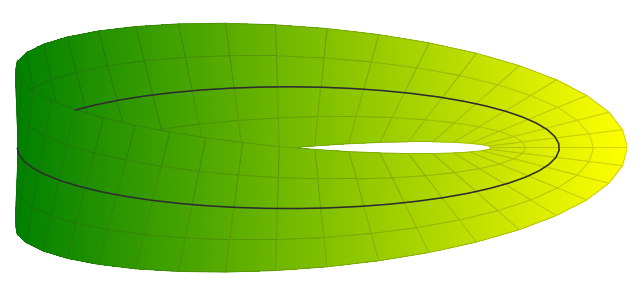
\includegraphics[width=\linewidth]{images/mobius_angle1.png}
    % \begin{tikzpicture}
    % \begin{axis}[
    %     hide axis,
    %     view={0}{40}
    % ]
    % \addplot3 [
    %     surf, shader=faceted interp,
    %     point meta=x,
    %     colormap/greenyellow,
    %     samples=40,
    %     samples y=5,
    %     z buffer=sort,
    %     domain=0:360,
    %     y domain=-0.5:0.5
    % ] (
    %     {(1+0.5*y*cos(x/2)))*cos(x)},
    %     {(1+0.5*y*cos(x/2)))*sin(x)},
    %     {0.5*y*sin(x/2)});
    
    % \addplot3 [
    %     samples=50,
    %     domain=-180:142, % The domain needs to be adjusted manually, depending on the camera angle, unfortunately
    %     samples y=0,
    %     thick
    % ] (
    %     {cos(x)},
    %     {sin(x)},
    %     {0});
    % \end{axis}
    % \end{tikzpicture}
    \caption{M\"{o}bius strip coming from $\phi$.}
    \label{fig:mobius_strip_coming_from_phi_}
  \end{figure}

  It is easy to see that we can adjust the values of the second space in the
  domain for other parameterizations of the M\"{o}bius strip. In particular, we
  can have $\tilde{\phi}$ defined as
  \begin{gather*}
    \tilde{\phi} : (-L, L) \times (-\pi, \pi) \to \mathbb{R}^3 \\
    \tilde{\phi}(\tilde{t}, \tilde{v}) = \left(
      \left( R - \tilde{t} \sin \frac{\tilde{v}}{2} \right) \cos \tilde{v},
      \left( R - \tilde{t} \sin \frac{\tilde{v}}{2} \right) \sin \tilde{v},
      \tilde{t} \cos \frac{\tilde{v}}{2} \right).
  \end{gather*}
  The resulting surface of $\tilde{\phi}$ is shown in
  \cref{fig:mobius_strip_coming_from_tildephi_}.
  \begin{figure}[ht]
    \centering
    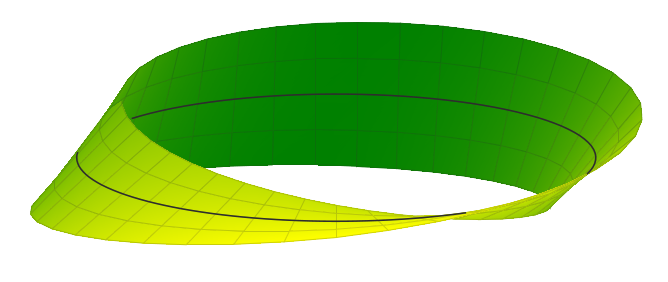
\includegraphics[width=\linewidth]{images/mobius_angle2.png}
    % \begin{tikzpicture}
    % \begin{axis}[
    %     hide axis,
    %     view={90}{40}
    % ]
    % \addplot3 [
    %     surf, shader=faceted interp,
    %     point meta=x,
    %     colormap/greenyellow,
    %     samples=40,
    %     samples y=5,
    %     z buffer=sort,
    %     domain=0:360,
    %     y domain=-0.5:0.5
    % ] (
    %     {(1+0.5*y*cos(x/2)))*cos(x)},
    %     {(1+0.5*y*cos(x/2)))*sin(x)},
    %     {0.5*y*sin(x/2)});
    
    % \addplot3 [
    %     samples=50,
    %     domain=75:232, % The domain needs to be adjusted manually, depending on the camera angle, unfortunately
    %     samples y=0,
    %     thick
    % ] (
    %     {cos(x)},
    %     {sin(x)},
    %     {0});
    % \addplot3 [
    %     samples=50,
    %     domain=265:390, % The domain needs to be adjusted manually, depending on the camera angle, unfortunately
    %     samples y=0,
    %     thick
    % ] (
    %     {cos(x)},
    %     {sin(x)},
    %     {0});
    % \end{axis}
    % \end{tikzpicture}
    \caption{M\"{o}bius strip coming from $\tilde{\phi}$.}
    \label{fig:mobius_strip_coming_from_tildephi_}
  \end{figure}

  \noindent
  \hlbnoted{Claim: the M\"{o}bius strip is not orientable} Notice that the
  domains of $\phi$ and $\tilde{\phi}$, which are
  \begin{equation*}
    U = (-L, L) \times (0, 2 \pi) \text{ and } \tilde{U} = (-L, L) \times (-\pi, \pi),
  \end{equation*}
  are both connected. Since $\phi$ and $\tilde{\phi}$ are both homeomorphisms,
  in particular continuous, both $\phi(U)$ and $\tilde{\phi}(\tilde{U})$ are
  both connected. The intersection of these two parameterizations, which we give
  as $W_1 \cup W_2$, are
  \begin{gather*}
    W_1 = \phi((-L, L) \times (0, \pi)) = \tilde{\phi}((-L, L) \times (0, \pi)) \\
    W_2 = \phi((-L, L) \times (\pi, 2\pi)) = \tilde{\phi} ((-L, L) \times (-\pi, 0))
  \end{gather*}
  Note that $W_1$ and $W_2$ are connected and disjoint. Consider
  \begin{equation*}
    H = \tilde{\phi}^{-1} \circ \phi,
  \end{equation*}
  that takes $(t, v)$ to $(\tilde{t}, \tilde{v})$.

  Now in $W_1$, we have that $\tilde{v} = v$ and $\tilde{t} = t$. It follows
  that
  \begin{equation*}
    (\D H) = \begin{pmatrix} 1 & 0 \\ 0 & 1 \end{pmatrix}
  \end{equation*}
  and so $\det (\D H) = 1$ on $W_1$.

  However, on $W_2$, we have that $\tilde{v} = v - 2 \pi$. Then
  $\frac{\tilde{v}}{2 = \frac{v}{2}} - \pi$. So we have
  \begin{equation*}
    \sin \frac{\tilde{v}}{2} = \sin \frac{v}{2} \text{ and }
    \cos \frac{\tilde{v}}{2} = - \cos \frac{v}{2}.
  \end{equation*}
  We must therefore have that $\tilde{t} = -t$. This is expected from our
  counterclockwise rotation around the anchored point as we revolve around the
  $z$-axis, and eventually turning the line segment upside down. We thus have
  \begin{equation*}
    (\D H) = \begin{pmatrix} 1 & 0 \\ 0 & -1 \end{pmatrix},
  \end{equation*}
  and so $\det (\D H) = -1$ on $W_2$.

  It follows from \cref{propo:non_orientability_checker} that the M\"{o}bius
  strip is non-orientable.
\end{eg}

% section orientability_and_orientation_of_submanifolds_continued (end)

% chapter lecture_25_mar_15th (end)

\tuftepart{Stokes' Theorem and deRham Cohomology}\label{part:stokes_theorem_and_derham_cohomology}

\chapter{Lecture 26 Mar 18th}%
\label{chp:lecture_26_mar_18th}
% chapter lecture_26_mar_18th

\section{Partitions of Unity}%
\label{sec:partitions_of_unity}
% section partitions_of_unity

A \hlnotea{partition of unity} is a tool that allows us to decompose geometric
objects into smaller pieces, each of which can be treated with methods of
standard multivariable calculus.

\begin{note}\label{note:why_partitions_of_unity}
My understanding is that it is a tool to assign a fair weight to each of these
smaller pieces. Thinking ahead, we want to be able to define integration over
manifolds, and we know that a manifold can have infinitely many
parameterizations that cover it. If we simply take a sum of all the integration
over each of the parameterizations, we will end up ``double counting'' the
contribution of \textbf{many} of the points to the integral, which would render
the tool inaccurate.

To amend this problem, first, we want to be able to cover over each point of
$M$ using parameterizations as ``tiny'' as possibly can. This still makes it
difficult for us: there may just be too many parameterizations for us to
calculate, and even more so when $M$ is a `big' manifold. Thus, we will require
that $M$ is \hlnotea{compact}. This will now give us a finite number of
parameterzations to work with.

This makes taking care of double counting in the smaller areas become easier to
deal with. In particular, we will define \hlnotea{smooth bump functions} which
will be our way of giving a weight to each point on the small area, and the
closer we get to the centre, the greater a value we assign. Since each of the
parameterzations are tiny, this gives us a rather fair assignment of weights.

We can do better with this refinement. We can also assign a weight to each of
these parameterzations depending on its contribution, which effectively gives us
a way to average out parameterzations across the board.

The above ideas will be reflected mathematically in the rest of this lecture,
and especially so when we finally define a partition of unity.
\end{note}

\newthought{To define} a partition of unity, we need to first construct
\hlnotea{smooth bump functions}.

\marginnote{
\begin{mnote}
  There is no deep meaning behind the choice of $1$ and $2$ as thresholds. They
  are simply numbers representing some threshold, and we may as well relabel
  them as $\epsilon$ and $\delta$ respectively. Choosing $1$ and $2$ is just for
  conveience.
\end{mnote}
}
\begin{lemma}[Smooth Bump Functions]\index{Smooth Bump Functions}\label{lemma:smooth_bump_functions}
  There exists a smooth function $\chi : \mathbb{R}^k \to \mathbb{R}$ such that
  \sidenote{We can adjust the thresholds $1$ and $2$ so that we still have
  $\chi$ as in the lemma.}
  \begin{marginfigure}
    \centering
    \begin{tikzpicture}
      \draw[->] (-2, 0) -- (2, 0);
      \draw[->] (0, -2) -- (0, 2);
      \draw[fill=blue,fill opacity=0.8] (0, 0) circle(1);
      \draw[fill=red,fill opacity=0.8] (0, 0) circle(0.5);
      \node[label={315:{$1$}}] at (0.4, 0) {};
      \node[label={315:{$2$}}] at (0.9, 0) {};
    \end{tikzpicture}
    \caption{Heat map of the smooth bump function $\chi : \mathbb{R}^2 \to \mathbb{R}$}\label{fig:heat_map_of_chi_}
  \end{marginfigure}
  \begin{table}[ht]
    \centering
    \begin{tabular}{l l l}
      \chi(u) = 1 & & \norm{u} \leq 1 \\
      \chi(u) \in (0, 1) & & 1 < \norm{u} < 2 \\
      \chi(u) = 0 & & \norm{u} \geq 2.
    \end{tabular}
  \end{table}
\end{lemma}

\begin{proof}
  On A4Q7, we showed that there exists a smooth function $f : \mathbb{R} \to
  \mathbb{R}$ such that $f(t) = 0$ for all $t \leq 0$ and $f(t) > 0$ for all $t
  > 0$. Using such an $f$, we define $h : \mathbb{R} \to \mathbb{R}$ such that 
  \begin{equation*}
    h(t) \frac{f(2 - t)}{f(2 - t) + f(t - 1)}.
  \end{equation*}
  Notice that
  \begin{gather*}
    t \leq 1 \implies 2 - t \geq 1 \implies f(2 - t) > 0 \text{ and } f(t - 1) = 0 \\
    t > 1 \implies t - 1 > 0 \implies f(t - 1) > 0 \text{ and } f(2 - t) \geq 0.
  \end{gather*}
  We see the the denominator of $h$ is strictly positive for all $t \in
  \mathbb{R}$. So $h: \mathbb{R} \to \mathbb{R}$ is well-defined. Also, $h$ is
  smooth, since it is composed of smooth functions.

  Now, when $t \geq 2$, we have $2 - t \leq 0$, and so $f(2 - t) = 0$. We have
  that
  \begin{equation*}
    h(t) = 0 \text{ when } t \geq 2.
  \end{equation*}
  When $1 < t < 2$, by our above observation, we have
  \begin{equation*}
    h(t) \in (0, 1) \text{ for } 1 < t < 2.
  \end{equation*}
  When $t \leq 1$, we have $t - 1 \leq 0$, and $f(t - 1) = 0$. Thus
  \begin{equation*}
    h(t) = 1 \text{ for } t \leq 1.
  \end{equation*}
  Our desired result follows by taking $\chi(u) = h(\norm{u})$.
\end{proof}

We also need a special class of local parameterizations, given in the following
lemma.

\marginnote{
\begin{mnote}
  Again, there is no deep meaning behind choosing $3$ as the radius of the ball.
  It simply is out of convenience, and we may as well relabel it as, say,
  $\gamma$.
\end{mnote}
}
\begin{lemma}[Special Parameterizations to Construct Partitions of Unity]\label{lemma:special_parameterizations_to_construct_partitions_of_unity}
  Let $M$ be a $k$-dimensional submanifold of $\mathbb{R}^n$ and let $\phi : U
  \to \mathbb{R}^n$ be any local parameterization of $M$, with image $V \cap M$.
  Let $p \in V \cap M$. Then we can find a local parameterization $\psi : B_3(0)
  \to \mathbb{R}^n$ of $M$, where
  \begin{equation*}
    B_3(0) = \left\{ u \in \mathbb{R}^k \mmid \norm{u} < 3 \right\},
  \end{equation*}
  such that $\psi(0) = p$ and $\psi(B_3(0)) \subseteq \phi(U) = V \cap M$.
\end{lemma}

\marginnote{
\begin{strategy}
The idea of the proof is simple: we know that $p$ has a pre-image, but that may
not be $0$ and $U$ may not be big enough to contain $B_3(0)$. So we just need to
translate $U$ and then scale it accordingly.
\end{strategy}}
\begin{proof}
  Let $u_0 \in U$ be the unique preimage of $p \in V \cap M$, i.e. $\phi(u_0) =
  p$. Since $U$ is open, $\exists \delta > 0$ such that $B_{\delta}(u_0) \subseteq
  U$.

  Let $L : \mathbb{R}^k \to \mathbb{R}^k$ be a translation map that `makes'
  $u_0$ the new origin, i.e. $L(u) = u - u_0$. Let $U'$ be $L(U)$. We have that
  \begin{itemize}
    \item $L$ is a homeomorphism between $U$ and $U'$; and
    \item it is clear that $L(B_{\delta}(u_0)) = B_{\delta}(0)$.
  \end{itemize}
  In particular, $\phi \circ L^{-1}$ is another parameterization of $M$.

  Now let $F : \mathbb{R}^k \to \mathbb{R}^k$ be the map $F(u) =
  \frac{3}{\delta} (u)$, and write $F(U') = U''$. Then
   \begin{itemize}
    \item $F$ is a homeomorphism between $U'$ and $U''$; and
    \item again, $F(B_{\delta}(0)) = B_3(0)$.
  \end{itemize}
  We also have that $\phi \circ L^{-1} \circ F^{-1}$ is another parameterization
  of $M$.

  In particular,  we have that
  \begin{equation*}
    \psi = \phi \circ L^{-1} \circ F^{-1}
  \end{equation*}
  is a homeomorphism, and in particular, $\psi(B_3(0)) \subseteq \phi(U) = V
  \cap M$. Also, we have that $\psi(0) = \phi(u_0) = p$.
\end{proof}

\begin{remark}
  The proof of
  \cref{lemma:special_parameterizations_to_construct_partitions_of_unity} shows
  that we can always find a local parameterization $\phi$ of $M$ such that
  $\phi(0) = p$, and we can find an open ball of any radius around the origin
  such that we contain $p$ in a small open set. In effect, we are can construct
  an open ball around $p$ of any radius induced by a parameterization.
\end{remark}

We also require the following definition in order to define a partition of
unity.

\begin{defn}[Support of a Function]\index{Support}\label{defn:support_of_a_function}
  Let $f : V \to \mathbb{R}$. The \hlnoteb{support} of $f$ is defined as
  \begin{equation*}
    \supp f \coloneqq \overline{\left\{ x \in \mathbb{R}^n : f(x) \neq 0
    \right\}},
  \end{equation*}
  where the bar denotes \hlnotea{closure}.
\end{defn}

\begin{note}
  By the above definition, we know that $\mathbb{R}^n \setminus \supp f$ is an
  \hlimpo{open subset of $\mathbb{R}^n$ where $f$ is identically zero}.
\end{note}

We are now ready to plough through constructing a partition of unity.

\begin{thm}[Partition of Unity]\index{Partition of Unity}\label{thm:partition_of_unity}
  Let $M$ be a compact $k$-dimensional submanifold of $\mathbb{R}^n$, and let
  $\{ V_\alpha \cap M : \alpha \in A \}$ be a cover  of $M$ by the images of
  local parameterizations $\phi_{\alpha}: U_{\alpha} \to \mathbb{R}^n$. Then
  there exists a finite collection of smooth functions $\rho_j : M \to
  \mathbb{R}$ for $j = 1, \ldots, m$ such that
  \begin{enumerate}
  \item for each $j$, the smooth function $\rho_j$ satisfies $0 \leq \rho_j(p)
      \leq 1$ for all $p \in M$;
    \item for each $j$, $\supp \rho_j \subseteq V_{\alpha(j)} \cap M$ for some
      $\alpha(j) \in A$; and
    \item $\sum_{j=1}^{m} \rho_j(p) = 1$ for all $p \in M$.
  \end{enumerate}
  Such a collection of smooth functions is called a \hlnoteb{partition of unity}
  \hldefn{subordinate} \hlnoteb{to this cover}.
\end{thm}

\marginnote{It might be helpful to read \cref{note:why_partitions_of_unity}
before ploughing ahead.}
\begin{proof}
  By \cref{lemma:special_parameterizations_to_construct_partitions_of_unity},
  for each $p \in M$, we can find $\psi_p : B_3(0) \to W_p \cap M$ such
  that
  \begin{itemize}
    \item $\psi_p(0) = p$;
    \item $\psi_p(B_1(0)) = W_p \subseteq V_{\alpha} \cap M$ for some $\alpha
      \in A$. \sidenote{Notice that we defined $W_p$ as the image of
      $\psi_p(B_1(0))$ instead of $\psi_p(B_3(0))$. This is a \hlimpo{sneaky}
      step that we can do to allow ourselves to choose the smallest open ball so
      that it will be useful for us later.}
  \end{itemize}
  Then $\{ W_p : p \in M \}$ forms an open cover of $M$. Since $M$ is
  \hlnotea{compact}, there exists $\{ W_{p, i} \}_{i=1}^{n} \subseteq \{ W_p : p
  \in M \}$ that covers $M$. \sidenote{With this, we have completed the setup,
  putting a finite cover of small open balls on $M$.}
  \begin{figure*}[ht]
    \centering
    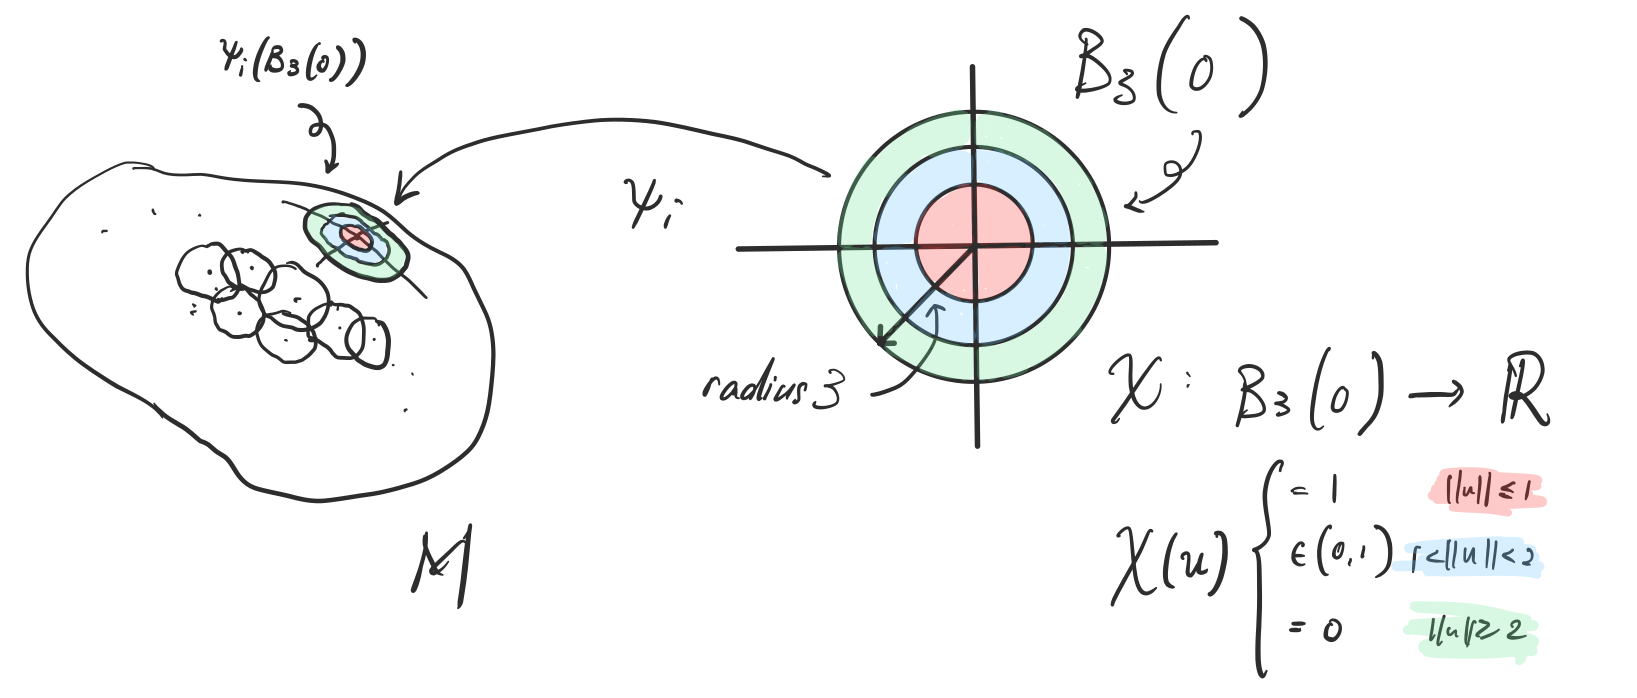
\includegraphics[width=\linewidth]{images/constructing-partition-of-unity.png}
    \caption{Constructing a partition of unity}
    \label{fig:constructing_a_partition_of_unity}
  \end{figure*}

  Define $\zeta_i : M \to \mathbb{R}$ given by
  \begin{equation*}
    \zeta_i = \begin{cases}
      \chi(\psi_i^{-1}(q)) & q \in \psi_i(B_3(0)) \\
      0          & q \in M \setminus \psi_i(\overline{B_2(0)})
    \end{cases},
  \end{equation*}
  where $\chi$ is a \hyperref[lemma:smooth_bump_functions]{smooth bump
  function}. \sidenote{With this, we have assigned a weightage to each point on
  the manifold given a parameterization.}
  
  Notice that each of the $\zeta_i$'s is smooth since $\chi \circ \psi^{-1}$ is
  smooth for each $p \in \psi_i(B_3(0))$. Since $\supp \chi \subseteq
  \overline{B_2(0)}$, $\zeta_i$ is identically zero on $M \setminus
  \psi(\overline{B_2(0)})$. This implies that $\zeta_i$ is indeed smooth on $M$.
  \sidenote{It is important to us that all the $\zeta_i$'s are continuous, since
  we want to assign a weight to each parameterization in a smooth' manner. Its
  importance will surface later on.}

  Now define $\rho_i : M \to \mathbb{R}$ such that
  \begin{equation*}
    \rho_i(p) = \frac{\zeta_i(p)}{\sum_{j=1}^{n} \zeta_j(p)},
  \end{equation*}
  for any $p \in M$. Note that that the \hlnotea{denominator} of each $\rho_i$
  is greater than $0$, since $p \in W_{q, j} = \psi_j(B_1(0))$ for some $j$, since the $W_{q,
  j}$'s form a cover of $M$. \sidenote{This is where we use the \hlimpo{sneaky}
  step. Notice that should we not have picked the $W_p$'s in such a way the
  definition of the $\rho_i$'s would be in deep trouble.}

  We shall now verify the conditions:
  \begin{enumerate}
    \item It is clear that $0 \leq \rho_i(p) \leq 1$, since we clearly have
      \begin{equation*}
        0 \leq \zeta_i(p) \leq \sum_{j=1}^{n} \zeta_i(p);
      \end{equation*}
    \item Notice that
      \begin{equation*}
        \rho_i(p) = 0 \iff \zeta_i(p) = 0 \iff p \in M \setminus
        \overline{B_2(0)} \iff p \notin W_{q, i}
      \end{equation*}
      Thus $\supp \rho_i \subseteq W_{q, i} \cap M \subseteq V_{\alpha(i)} \cap
      M$ for some $\alpha(i) \in A$; and
    \item it is clear that
      \begin{equation*}
        \sum_{i=1}^{n} \rho_i(p) = \sum_{i=1}^{n}
        \frac{\zeta_i(p)}{\sum_{j=1}^{n} \zeta_j(p)} = 1.
      \end{equation*}
  \end{enumerate}
  Finally, we note that since $\rho_i$ is a composition of smooth functions,
  $\rho_i$ itself is also smooth, which is what we need.
\end{proof}

\begin{remark}
  By \citet{karigiannis2019}, the compactness assumption is actually not
  necessary; we can construct partitions of unity even on noncompact
  submanifolds on $\mathbb{R}^n$, but the process is considerably more
  difficult.
\end{remark}

% section partitions_of_unity (end)

% chapter lecture_26_mar_18th (end)

\chapter{Lecture 27 Mar 20th [dirty]}%
\label{chp:lecture_27_mar_20th}
% chapter lecture_27_mar_20th

\section{Partitions of Unity (Continued)}%
\label{sec:partitions_of_unity_continued}
% section partitions_of_unity_continued

\begin{propo}
  Let $M$ be a $k$-dimemensional submanifold of $\mathbb{R}^n$ and suppose that
  there exists a cover of $M$ by local parameterizations such that all the
  transition maps $\phi_{\beta \alpha}$ satisfy $\det (\D \phi_{ \beta \alpha }) >
  0$. Then $M$ is oriented. That is, there exists a nowhere vanishing $k$-form
  $\mu$ on $M$, such that all these local parameterizations are compatible with
  $\mu$.
\end{propo}

\begin{note}
  The above result is true in general when used with a general partition of
  unity.
\end{note}

\begin{proof}
  
\end{proof}

% section partitions_of_unity_continued (end)

% chapter lecture_27_mar_20th (end)

\chapter{Lecture 28 Mar 22nd [dirty]}%
\label{chp:lecture_28_mar_22nd}
% chapter lecture_28_mar_22nd

\section{Integration of Forms (Continued)}%
\label{sec:integration_of_forms_continued}
% section integration_of_forms_continued

From last time, let $M = \phi(U) = \tilde{\phi}(\tilde{U})$ be a parameterized
$k$-dimensional submanfold.

Let $w \in \Omega^k(M)$. We defined
\begin{equation*}
  \int_{M} w = \int_{U} \phi^* w = \int_{\tilde{U}} \tilde{\phi}^* w .
\end{equation*}
We showed that this is well-defined iff $\phi, \tilde{\phi}$ determine the same
orientation iff $\det (\D (\tilde{\phi}^{-1} \circ \phi)) > 0$.

\newthought{Now let} $M$ be a compact $k$-dimensional submanifold of
$\mathbb{R}^n$. Let $w \in \Omega^k(M)$, where $\supp(w)$ is a closed subset of
$M$, which is compact, and so $\supp(w)$ is compact. We want to define
\begin{equation*}
  \mathbb{R} \ni \int_{M} w. 
\end{equation*}

The idea is to use \hyperref[sec:partitions_of_unity_continued]{partitions of
unity} to decompose $\omega$ into a finite sum of smooth $k$-forms, with each of them
\hlnotea{compactly supported} in the image of the single parameterization.

We handle these as we did last time and add some results. We need to show that
this process is independent of our choices \sidenote{\hlwarn{elaborate}}.

Let $\{ V_\alpha \cap M : \alpha \in A \}$ be a cover of $M$ given by images of
local parameterizations $\phi_\alpha : U_\alpha \to \mathbb{R}^n$ of $M$, all of
which are \hlnotea{compatible} with the given orientation on $M$.

Let $\{ \rho_j : j = 1, \ldots, m \}$ be a partition of unity corresponding to
the above cover, where $\rho_j : M \to \mathbb{R}$ is smooth,
\begin{itemize}
  \item $0 \leq \rho_j(p) \leq 1$ for each $p$, and
  \item $\sum_{j=1}^{m} \rho_j = 1$,
\end{itemize}
where $\supp(\rho_j) \subseteq V_{\alpha(j)} \cap M$ for some $\alpha(j) \in A$.
Let us denote $V_{\alpha(j)} = V_j$, and $\phi_{\alpha(j)} = \phi_j$. Note that
\begin{equation*}
  \bigcup_{j=1}^{m} V_j \supseteq M.
\end{equation*}

Observe that
\begin{equation*}
  \omega = 1 \cdot \omega = \left( \sum_{j=1}^{m} \rho_j \right) \omega =
  \sum_{j=1}^{m} (\rho_j \omega),
\end{equation*}
and
\begin{equation*}
  \supp(\rho_j \omega) \subseteq \supp(\rho_j) \subseteq V_j \cap M.
\end{equation*}
Hence, we can consider $\rho_j \omega$ as a smooth $k$-form on $V_j$ and define
\begin{equation*}
  \int_{M} \rho_j \omega := \int_{V_j \cap M} \rho_j \omega = \int_{U_j}
  \phi_j^* (\rho_j \omega).
\end{equation*}
This is sensible because $\rho_j \omega$ vanishes outside of $V_j \cap M$.

Thus we define
\begin{equation*}
  \int_{M} \omega = \int_{M} \left( \sum_{j=1}^{m} \rho_j \omega \right) :=
  \sum_{j=1}^{m} \int_{M} \rho_j \omega \in \mathbb{R}. 
\end{equation*}

Now we need to show that the result is independent of the choice of the
parameterization.

Let $\{ W_\beta \cap M : \beta \in B \}$ be a cover of $M$ by images of local
parameterizations $\psi_\beta$ of $M$ compatible with the given orientation.

Let $\{ \sigma_i : i = 1, \ldots, l \}$ be a partition of unity for this cover,
with the usual properties \sidenote{\hlwarn{needs expansion, but we know what
this is.}}.

\marginnote{Note that
\begin{equation*}
  \supp(\rho_j \omega) \subseteq V_j \cap M,
\end{equation*}
and
\begin{equation*}
  \supp(\sigma_i \rho_j \omega) \subseteq W_i \cap V_j \cap M.
\end{equation*}
}
By our first choice, we have
\begin{align*}
  \int_{M} \omega &= \sum_{j=1}^{m} \int_{M} \rho_j \omega = \sum_{j=1}^{m}
  \int_{M} \left( \sum_{i=1}^{l} \sigma_i \right) \rho_j \omega \\
  & = \sum_{j=1}^{m} \sum_{i=1}^{l} \int_{M} \sigma_i \rho_j \omega  =
  \sum_{i=1}^{l} \sum_{j=1}^{m} \int_{M} \rho_j \sigma_i \omega \\
  &= \sum_{i=1}^{l} \int_{M} \left( \sum_{j=1}^{m} \rho_j \right) \sigma_i \omega = \sum_{i=1}^{l} \int_{M} \sigma_i \omega = \int_{M} \omega,
\end{align*}
where the final equality is by our second choice.

\begin{thm}[Stokes' Theorem (First Version)]\index{Stokes' Theorem}\label{thm:stokes_theorem_first}
  Suppose $M$ is a compact and oriented $k$-dimensional submanifold of
  $\mathbb{R}^n$, and $\omega \in \Omega^{k - 1}(M)$ and $\dif{\omega} \in
  \Omega^k(M)$, then
  \begin{equation*}
    \int_{M} \dif{\omega} = 0. 
  \end{equation*}
\end{thm}

We will prove a result more general than the above.

More generally, if $M$ is a $k$-dimensional, compact, and oriented submanifold,
\hlnotea{with boundary} (defined later), then $\partial M$ (the boundary) is a
compact, oriented $(k - 1)$-dimensional submanifold, such that
\begin{equation*}
  \int_{M} \partial M = \int_{\partial M} \omega. 
\end{equation*}

% section integration_of_forms_continued (end)

\section{Submanifolds with Boundary}%
\label{sec:submanifolds_with_boundary}
% section submanifolds_with_boundary

\begin{defn}[Half Space]\index{Half Space}\label{defn:half_space}
  We define the \hlnoteb{half space} of $\mathbb{R}^n$ as
  \begin{equation*}
    \mathbb{H}^n := \left\{ x \in \mathbb{R}^n : x^1 \leq 0 \right\}.
  \end{equation*}
\end{defn}

\begin{note}
  The half space is closed but unbounded.
\end{note}

\begin{defn}[Boundary of the Half Space]\index{Boundary of the Half Space}\label{defn:boundary_of_the_half_space}
  We define the \hlnoteb{boundary of the half space as}
  \begin{equation*}
    \partial \mathbb{H}^n := \left\{ x \in \mathbb{R}^n : x^1 = 0 \right\}
    \simeq \mathbb{R}^{n - 1}.
  \end{equation*}
\end{defn}

\begin{defn}[Open Subset in a Half Space]\index{{Open set in a Half Space}}\label{defn:open_subset_in_a_half_space}
  A subset $A$ of $\mathbb{H}^n$ is said to be \hlnoteb{open} in $\mathbb{H}^n$ if $A = U
  \cap \mathbb{H}^n$ where $U \subseteq \mathbb{R}^n$ is open.
\end{defn}

\begin{note}
  A subset $A$ which is open in $\mathbb{H}^n$ may or may not be open in
  $\mathbb{R}^n$.
\end{note}

\begin{lemma}[Characterization of Open Sets in a Half Space]\label{lemma:characterization_of_open_sets_in_a_half_space}
  Let $A, B \subseteq \mathbb{H}^n$. If $A \subseteq \mathbb{R}^n$, then $A$ is
  open in $\mathbb{H}^n$. Suppose $B \cap \partial \mathbb{H}^n = \emptyset$. If
  $B$ is open in $\mathbb{H}^n$, then $B$ is open in $\mathbb{R}^n$.
\end{lemma}

\begin{proof}
  We have that $A$ is open in $\mathbb{R}^n$ and contained in $\mathbb{H}^n$.
  Then we simply need to take $U = A \subseteq \mathbb{R}^n$. Thus $A$ is open
  in $\mathbb{H}^n$.

  Suppose $B \cap \partial \mathbb{H}^n = \emptyset$. Let $B$ be open in
  $\mathbb{H}^n$. Then $\exists U \subseteq \mathbb{R}^n$ open such that $B = U
  \cap \mathbb{H}^n$. Let $W = \mathbb{H}^n \setminus \partial \mathbb{H}^n =
  \left\{ x \in \mathbb{R}^n : x^1 < 0 \right\}$,
  which is open in $\mathbb{R}^n$. It follows that $B \subseteq W$ and so $B = U
  \cap W$, which is an intersection of open sets in $\mathbb{R}^n$. Thus $B$ is
  open in $\mathbb{R}^n$.
\end{proof}

\begin{defn}[Interior point in the Half Space]\index{Interior point in the Half Space}\label{defn:interior_point_in_the_half_space}
  Let $A \subseteq \mathbb{H}^n$ be open in $\mathbb{H}^n$. Then $p \in A$ is
  called a \hlnoteb{interior point} of $A$ if $p \notin \partial \mathbb{H}^n$
  \sidenote{We have that $\exists \epsilon > 0$ such that $B(p, \epsilon)
  \subseteq A$.}.
\end{defn}

\begin{defn}[Boundary point in the Half Space]\index{Boundary point in the Half Space}\label{defn:boundary_point_in_the_half_space}
  Let $A \subseteq \mathbb{H}^n$ be open in $\mathbb{H}^n$. Then $p \in A$ is
  called an \hlnoteb{boundary point} of $A$ if $p \in \partial \mathbb{H}^n$
  \sidenote{In this case, we have that $\forall \epsilon > 0$ such that $B(p,
  \epsilon) \subsetneq A$.}.
\end{defn}

\begin{defn}[Smooth functions in the Half Space]\index{Smooth functions in the Half Space}\label{defn:smooth_functions_in_the_half_space}
  Let $A \subseteq \mathbb{H}^n$ be open in $\mathbb{H}^n$, $f : A \to
  \mathbb{H}^n$ and $p \in A$. We say that $f$ is \hlnoteb{smooth} at $p$ if
  $\exists$ an open neighbourhood $U \subseteq \mathbb{R}^n$ of $p$ and a map
  $\tilde{f} : U \to \mathbb{R}^n$ such that
  \begin{enumerate}
    \item $f \restriction_{U \cap A} = \tilde{f} \restriction_{U \cap A}$ and
    \item $\tilde{f}$ is smooth at $p$.
  \end{enumerate}
\end{defn}

\begin{remark}
  \begin{enumerate}
    \item If $p$ is an interior point of $A$, then this \hlnotea{agrees} with
      the usual definition of smoothness because we can just talk about $U =
      B(p, \epsilon) \subseteq A$, and $\tilde{f} = f \restriction_{U}$. So if
      $f$ is smooth at $p$, we define
      \begin{equation*}
        (\D f)_p := (\D \tilde{f})_p.
      \end{equation*}
  \end{enumerate}
\end{remark}

\hlbnoted{Claim} $(\D f)_p$ is well-defined (i.e. indeppendent of the choice of
$\tilde{f}$).

\begin{defn}[Submanifold with Boundary]\index{Submanifold with Boundary}\label{defn:submanifold_with_boundary}
  Let $M \subseteq \mathbb{R}^n$. We say that $M$ is a \hlnoteb{$k$-dimensional
  submanifold with boundary} of $\mathbb{R}^n$ if there exists a cover of $M$ by
  subsets $\{ V_\alpha : \alpha \in A \}$ and a collection of subsets $\{
  U_\alpha : \alpha \in A \} \subseteq \mathcal{P}(\mathbb{H}^k)$, each
  $U_\alpha$ open in $\mathbb{H}^k$, and maps $\phi_\alpha : U_\alpha \to
  \mathbb{R}^n$, such that each
  \begin{enumerate}
    \item $\phi_\alpha$ is a homeomorphism of $U_\alpha$ onto
      $\phi_\alpha(U_\alpha) = V_\alpha \cap M$, and
    \item $\phi_\alpha$ is a smooth immersion.
  \end{enumerate}
\end{defn}

% section submanifolds_with_boundary (end)

% chapter lecture_28_mar_22nd (end)

\chapter{Lecture 29 Mar 25th [dirty]}%
\label{chp:lecture_29_mar_25th}
% chapter lecture_29_mar_25th

\section{Submanifold with Boundary (Continued)}%
\label{sec:submanifold_with_boundary_continued}
% section submanifold_with_boundary_continued

We defined, in the last lecture, what a submanifold with boundary is. We saw
that a $k$-dimensional submanifold with boundary is a collection of overlapping
pieces, each homeomorphic to an open set in $\mathbb{H}^k$.

Suppose $\phi_\alpha(A_\alpha) \cap \phi_b(A_\beta) \neq \emptyset$. We define
the transition map
\begin{equation*}
  \phi_{\beta\alpha} : \phi_\alpha^{-1}(\phi_\alpha(A_\alpha) \cap
  \phi_\beta(A_\beta)) \to \phi_\beta^{-1}(\phi_\alpha(A_\alpha) \cap
  \phi_\beta(A_\beta))
\end{equation*}
by
\begin{equation*}
  \phi_{\beta\alpha} = \phi_\beta^{-1} \circ \phi_\alpha.
\end{equation*}
This is the same definition as \cref{defn:transition_map}, but this time, our
open sets come from $\mathbb{H}^k$.

We still have \cref{propo:transition_maps_are_diffeomorphisms}, i.e. 
transition maps are diffeomorphisms, and the same proof can be applied.

\begin{remark}
  Using the local parameterizations $\phi_\alpha$ for a submanifold with boundary
  $M$, and the fact that transition maps are diffeomorphisms, we can now define
  \begin{itemize}
    \item smooth functions on $M$,
    \item smooth curves on $M$, 
    \item smooth vector fields on $M$,
    \item smooth differential forms ($r$-forms) on $M$ for $0 \leq r \leq k$,
    \item orientations and orientability,
    \item partitions of unity, and
    \item integration of smooth $k$-forms if $M$ is oriented and compact,
  \end{itemize}
  all exactly as before. The only difference is that we replace open set in
  $\mathbb{R}^k$ by open sets in $\mathbb{H}^k$.
\end{remark}

\begin{remark}
  If all the $A_\alpha$'s are actually open in $\mathbb{R}^k$, then $M$ is a
  $k$-dimensional submanifold in the previous sense.
\end{remark}

\newthought{So we defined} what a submanifold with boundary is, but what is a
boundary?

\begin{defn}[Boundary Point on a Submanifold]\index{Boundary Point on a Submanifold}\label{defn:boundary_point_on_a_submanifold}
  Let $M$ be a $k$-dimensional submanifol with boundary. A point $p \in M$ is
  called a \hlnoteb{boundary point} of $M$ if there exists a local
  parameterization $\phi_\alpha : A_\alpha \to M$ with $p \in
  \phi_\alpha(A_\alpha)$ such that $\phi_\alpha^{-1} (p) \in \partial
  \mathbb{H}^k$.
\end{defn}

Of course, we can ask ourselves if the above definition is well-defined. That
is, can there but a $\phi_\beta$ such that $\phi_\beta^{-1}(p)$ is not on
$\partial A_\beta$?

\begin{propo}[Well-definedness of the Boundary of a Manifold]\label{propo:well_definedness_of_the_boundary_of_a_manifold}
  Let $p \in M$ be a boundary point. Then $\phi_\beta^{-1}(p) \in \partial
  \mathbb{H}^k$ for all local parameterizations $\phi_\beta : A_\beta \to
  \mathbb{R}^n$ of  $M$.
\end{propo}

\begin{proof}
  Suppose not. Let $u_\alpha = \phi_\alpha^{-1}(p) \in \partial \mathbb{H}^k$ so
  that $u_\alpha$ is a boundary point of $A_\alpha$, and suppose there exists
  $\phi_\beta$ a parameterization such that $u_\beta = \phi_\beta^{-1}(p) \notin
  \partial \mathbb{H}^k$, i.e. $u_\beta$ is an interior point of $A_\beta$.

  Now the transition map
  \begin{equation*}
    \phi_{\alpha\beta} = \phi_\alpha^{-1} \circ \phi_\beta
  \end{equation*}
  is a diffeomorphism between the opens subsets of $\mathbb{H}^k$ that takes
  $u_\beta$ to $\phi_{\alpha\beta}(u_\beta) = u_\alpha$. Since $u_\beta$ is an
  interior point of $A_\beta$, there exists an open set $W \subseteq
  \mathbb{R}^k$ such that $u_\beta \in W$ in the domain of $\phi_{\alpha\beta}$.
  Then $W \cap \partial \mathbb{H}^k = \emptyset$.

  Restrict the diffeomorphism $\phi_{\alpha\beta}$ to $W$, and so $(\D
  \phi_{\alpha\beta})_{u_\beta}$ is invertble. By the inverse function theorem,
  $\exists \tilde{W} \subseteq W$ open in $\mathbb{R}^k$, with $u_\alpha \in
  \tilde{W}$ such that $\phi_{\alpha\beta}$ maps $\tilde{W}$ diffeomorphically
  onto $\phi_{\alpha\beta}(W)$, which is an open set in $\mathbb{R}^k$. Thus
  \begin{equation*}
    u_\alpha = \phi_{\alpha\beta}(u_\beta) \in \phi_{\alpha\beta} (W) \subseteq
    \mathbb{R}^k \text{ open. }
  \end{equation*}
  So $\exists Y \subseteq \mathbb{R}^k$ open, with $u_\beta \in Y \subseteq
  \phi_{\alpha\beta}(\tilde{W}) \subseteq \phi_{\alpha\beta}(W) \subseteq
  A_{\alpha}$. Thus there exists points in $A_\alpha$ with $u^1 > 0$, which is
  impossible since we are in $\mathbb{H}^k$.
\end{proof}

\begin{defn}[Boundary of a Submanifold]\index{Boundary of a Submanifold}\label{defn:boundary_of_a_submanifold}
  Let $M$ be a $k$-dimensional submanifold with boundary. The \hlnoteb{boundary}
  of $M$ is denoted $\partial M$ and is the subset of $M$ consisting of all
  boundary points of $M$.
\end{defn}

\begin{note}
  A submanifold $M$ with boundary is an ordinary submanifold (i.e. submanifold
  without boundary) iff $\partial M = \emptyset$.
\end{note}

\begin{propo}[Dimension of the Boundary of a Submanifold]\label{propo:dimension_of_the_boundary_of_a_submanifold}
  Let $M$ be a $k$-dimensional submanifold with boundary. Suppose $\partial M
  \neq \emptyset$. Then $\partial M$ is a $(k - 1)$-dimensional submanifold with
  boundary, i.e. $\partial(\partial M) = \emptyset$.
\end{propo}

\begin{proof}
  We need to find a cover of $\partial M$ by local parameterizations whose
  domains are open sets in $\mathbb{R}^{k-1}$.

  Let  $p \in \partial M \subseteq M$, so that there exists a local
  parameterization $\phi$ of $M$ such that $\phi : A \to \mathbb{R}^n$, where $A$ 
  is open in $\mathbb{H}^k$, with $p \in \phi(A)$. Let $\hat{\phi}$ be the
  restriction of $\phi$ to $A \cap (\partial \mathbb{H}^k)$.

  Let $\hat{A} = A \cap (\partial \mathbb{H}^k)$. \hlbnotec{Check} $\hat{A}$ is
  open in $\partial \mathbb{H}^k \simeq \mathbb{R}^{k-1}$. Let
  \begin{equation*}
    \hat{\phi}(p) = (0, u^2, \ldots, u^k) \in (\partial \mathbb{H}^k) \cap A,
  \end{equation*}
  and
  \begin{equation*}
    \hat{u} = (u^2, \ldots, u^k) \in \hat{A}.
  \end{equation*}
  Then
  \begin{equation*}
    \hat{\phi}(\hat{u}) = p \in \partial M.
  \end{equation*}
  We need to show that $\hat{\phi} : \hat{A} \to \mathbb{R}^n$, where $\hat{A}$ 
  is open in $\mathbb{R}^{k-1}$, is a smooth immersion and a homeomorphism onto
  its image.

  Since $\phi$ is smooth at $v \in A \cap \partial \mathbb{H}^k$, we have that
  $\hat{\phi}$ is smooth at $\hat{v} \in \hat{A}$. The Jacobian
  \begin{equation*}
    (\D \hat{\phi})_{\hat{u}} = \begin{pmatrix}
      \frac{\partial \phi^1}{\partial u^2} \at{\hat{u}}{} & \hdots &
      \frac{\partial \phi^1}{\partial u^k}
      \at{\hat{u}}{} \\
      \vdots & & \vdots \\
      \frac{\partial \phi^n}{\partial u^2} \at{\hat{u}}{} & \hdots & \frac{\partial \phi^n}{\partial u^k} \at{\hat{u}}{}
    \end{pmatrix}.
  \end{equation*}
  $\phi$ is an immersion, so columns of $(\D \phi)_{\hat{u}}$ are linearly
  independent, so columns are $(\D \hat{\phi})_{\hat{u}}$ are still linearly
  independent, hence $\hat{\phi}$ is an immersion.

  So $\hat{\phi}$ is continuous because it is the restriction of a continuous
  map. Thus
  \begin{equation*}
    (\hat{\phi})^{-1} : \hat{\phi}(\hat{A}) \to \hat{A}
  \end{equation*}
  is the restriction of $\phi^{-1}$ to $\phi(\hat{A})$, and so it is also
  continuous. Thus $\hat{\phi}$ is a homeomorphism onto its image. Thus
  $\hat{\phi}$ is a local parameterization for $\partial M$.
\end{proof}

% section submanifold_with_boundary_continued (end)

% chapter lecture_29_mar_25th (end)

\chapter{Lecture 31 Mar 29th [dirty]}%
\label{chp:lecture_31_mar_29th}
% chapter lecture_31_mar_29th

\section{Stokes' Theorem (Continued)}%
\label{sec:stokes_theorem_continued}
% section stokes_theorem_continued

\begin{proof}[Stokes' Theorem (Continued)]
  We reduced the proof to showing that following: given $A$ open in
  $\mathbb{H}^k$ and $\hat{A} = A \cap (\partial \mathbb{H}^k)$ open in
  $\mathbb{R}^{k-1}$. Let $\phi : A \to \mathbb{R}^n$ and $\hat{\phi} = \phi
  \restriction_{\hat{A}} \hat{A} \to \mathbb{R}^n$ be a parameterizations. Let
  $\eta \in \Omega^{k-1}(\phi(A))$, where $\supp(\eta)$ is compact. We want to
  be able to show that
  \begin{equation*}
    \int_{A_j} \dif{(\phi_j^*(\rho_j \omega))} = \int_{\hat{A}_j}
    \hat{\phi}_j^*(\rho_j \omega) 
  \end{equation*}
  for all $j$.

  First, some observations are needed. Let us write
  \begin{equation}\label{eq:stokes_proof_eq_2}
    \Omega^k(A) \ni \phi^* \eta = \sum_{i=1}^{k} (-1)^{i-1} h_i \dif{u^1} \land
    \hdots \land \hat{\dif{u^i}} \land \hdots \land \dif{u^k},
  \end{equation}
  where the $(-1)^{i-1}$ instead of $(-1)^{k-1}$ for convenience, and $h_i \in
  C^\infty(A)$ has compact support. Now note that  $\hat{\phi} = \phi \circ j$,
  where $j : \mathbb{R}^{k-1} \to \mathbb{R}^k$ is the smooth map
  \begin{equation*}
    j(u^2, \ldots, u^k) = (-0, u^2, \ldots, u^k).
  \end{equation*}
  Thus we have that $\hat{\phi}^* = j^* \phi^*$. In particular, $j^* \dif{u^i} =
  \dif{u^i}$ for $i > 1$, and $j^* \dif{u^1} = 0$. By taking $j^*$ on
  \cref{eq:stokes_proof_eq_2}, we have
  \begin{align*}
    \hat{\phi}^* \eta &= j^* \hat{\phi} \eta \\
                      &= j^* \left( \sum_{i=1}^{k} (-1)^{i-1} h_i \dif{u^1}
                      \land \hdots \hat{\dif{u^i}} \land \hdots \land \dif{u^k}
                    \right) \\
                      &= j^*(h_1 \dif{u^2} \land \hdots \land \dif{u^k}) \\
                      &= \hat{h}_1 \dif{u^2} \land \hdots \land \dif{u^k}
                      \tag{$\dagger$}\label{eq:stokes_proof_eq_3},
  \end{align*}
  where $\hat{h}_1 = j^* h_1$. That is, we have
  \begin{equation*}
    \hat{h}_1(u^2, \ldots, u^k) = h_1(0, u^2, \ldots, u^k).
  \end{equation*}
  Now taking $\dif{}$ of \cref{eq:stokes_proof_eq_2}, we have
  \begin{align*}
    \dif{(\phi^* \eta)}
    &= \sum_{i=1}^{k} (-1)^{i-1} \left( \sum_{l=1}^{k} \frac{\partial
      h_i}{\partial u^l} \dif{u^l} \right) \land \dif{u^1} \land \hdots \land
      \hat{\dif{u^i}} \land \hdots \land \dif{u^k} \\
    &= \sum_{i=1}^{k} (-1)^{i-1} \frac{\partial h_i}{\partial u^i} \dif{u^i}
      \land \dif{u^1} \land \hdots \land \hat{\dif{u^i}} \land \hdots \land
      \dif{u^k} \\
    &= \left( \sum_{i=1}^{k} \frac{\partial h_i}{\partial u^i} \right) \dif{u^1}
      \land \hdots \land \dif{u^k} \tag{*}\label{eq:stokes_proof_eq_4}.
  \end{align*}

  We are now ready to take on what we want to show.

  \noindent
  \hlbnoted{Case 1} Suppose $A$ is open in $\mathbb{R}^k$, with $A \cap \partial
  \mathbb{H}^k = \emptyset$ and $\supp(h_i)$ is compact. So there exists a box
  $K = [a^1, b^1] \times \hdots \times [a^k, b^k]$ be a box in $bb^k$ that
  completes contains $\supp h_i$ in its interior. Now extend each of the $h_i$ 
  by zero to a smooth function on $\mathbb{R}^k$. Using
  \cref{eq:stokes_proof_eq_4}, we have that the LHS of what we want is
  \begin{align*}
    \int_{A} \dif{\phi^* \eta}
    &= \int_{A} \left( \sum_{i=1}^{k} \frac{\partial h_i}{\partial u^i}
    \dif{u^1} \land \hdots \land \dif{u^k} \right) \\
    &= \sum_{i=1}^{k} \int_{A} \frac{\partial h_i}{\partial u^i} \dif{u^1}
    \hdots \dif{u^k} \\
    &= \sum_{i=1}^{k} \int_{a^1}^{b^1} \hdots \int_{a^k}^{b^k} \frac{\partial
    h_i}{\partial u^i} \dif{u^1} \hdots \dif{u^k}.
  \end{align*}
  By \hlnotea{Fubini's Theorem}, we can integrate in any order. For the
  $i$\textsuperscript{th} integral, integrate first wrt $u^i$. Then by the
  \hlnotea{Fundamental Theorem of Calculus}, we have
  \begin{align*}
    &\int_{a^i}^{b^i} \frac{\partial h_i}{\partial u^i} \dif{u^i} \\
    &= h_i(u^1, \ldots, u^{i-1}, b^i, u^{i+1}, \ldots, u^k) - h_i(u^1, \ldots,
    u^{i-1}, a^i, u^{i+1}, \ldots, u^k) \\
    &= 0 - 0 = 0,
  \end{align*}
  since $h_i$ is supported inside the interior of $K$. Thus all the integrals
  above are zero, i.e. the LHS of what we want is zero in this case.

  On the other hand, since $A$ is an open set in $\mathbb{R}^k$, we have that $A
  \cap \partial \mathbb{H}^k = \emptyset$, so $\supp h_1 \subseteq A$ does not
  intersect $\partial \mathbb{H}^k$. Thus $h_1 = j^* h_1 = 0$. By
  \cref{eq:stokes_proof_eq_3} and the fact that $K \cap \partial \mathbb{H}^k =
  [a^2, b^2] \times \hdots \times [a^k, b^k]$, we have
  \begin{align*}
    \int_{A} \hat{\phi}^* \eta
    &= \int_{K \cap \partial \mathbb{H}^k} \hat{\phi}^* \eta = \int_{K \cap
    \partial \mathbb{H}^k} h_1 \dif{u^2} \land \hdots \land \dif{u^k} \\
    &= \int_{a^2}^{b^2} \hdots \int_{a^k}^{b^k} \hat{h}_i \dif{u^2} \hdots
    \dif{u^k} = 0.
  \end{align*}
  This completes Case 1.

  \noindent
  \hlbnoted{Case 2} Suppose $A$ is not open in $\mathbb{R}^k$. Then $A \cap
  \partial \mathbb{H}^k \neq \emptyset$. This time, let
  \begin{equation*}
    K = [a^1, 0] \times [a^2, b^2] \times \hdots \times [a^k, b^k]
  \end{equation*}
  be a box in $\mathbb{H}^k$ such that $\supp h_i$ is contained in the union of
  the interior of $K$ with $\partial \mathbb{H}^k$. Once again, extend each
  $h_i$ by zero to a smooth function on $\mathbb{H}^k$. Using
  \cref{eq:stokes_proof_eq_4}, we have
  \begin{align*}
    \int_{A} \dif{(\phi^* \eta)}
    &= \int_{K} \dif{(\phi^* \eta)} \\
    &= \int_{K} \sum_{i=1}^{k} \left( \frac{\partial h_i}{\partial u^i} \right)
    \dif{u^1} \land \hdots \land \dif{u^k} \\
    &= \int_{a^1}^{0} \int_{a^2}^{b^2} \hdots \int_{a^k}^{b^k} \left(
    \sum_{i=1}^{k} \frac{\partial h_i}{\partial u^i} \right) \dif{u^1} \hdots
    \dif{u^k} \\
    &= \sum_{i=1}^{k} \int_{a^1}^{0} \int_{a^2}^{b^2} \hdots \int_{a^k}^{b^k}
    \frac{\partial h_i}{\partial u^i} \dif{u^1} \hdots \dif{u^k}.
  \end{align*}
  Since the $h_i$'s are smooth, we can apply \hlnotea{Fubini's Theorem} and
  integrate in any order we want. For the $i$\textsuperscript{th} integral,
  integrate first wrt $u^i$. If $i > 1$, then by the \hlnotea{Fundamental
  Theorem of Calculus}, we have
  \begin{align*}
    &\int_{a^1}^{0} \frac{\partial h_1}{\partial u^1} \dif{u^1} \\
    &= h_1(0, u^2, \ldots, u^k) - h_1(a^1, \ldots, u^k) \\
    &= \hat{h}_1(u^2, \ldots, u^k) - 0 \\
    &= \hat{h}_1(u^2, \ldots, u^k).
  \end{align*}
  Thus we have that the LHS of our desired equation is
  \begin{equation*}
    \int_{A} \dif{(\phi^* \eta)} = \int_{a^2}^{b^2} \hdots \int_{a^k}^{b^k}
    \hat{h}_1 \dif{u^2} \hdots \dif{u^k}.
  \end{equation*}
  By \cref{eq:stokes_proof_eq_4} and the fact that $K \cap \dif{\mathbb{H}^k} =
  [a^2, b^2] \times \hdots \times [a^k, b^k]$, we have that
  \begin{align*}
    \int_{\hat{A}} \hat{\phi}^* \eta
    &= \int_{K \cap \partial \mathbb{H}^k} \hat{\phi}^* \eta \\
    &= \int_{K \cap \partial \mathbb{H}^k} h_1 \dif{u^2} \land \hdots \land
    \dif{u^k} \\
    &= \int_{a^2}^{b^2} \hdots \int_{a^k}^{b^k} \hat{h}_1 \dif{u^2} \hdots
    \dif{u^k},
  \end{align*}
  thus the RHS of the desired equation agree with the LHS in this case as well.
\end{proof}

\begin{remark}
  In the special case when $\partial M = \emptyset$, Stokes' Theorem says that
  \begin{equation*}
    \int_{M} \dif{\omega} = 0. 
  \end{equation*}
\end{remark}

\begin{remark}
  We saw that the proof reduces to using the \hlnotea{Fundamental Theorem of
  Calculus (FTC)}. In fact, the FTC is a special case of Stokes' Theorem.

  What is a $0$-dimensional submanifold? Locally, it `looks like' open sets in
  $\mathbb{R}^0 = \{0\}$. So a $0$-dimensional submanifold of $\mathbb{R}^n$ is a
  collection of points in $\mathbb{R}^n$. If $M$ is $0$-dimensional and compact,
  then it is a finite set of (distinct) points.

  An orientation on $0$-dimensional $V = \{0\}$ is simply a choice of sign.
  Hence a compact $0$-dimensional submanifold on $\mathbb{R}^n$ is a finite set
  of points $\{p_1, \ldots, p_m \}$ with sign $\pm 1$ attached to each point.
  Let $M = \{p_1, \ldots, p_k\}$ be a oriented, compact, $0$-dimensional
  submanifold of $\mathbb{R}^n$.

  $\Omega^0(M) = C^\infty(M) = \{ f : \{p_1, \ldots, p_k\} \to \mathbb{R} \}$.

  \begin{equation*}
    \int_{M} f = \sum_{j=1}^{m} \pm f(p_j),
  \end{equation*}
  where $\pm$ corresponds to the choice of the orientation.

  Let $M = [a, b]$ be a closed and bounded interval. Then $M$ is a compact,
  oriented, $1$-dimensional submanifold of $\mathbb{R}^1$. Let $f \in
  C^\infty([a, b])$. Then $\dif{f} = \frac{\dif{f}}{\dif{t}} \dif{t} \in
  \Omega^1(M)$. Then Stokes' Theorem says that
  \begin{equation*}
    \int_{M} \dif{f} = \int_{\partial M} f = (+1) f(b) + (-1) f(a)
  \end{equation*}
\end{remark}

% section stokes_theorem_continued (end)

% chapter lecture_31_mar_29th (end)

\tuftepart{Differential Geometry}\label{part:differential_geometry}

\chapter{Lecture 32 Apr 01st [dirty]}%
\label{chp:lecture_32_apr_01st}
% chapter lecture_32_apr_01st

\section{More Linear Algebra}%
\label{sec:more_linear_algebra}
% section more_linear_algebra

\subsection{Hodge Star Operators}%
\label{sub:hodge_star_operators}
% subsection hodge_star_operators

Let $V$ be $n$-dimensional real vector space with an inner product
\begin{equation*}
  \langle \cdot, \cdot \rangle : V \times V \to \mathbb{R}
\end{equation*}
such that
\begin{enumerate}
  \item (bilinearity) $\langle v, w \rangle$ is linear in $v$ and linear in $w$;
  \item (symmetry) $\langle v, w \rangle = \langle w, v \rangle$ ; and
  \item (positive definite) $\langle v, v \rangle \geq 0$ and $\langle v, v
    \rangle = 0 \iff v = 0$.
\end{enumerate}

Recall from A5Q8 that we get an induced inner product on $\Lambda^k(V)$, for $1
\leq k \leq n$, given by
\begin{equation*}
  \langle v_1 \land \hdots \land v_k, w_1 \land \hdots \land w_k \rangle = \det
  (\langle v_i, w_j \rangle),
\end{equation*}
and when $k = 0$, then $\Lambda^0(V) = \mathbb{R}$.

\newthought{Fix an orientation} $\mu$ on $V$, where $0 \neq \mu \in
\Lambda^n(V)$. Note that we may fix a $\mu$ such that $\norm{\mu}$ since we may
simply rescale the choice by a positive factor.

\begin{defn}[Hodge Star Operator]\index{Hodge Star Operator}\label{defn:hodge_star_operator}
  Define a map
  \begin{equation*}
    * : \Lambda^k(V) \to \Lambda^{n-k}(V),
  \end{equation*}
  called the \hlnoteb{Hodge Star operator}, as follows: let $\alpha \in
  \Lambda^k(V)$, and we define
  \begin{equation*}
    \langle * \alpha, \beta \rangle = \alpha \land \beta
  \end{equation*}
  for all $\beta \in \Lambda^{n-k}(V)$.
\end{defn}

\begin{note}
  This uniquely determines $*\alpha \in \Lambda^{n-k}(V)$.

  Since $\langle \cdot, \beta \rangle$ are linear in $\cdot$ and $(\cdot) \land
  \beta$, $*$ is a linear map.

  \noindent
  \hlbnoted{Claim: $*$ is an isomorphism} Suppose $* \alpha = 0 \in
  \Lambda^{n-k}(V)$. We have  $\alpha \land \beta = 0$ for all $\beta$, which
  means $\alpha = 0$. Notice that
   \begin{equation*}
     \dim (\Lambda^k(V)) = \binom{n}{k} = \binom{n}{n-k} =
     \dim(\Lambda^{n-k}(V)).
  \end{equation*}
  Our claim follows from Rank-Nullity.
\end{note}

Let's look at $*$ in terms of orthonormal basis. Let $e_1, \ldots, e_n$ be an
orthonormal basis of $V$ (this exists by Gram-Schmidt). By A5Q8, we know that
\begin{equation*}
  e_{i_1} \land \hdots \land e_{i_k}, \, \text{ for } 1 \leq i_1 < i_2 < \hdots
  < i_k \leq n
\end{equation*}
is an othonormal basis for $\Lambda^k(V)$. Then
\begin{equation*}
  \mu = e_1 \land \hdots \land e_n
\end{equation*}
has length one and represent the orientation induced by $\{ e_1, \ldots, e_n\}$.

Let $I = (i_1, i_2, \ldots, i_k)$ be a strictly-increasing multi-index. Then for
$e_{i_1} \land \hdots \land e_{i_k} \in \Lambda^k(V)$, we have that
\begin{equation*}
  *(e_{1_i} \land \hdots \land e_{i_k}) = \sum_{J} c_J e_{j_1} \land \hdots
  \land e_{j_{n-k}},
\end{equation*}
where $J$ is a strictly-increasing multi-index of length $n - k$.
Then
\begin{align*}
  &\langle *(e_{i_1} \land \hdots \land e_{i_k}), e_{l_1} \land \hdots \land
  e_{l_{n-k}} \rangle  \\
  &= \langle \sum_{J} C_J e_{j_1} \land \hdots \land e_{j_{n-k}}, e_{l_1} \land
  \hdots \land e_{l_{n-k}} \rangle \\
  &= e_{i_1} \land e_{i_k} \land e_{l_1} \land \hdots \land e_{l_{n-k}} \\
  &= 0
\end{align*}
where the final equality follows unless $L$ is the \hlnotea{complementary}
index.

Note 
\begin{equation*}
  \langle \sum_{J} C_J e_{j_1} \land \hdots \land e_{j_{n-k}}, e_{l_1} \land
  \hdots \land e_{l_{n-k}} \rangle C_L \mu.
\end{equation*}

Let $\hat{I}$ be the complementary multi-index of $I$.

Then $C_L = 0$ unless $L = \hat{I}$. Then
\begin{equation*}
  C_{\hat{I}} \mu = e_{i_1} \land \hdots \land e_{l_1} \land \hdots \land
  e_{l_{n-k}} = \pm \mu,
\end{equation*}
where the sign is a permutation that takes
\begin{equation*}
  e_{i_1} \land \hdots \land e_{i_k} \land e_{l_1} \land \hdots \land
  e_{l_{n-k}} \to e_1 \land e_n = \mu.
\end{equation*}

Therefore, we have that
\begin{equation*}
  *(e_{i_1} \land \hdots \land e_{i_k}) = c e_{l_1} \land \hdots \land
  e_{l_{n-k}}
\end{equation*}
when $L = \hat{I}$, such that
\begin{equation*}\label{eq:}
  c \mu = e_{i_1} \land \hdots \land e_{i_k} \land e_{l_1} \land \hdots
  e_{l_{n-k}}.
\end{equation*}

\begin{eg}
  When $n = 3$, let $e_1, e_2, e_3$ be an oriented basis of $V$. Then $\mu = e_1
  \land e_2 \land e_3$. Then
  \begin{equation*}
    * e_1 = e_2 \land e_3
  \end{equation*}
  because $\alpha \land \beta = e_1 \land e_2 \land e_3 = \mu$.

  Note that
  \begin{equation*}
    \left\{ e_1 \land e_2. e_1 \land e_3, e_2 \land e_3 \right\}
  \end{equation*}
  is a basis on $\Lambda^2(V)$.

  Now
  \begin{equation*}
    * e_2 = - e_1 \land e_3 = e_3 \land e_1
  \end{equation*}
  since $e_2 \land e_1 \land e_3 = - \mu$

  Also,
  \begin{equation*}
    * e_3 = e_1 \land e_2.
  \end{equation*}

  Note that $* 1 = \mu$ and  $* \mu = 1$, for any dimension.
\end{eg}

\begin{equation*}
  \Lambda^k(V) \overset{*}{\underset{\cong}{\to}} \Lambda^{n-k}
  \overset{*}{\underset{\cong}{\to}} \Lambda^k(V).
\end{equation*}

\noindent
\hlbnoted{Claim: $*^2 = (-1)^{k(n-k)}$ on $\Lambda^k(V)$} 

\begin{proof}
  \begin{equation*}
    *(e_{i_1} \land \hdots \land e_{i_k}) = c e_{j_1} \land \hdots \land
    e_{j_{n-k}}
  \end{equation*}
  and
  \begin{equation*}
    c \mu = e_{i_1} \land \hdots \land e-{i_k} \land e_{j_1} \land \hdots \land
    e_{j_{n-k}}.
  \end{equation*}

  We have
  \begin{equation*}
    *^2 (e_{i_1} \land \hdots \land e_{i_k}) = c ( * (e_{j_1} \land \hdots \land
    e_{j_{n-k}}) ) = cb e_{i_1} \land \hdots \land e_{i_k}
  \end{equation*}
  where
  \begin{equation*}
    b \mu = e_{j_1} \land \hdots \land e_{j_{n-k}} \land e_{i_1} \land \hdots
    e_{i_k}.
  \end{equation*}
  So
  \begin{equation*}
    c \mu = b \mu (-1)^{k(n-k)},
  \end{equation*}
  and so
  \begin{equation*}
    bc = (-1)^{k(n-k)}.
  \end{equation*}
\end{proof}

\begin{eg}
  Back to the example: note that if $n$ is odd (which is our case), we hvae
  \begin{equation*}
    (-1)^{k (n-k)} = 1
  \end{equation*}
  for any $k$. So $*^2 = 1$ always, on odd dimensional spaces.

  If $n$ is even, then
  \begin{equation*}
    *^2 = (-1)^k
  \end{equation*}
  on $\Lambda^k(V)$.
\end{eg}

\noindent
\hlbnoted{$*$ is an isometry} i.e.
\begin{equation*}
  \langle *\alpha, * \gamma \rangle = \langle \alpha, \gamma \rangle
\end{equation*}
for all $\alpha, \gamma \in \Lambda^k(V)$.

\begin{proof}
  \begin{align*}
    \langle *\alpha, \beta \rangle \mu &= \alpha \land \beta (-1)^{k(n-k)} \beta
    \land \alpha \\
                                   &= (-1)^{k(n-k)} \langle * \beta, \alpha
                                   \rangle \mu
  \end{align*}

  \begin{align*}
    \langle *\alpha, \beta \rangle = (-1)^{k(n-k)} \langle \alpha, * \beta \rangle
  \end{align*}

  Then
  \begin{equation*}
    \langle *\alpha, *\gamma \rangle = \langle \alpha, (-1)^{k(n-k)} *^2 \gamma
    \rangle = \langle \alpha, \gamma \rangle
  \end{equation*}
\end{proof}

The following is more common as the definition of the Hodge star in the
literature.

\begin{crly}
  $\forall \alpha, \gamma \in \Lambda^k(V)$, we have
  \begin{equation*}
    \langle \alpha, \gamma \rangle \mu = \alpha \land * \gamma.
  \end{equation*}
\end{crly}

\begin{proof}
  Let $\beta = * \gamma$ for some unique $\gamma$, then
  \begin{equation*}
    \langle *\alpha, \beta \rangle \mu = \alpha \land \beta
  \end{equation*}
  and
  \begin{equation*}
    \langle *\alpha, *\gamma \rangle \mu  = \alpha \land * \gamma = \langle
    \alpha, \gamma \rangle \mu.
  \end{equation*}
\end{proof}

Let's put all these on submanifolds of $\mathbb{R}^n$.

On $\mathbb{R}^n$, we have the standard inner product:
\begin{equation*}
  \langle x, y \rangle = \sum_{i=1}^{n} x^i y^i.
\end{equation*}
This induces an inner product on each tangent space to $\mathbb{R}^n$ via the
\hyperref[propo:canonical_bijection_from_t_p_r_n_to_r_n_]{canonical
isomorphism}.

Explicitly, if $X_p = a^i \frac{\partial}{\partial x^i} \at{p}{}$ and $Y_p = b^i
\frac{\partial}{\partial x^i}\at{p}{}$ then
\begin{equation*}
  \langle X_p, Y_p \rangle = \sum_{i=1}^{n} a^i b^i,
\end{equation*}
ie.
\begin{equation*}
  \left\{ \frac{\partial}{\partial x^1}\at{p}{}, \ldots,
  \frac{\partial}{\partial x^n}\at{p}{} \right\}
\end{equation*}
is an orthonormal basis of $T_p \mathbb{R}^n$.

Let $M$ be a $k$-dimensional submanifold of $\mathbb{R}^n$. Then
\begin{equation*}
  T_p M \subseteq T_p \mathbb{R}^n.
\end{equation*}
The restriction of $\langle \cdot, \cdot \rangle$ to $T_p M$ is a positive
definite inner products on $T_p M$.

Suppose $M$ is oriented, then $T_p M$ has an orientation and an inner product.

% subsection hodge_star_operators (end)

% section more_linear_algebra (end)

% chapter lecture_32_apr_01st (end)

\appendix

\chapter{Additional Topics / Review}%
\label{chp:additional_topics_review}
% chapter additional_topics_review

\section{Rank-Nullity Theorem}%
\label{sec:rank_nullity_theorem}
% section rank_nullity_theorem

\nocite{stephen2002}

\begin{defn}[Kernel and Image]\index{Kernel}\index{Image}\label{defn:kernel_and_image}
  Let $V$ and $W$ be vector spaces, and let $T \in L(V, W)$.
  The \hlnoteb{kernel} (or \hldefn{null space}) of $T$ is defined as
  \begin{equation*}
    \ker(T) := \left\{ v \in V \mmid Tv = 0 \right\},
  \end{equation*}
  i.e. the set of vectors in $V$ such that they are mapped to $0$ under $T$.

  The \hlnoteb{image} (or \hldefn{range}) of $T$ is defined as
  \begin{equation*}
    \Img(T) = \left\{ Tv \mmid v \in V \right\},
  \end{equation*}
  that is the set of all images of vectors of $V$ under $T$.
\end{defn}

It can be shown that for a linear map $T \in L(V, W)$,
$\ker (T)$ and $\Img(T)$ are subspaces of $V$ and $W$, respectively.
As such, we can define the following:

\begin{defn}[Rank and Nullity]\index{Rank}\index{Nullity}\label{defn:rank_and_nullity}
  Let $V, W$ be vector spaces, and let $T \in L(V, W)$.
  If $\ker(T)$ and $\Img(T)$ are finite-dimensional
  \sidenote{In this course, this is always the case, since we are only dealing with finite dimensional real vector spaces.},
  then we define the \hlnoteb{nullity} of $T$ as
  \begin{equation*}
    \nullity(T) := \dim \ker (T),
  \end{equation*}
  and the \hlnoteb{rank} of $T$ as
  \begin{equation*}
    \rank(T) := \dim \Img(T).
  \end{equation*}
\end{defn}

\begin{note}
  From the action of a linear transformation, we observe that the \\
  \noindent
  \hlbnotec{larger the nullity, the smaller the rank}.
  Put in another way, the more vectors are sent to $0$ by the linear transformation,
  the smaller the range.

  Similarly, the larger the rank, the smaller the nullity.
\end{note}

This observation gives us the Rank-Nullity Theorem.

\begin{thm}[Rank-Nullity Theorem]\index{Rank-Nullity Theorem}\label{thm:rank_nullity_theorem}
  Let $V$ and $W$ be vector spaces, and $T \in L(V, W)$. If $V$ is finie-dimensional, then
  \begin{equation*}
    \nullity(T) + \rank(T) = \dim (V).
  \end{equation*}
\end{thm}

From the Rank-Nullity Theorem,
we can make the following observations about the relationships
between injection and surjection, and the nullity and rank.

\begin{propo}[Nullity of Only $0$ and Injectivity]\label{propo:nullity_of_only_0_and_injectivity}
  Let $V$ and $W$ be vector spaces, and $T \in L(V, W)$.
  Then $T$ is injective iff $\nullity(T) = \left\{ 0 \right\}$.
\end{propo}

Surjection and injectivity come hand-in-hand when
we have the following special case.

\begin{propo}[When Rank Equals The Dimension of the Space]\label{propo:when_rank_equals_the_dimension_of_the_space}
  Let $V$ and $W$ be vector spaces of equal (finite) dimension,
  and let $T \in L(V, W)$. TFAE
  \begin{enumerate}
    \item $T$ is injective;
    \item $T$ is surjective;
    \item $\rank(T) = \dim(V)$.
  \end{enumerate}
\end{propo}

Note that the proof for \cref{propo:when_rank_equals_the_dimension_of_the_space}
requires the understanding that $\ker(T) = \{ 0 \}$ implies that $\nullity(T) = 0$.
See \href{https://math.stackexchange.com/questions/664594/why-mathbf0-has-dimension-zero}{this explanation on Math SE}.

% section rank_nullity_theorem (end)

\section{Inverse and Implicit Function Theorems}%
\label{sec:inverse_and_implicit_function_theorems}
% section inverse_and_implicit_function_theorems

\begin{quotebox}{yellow}{foreground}
  This space is dedicated to a little exploration of the inverse and implicit
  function theorems. For now, the theorems themselves will be noted down.
\end{quotebox}

\begin{thm}[Inverse Function Theorem]\index{Inverse Function Theorem}\label{thm:inverse_function_theorem}
  Let $F : U \subseteq \mathbb{R}^n \to \mathbb{R}^n$ be a smooth mapping, and
  let $V = F(U)$. Suppose $\bm{p}$ is a point in $U$ where the
  \hyperref[defn:differential]{Jacobian} $(\D F)_{\bm{p}}$ is invertible. Then
  \begin{itemize}
    \item there exists an open subset $U' \subseteq U \subseteq \mathbb{R}^n$
      such that $\bm{p} \in U'$, and
    \item an open subset $V' \subseteq V \subseteq \mathbb{R}^n$ such that
      $\bm{q} = F(\bm{p}) \in V'$, and
    \item a smooth function $G : V' \subseteq \mathbb{R}^n \to \mathbb{R}^n$
      with $U' = G(V')$ that satisfies $G(F(\bm{x})) = \bm{x}$ for all $\bm{x}
      \in U'$, and $F(G(\bm{y})) = \bm{y}$ for all $\bm{y} \in V'$.
  \end{itemize}
\end{thm}

\begin{note}
  \begin{itemize}
    \item When restricted to $U'$, the mapping $F$ is invertible with a smooth
      inverse $F'{-1} = G$.
    \item This means that the restriction of $F$ to the neighbourhood $U'$ of
      $\bm{p}$ is a \hyperref[defn:diffeomorphism]{diffeomorphism} of $U'$ onto
      $V' = F(U')$, its image.
  \end{itemize}
\end{note}

\begin{thm}[Implicit Function Theorem]\index{Implicit Function Theorem}\label{thm:implicit_function_theorem}
  Let $F : W \subseteq \mathbb{R}^{n + m} \to \mathbb{R}^n$ be a smooth mapping,
  and suppose $F(\bm{q}, \bm{p}) = \bm{0}$ for some $(\bm{q}, \bm{p}) \in W$.
  Let $A$ be the $n \times n$ matrix $A_{ij} = \frac{\partial F^i}{\partial y^j}
  (\bm{q}, \bm{p})$. Suppose $\det A \neq 0$. Then there exists
  \begin{itemize}
    \item an open neighbourhood $W' \subseteq W$ of $(\bm{q}, \bm{p})$ and
    \item an open neighbourhood $U$ of $\bm{p}$ in $\mathbb{R}^m$ and
    \item a smooth mapping $H : U \subseteq \mathbb{R}^m \to \mathbb{R}^n$
  \end{itemize}
  such that
  \begin{equation*}
    \{ (\bm{y}, \bm{x}) \in W' : F(\bm{y}, \bm{x}) = \bm{0} \} = \{ (H(\bm{x}),
    \bm{x}) : \bm{x} \in U \}
  \end{equation*}
  That is, for a set of points $(\bm{y}, \bm{x}) \in W'$ that satify $F(\bm{y},
  \bm{x}) = \bm{0}$, we can write $\bm{y}$ as a smooth function $H(\bm{x})$ of
  $\bm{x}$.
\end{thm}

% section inverse_and_implicit_function_theorems (end)

% chapter additional_topics_review (end)

\backmatter

\pagestyle{plain}

\bibliography{references}

\printindex

\end{document}
% vim: tw=80
